\documentclass{report}
\usepackage{suthesis-2e}
\usepackage{amsmath, amssymb, amsfonts}
\usepackage{graphicx}
\usepackage{hyperref}
\usepackage{natbib}
\usepackage{tikz}
\usetikzlibrary{bayesnet}
\usetikzlibrary{positioning}
\usepackage{algorithm}
\usepackage[noend]{algorithmic}
% ------------------------------------------------------------------------
% Packages
% ------------------------------------------------------------------------
\usepackage{amsmath}

% ------------------------------------------------------------------------
% Macros
% ------------------------------------------------------------------------
%~~~~~~~~~~~~~~~
% List shorthand
%~~~~~~~~~~~~~~~
\newcommand{\BIT}{\begin{itemize}}
\newcommand{\EIT}{\end{itemize}}
\newcommand{\BNUM}{\begin{enumerate}}
\newcommand{\ENUM}{\end{enumerate}}
%~~~~~~~~~~~~~~~
% Text with quads around it
%~~~~~~~~~~~~~~~
\newcommand{\qtext}[1]{\quad\text{#1}\quad}
%~~~~~~~~~~~~~~~
% Shorthand for math formatting
%~~~~~~~~~~~~~~~
\newcommand\mbb[1]{\mathbb{#1}}
\newcommand\mbf[1]{\mathbf{#1}}
\def\mc#1{\mathcal{#1}}
\def\mrm#1{\mathrm{#1}}
%~~~~~~~~~~~~~~~
% Common sets
%~~~~~~~~~~~~~~~
\def\reals{\mathbb{R}} % Real number symbol
\def\integers{\mathbb{Z}} % Integer symbol
\def\rationals{\mathbb{Q}} % Rational numbers
\def\naturals{\mathbb{N}} % Natural numbers
\def\complex{\mathbb{C}} % Complex numbers
\def\simplex{\mathcal{S}} % Simplex
%~~~~~~~~~~~~~~~
% Common functions
%~~~~~~~~~~~~~~~
\renewcommand{\exp}[1]{\operatorname{exp}\left(#1\right)} % Exponential
\def\indic#1{\mbb{I}\left({#1}\right)} % Indicator function
\providecommand{\argmax}{\mathop\mathrm{arg max}} % Defining math symbols
\providecommand{\argmin}{\mathop\mathrm{arg min}}
\providecommand{\arccos}{\mathop\mathrm{arccos}}
\providecommand{\asinh}{\mathop\mathrm{asinh}}
\providecommand{\dom}{\mathop\mathrm{dom}} % Domain
\providecommand{\range}{\mathop\mathrm{range}} % Range
\providecommand{\diag}{\mathop\mathrm{diag}}
\providecommand{\tr}{\mathop\mathrm{tr}}
\providecommand{\abs}{\mathop\mathrm{abs}}
\providecommand{\card}{\mathop\mathrm{card}}
\providecommand{\sign}{\mathop\mathrm{sign}}
\def\rank#1{\mathrm{rank}({#1})}
\def\supp#1{\mathrm{supp}({#1})}
%~~~~~~~~~~~~~~~
% Common probability symbols
%~~~~~~~~~~~~~~~
\def\E{\mathbb{E}} % Expectation symbol
\def\Earg#1{\E\left[{#1}\right]}
\def\Esubarg#1#2{\E_{#1}\left[{#2}\right]}
\def\P{\mathbb{P}} % Probability symbol
\def\Parg#1{\P\left({#1}\right)}
\def\Psubarg#1#2{\P_{#1}\left[{#2}\right]}
\def\Cov{\mrm{Cov}} % Covariance symbol
\def\Covarg#1{\Cov\left[{#1}\right]}
\def\Covsubarg#1#2{\Cov_{#1}\left[{#2}\right]}
\def\Var{\mrm{Var}}
\def\Vararg#1{\Var\left(#1\right)}
\def\Varsubarg#1#2{\Var_{#1}\left(#2\right)}
\newcommand{\family}{\mathcal{P}} % probability family
\newcommand{\eps}{\epsilon}
\def\absarg#1{\left|#1\right|}
\def\msarg#1{\left(#1\right)^{2}}
\def\logarg#1{\log\left(#1\right)}
%~~~~~~~~~~~~~~~
% Distributions
%~~~~~~~~~~~~~~~
\def\Gsn{\mathcal{N}}
\def\Ber{\textnormal{Ber}}
\def\Bin{\textnormal{Bin}}
\def\Unif{\textnormal{Unif}}
\def\Mult{\textnormal{Mult}}
\def\Cat{\textnormal{Cat}}
\def\Gam{\textnormal{Gam}}
\def\InvGam{\textnormal{InvGam}}
\def\NegMult{\textnormal{NegMult}}
\def\Dir{\textnormal{Dir}}
\def\Lap{\textnormal{Laplace}}
\def\Bet{\textnormal{Beta}}
\def\Poi{\textnormal{Poi}}
\def\HypGeo{\textnormal{HypGeo}}
\def\GEM{\textnormal{GEM}}
\def\BP{\textnormal{BP}}
\def\DP{\textnormal{DP}}
\def\BeP{\textnormal{BeP}}
%~~~~~~~~~~~~~~~
% Theorem-like environments
%~~~~~~~~~~~~~~~

%-----------------------
% Probability sets
%-----------------------
\newcommand{\X}{\mathcal{X}}
\newcommand{\Y}{\mathcal{Y}}
\newcommand{\D}{\mathcal{D}}
\newcommand{\Scal}{\mathcal{S}}
%-----------------------
% vector notation
%-----------------------
\newcommand{\bx}{\mathbf{x}}
\newcommand{\by}{\mathbf{y}}
\newcommand{\bt}{\mathbf{t}}
\newcommand{\xbar}{\overline{x}}
\newcommand{\Xbar}{\overline{X}}
\newcommand{\tolaw}{\xrightarrow{\mathcal{L}}}
\newcommand{\toprob}{\xrightarrow{\mathbb{P}}}
\newcommand{\laweq}{\overset{\mathcal{L}}{=}}
\newcommand{\F}{\mathcal{F}}


\title{Discovery and Visualization of Latent Structure \\ with applications to
  the Microbiome}
\author{Kris Sankaran}
\dept{Statistics}

\begin{document}
\maketitle
\tableofcontents

\chapter{Multitable Methods and Microbiome Data Integration}
\label{ch:multitable}
\chapter{Multitable Methods and Microbiome Data Integration}
\label{ch:multitable}

The simultaneous study of multiple measurement types is a frequently encountered
problem in practical data analysis. It is especially common in microbiome
research, where several sources of data -- for example, 16s, metagenomic,
metabolomic, or transcriptomic data -- can be collected on the same physical
samples \citep{Franzosa2015, McHardy2013}. There has been a proliferation of
proposals for analyzing such multitable microbiome data, as is often the case
when new data sources become more readily available, facilitating inquiry into
new types of scientific questions \citep{Fukuyama2017, Rahnavard2017,
  Chaudhary2017, Chalise2017}.

However, stepping back from the rush of new methods for multitable analysis in
the microbiome literature, it is worthwhile to recognize the broader landscape
of multitable methods, as they have been relevant in problem domains ranging
from economics \citep{hannan1967canonical} to robotics
\citep{vlassis2000supervised} to computational biology \citep{gomez2014data}. Of
course, there is no unique optimal algorithm to use across domains -- different
instances of the multitable problem possess specific structure or variation
that are worth incorporating in methodology.

Our purpose here is not to develop new algorithms, but rather to (1) distill the
relevant themes across different analysis approaches and (2) provide concrete
workflows for approaching analysis, as a function of ultimate analysis goals and
data characteristics (heterogeneity, dimensionality, sparsity, ...) of the data.
Towards the second goal, we have made code for all analysis and figures
available online at
\url{https://github.com/krisrs1128/well\_microbiome\_expers}.

First, though, why does anyone bother collecting multiple sources of data, and
why can't these sources simply be combined into a single, unified table for
subsequent analysis? One answer is that many scientific problems can only be
answered by collecting several complementary measurement types. Indeed, the
situation is analogous to using many types of sensors to study a single system
from many perspectives. Further, while in certain supervised problems, it is
enough to predict a single measurement of interest, with other sources primarily
collected to provide better features, there are often an additional relational
components to the analysis: how do different types of measurements covary with
one another? Here, it is of interest to provide a representation of
the data that facilitates comparisons across tables, rather than just comparing
each table with a single response of interest. This richer scientific question
motivates the development of methods distinct from those used to analyze a
single measurement type at a time.

For more concrete motivation, we consider data from the WELL-China study, which
is focused on the relationships between various indicators of wellness
\citep{wellchina}. In this study, 1969 individuals\footnote{Though sampling is
  still ongoing.} underwent clinical examinations, filled out wellness surveys
(covering topics such as exercise, sleep, diet, and mental health, for example),
and provided stool samples, used for 16s sequencing and metabolomic analysis. To
date, 16s sequencing data is available for 221 of these participants. Evidently,
various interesting relational questions can be investigated using this data
source.

For the purpose of illustration, we focus on one relatively narrow question that
can be addressed using this data: How is the distribution of lean and fat mass
across the body related to patterns of microbial abundance? The measurement
types most relevant in this analysis are DEXA scans and 16s sequencing abundances.
DEXA scans use relative X-ray absorption to gauge the amount of lean and fat body
mass within a region of the body being scanned. We have access to these
lean and fat body mass measurements at several body sites -- arms, legs, trunk,
etc. -- along with related body type variables, like height, age, and android
and gynoid fat measurements. In total, there are 36 of these variables. 16s
sequencing is a technology for gauging the abundance of differnet bacterial
species in the gut by counting the alignments of reads to the 16s gene, a
component of all bacterial genomes with enough variation to allow discimination
between different individual species. We have counts associated with 2565
species across 181 genuses, though the vast majority are present in low
abundances.

This question of the relationship between lean and fat mass distribution
(informally, ``body type'') and the microbiome is motivated by findings that
certain taxonomic groups are over or underrepresented as a function of an
individual's BMI \citep{ley2006microbial, turnbaugh2009core, ley2005obesity,
  ley2010obesity}. Further, since the distribution of fat is often more related
to underlying biological mechanisms than overall body mass
\citep{matsuzawa2008role}, and since this distribution is mediated by specific
metabolic pathways, there is reason to suspect that a joint analysis of DEXA and
16s microbial abundance data might yield a more complete view of the
relationship between the microbiome and body type.

\section{Classical multivariate methods}

Methods from classical multivariate statistics are a mainstay of single-table
microbiome data analysis, so it is natural to revisit them before surveying
extensions to the multitable setting. Here we explore a few of the classically
studied multitable methods that fit nicely into the modern microbiome data
analysis toolbox. We first describe a naive approach based on Principal
Components Analysis (PCA) -- naive because it lifts a single-table method to the
multiple table setting without any special considerations -- before studying
approaches that directly characterize covariation across several tables:
Canonical Correlation Analysis (CCA), Multiple Factor Analysis (MFA), and
Principal Component Analysis with Instrumental Variables (PCA-IV).

The earliest multitable method (CCA) was published in 1936, where the motivating
data analysis problem was to relate prices of groups of commodities
\citep{hotelling1936relations}. There are two notable aspects of data analysis in
this classical paradigm which no longer hold in modern statistics,
\begin{itemize}
  \item Even when many samples could be collected, there were typically only a
    few features for each sample, and it was straightforwards to study all of
    them simultaneously. It is now possible to automatically collect a large
    number of features for each sample.
  \item Before electronic computers had been invented, it was important that all
    statistical quantities be easy to calculate, typically necessitating
    analytical formulas for parameter estimates. This is no longer an important
    limitation in an environment due to modern computation.
\end{itemize}

These changes have driven the development of high-dimensional methods and
facilitated the adoption of iterative, more computationally-intensive
approaches.

Nonetheless, it is worth reviewing these original approaches, both to understand
the context for many modern techniques, as well as to have an easy starting
point for practical data analysis. Indeed, these more established methods tend
to be the most readily available through statistical computing packages and can
provide a benchmark with which to compare more elaborate, modern methods.

\subsection{PCA}
\label{subsec:pca}

The simplest approach to dealing with multiple tables is to combine them into
one and apply a single-table method, for example, PCA. That is, write
\begin{align*}
X = \left[X^{(1)} \vert \dots \vert X^{(L)}\right] \in \reals^{n \times p},
\end{align*}
where $p = \sum_{l = 1}^{L}p_{l}$, and compute the SVD $X = UDV^{T}$. The
$K$-principal component directions are the first $K$ columns $v_{1}, \dots,
v_{K}$, while the associated scores are reweighted rows $d_{1}u_{1}, \dots,
d_{K}u_{K}$. We call this method concatenated PCA.

While this does not account for the multitable structure of the data, it does
accomplish two goals,
\begin{itemize}
\item Through the principal component scores, it provides a visualization of the
  relationships between samples, based on all features.
\item Through the principal component directions, it gives a way of relating
  features within and across the multiple tables.
\end{itemize}

However, two drawbacks of this approach are worth noting,
\begin{itemize}
  \item It does not provide a summary of the relationship between the sets of
    variables defining the tables -- it can only relate pairs of
    variables.
  \item If some tables have many more variables than others, they can dominate
    the resulting ordination.
\end{itemize}

These limitations are addressed by CCA and MFA, discussed in Sections
\ref{subsec:cca} and \ref{subsec:mfa}, respectively.

We provide one geometric and one statistical motivation for PCA. The geometric
motivation is that, if each row $x_{i}$ of $X$ is viewed as a point in
$p$-dimensional space, then the principal component directions provide the best
$K$-dimensional approximation to the data, see Figure \ref{fig:pca-approx}.
Formally, recall that $VV^{T}x_{i}$ is the projection of $x_{i}$ onto the
subspace spanned by the columns of $V$. PCA identifies the orthogonal matrix $V
\in \reals^{p \times K}$ such that
\begin{align*}
\sum_{i = 1}^{n}\|x_{i} - VV^{T} x_{i}\|_{2}^{2}
\end{align*}
is minimized. The principal component scores are then the coordinates of the
projected points with respect to this subspace.

\begin{figure}
  \centering
  \includegraphics[width=0.5\textwidth]{figure/multitable/pca/proj_plot_1}
  \caption{A geometric motivation for PCA. The first principal component spans
    the one-dimensional subspace $V$ minimizing the squared error between points
    and their projections, $\sum_{i = 1}^{n}\|\left(I -
    VV^{T}\right)x_{i}\|_{2}^{2}$. The black points represent the scaled values
    for two of the body composition variables -- weight and total fat mass --
    while the purple points are the projections onto the first principal
    component. Contrast this with Figures \ref{fig:pca-approx-2} and
    \ref{fig:pca-approx-3}, where variables other than and fat mass are taken
    into account.}
  \label{fig:pca-approx}
\end{figure}

\begin{figure}
  \centering
  \includegraphics[width=0.5\textwidth]{figure/multitable/pca/var_plot}
  \caption{A statistical motivation for PCA. Each histogram is computed from the
    linear combinations $\left(c^{j^{T}}x_{i}\right)$, for $c^{j}$ equal
    to the first and second principal components, the vector
    $\frac{1}{n}\mathbf{1}$, and a normalized random multivariate Gaussian. At
    least among these four vectors, the scores obtained from the first PC have
    the largest variance. It is a theorem that its variance is in fact maximal
    among all linear combinations with unit-length vectors.}
  \label{fig:pca-var}
\end{figure}

The second interpretation is that PCA finds a low-dimensional representation of
the $x_{i}$ such that the resulting points have maximal variance. Qualitatively,
this is a desirable property, because it means that the simpler representation
preserves most of the variation present in the original data, see Figure
\ref{fig:pca-var}. In this figure, histograms of the scores associated with four
linear combinations of the original body composition measurements are displayed
side by side, to emphasize the fact that the linear combination $x^{T}v_{1}$
associated with the first principal component $v_{1}$ has the largest variance
among a few natural choices.

Formally, suppose that the $x_{i}\in\reals^{p}$ are drawn
independently from some distribution $\P$, so that the variance is
$\Covsubarg{\P}{x_{i}} = \Sigma$. Consider an arbitrary linear combination of
$x_{i}$'s $p$ coordinates: $z_{i} := c^{T}x_{i}$ for some $c \in \reals^{p}$.
The first PCA direction gives the unit-length $c$ such that the variance of this
coordinate, $\Varsubarg{\P}{z_{i}} = c^{T}\Sigma c$, is maximal. The second
direction gives the linear combination that maximizes variance, subject to being
orthogonal to the first, and so forth.

While our description of the method of concatenating multiple tables into a
single one has focused on PCA, note that other single table methods could be
applied instead. For example, suppose there are multiple data types -- say
count, categorical, and continuous -- across tables. Then, it is possible to
define a new distance between samples as a mixture of distances based on several
tables. For example, Jaccard, $\chi^{2}$, and Euclidean distances can be applied
to binary, count, and real valued tables. The combined distance can then be
input into any distance-based single-table procedure, like multidimensional
scaling or hierarchical clustering. The primary downside of this approach is
that the resulting distance only allows a comparison between samples, but not
across features.

PCA is a very widely used technique, and some standard references include
\citep{friedman2001elements, mardia1980multivariate, pages2014multiple}.
Nonetheless, it is not ideal in the multitable setting.

\subsubsection{Example}
\label{subsubsec:pca_example}

Figure \ref{fig:loadings} and \ref{fig:scores_android_fm} illustrate this approach
on body composition and bacterial abundance data from the WELL-China study. Note
that we have subsetted to only women, since men and women have very different
body compositions, and we have slightly more data for women. Further, the 16s
data have been variance stabilized according the methodology proposed in
\citep{Anders2010} and filtered to only those species that have count $\geq 5$
in at least 7\% of samples.

Figure \ref{fig:loadings} displays the loadings associated with this
concatenated PCA approach, where body composition (36 columns) and 16s
abundances (372 columns) were combined into one dataset (408 columns). Columns
associated with bacterial species are displayed as points, shaded by taxonomic
family, while columns associated with body composition variables are labeled
with text.

Most body composition variables lie on the top right, in a direction
approximately orthogonal to the main direction of variation among species.
Columns that are highly correlated -- e.g., right (R) and left (L) leg fat mass
(FM) -- have loadings nearly equal to one another. Age appears in generally
negatively correlated with the other variables. Among species, the most notable
pattern is the concentration of Ruminococcaceae on the right.

To identify relationships between species and body composition variables, it
would be of interest to isolate those species with large contributions along the
axis defined by linking the center of the variables and the origin. Relatively
few such species stand out, though note that there is nothing in this
algorithm's objective that would seek covariation across tables directly, so the
fact that such associations seem weak with respect to the top two principal
components does not mean such relationships do not exist.

\begin{figure}
  \centering
  \includegraphics[width=\textwidth]{figure/multitable/pca/loadings}
  \caption{The loadings obtained by applying PCA to the combined body
    composition and microbial abundance data. Species are points, and are
    shaded in by taxonomic family. Body composition variables are plotted as
    text. The size of points and words measures the contribution of the third PC
    dimension. \label{fig:loadings} }
\end{figure}

We can study individual samples with respect to these loadings, by plotting
their projections onto the top two principal components. This is the content of
Figures \ref{fig:scores_android_fm} and \ref{fig:scores_rl_ratio}. These figures
display samples in the same positions, but shaded by android (i.e., abdominal)
fat mass and the difference between variance-stabilized Bacteroidaceae and
Ruminococcaceae\footnote{We pass the difference through $\tanh$ to squash very
  large differences.} counts, respectively. This shading confirms the
observations from the loadings directly using observed data. Indeed, the
increasing android fat mass among samples in the top of Figure
\ref{fig:scores_android_fm} exactly corresponds to the fact that related
variables lie at the top in Figure \ref{fig:loadings}. The largest
Bacteroidaceae vs. Ruminococcaceae differentiation is visible in Figure
\ref{fig:scores_rl_ratio}, which is consistent with the loadings.

In this approach, the loadings provide a description of the relationship between
variables across datasets. Further, scores summarize variation in samples
across multiple datasets. Hence, this heuristic is a natural first step in
analyzing multiple table data. However, considering the difficulty in directly
interpreting the covariation across datasets, as well as the method's failure
to use any sense of covariation in the dimensionality reductions strategy,
suggests that this method should not be the last step of an analysis workflow.
Nevertheless, we now have a baseline with which to compare the more elaborate
methods of subsequent sections.

\begin{figure}
  \centering
  \includegraphics[width=\textwidth]{figure/multitable/pca/scores_android_fm}
  \caption{The scores resulting from PCA applied to the combined body
    composition and microbial abundance data. The first two principal
    components explain about 4\% of the variance. Points are species, shaded in
    by taxonomic family. Text are columns from the body composition data. Points
    and text with small angle between one another are more correlated.
    \label{fig:scores_android_fm} }
\end{figure}

\begin{figure}
  \centering
  \includegraphics[width=\textwidth]{figure/multitable/pca/scores_rl_ratio}
  \caption{The same scores as Figure \ref{fig:scores_android_fm}, but shaded now
    by the transformed ratio of Bacteroidaceae over Ruminococcaceae abundances.
    The slight increase in Ruminococcaceae from left to right is consistent with
    the loadings observed in Figure
    \ref{fig:loadings}.\label{fig:scores_rl_ratio} }
\end{figure}

\subsection{CCA}
\label{subsec:cca}

CCA is a close relative of PCA, designed to compare sets of features across
tables. Like PCA, it provides low-dimensional representations of samples, but it
also allows comparisons at the table level. Suppose for now that there are only
two tables of interest, $X \in \reals^{n \times p_{1}}$ and $Y \in \reals^{n
  \times p_{2}}$. Let $\hat{\Sigma}_{XX}, \hat{\Sigma}_{YY}$, and
$\hat{\Sigma}_{XY}$ be the associated covariance estimates. Take the SVD,
$\hat{\Sigma}_{XX}^{-\frac{1}{2}}\hat{\Sigma}_{XY}\hat{\Sigma}_{YY}^{-\frac{1}{2}}
= \tilde{U}D\tilde{V}^{T}$. The canonical correlation directions associated with
the two tables are $u_{k} = \Sigma_{XX}^{-\frac{1}{2}}\tilde{u}_{k} \in
\reals^{p_{1}}$ and $v_{k} = \Sigma_{YY}^{-\frac{1}{2}}\tilde{v}_{k} \in
\reals^{p_{2}}$. These directions give two sets of low-dimensional
representations for each sample, one for each table: $z_{k}^{(1)} = Xu_{k} \in
\reals^{n}$ and $z_{k}^{(2)} = Yv_{k} \in \reals^{n}$. If the two tables are
closely related, then the $z_{k}^{(1)}$ and $z_{k}^{(2)}$ will be very
correlated. The singular values $d_{k}$ are called the canonical correlation
coefficients. Like the eigenvalues in PCA, they characterize the amount of
covariation across tables that can be captured by each additional pair of
directions.

As with PCA, there are many ways to view this procedure -- here we discuss
geometric, statistical, and probabilistic interpretations. Unlike the geometric
interpretation of PCA, the geometric interpretation for CCA identifies point
locations with features, not samples. Specifically, the columns of $X$ and $Y$
are thought of as points in $\reals^{n}$. Consider two subspaces
spanning the columns of $X$ and $Y$, respectively. These subspaces correspond to
the linear combinations of features within each table. Place two ellipses on the
respective subspaces, centered at the origin and with size and shape depending
on the within table covariances $\hat{\Sigma}_{XX}$ and $\hat{\Sigma}_{YY}$. The
first canonical correlation directions are the pair of points, one lying on each
ellipse, such that the angle from the origin to those two points is smallest. In
this sense, it finds a pair of variance-constrained linear combinations of
features within the two tables such that the two combinations appear ``close'' to
one another. The second pair of canonical correlation directions identify a pair
of points with a similar interpretation, except they are required to be orthogonal
to the first pair, with respect to the inner product induced by the covariances
in each table.

For a statistical interpretation, the idea of CCA is to find the low-dimensional
representations of the two tables with maximal covariance -- this is analogous
to the maximum variance interpretation. Formally, rows of the two tables are
imagined to be i.i.d. draws from $\P^{XY}$, which has marginals $\P^{X}$ and
$\P^{Y}$. Consider arbitrary linear combinations $z_{i}^{(1)}\left(u\right) =
u^{T} x_{i}$ and $z_{i}^{(2)}\left(v\right) = v^{T}y_{i}$ of samples from the
two tables. The first pair of CCA directions $u_{1}^{\ast}$ and $v_{1}^{\ast}$
are chosen to optimize
\begin{align}
  \maximize_{u \in \reals^{p_{1}}, v \in \reals^{p_{2}}}\medspace
  &\Covsubarg{\P^{XY}}{z_{i}^{(1)}\left(u\right),
    z_{i}^{(2)}\left(v\right)} \label{eq:cancor_optim} \\
\text{subject to } &\Varsubarg{\P^{X}}{z_{i}^{(1)}\left(u\right)} = 1 \nonumber \\
&\Varsubarg{\P^{Y}}{z_{i}^{(2)}\left(v\right)} = 1. \nonumber
\end{align}
To produce subsequent directions, the same optimization is performed, but with
the additional constraint that the directions must be orthogonal to all the
previous directions identified for that table. Of course, in actual
applications, we estimate these covariances and variances empirically.

This perspective makes it easy to derive the algorithm given at the start of
this section. The empirical version of the optimization problem
\ref{eq:cancor_optim} is
\begin{align}
  \maximize_{u \in \reals^{p_{1}}, v \in \reals^{p_{2}}}\medspace
  &u^{T}\hat{\Sigma}_{XY}v \label{eq:cancor_optim_emp}\\
  \text{subject to } & u^{T}\hat{\Sigma}_{XX}u = 1 \nonumber \\
  & v^{T}\hat{\Sigma}_{YY}v = 1. \nonumber
\end{align}

Consider the transformed data, $\tilde{u} = \hat{\Sigma}_{XX}^{\frac{1}{2}}u$
and $\tilde{v} = \hat{\Sigma}_{YY}^{\frac{1}{2}}v$. The
optimization \label{eq:cancor_emp} can now be expressed as
\begin{align}
  \maximize_{\tilde{u} \in \reals^{p_{1}}, \tilde{v} \in \reals^{p_{2}}}\medspace
    &\tilde{u}^{T}\hat{\Sigma}_{XX}^{-\frac{1}{2}}\hat{\Sigma}_{XY}\hat{\Sigma}_{YY}^{-\frac{1}{2}}\tilde{v} \label{eq:cancor_trans} \\
    \text{such that } & \|\tilde{u}\|^{2}_{2} = 1 \nonumber \\
    &\|\tilde{v}\|_{2}^{2} = 1. \nonumber
\end{align}
The optimal $\tilde{u}_1$ and $\tilde{v}_1$ for this problem are
well known -- they're exactly the first left and right eigenvectors of
$\hat{\Sigma}_{XX}^{-\frac{1}{2}}\hat{\Sigma}_{XY}\hat{\Sigma}_{YY}^{-\frac{1}{2}}
= \tilde{U}D\tilde{V}^{T}$, respectively. The argument is standard\footnote{See
  \citep{mardia1980multivariate}, for example.}, but we include it for
completeness.

Let $\xi$ and $\nu$ be potential maximizers of length one. We can find $w_{u}$
and $w_{v}$ such that $\xi = \tilde{U}w_{u}, \nu = \tilde{V}w_{v}$, since
$\tilde{U}$ and $\tilde{V}$ are both orthonormal bases. Since they are length
one, $1 = \|\xi\|^{2}_{2} = w_{u}^{T}\tilde{U}^{T}\tilde{U}w_{u} =
\|w_{u}\|_{2}^{2}$ and similarly $\|w_{v}\|_{2}^{2} = 1$. The objective
\ref{eq:cancor_trans} can be bounded by
\begin{align*}
\xi^{T}\hat{\Sigma}_{XX}^{-\frac{1}{2}}\hat{\Sigma}_{XY}\hat{\Sigma}_{YY}^{-\frac{1}{2}}\nu
&= w_{u}^{T}\tilde{U}^{T}\tilde{U}D\tilde{V}^{T}\tilde{V}w_{v} \\
&= w_{u}^{T}Dw_{v} \\
&= \sum_{k = 1}^{p_{1} \wedge p_{2}} d_{k}w_{uk}w_{vk} \\
&\leq d_{1} \sum_{k = 1}^{p_{1} \wedge p_{2}} w_{uk}w_{vk} \\
&\leq d_{1} \|w_{u}\|\|w_{v}\| = d_{1},
\end{align*}
and this maximum is attained when $w_{u}$ and $w_{v}$ both put all their
on the first coordinate, that is $\xi = \tilde{u}_{1}$ and $\nu =
\tilde{v}_{1}$. For subsequent directions, we repeat the argument but require
that $w_{u}$ and $w_{v}$ have zero  on the first columns of $\tilde{U}$
and $\tilde{V}$.

To recover the solutions to the original problem, we reverse the original
variable transformation, yielding optimal $u_{1} =
\Sigma_{XX}^{-\frac{1}{2}}\tilde{u}_{1}$ and $v_{1} =
\Sigma_{YY}^{-\frac{1}{2}}\tilde{v}_{1}$.

A probabilistic interpretation of this procedure views it as estimating the
factors in an implicit latent variable model. In particular,
\citep{bach2005probabilistic} supposes that $x_{i}$ and $y_{i}$ are drawn i.i.d.
from the model,
\begin{align*}
  \xi_{i} := \left(\xi_{i}^{s}, \xi_{i}^{x}, \xi_{i}^{y}\right) &\sim
  \Gsn\left(0, I_{d}\right) \\
  x_{i} \vert \xi_{i} &\sim \Gsn\left(\mu_{x} + W_{X}\xi_{i}^{s} + B_{X}\xi_{i}^{x}, I_{d} \right) \\
  y_{i} \vert \xi_{i} &\sim \Gsn\left(\mu_{Y} + W_{Y}\xi_{i}^{s} + B_{Y}\xi_{i}^{y}, I_{d}\right)
\end{align*}
That is, each sample is associated with a $d$-dimensional latent variable
$\xi_{i}$, drawn from a spherical normal prior. A few of the coordinates of
these latent variables, $\xi_{i}^{s}$, contribute to shared structure, through
$W_{X}$ and $W_{Y}$. The remaining coordinates model table-specific structure,
through $B_{X}$ and $B_{Y}$. It can be shown that the posterior expectations of
the latent $\xi_{i}^{s}$ (assumed $\in \reals^{K}$) given the observed tables
must lie on the subspace defined by the CCA directions. More precisely,
\begin{align*}
  \Earg{\xi_{i} \mid x_{i}^{(1)}} \in \text{span}\left(z_{1}^{(1)},
    \dots, z_{K}^{(1)}\right),
\end{align*}
and
\begin{align*}
  \Earg{\xi_{i} \mid x_{i}^{(2)}} \in \text{span}\left(z_{1}^{(2)},
    \dots, z_{K}^{(2)}\right).
\end{align*}

Finally, we observe that the logic for CCA generalizes to an arbitrary number
$L$ of tables, by summing all pairwise covariances. That is, the instead of
finding directions $c_{k}^{(1)}$ and $c_{k}^{(2)}$ maximizing
$\Covsubarg{\P^{(1)}, \P^{(2)}}{c_{k}^{(1)T}x_{i}^{(1)},
  c_{k}^{(2)T}x_{i}^{(2)}}$ subject to normalization and orthogonality
constraints, we can seek directions $c_{k}^{(1)}, \dots, c_{k}^{(L)}$ that
maximize the sum of cross-covariances $\sum_{l,l^{\prime} = 1}^{L}
\Covsubarg{\P^{(l)}, \P^{(l^{\prime})}}{c_{k}^{(l) T}x_{i}^{(l)},
  c_{k}^{(l^{\prime})}x_{i}^{(l^{\prime})}}$.

\subsubsection{Example}
\label{subsubsec:cca_example}

We next apply CCA to the WELL-China body composition and microbiome data,
with particular interest in how the results compare with those of Section
\ref{subsubsec:pca_example}. To this end, we provide analogous loadings and
scores plots in Figures \ref{fig:cca_loadings} through
\ref{fig:cca_scores_rl_ratio}. However, note that the data are \textit{not}
quite the same between the two analysis -- we have filtered down to species passing
a filter, which reduces the number of species to 66, from 2565. This very
aggressive filtering is necessary because CCA requires estimation of covariances
matrices $\Sigma_{XX}, \Sigma_{XY}$, and $\Sigma_{YY}$, which is impossible for
$p > n$ and highly unstable when $p$ is a large fraction of $n$. Besides this
stronger filtering, all preprocessing steps remain the same as in Section
\ref{subsubsec:pca_example}.

\begin{figure}
  \centering
  \includegraphics[width=\textwidth]{figure/multitable/CCA/loadings}
  \caption{The CCA analog of the PCA loadings plot in Figure \ref{fig:loadings}.
    loadings obtained by applying CCA to the combined body composition and
    microbial abundance data. Each point is a species, and text are body
    composition variables. Species are shaded in according to taxonomic family,
    and the size of points corresponds to the third CCA dimension. Text and
    point that are close to one another have similar patterns of abundance
    across samples.
      \label{fig:cca_loadings} }
\end{figure}

Figure \ref{fig:cca_loadings} provides the analog of CCA loadings. To be
precise, let $X \in \reals^{102\times 36}$ be the matrix of body composition
measurements and $Y \in \reals^{102 \times 66}$ be the variance-stabilized
microbial abundances. As before, write $u_{k} \in \reals^{36}, v_{k} \in
\reals^{66}$ for the $k^{th}$ canonical correlation directions. Then, Figure
\ref{fig:cca_loadings} displays text labels for column $j$ of the body
composition variables at location $\left(u_{j1}, u_{j2}\right)_{j = 1}^{36}$ and
shaded points for the $j^{th}$ species at position $\left(v_{j1},
v_{j2}\right)_{j = 1}^{66}$.

As in the concatenated PCA, we find that the groups of variables occupy
separates spaces. Our interpretation is that sequences further to the left are
correlated with the body variables further to the left, which are all in some
way variants of body mass. Note that age is negatively correlated with total fat
mass, which is why it appears on the opposite end. Among the abundant species
that remain, there is limited clustering according to taxonomic group, though
the Bacteroideceae and Ruminoccocus do appear restricted to the bottom and top
right, respectively.

In Figure \ref{fig:cca_scores_linked} we plot the corresponding scores. Note
that in CCA, there are two sets of scores for each $k$, the $Xu_{k}$ and
$Yv_{k}$. Indeed, the CCA objective finds directions that maximizes the
correlation between these scores. This figure displays both sets of scores,
colored differently according to the table to which they are associated. The
pairs of scores for each individual sample are drawn with small links. Since
most links are relatively short, linear combinations of the two tables could be
found that optimized the objective -- indeed, the top two canonical correlations
are 0.968 and 0.957. However, some caution is necessary here, and a more honest
evaluation would be based scores obtained by projecting new samples onto the
original CCA directions. This is especially important in this nearly
high-dimensional setting, where covariance estimation may be unreliable.

Aside from the fact that samples appear as pairs, interpretation proceeds as in
a PCA scores plot, as in Figure \ref{fig:scores_android_fm}. For example,
Figures \ref{fig:cca_scores_android_fm} and \ref{fig:cca_scores_rl_ratio}
display the samples shaded in by android fat mass and Bacteroidaceae vs.
Ruminococcaceae difference, respectively, as in Figures
\ref{fig:scores_android_fm} and \ref{fig:cca_scores_rl_ratio}. The association
between these variables and the sample positions is not as strong as when
performing PCA on the combined table. This is to be expected, however, as PCA
maximizes variance without any thought to on covariance, and the body
composition table alone has a large portion of its variance related to android
fat mass.

\begin{figure}
  \centering
  \includegraphics[width=\textwidth]{figure/multitable/cca/scores_linked}
  \caption{The scores resulting from CCA applied to the combined body
    composition and microbial abundance data. Each measurement type provides
    a different set of scores for the observed samples, and the similarity
    between the sets of scores is reflected in the CCA objective. Each sample
    appears as two separate circles, since there is one score per measurement
    type. A light line links the two appearances of each sample. Colors
    distinguish the two table sources. The higher the CCA objective, the shorter
    the links between pairs.
    \label{fig:cca_scores_linked}}
\end{figure}

\begin{figure}
  \centering
  \includegraphics[width=\textwidth]{figure/multitable/cca/scores_android_fm}
  \caption{The scores resulting from CCA applied to the combined body
    composition and microbial abundance data, shaded in by android fat mass.
    The positions of points are identical to those in Figure
    \ref{fig:cca_scores_linked}, and other than the shading, the plots are read in
    the same way. The first two CCA dimensions suggest smooth variation across
    samples, according to amount of android fat
    mass. \label{fig:cca_scores_android_fm} }
\end{figure}

\begin{figure}
  \centering
  \includegraphics[width=\textwidth]{figure/multitable/cca/scores_rl_ratio}
  \caption{The same scores as Figure \ref{fig:cca_scores_android_fm}, but shaded
    now by the difference in Bacteroidaceae to Ruminococcaceae
    abundances. \label{fig:cca_scores_rl_ratio} }
\end{figure}

\subsection{Co-Inertia Analysis}

Co-Inertia Analysis (CoIA) emerged in ecology to facilitate analysis of
variation in species abundance as a function of environmental conditions
\citep{doledec1994co}. It can be viewed as a slight modification of CCA. Again,
we seek sets of orthonormal directions $\left(u_{k}\right)_{k = 1}^{K}$ and
$\left(v_{k}\right)_{k = 1}^{K}$ such that the associated projections $Xu_{k}$
and $Yv_{k}$ explain most of the covariation between the tables. Unlike CCA,
CoIA finds its first directions by maximizing the covariance -- not the
correlation -- between scores,
\begin{align*}
\maximize_{u \in \reals^{p_{1}}, v \in \reals^{p_{2}}}\medspace &u^{T}X^{T}Yv \\
\text{ such that}\medspace &\|u\| = 1\\
&\|v\| = 1,
\end{align*}
with subsequent directions found by the same optimization, after adding the
constraint that they are orthogonal to the previously derived directions.

The only difference with the objective in equation \ref{eq:cancor_optim_emp} is
that norm constraint is imposed on $u$ and $v$ directly, rather than their
transformations $\Sigma_{XX}^{\frac{1}{2}}u$ and $\Sigma_{YY}^{\frac{1}{2}}v$.
It is in this sense that the CCA objective maximizes the correlation between
scores, while CoIA maximizes the covariance.

The solutions $\left(u_{k}\right)_{k = 1}^{K}$ and $\left(v_{k}\right)_{k =
  1}^{K}$ can be obtained as the first $K$ left and right eigenvectors from the
SVD of $X^{T}Y$, as opposed to the first $K$ generalized eigenvectors, as in
CCA. The proof of this fact is almost identical to the derivation in Section
\ref{subsec:cca}, for CCA.

\subsubsection{Example}
\label{subsubsec:coia_example}

We apply CoIA to the same data as used in Section \ref{subsubsec:cca_example},
as CoIA also needs to estimate the covariance between tables, which is difficult
when the number of species is large. The loadings are displayed in Supplementary
Figure \ref{fig:coia_loadings}, and they are similar to those in Figure
\ref{fig:cca_loadings}. However, the associated scores are quite different than
those found using CCA. Compare Figure \ref{fig:coia_scores_android_fm}, which
shades samples by android fat mass, or Supplemental Figure
\ref{fig:coia_scores_rl_ratio}, which shades them by Bacteroides vs.
Ruminococcaceae differences, with Figures \ref{fig:cca_scores_android_fm} and
\ref{fig:cca_scores_rl_ratio} for CCA. The scores for CoIA are not so closely
aligned across tables, but they exhibit a clearer gradient across supplemental
variables. We find that the scores are not nearly as closely aligned as they are
for CCA (see Figure \ref{fig:cca_scores_android_fm}), but that they are more
strongly associated with variation in android fat mass, as in the concatenated
PCA result of Figure \ref{fig:scores_android_fm}. It is not clear whether this
phenomena -- the CoIA scores being more similar to those from PCA than CCA --
holds in general, or what it is about the change in inner products between CoIA
and CCA that is responsible for this difference.

\begin{figure}
  \centering
  \includegraphics[width=\textwidth]{figure/multitable/coia/scores_android_fm}
  \caption{The normalized scores from each table, displayed
    simultaneously, as obtained by CoIA. This is the analog of Figure
    \ref{fig:cca_scores_android_fm} from CCA, though the aspect ratio has been
    adjusted according to the relative amount of variance explained by the first
    two CoIA axes.
    \label{fig:coia_scores_android_fm} }
\end{figure}

\subsection{MFA}
\label{subsec:mfa}

MFA gives an alternative approach to producing scores and relating features
across multiple tables \citep{pages2014multiple}. It can be understood as a
refined version of the concatenated PCA described in Section \ref{subsec:pca}
that res tables in a way that prevents any one table from dominating the
resulting ordination Specifically, MFA is a concatenated PCA on the matrix
\begin{align*}
X := \left[\frac{1}{\lambda_{1}\left(X^{(1)}\right)}X^{(1)} \vert \dots
  \vert \frac{1}{\lambda_{1}\left(X^{(L)}\right)}X^{(L)}\right],
\end{align*}
which reweights each table by its largest eigenvalue. This procedure is the
multitable analog of the common practice of standardizing variables before
performing PCA.

The resulting MFA directions and scores can be interpreted in the same
way as those from PCA -- the MFA directions still specify the
relationship between measured features, and the position of each
sample's projection describes the relative value of each feature for
that sample. Moreover, MFA gives a way of comparing entire tables to
each other, called a ``canonical analysis'' \citep{pages2004multiple}. A
$K$-dimensional representation of the $l^{th}$ group is given by
\begin{align*}
\left[\mathcal{L}\left(z_{1}, X^{(l)}\right), \dots,
  \mathcal{L}\left(z_{K}, X^{(l)}\right)\right]
\end{align*}
where $z_{k} = d_{k}u_{k} \in \reals^{n}$ is the $k^{th}$ column of principal
component scores and
\begin{align*}
  \mathcal{L}\left(z_{k}, X^{(l)}\right) =
  \frac{\lambda_{k}\left(X\right)}{\lambda_{1}\left(X^{(l)}\right)}\tr\left(X^{(l)}X^{(l)
      T} z_{k}z_{k}^{T}\right) =
  \frac{\lambda_{k}\left(X\right)}{\lambda_{1}\left(X^{(l)}\right)}\|X^{(l)
  T} z_{k}\|^{2}_{2}
\end{align*}
is a measure of aggregate similarity between the coordinates in the $l^{th}$
table and the $k^{th}$ column of scores. According to this definition, if the
samples, as represented by the $l^{th}$ table, have high correlation with the
$k^{th}$ dimension of scores, then the canonical analysis displays positions the
$l^{th}$ table far in the $k^{th}$ direction. Plotting these table-level
coordinates helps resolve which tables measure similar underlying variation.

\subsection{PCA-IV}
\label{subsec:pcaiv}

PCA-IV adapts the dimensionality reduction ideas of PCA to the multivariate
regression setting \citep{rao1964use}. It can also be viewed as a version of PCA
that chooses a dimension reduction of $X$ based on its ability to predict $Y$.
In this sense, it anticipates methods like Partial Least Squares, Canonical
Correspondence Analysis, the Curds \& Whey procedure, the Graph-Fused Lasso and
Bayesian multitask learning, which are described in Sections \ref{subsec:PLS},
\ref{subsec:canonical-correspondence}, \ref{subsec:cw},
\ref{subsec:graph_fused_lasso}, and \ref{subsec:bayesian_multitask}
respectively.

Formally, suppose we are predicting $y_{i} \in \reals^{p_{1}}$ from $x_{i} \in
\reals^{p_{2}}$. Since $p_{2}$ may be large, it might be useful to work with a
lower-dimensional representation $z_{i} = V^{T}x_{i} \in \reals^{K}$, that is
potentially more interpretable but still as (or more) predictive of $y_{i}$. As
in PCA, we require that $V$ be orthonormal.

The criterion that PCA-IV uses to identify the loadings $V$ and scores $Z$
mirrors the maximum variance criterion for PCA. Instead of choosing $V$ to
maximize the variance of the $z_{i}$, we choose it to minimize the residual
covariance of $y_{i}$ given $z_{i}$. That is, suppose that $y_{i}$ and $x_{i}$
are jointly normal with mean 0 and covariance
\begin{align*}
\Var_{\P}\begin{pmatrix}y_{i} \\ x_{i}\end{pmatrix} &=
\begin{pmatrix}
  \Sigma_{YY} & \Sigma_{YX} \\
  \Sigma_{XY} & \Sigma_{XX}
\end{pmatrix}.
\end{align*}

If $z_{i} = V^{T}x_{i}$, then the joint covariance of $y_{i}$ and $z_{i}$ is
\begin{align*}
  \Var_{\P}\begin{pmatrix} y_{i} \\ z_{i} \end{pmatrix} &=
  \begin{pmatrix}
    \Sigma_{YY} & \Sigma_{YX}V \\
    V^{T}\Sigma_{XY} & V^{T}\Sigma_{XX}V
  \end{pmatrix},
\end{align*}
so the residual covariance of $y_i$ given $z_{i}$ is
\begin{align}
  \Sigma_{YY} -
  \Sigma_{YX}V\left(V^{T}\Sigma_{XX}V\right)^{-1}V^{T}\Sigma_{XY}. \label{eq:pca_iv_resid_cov}
\end{align}
\citep{rao1964use} uses the trace to measure the ``size'' of this matrix. The
true population covariances are unknown to us, so we replace them by their
empirical estimates. The formal optimization for PCA-IV then becomes
\begin{align}
  \minimize_{V\in \reals^{p_{2} \times K} \text{ orthonormal}}
  \tr\left(\hat{\Sigma}_{YY} -
  \hat{\Sigma}_{YX}V\left(V^{T}\hat{\Sigma}_{XX}V\right)^{-1}V^{T}\hat{\Sigma}_{XY}\right) \label{eq:pca_iv_obj},
\end{align}
or, equivalently,
\begin{align}
  \maximize_{V\in \reals^{p_{2} \times K} \text{ orthonormal}}
  \tr\left(\hat{\Sigma}_{YX}V\left(V^{T}\hat{\Sigma}_{XX}V\right)^{-1}V^{T}\hat{\Sigma}_{XY}\right) \label{eq:pca_iv_obj_2},
\end{align}

The optimal $V$ are the top $K$ generalized eigenvectors of
$\hat{\Sigma}_{XY}\hat{\Sigma}_{YX}$ with respect to $\hat{\Sigma}_{XX}$, that
is, the orthonormal set of $\left(v_{k}\right)$ satisfying
\begin{align*}
  \hat{\Sigma}_{XY}\hat{\Sigma}_{YX}v_{k} &= \lambda_{k}
  \hat{\Sigma}_{XX}v_{k}, \text{for } k = 1, \dots, K
\end{align*}
or more concisely,
\begin{align*}
\hat{\Sigma}_{XY}\hat{\Sigma}_{YX}V &= \left( \lambda_{1}
  \hat{\Sigma}_{XX}v_{1} \vert \dots \vert
  \lambda_{k}\hat{\Sigma}_{XX}v_{k}\right) =
\hat{\Sigma}_{XX}V\Lambda,
\end{align*}
where $\Lambda = \diag\left(\lambda_{k}\right) \in \reals^{K \times K}$. A
derivation for why this choice is optimal is provided in Supplemental Section
\ref{subsec:pca_iv_derivation}.

For a geometric interpretation of PCA-IV, view each column $y_{j}$ in $Y$ and
$x_{j}$ in $X$ as a point in $\reals^{n}$. Assuming $X$ and $Y$ are full rank,
the collections $\left(y_{j}\right)$ and $\left(x_{j}\right)$ span $p_{1}$ and
$p_{2}$-dimensional subspaces. A set of independent regressions of $X$ onto the
$y_{j}$ projects the $y_{j}$ onto the span of $\left(x_{j}\right)$, and the
squared residuals are the distance to this subspace. The PCA-IV procedure is an
attempt to find a further $K$-dimensional subspace within the span of the
$\left(x_{j}\right)$ such that the residuals of the regressions from $y_j$ onto
this further subspace is not much worse. This is displayed in Figure
\ref{fig:pca_iv_geometry}.

\begin{figure}
  \centering
  \includegraphics[width=0.7\textwidth]{figure/multitable/pca_iv/pca_iv_geometry}
  \caption{A geometric view of PCA-IV. The columns of the response $Y$ are views
    as $n$-dimensional vectors. The grey plane is the span of
    $X$. Multivariate OLS simply projects the columns of $Y$ onto the plane,
    while PCA-IV searches for a further subspace $V$ on which to project all
    responses. \label{fig:pca_iv_geometry} }
\end{figure}

Indeed, write the usual estimates for the covariance matrices of interest,
\begin{align*}
  \hat{\Sigma}_{YY} = \frac{1}{n}Y^{T}Y \\
  \hat{\Sigma}_{YX} = \frac{1}{n}Y^{T}X \\
  \hat{\Sigma}_{XX} = \frac{1}{n}X^{T}X
\end{align*}
and observe that the residual covariance of equation \ref{eq:pca_iv_resid_cov}
can be expressed
\begin{align*}
  &\frac{1}{n}\left[Y^{T}Y -
    Y^{T}XV\left(V^{T}X^{T}XV\right)^{-1}V^{T}X^{T}Y\right] \\
  = &\frac{1}{n}\left[Y^{T}Y - Y^{T}Z\left(Z^{T}Z\right)^{-1}Z^{T}Y\right] \\
  = &Y^T \left(I - P_{Z}\right)Y,
\end{align*}
where $P_{Z} = Z\left(Z^{T}Z\right)^{-1}Z^{T}$ is the projection operator onto
the columns of $Z$. Minimizing the trace of this matrix is equivalent to
minimizing
\begin{align*}
  \tr\left(Y^{T}\left(I - P_{Z}\right)Y\right) &=
  \tr\left(Y^{T}\left(I - P_{Z}\right)^{T}\left(I -
      P_{Z}\right)Y\right) \\
  &= \|\left(I - P_{Z}\right)Y\|_{F}^{2} \\
  &= \sum_{j = 1}^{p_{1}}\|\left(I - P_{j}\right)y_{\cdot j}\|^{2}_{2},
\end{align*}
which is exactly the sum of squared residuals from the columns of $Y$ onto the
span of the PCA-IV subspace, justifying the earlier geometric picture.

\subsubsection{Example}
\label{subsec:pcaiv_example}

Continuing our WELL-China case study, we now illustrate results from PCA-IV. The
idea of scores and loadings in this context requires some clarification. By
PCA-IV scores, we mean the coordinates of projections $z_{i}$ of samples onto
the subspace defined by $V$, and by loadings, we mean the correlation between
columns\footnote{Geometrically, the angle between original columns and the
  subspace, in the sense of Figure \ref{fig:pca_iv_geometry}.} of $X$ and $Y$
with the PCA-IV axes defining $V$.

We find that the scores, displayed in Supplementary Figures
\ref{fig:pca_iv_geometry} are similar to those that found by the concatenated
PCA of Section \ref{subsec:pca}. One possible explanation for this behavior is
that the PCA-IV generalized SVD of $X$ is similar to an ordinary PCA of $X$, and
that in the concatenated PCA of $\begin{pmatrix}Y & X\end{pmatrix}$, the fact
  that $X$ has many more columns than $Y$ means that the result is similar to a
  PCA on $X$ alone.

The loadings are given in Figure \ref{fig:pca_iv_loadings}. Interpretation of
the species loadings is simple, since species seem well separated by taxa.
Interpretation of the body composition variables is less clear -- pairs of
variables that would be expected to be near to one another are not, in many
cases. Indeed, leg fat mass (\texttt{leg\_fm}) and left leg fat mass
(\texttt{l\_leg\_fm}) should have a small angle between one another, but they do
not. It is possible that by approximating the covariation across tables, the
quality of within-table approximations deteriorates.

\begin{figure}
  \centering
  \includegraphics[width=\textwidth]{figure/multitable/pca_iv/loadings}
  \caption{The loadings for PCA-IV can be interpreted like loadings from
    previous methods, for example Figure \ref{fig:loadings}. Some of the
    relationships between variables seem less intuitive than those observed
    previously.
    \label{fig:pca_iv_loadings} }
\end{figure}

\subsection{Partial Triadic Analysis}
\label{subsec:partial_triadic_analysis}

Partial Triadic Analysis (PTA) gives an approach to working with multitable data
when each table has the same dimension, $p_1 = p_2$ \citep{thioulouse2011simultaneous}.
Specifically, it gives a way of analyzing data of the form $\left(X_{\cdot\cdot
  l}\right)_{l = 1}^{L}$, where each $X_{\cdot\cdot l} \in \reals^{n \times p}$.
This is called a data cube because it can also be written as a three-dimensional
array $X \in \reals^{n \times p \times L}$. We denote the $j^{th}$ feature
measured on the $i^{th}$ sample in the $l^{th}$ table by $x_{ijl}$, and the
slices over fixed $i$, $j$, and $l$ by $X_{i \cdot \cdot}$, $X_{\cdot j \cdot}$
and $X_{\cdot \cdot l}$. This type of data arises frequently in longitudinal
data analysis, where the same features are collected for the same samples over
a series of $L$ times. However, the actual ordering of the $L$ tables is not
ever used by this method: if we scrambled the time ordering for $L$ tables, the
algorithm's result would not change.

The main idea in PTA is to divide the analysis into two steps,
\begin{itemize}
  \item Combine the $L$ tables into a single compromise table.
  \item Apply any standard single-table method, e.g., PCA, on the
    compromise table.
\end{itemize}

A naive approach to constructing the compromise table would be to average each
entry across the $L$ tables. Instead, PTA upweights tables that are more similar
to the average table, as these are considered more representative. Formally, the
compromise is defined as $X_c = \sum_{l = 1}^{L}\alpha_{l} X_{\cdot\cdot l}
= X\alpha \in \reals^{n \times p}$, where $\alpha$ (constrained to norm one) is
chosen to maximize $\sum_{l = 1}^{L} \alpha_{l} \left<\overline{X},
X_{\cdot\cdot l}\right>$, a weighted average of inner-products\footnote{We are
  using $\left<A, B\right> = \tr\left(A^{T}B\right)$.} between each of the $L$
tables and the naive-average table, $\overline{X} = \frac{1}{L}\sum_{l = 1}^{L}
X_{\cdot\cdot l}$.

The optimal $\alpha$ can be derived using Lagrange multipliers (see Supplemental
Section \ref{subsec:pta_alpha_derivation}), and leads to the compromise table,
\begin{align*}
  X_{c} = \sum_{l = 1}^{L} \frac{\left<\overline{X}, X_{\cdot\cdot l}\right>}{\sqrt{\sum_{l^{\prime}
      =1}^{L}\left<\overline{X},
      X_{\cdot\cdot l^{\prime}}\right>^{2}}} X_{\cdot\cdot l}.
\end{align*}

We can try to interpret the compromise matrix geometrically. Suppose
the $X_{\cdot\cdot l}$ define an orthonormal basis, so that $\left<X^{l},
  X^{l^{\prime}}\right> = \indic{l = l^{\prime}}$. Then, we can write
the compromise table as
\begin{align*}
  X_{c} = \sqrt{L}\sum_{l = 1}^{L}\left<\overline{X},
    X_{\cdot\cdot l}\right>X_{\cdot\cdot l} = \sqrt{L}\overline{X},
\end{align*}
a scaled version of the mean.

If, however, the tables are not orthonormal, then we place more weight on
directions that are correlated. For example, if $X^{(1)} = X^{(2)}$, but the
rest of the tables are orthogonal to each other and to these first two tables,
then the compromise double counts the direction $X^{(1)}$. Therefore, compared
to the naive average $\overline{X}$, $X_c$ upweights more highly represented
tables.

\subsection{Statico and Costatis}
\label{subsec:statico_and_costatis}

In the multivariate ecology literature, it is common to have a pair of data
cubes, giving species abundances and environmental variables over time,
respectively. We write these as $Y \in \reals^{n \times p_{1} \times L}$ and $X
\in \reals^{n \times p_{2} \times L}$. Costatis and Statico are two approaches
for analyzing such data \citep{thioulouse2011simultaneous}. They are easiest to
understand as divide-and-conquer approaches, where the general problem of
analyzing a pair of data cubes is divided into two steps, one designed for
analyzing individual cubes, and another for studying covariation across tables.
In Statico, the covariation problem is dealt with first, then followed by a data
cube analysis, while in Costatis, that order is reversed.

Specifically, in Statico, an empirical cross-covariance matrix is constructed at
each time point, $Z^{l} = \frac{1}{n_{l}}Y^{T}_{\cdot\cdot l}X_{\cdot \cdot l}$.
For example, this is, the correlation between the environmental variables and
species counts at a specific timepoint $l$. The $L$ matrices $Z^{(l)}$ are then
input into a PTA, yielding a compromise table $Z_{c}$ which can then be studied
with PCA.

Alternatively, in Costatis, a compromise table is constructed for each of the
data cubes $Y$ and $X$, using PTA. Call these $Y_{c}$ and $X_{c}$. These are now
simply two matrices, each with $n$ rows, and they can be analyzed by any
two-table dimensionality reduction method, for example, CoIA.

Hence, we see that the only difference between these methods is the order in
which CoIA and PTA are applied. Indeed, this is reflected in the names of the
methods: Statis is an abbreviation for a PTA, and Statico performs a CoIA before
a Statis while Costatis does the reverse.

\subsection{Reduced-rank regression}
\label{subsec:label}

Reduced-rank regression is an approach to multiresponse regression which pools
information across responses \citep{izenman1975reduced, mukherjee2011reduced}.
Compared to performing separate regressions for each response, this pooling can
lead to meaningful performance improvements. Further, reduced-rank estimates can
often be more interpretable.

Suppose we have collected $p_{1}$ responses and $p_{2}$ features across $n$
samples, $y_{i} \in \reals^{p_{1}}$ and $x_{i} \in \reals^{p_{2}}$,
respectively. Our goal is to use this training data to predict the response
$y^{\ast}$ given a new sample $x^{\ast}$. Arrange these data into two matrices,
$Y \in \reals^{n \times p_{1}}$ and $X \in \reals^{n \times p_{2}}$.

The simplest approach to this problem is to fit a coefficient matrix $B \in
\reals^{p_{2} \times p_{1}}$ relating the $p_{2}$ features to the $p_{1}$
response coordinates by minimizing $\|Y - XB\|_{F}^{2}$. A slight modification
supposes that the responses might be correlated, and instead optimizes a
whitened version of the problem\footnote{This can also be viewed as using a
  Mahalanobis distance.}, $\|\left(Y -
XB\right)\hat{\Sigma}_{YY}^{-\frac{1}{2}}\|_{F}^{2}$

The optimal $B$ for these two approaches are $\left(X^{T}X\right)^{-1}X^{T}Y$
and $\left(X^{T}\hat{\Sigma}_{YY} X\right)^{-1}X^{T}\hat{\Sigma}_{YY}Y$
respectively. These simply concatenate coefficients from $p_{1}$ independent
linear regressions, one per response dimension.

This is not a very satisfactory solution, because we imagine there is
information to share across the different response dimensions: we should be able
to improve performance compared to parallel univariate regressions. Towards this
goal, consider that while there may be $p_{1}$ responses, their effective
dimension may be relatively low. Reduced-rank regression formalizes this with an
explicit constraint on the rank of $B$, defining an estimate
$\hat{B}^{\text{rr}}$ by the optimal value of
\begin{align}
\minimize_{B \in \reals^{p_{2} \times p_{1}}} &\|\left(Y - XB\right)\Sigma_{YY}^{-\frac{1}{2}}\|_{F}^{2} \label{eq:rr_obj}\\
\text{such that } &\text{ rank}\left(B\right) \leq K, \nonumber
\end{align}
for some $K < p_{1}\wedge p_{2}$.

The optimal value is given by $\hat{B}^{\text{ols}}V_{K}V_{K}^{-}$, where the
columns of $V_{K}$ are the top $K$ response CCA directions and $V_{K}^{-}$
denotes the pseudoinverse of $V_k$. The derivation is provided in Supplementary
Section \ref{subsec:reduced_rank_derivation}.

Therefore $\hat{Y}^{\text{rr}} = X\hat{B}^{\text{rr}} = P_{X}YV_{k}V_{k}^{-}$,
which means that the reduced-rank fits can be obtained by first projecting the
columns of $Y$ onto the top $K$ response canonical directions, and then
projecting these pooled $Y$ onto the span of $X$. If the $Y$ had not been
pooled, then the projection onto the span of the $X$'s is exactly the
independent linear regressions. Hence, we have a clear geometric picture of the
effect of the reduced-rank constraint.

\section{Modern multivariate methods}

Compared to classical approaches, modern multivariate methods are typically
designed for more high-dimensional, heterogeneous settings. The two methods
reviewed in this section are examples of this trend: Partial Least Squares (PLS)
is well-suited for high-dimensional response matrices, while Canonical
Correspondence Analysis (CCpnA) was facilitates joint analysis of heterogeneous
continuous and count data necessary. Unlike traditional statistical methods,
neither approach is explicitly model-based, and both are iterative, requiring
more extensive computation than earlier techniques.

\subsection{Partial Least Squares}
\label{subsec:PLS}

PLS sequentially derives a set of mutually orthogonal features
$\left(z_{k}\right)_{k = 1}^{K}$ that characterizes the relationship between two
tables, $Y$ and $X$ \citep{wold1985partial}. To obtain the first PLS direction,
$z_{1}$, compute the first left singular vector $u_{1}$ of the cross-covariance
matrix between the two tables, $\hat{\Sigma}_{YX} = \frac{1}{n}Y^{T}X$. Then,
for each of the $p_{2}$ columns of $X$, compute the univariate (i.e., partial)
regression coefficient $\hat{\varphi}_{j}$ from the model $u_{1i} = \alpha_{0j}
+ \varphi_{j}x_{ij}$, for $i = 1, \dots, p_{1}$. The first PLS direction is
defined as $z_{1} = X\hat{\varphi}_{1}$. To generate subsequent directions,
orthogonalize both $Y$ and $X$ with respect to the current directions, and
repeat the process.

This procedure is appealing because, like PCA, it reduces a potentially
high-dimensional matrix $X$ with many correlated columns into a
smaller set of orthogonal directions. Moreover, it achieves this
reduction in a way that accounts for correlation with columns in
$Y$: columns of $X$ that are uncorrelated with $Y$
will have no contribution to the PLS directions, even if they account
for a large proportion of variation in $X$.

We have stated the procedure in the form it was originally proposed, but this
algorithmic description is difficult to understand geometrically or
probabilistically. However, statistical interpretations have since been
developed. \cite{frank1993statistical} and \cite{stone1990continuum} studied the
case where $p_{1} = 1$, so $y$ is a single column vector. By assuming that the
rows of $y$ and $X$ are drawn i.i.d. from distribution $\P^{YX}$, with marginals
$\P^{Y}$ and $\P^{X}$, they found that the $k^{th}$ PLS direction $z_{k}$ is the
$z$ that solves the optimization
\begin{align}
  \label{eq:pls_obj}
\maximize_{z} & \Corrsubarg{\P^{YX}}{x_{i}^{T}z_{k},
y_{i}}\Varsubarg{\P^{X}}{z^{T}x_i} \\
\text{such that }&z^{T}X^{T}X z_{j} = 0 \text{ for all }j \nonumber
\leq k - 1 \nonumber \\
\|z\|_2 = 1. \nonumber
\end{align}
If the covariance term is omitted, the optimization is identical to the maximum
variance problem that gives the principal component directions based on $X$.
This formulation makes precise the idea that PLS is a version of principal
components that accounts for correlation with $Y$. For $p_1 > 1$, this objective
can be generalized to the total covariance across response dimensions, $\sum_{j
  = 1}^{p_1} \Covsubarg{\P^{YX}}{x_i^T z_k, y_{ij}}$
\citep{chun2010sparse}.

An alternative interptetation, due to \citep{gustafsson2001probabilistic}, is
that PLS fits a particular latent variable model. Suppose $\xi_{i} =
\left(\xi_{i}^{s}, \xi_{i}^{X}\right)$ are drawn i.i.d. from a $K_{1} + K_{2} =
K$ dimensional spherical normal. PLS assumes the observed tables $Y$ and $X$
have rows drawn i.i.d. from
\begin{align*}
y_{i} \mid \xi_{i} &\sim \Gsn\left(\mu_Y + W_{Y}\xi_{i}^{s}, \sigma^{2}I_{p_{1}}\right) \\
x_{i} \mid \xi_{i} &\sim \Gsn\left(\mu_{X} + W_{X} \xi_{i}^{s} + B_{X}\xi_{i}^{X}, \sigma^{2}I_{p_{2}}\right).
\end{align*}
That is, each table is the sum of two components, one that is a
table-specific linear combination of a shared latent variable, and
another that is an arbitrary linear combination of a table-specific
latent variable. The shared feature $\xi^{s}$ is the object of
interest, and is what PLS implictly estimates.

\subsection{Sparse PLS}
\label{subsec:spls}

PLS suffers from two of the same problems as PCA,
\begin{itemize}
\item It can be unstable in high-dimensional settings, since it requires
  estimation of covariances, and isn't well defined when $p > n$.
\item PLS directions are linear combinations of all features in $x_i$, which can
  be difficult to interpret when there are many features.
\end{itemize}

Different regularized, sparse modifications of PCA have been proposed to remedy
these issues in the PCA context \citep{jolliffe2003modified, zou2006sparse,
  witten2009penalized}. For PLS, similar analysis leads to sparse PLS
\citep{le2008sparse, chun2010sparse}, and we briefly review this method here.

Directly regularizing the multiresponse version of the PLS optimization
\ref{eq:pls_obj} leads to the problem
\begin{align*}
  \maximize_{z_k} &\sum_{j = 1}^{p1} \Covsubarg{\P^{YX}}{x_i^T z_k, y_{ij}} \\
  \text{such that }&z^{T}x^{T}x z_{j} = 0 \text{ for all }j \leq k - 1 \\
  &\|z_k\|_2 = 1 \\
  &\|z_k\|_1 \leq \lambda,
\end{align*}
which can be applied to real data by replacing the objective with its sample
version, $z_k^{T} M z_k$, where $M = X^{T}YY^{T}X$. In this sample version, the
problem falls into the Penalized Matrix Decomposition framework of
\citep{witten2009penalized}, reviewed in Section \ref{subsec:pmd}.

However, \cite{chun2010sparse} argue that this formulation does not lead to
``sparse enough'' solutions. Instead, they adapt the SPCA approach of
\cite{zou2006sparse} to PLS. The resulting objective identifies two sets of
directions, a set $\left(a_k\right)$ that maximize the PLS-defining covariance
and another, $\left(z_k\right)$, that approximates the first set by a sparser
alternative. Formally, consider
\begin{align}
  \label{eq:spls_obj}
  \minimize_{z_k, a_k} &-\kappa \|a_k\|_M^2 + \left(1 - \kappa\right) \|z_k - a_k\|_M^2 \\
  \text{ such that } & \|a_k\|_2^2 = 1 \nonumber \\
  &\|z_k\|_1 \leq \lambda_1 \nonumber \\
  &\|z_k\|_2 \leq \lambda_2, \nonumber
\end{align}
where we have defined $\|x\|_M = \sqrt{x^T M x}$ and $\kappa, \lambda_1$, and
$\lambda_2$ are tuning parameters. The first term in the objective is the
PLS-defining covariance, the second ensures that the solutions $z_k$ and $a_k$
are similar, and the norm constraints induce sparsity and stability on $z_k$.
$\kappa$ trades off the importance of the two components of the objective. Note
that while this objective is not convex, for fixed $a_k$, it is an elastic-net
regression, while for fixed $z_k$, it is a type of eigenvalue problem.

To develop some intuition for this optimization problem, we review the
motivation behind the analogous sparse PCA objective. Suppose we have the SVD,
$X = UDV^T$. It is a simple observation that the $k^{th}$ principal component is
proportional to the solution of a ridge regression onto $y_k = u_k d_k$,
\begin{align*}
  \hat{v}_k &\propto \arg \min_{v_k} \|y_k - X v_k\|_2^2 + \lambda \|v_k \|_2.
\end{align*}
Indeed, according to the usual ridge regression formula, the minimizer is
\begin{align*}
  \left(X^TX + \lambda I\right)^{-1} X^T y_k &= \left(V^T D^2 V + \lambda I\right)^{-1} V D U^T u_k d_k \\
  &= V\left(D^2 + \lambda I\right)^{-1} D e_k d_k \\
  &= \frac{d_k^2}{d_k^2 + \lambda}v_k.
\end{align*}

A less obvious fact is that still this connection between PCA continues to hold
even without direct access to the $u_k$ and $d_k$. Indeed, it turns out that in
the problem
\begin{align}
  \label{eq:spca_obj_reform}
  \text{minimize}_{A, V} &\sum_{i = 1}^{n} \|x_i - AV^T x_i\|_2^2 +
  \lambda \sum_{k = 1}^{K} \|v_k\|_2 \\
  \text{subject to } &A^T A = I_K, \nonumber
\end{align}
the optimal $\hat{V}$ corresponds exactly to the top $K$ right singular vectors
of $X$. The idea of \cite{zou2006sparse} is to induce sparsity on $v_k$ by
constraining their $\ell^1$ norm, resulting in sparse principle component
directions. The objective \ref{eq:spls_obj} is the analog of this problem when
setting $z_k = v_k$, $\kappa = \frac{1}{2}$ and $M = X^T X$.

Reformulating the optimization \ref{eq:spca_obj_reform} suggests a simple
algorithm for solving it. First, notice that if we extend $\tilde{A}
= \begin{pmatrix} A & A^{\perp}\end{pmatrix}$ so that it is orthonormal, then
since norms are preserved under orthonormal rotations,

\begin{align*}
  \sum_{i = 1}^{n} \|x_i - AV^T x_i\|_2^2 &= \|X - XVA\|_{F}^2 \\
  &= \|\begin{pmatrix} XA - XV \\ XA^{\perp} \end{pmatrix} \|_{F}^2 \\
  &= \|\begin{pmatrix} XA - XV \\ XA^{\perp} \end{pmatrix} \tilde{A} \|_{F}^2 \\
  &= \sum_{k = 1}^{K} \|Xa_k - X v_k\|_2^2 + C
\end{align*}
where $C$ is constant in $A$, and hence the sparse PCA objective can be written
as
\begin{align*}
  \text{minimize}_{A, V} &\sum_{k = 1}^{K} \|Xa_k - X v_k\|_2^2 + \sum_{k = 1}^{K} \lambda_2 \|v_k\|_2 \\
  \text{such that }&\|a_k\|_2 = 1 \\
  & \|v_k\|_1 \leq \lambda_1 \\
  &A^TA = I_K.
\end{align*}
For a fixed $A$, this is an elastic-net regression. For fixed $V$, considering
that $\sum_{k = 1}^{K} \|Xa_k - Xv_k\|^2_2 = \|XA - XV\|_F^2$, this is a
Procrustes rotation problem. Hence, a local minimum can be found by alternating
these two steps until convergence.

\subsubsection{Example}
\label{subsubsec:spls_example}

Next we apply the SPLS implementation of \cite{chung2012spls} to the WELL-China
body composition data. We use the body composition variables as the response
$Y$ and the microbiome community composition as $X$. We subset to female
subjects and filter species according to a $K$-over-$A$ filter with $K$ = 7\% of
samples and $A = 5$. This leaves 372 species over 119 participants. All species
abundances are variance-stabilized using the approach of
\cite{anders2010differential}. We cross-validate with 5 folds, searching through
a grid over $K \in \{4, \dots, 8\}$ and $\lambda_1 \in \{0, 0.05, \dots, 0.7\}$.
This grid is used to prevent the model from regularizing to the point that there
is no information to visualize. For example, if we set $K = 1$, every row of
Figure \ref{fig:spls_coef_heatmap} would look identical. The predictive accuracy
is poor, which is unsurprising considering the spike at 0 in the abundances
histogram -- the held out error is $\approx 1.29$, after having scaled and
centered the body composition variables.

Figure \ref{fig:spls_coef_heatmap} displays fitted coefficients relating body
composition variables with species abundances. By fitted coefficients, we mean
we display $\hat{B} = ZQ^T$, where $Z$ are the SPLS directions and a
multiresponse linear regression model is used, $Y = XB + E = XZQ^T + E$.
Positive associations tend to occur across all responses simultaneously, while
negative associations can be unique to either lean or fat mass. Most taxonomic
families seem to have slightly more negative than positive associations, with
the possible exception of Porphyromonodaceae.

\begin{figure}
  \centering
  \includegraphics[width=\textwidth]{figure/multitable/spls/coef_heatmap}
  \caption{
    Coefficients learned by SPLS. Each row is a response dimension, which is a
    body composition variable. Each column is associated with a species. The
    shading within each cell corresponds to the SPLS coefficient for that
    species-response pair. Green and purple cells are positive and negative
    coefficients, respectively. Species are grouped first according to their
    taxonomic family, marked by grouping panel colors, and then by a
    hierarchical clustering on coefficient values.
    \label{fig:spls_coef_heatmap} }
\end{figure}

To interpret these coefficients in the raw data, we can visualize individual
species with strong associations to body composition. Specifically, we study
associations with the android and gynoid fat mass variables. In Figures
\ref{fig:spls_android_fm_species} and \ref{fig:spls_gynoid_fm_species}, we
display the abundances $X$ for species against android and gynoid fat mass,
respectively. The species are chosen according to whether the two-dimensional
coefficient across android and gynoid fat mass has large
norm\footnote{Specifically, $\left\| \begin{pmatrix} \beta_{android}
    \\ \beta_{gynoid} \end{pmatrix} \right\|_{2} > 0.065$.}. The main
associations that are visible are those between the body composition and species
presence or absence. That is, there don't seem to be any cases where a body
composition feature varies smoothly as a species becomes more or less abundant.
Instead, SPLS has identified species whose samples have lower or higher android
or gynoid fat mass, depending on whether that species is present or absent. This
suggests that a logistic regression version of SPLS \citep{chung2010sparse},
applied to the presence-absence transformed version of this data may fit the
data just as well, with the advantage of being somewhat more interpretable.

\begin{figure}
  \centering
  \includegraphics[width=\textwidth]{figure/multitable/spls/android_fm_species}
  \caption{A subset of the species whose coefficients for total lean and fat
    mass are high in magnitude. Each panel represents one species, and each
    point is a samples $\times$ species combination. The $x$-axis gives the
    abundance of that species across samples, and the $y$-axis gives android fat
    mass of the associated sample. Colors indicate taxonomic family membership.
    Panels are sorted from most positive to most negative association. Within
    each panel, a linear smooth is given, independent of the estimated
    coefficient.
    \label{fig:spls_android_fm_species} }
\end{figure}


\begin{figure}
  \centering
  \includegraphics[width=\textwidth]{figure/multitable/spls/gynoid_fm_species}
  \caption{
    The analog of Figure \ref{fig:spls_android_fm_species}, but with gynoid,
    rather than android, fat mass along the
    $y$-axis. \label{fig:spls_gynoid_fm_species}
  }
\end{figure}

\subsection{CCpnA}
\label{subsec:canonical-correspondence}

CCpnA is a method, originally developed in ecology, useful for joint analysis of
count and continuous data. The canonical application has a site by species count
matrix $Y \in \reals^{n \times p_{1}}$ and an environmental features matrix $X
\in \reals^{n \times p_{2}}$, for example, historical rainfall and temperature
measurements. The scientific goal might be to identify species that are more
abundant in sites with more rainfall or higher temperature. If these
environmental variables were uncorrelated, it would be enough to fit a separate
regression to each. This however is rarely the case, motivating the development
for CCpnA.

CCpnA produces low-dimensional representations of both the rows and columns of
$Y$ (the sites and species), along with latent subspaces on which these
representations are defined. Algorithmically, CCpnA first constructs the
following matrices, where $1_{r}$ denotes a column vector of $r$ ones,
\begin{enumerate}
  \item An overall frequency matrix,
    \begin{align*}
      F = \frac{1}{n_{\cdot\cdot}^{Y}} Y,
  \end{align*}
  where $n_{\cdot\cdot}^{Y}$ is the sum of all counts in matrix
  $Y$.
\item A diagonal matrix of row (site) proportions,
  \begin{align*}
    D_{r} &= \diag\left(F 1_{p_{1}}\right) \in \reals^{n \times n}.
  \end{align*}
\item A diagonal matrix of column (species) proportions,
  \begin{align*}
    D_{c} &= \diag\left(F^{T}1_{n}\right) \in \reals^{p_{1} \times p_{1}}.
  \end{align*}
\item A projection onto the columns of the environmental matrix
  $X$, reweighting sites according to their species counts,
  \begin{align*}
    P_{X} &= D_{r}^{\frac{1}{2}}X\left(X^{T}D_{r}X\right)^{-1}X^{T}D_{r}^{\frac{1}{2}} \in
  \reals^{n \times n}.
\end{align*}
\end{enumerate}

With this notation, compute an SVD,
\begin{align*}
D_{r}^{-\frac{1}{2}}\left(F - F 1_{p}1_{p}^{T}F\right)D_{c}^{-\frac{1}{2}}P_{X}
= UDV^{T},
\end{align*}
and define row and column scores $Z$ and $Q$ by
\begin{align*}
  Z &= D_{r}^{-\frac{1}{2}} UD \\
  Q &= D_{c}^{-\frac{1}{2}}V^{T}D.
\end{align*}

There are several ways to interpret this procedure. CCpnA was originally
proposed as the solution to a fixed-point iteration called reciprocal averaging
\citep{ter1986canonical}. Later, \cite{greenacre1987geometric,
  greenacre1984theory}, provided a geometric view and \cite{zhu2005constrained}
gave an exact probabilistic interpretation.

The intuition for the reciprocal averaging procedure is simple: the scores for
different sites should be a weighted average of the species scores, with larger
weights for the species that are more common at those sites. Similarly, species
scores can be defined according to a weighted average of site scores. That is,
\begin{align*}
  z_{i} \propto \frac{1}{f_{i\cdot}}\sum_{j = 1}^{p_{1}}f_{ij}q_{ij} \\
  q_{j} \propto \frac{1}{f_{\cdot j}} \sum_{i = 1}^{n} f_{ij}z_{ij},
\end{align*}
or, in matrix form,
\begin{align*}
Z \propto \diag\left(F 1_{p}\right)^{-1} F Q^{T} \\
Q \propto \diag\left(F^{T} 1_{n}\right)^{-1} Z.
\end{align*}
This formulation suggests an algorithm for finding $Z$ and $Q$ -- arbitrarily
initialize one and iterate these calculations until convergence.

As is, this is not yet the setup that yields CCpnA\footnote{It in fact gives the
  solution to the Correspondence Analysis problem (the similarity is the reason
  for the name Canonical \textit{Correspondence Analysis}).} -- it doesn't use
information in the environmental table $X$. To recover CCpnA, a projection step
needs to be inserted before the calculation of row scores,
\begin{enumerate}
\item Arbitrarily initialize $Z$.
\item While not converged,
\begin{enumerate}
\item Solve $Q^{\prime} \propto \diag\left(F^{T}1_{n}\right)^{-1}F^{T}Z$.
\item Project $Q = P_{X}Q^{\prime}$.
\item Solve $Z \propto \diag\left(Z 1_{p}\right)^{-1} F Q^{T}$.
\end{enumerate}
\end{enumerate}

The fixed point of this iteration is the previously described CCpnA solution.

A second interpretation is due to \cite{zhu2005constrained}. Suppose first that
we are only interested in a one-dimensional score for rows and columns. Let
$\alpha$ be a latent environmental gradient, for example, between warm-dry and
cold-wet sites. For each of the $p_{1}$ species, define a normal density over
the environmental variables, $f_{j}\left(x_{i}\right) = \Gsn\left(x_i \vert
\mu_{j}, \Sigma_{j}\right)$. The mode of this density represents the preferred
environment for species $j$. Next, project these densities onto the
environmental gradient, giving a univariate $f_{j}^{\alpha}\left(z_{i}\right) =
\Gsn\left(z_i \vert \alpha^{T}\mu_{j}, \alpha^{T} \Sigma_{j}\alpha\right)$ for
each species. The $z_{i}$ represent the scores for species $i$ along the
environmental gradient $\alpha$.

The generative model views species-site pairs one at a time. For each pair
involving site $i$ and species $j$, draw a score according to
$f_{j}^{\alpha}\left(z_{i}\right)$. Hence, each site $i$ draws species according
to a $p_{1}$-class LDA model.

To use this idea to compute scores, we need to estimate the environmental
gradient $\alpha$, which is also of interest in its own right. This is done by
supposing equal covariances across species, $\Sigma_{j} = \Sigma$ for all $j$,
and finding the $\hat{\alpha}$ maximizing the between vs. total variance across
species,
\begin{align*}
  \frac{\alpha^{T} \Sigma_{B} \alpha}{\alpha^{T} \Sigma \alpha},
\end{align*}
where
\begin{align*}
  \Sigma_{B} = \sum_{j = 1}^{p_{1}} f_{\cdot j}\left(\mu_{j} -
  \bar{\mu}\right)\left(\mu_{j} - \bar{\mu}\right)^{T}
\end{align*}
is a between species covariance matrix. Estimating $\hat{\alpha}$ in this way
and writing $z_{i} = \hat{\alpha}^{T}x_{i}$ gives the original site scores from
CCpnA.

\subsection{Kernel CCA}
\label{subsec:kernel_cca}

Since CCA is based on correlation, it can only summarize linear relationships
across tables -- Kernel CCA (KCCA) is a modification that is sensitive to
nonlinear associations \citep{akaho2006kernel, bach2003kernel,
  lanckriet2004statistical}. It does this by implicitly lifting the original
data into a richer feature space, with the hope that nonlinear associations in
the original data become linear associations in the richer space -- this is
often called the ``kernel trick'' \citep{scholkopf2001kernel}. Informaly, KCCA
is the algorithm that emerges after applying the kernel trick to CCA.

More precisely, let $\varphi^{Y}: \reals^{p_{1}} \to H^{Y}$ and $\varphi^{X}:
\reals^{p_{2}} \to H^{X}$ be mappings from the features directly measured by $X$
and $Y$ into richer spaces $H^{Y}$ and $H^{X}$. For example, the $\varphi$ might
map vectors into an expansion of all polynomial products of original feature
values, up to some fixed degree, this mapping is called the polynomial kernel.
As in CCA, let $\P^{YX}$ denote the sampling distributions associated with the
two tables, and write $x_{i}$ and $y_{i}$ for generic draws from these
distribution.

In the same way that the first CCA direction maximizes the covariance between
linear combinations $u^{T}x_{i}$ and $v^{T}y_{i}$, KCCA maximizes the
correlation between the more general inner products, $z_{i}\left(u\right) =
\left<u, \varphi\left(x_{i}\right)\right>$ and $z_{i}\left(v\right) = \left<v,
\varphi\left(y_{i}\right)\right>$,
\begin{align}
  \argmax_{u \in H^{X}, v \in H^{Y}}
  &\Covsubarg{\P^{YX}}{z_{i}\left(u\right), z_{i}\left(v\right)} \label{eq:optim_kcca}\\
\text{subject to } &\Varsubarg{\P^{X}}{z_{i}\left(u\right)} = \Varsubarg{\P^{Y}}{z_{i}\left(v\right)} = 1. \nonumber
\end{align}

As is, the problem is not well-posed, and it is necessarily to regularize. The
regularized Lagrangian associated with the optimization in equation
\ref{eq:optim_kcca} is
\begin{align}
  &\Covsubarg{\P^{YX}}{z_{i}\left(u\right), z_{i}\left(v\right)} -
  \frac{\rho^{X}}{2}\Varsubarg{\P^{X}}{z_{i}\left(u\right)} -
  \frac{\rho^{Y}}{2}\Varsubarg{\P^{Y}}{z_{i}\left(v\right)} + \label{eq:lagrangian_kcca}\\
  &\frac{\lambda^{X}}{2}\text{Pen}\left(u\right) + \frac{\lambda^{Y}}{2}\text{Pen}\left(v\right), \nonumber
\end{align}
where $\text{Pen}\left(x\right)$ is some regularizer, the $\ell^{1}$ or
$\ell^{2}$ norm, for example.

The optimal $u$ and $v$ must lie in the spans of
$\left(\varphi^{X}\left(x_{i}\right)\right)_{i =1 }^{n}$ and
$\left(\varphi^{Y}\left(y_{i}\right)\right)_{i =1 }^{n}$, respectively, since
directions orthogonal to these subspaces cannot improve the correlation in the
objective. Therefore,
\begin{align*}
u &= \Phi^{X} \alpha^{X} \\
v &= \Phi^{Y} \alpha^{Y},
\end{align*}
for some $\alpha^{X}, \alpha^{Y}$, where $\Phi^{X} \in \reals^{n \times
  \text{dim}\left(H^{X}\right)}$ has $i^{th}$ row
$\varphi^{Y}\left(x_{i}\right)$ and $\Phi^{Y}$ is defined similarly.

Substituting this into the Lagrangian in equation \ref{eq:lagrangian_kcca}, it
becomes clear that only the cross-products ${\Phi^X}^{T}\Phi^{X}$ and
${\Phi^{Y}}^{T} \Phi^{Y}$ appear. Since these inner products can be written as
kernel matrices -- call them $K^{X}$ and $K^{Y}$ -- the optimization can be
fully expressed in terms of kernels, without reference to the original $X$ or
$Y$. It can then be shown that the optimal $\alpha^{X}$ and $\alpha^{Y}$ are the
solutions to the generalized eigenvalue problem,
\begin{align*}
  \begin{pmatrix}
    0 & K^{X}K^{Y} \\
    K^{Y}K^{X} & 0
  \end{pmatrix}
  \begin{pmatrix}
    \alpha^{X} \\
    \alpha^{Y}
  \end{pmatrix}
&= \rho
\begin{pmatrix}
  \left(K^{X} + \lambda^{X}I_{p_{1}}\right)^{2} & 0 \\
  0 & \left(K^{Y} + \lambda^{Y}I_{p_{2}}\right)^{2}
\end{pmatrix}
\begin{pmatrix}
  \alpha^{X} \\
  \alpha^{Y}
\end{pmatrix}.
\end{align*}
A geometric interpretation of Kernel CCA is given in \cite{kuss2003geometry},
which translates the Euclidean picture associated with CCA to the more general
RKHS setting. Often, however, KCCA results can be difficult to use in
exploratory analysis, because only sample scores are provided. Eigenvectors are
never computed in the spaces $H^{X}$ and $H^{Y}$, so it's not possible to make a
biplot. Consequently, KCCA scores are typically interpreted using supplementary
characteristics of the samples.

\subsection{Penalized Matrix Decomposition}
\label{subsec:pmd}

In high-dimensional settings, sparsity is a desirable property, both for
qualitative interpretability and statistical stability. A regression model using
only a few features is easier to understand than one involving a linear
combination of all possible features. Further, regularized models typically
outperform their unregularized counterparts, and in fact, it is impossible to
fit a unregularized linear regression when the number of features is greater
than the number of samples.

The Penalized Matrix Decomposition (PMD) is a general approach to adapting the
reguarlization machinery developed around regression to the multivariate
analysis setting \citep{witten2009penalized}. The CCA and MultiCCA instances of
PMD have been particularly well-studied \citep{witten2009penalized,
  witten2013package}.

The general setup is as follows. Suppose we want a one-dimensional
representation of the samples (rows) in $X \in \reals^{n \times p}$. Recall that
the first $k$-eigenvectors recovered by PCA span a subspace that minimizes the
$\ell^{2}$-distance from the original data to their projections onto that
subspace. In particular, when $k = 1$, the associated PCA coordinates $u \in
\reals^{n}$ and eigenvector $v$ are the optimal values in the problem
\begin{align*}
  \minimize_{u \in \reals^{n}, v \in \reals^{p}, d \in \reals} &\|X - duv^{T}\|_{2}^{2} \\
  \text{subject to } &\|u\|_{2}^{2} = \|v\|_{2}^{2} = 1.
\end{align*}

\begin{figure}
  \centering
  \includegraphics[width=\textwidth]{figure/multitable/pmd/illustration_sequence}
  \caption{An example of the PMD CCA solution in a high-dimensional source
    separation problem, based on the simulation experiment in
    \citep{witten2009penalized}. The solid lines indicate true ``sources''
    underlying observed data tables $X \in \reals^{20 \times 504}$ and $Y \in
    \reals^{20 \times 504}$. Specifically, $X$ and $Y$ are defined as random
    linear combinations of two sources each, which are then corrupted with
    noise. The recovered sources from CCA between $X$ and $Y$ using a
    fused-lasso penalty are plotted as points. The fused-lasso regularization
    parameter was chosen by cross-validation. The long flat lines in the
    recovered solutions reflect this penalty. Note that PMD is able to recover
    the positions at which changepoints in the source signal occur, but that
    sources are nonidentifiable without further constraints. Further, in the
    table $X$, a region with truly zero signal is estimated very poorly, for
    reasons that are unclear. A scatterplot view of this same data is provided
    in Figure
    \ref{fig:pmd_illustration_scatter}. \label{fig:pmd_illustration_sequence}}
\end{figure}

The PMD generalizes this formulation of rank-one PCA to enforce additional
structure on $u$ and $v$. The PMD solutions $u$ and $v$ are defined as the
optimizers of
\begin{align}
\label{eq:pmd_opt} \minimize_{u \in \reals^{n}, v \in \reals^{p}, d
  \in \reals} &\|X - duv^{T}\|_{2}^{2} \\
  \text{subject to } &\|u\|_{2}^{2} = \|v\|_{2}^{2} = 1 \nonumber \\
  & \text{Pen}_{u}\left(u\right) \leq \mu_{1} \nonumber \\
  & \text{Pen}_{v}\left(v\right) \leq \mu_{2}, \nonumber
\end{align}
where $\text{Pen}_u$ and $\text{Pen}_v$ are arbitrary constraints on $u$ and
$v$.

To choose the regularization parameters $\mu_{1}$ and $\mu_{2}$,
\citep{witten2009penalized} applied cross-validation to the reconstruction
errors after holding out random entries in $X$. To obtain a sequence of scores
and eigenvectors $\left(u_{k}\right)_{k = 1}^{K}$ and $\left(v_{k}\right)_{k =
  1}^{K}$ for $K > 1$, define $u_{k}$ and $v_{k}$ as the optimizers of the
problem \ref{eq:pmd_opt} on the residual: $X^{k} := X^{k - 1} - d_{k - 1}u_{k -
  1}v_{k - 1}^{T}$ where $d_{k} = u_{k}^{T} X^{k}v_{k}$ and $X^{1} = X$.
The effect of regularization is illustrated in Figure
\ref{fig:pmd_illustration_sequence}.

%% (todo: geometric interpretation)
%% (todo: generalized least squares / probabilistic interpretation
%% \cite{allen2014generalized})

This view can be specialized to develop regularized versions of a number of
multivariate analysis problems. We consider applications to the CCA and MultiCCA
problems. Recalling that $\|A\|_{F}^{2} = \tr\left(A^{T}A\right)$ along with the
linearity and the cyclic properties of the trace, the objective in
\ref{eq:pmd_opt} can be rewritten, using $\equiv$ to mean equality up to terms
constant in $u$ and $v$,
\begin{align*}
  \|X - duv^{T}\|_{F}^{2} &= \tr\left(\left(X -
      duv^{T}\right)^{T}\left(X - duv^{T}\right)\right) \\
  &\equiv -2d\tr\left(X^{T}uv^{T}\right) + d^{2}tr\left(uv^{T}vu^{T}\right) \\
  &\equiv -2d v^{T}X^{T}u + d^{2}
\end{align*}
where for the last equivalence we used that $v^{T}v = u^{T}u = 1$.

From this expression, and by partially minimizing out $d = v^{T}X^{T}u$, we see
that the PMD solutions $u$ and $v$ in \ref{eq:pmd_opt} can be found as the
optimizers of
\begin{align}
\label{eq:pmd_reform}  \maximize_{u \in \reals^{n}, v \in \reals^{p}} \medspace &u^{T}X^{T}v \\
  \text{subject to } &\|u\|_{2}^{2} = \|v\|_{2}^{2} = 1 \nonumber \\
  &\text{Pen}_{u}\left(u\right) \leq \mu_{1}\nonumber \\
  &\text{Pen}_{v}\left(v\right) \leq \mu_{2} \nonumber
\end{align}

Notice that, as long as the penalties are convex in $u$ and $v$, the
optimization is biconvex, so a local maximum can be found by
alternately maximizing over $u$ and $v$.

From this form, we can derive a sparsity-inducing version of
CCA. Recall the maximal-covariance interpretation of CCA,
\begin{align*}
  \maximize_{u \in \reals^{p_{1}}, v \in \reals^{p_{2}}} \medspace &u^{T}\hat{\Sigma}_{XY}v \\
  \text{subject to } &u^{T}\hat{\Sigma}_{XX} u = v^{ T}\hat{\Sigma}_{YY}v = 1.
\end{align*}

\citep{witten2009penalized} argues for diagonalized CCA, in which the variance
constraints are replaced by unit norm constraints, and sparsity-inducing
$\ell^{1}$-constraints are added,
\begin{align*}
  \maximize_{u \in \reals^{p_{1}}, v \in
    \reals^{p_{2}}} & u^T\hat{\Sigma}_{XY}v  \\
  \text{subject to } &\|u\|_{2}^{2} = \|v\|_{2}^{2} = 1 \\
  &\|u\|_{1} \leq \mu_{1} \\
  &\|v\|_{1} \leq \mu_{2}
\end{align*}
which is exactly of the form of equation \ref{eq:pmd_reform} where $X =
\hat{\Sigma}_{XY}$.

Multiple CCA can also be described in this framework, by replacing the objective
with the sum over all pairwise covariances, $\sum_{l, l^{\prime} = 1}^{L}
c_{1}^{(l) T}X^{(l) T}X^{(l^{\prime})}c_{1}^{(l)^{\prime}}$, and introducing
constraints for each of the $c_{1}^{(l)}$.

\subsubsection{Example}
\label{subsec:sparse_cca_example}

We apply the PMD formulation of sparse CCA to the WELL-China data. As
before, we $k$-over-$A$ filter the microbiome data, requiring species to have
counts of at least 5 in at least 7\% of samples. Further, we first
variance-stabilize, center, and scale these species abundances. For the
regularization parameters, we set $\mu_1 = 0.7$ for the body composition data
and $\mu_2 = 0.3$ for the species count data. Our reasoning is that sparsity
within species loadings is more important than sparsity across body composition
variables, because the microbiome data is more high-dimensional. We only compute
the first three PMD directions, and the associated correlations between scores
are $\left(d_1, d_2, d_3\right) = \left(0.700, 0.435, 0.632\right)$. Note that
the correlation can increase in subsequent directions, since directions are
computed iteratively, and cannot be defined and sorted all at once.

The learned loadings and scores are displayed in Figures \ref{fig:pmd_loadings}
and \ref{fig:pmd_scores_android_fm}, respectively. The $x$-axis in the loadings
differentiates between high android and gynoid fat mass. The $y$-axes in the
loadings reflect a gradient between overall right and left body mass. The size
of points corresponds to the third PMD direction, and it seems to highlight high
BMI, ratio of fat to lean mass, and overall weight. We interpret species
based on their positions relative to these body composition variables, as in an
ordinary biplot. For example, species 271 seems to be more common among people
with higher android and lower gynoid fat mass.

The associated scores are displayed in Figure \ref{fig:pmd_scores_android_fm},
shaded in according to android fat mass. The gradient between android and gynoid
fat mass suggested by the loadings is clearly visible from this display. The
length of links reflects the correlation between sets of scores. They are
somewhat longer in the sparse CCA compared to the ordinary CCA on a subset of
species, but this is likely a consequence of regularization and overfitting on
the part of ordinary CCA.

\begin{figure}
  \centering
  \includegraphics[width=\textwidth]{figure/multitable/pmd/loadings}
  \caption{
    Body composition and species loadings produced by sparse CCA, for variables
    with at least one nonzero coordinate. Each point corresponds to a species
    loading, and is shaded in by taxonomic family. Species with loadings far
    from the origin are also annotated with their names. Black text are loadings
    for body composition variables. The size of points and text reflects the
    contribution of the third CCA dimension. Many loadings have at least one
    dimension that is exactly zero, due to $\ell^{1}$-regularization. There
    appear to be a gradient with android and gynoid weight, running from left to
    right, and this is confirmed in Figures \ref{fig:pmd_scores_android_fm} and
    \ref{fig:pmd_android_fm_species}.
    \label{fig:pmd_loadings}
  }
\end{figure}

\begin{figure}
  \centering
  \includegraphics[width=\textwidth]{figure/multitable/pmd/scores_android_fm}
  \caption{
    Sample scores provided by sparse CCA. Each point is a sample, positioned at
    their coordinates with respect to the first two learned sparse CCA
    directions. Points are shaded in according to android fat mass, and their
    sizes are set according to the third sparse CCA direction's contribution.
    Evidently, the first two directions reflect a gradient across android fat
    mass, suggesting that this is a substantial contributor to covariation
    across microbiome and body composition tables.
    \label{fig:pmd_scores_android_fm}
  }
\end{figure}

We can folow-up these displays by focusing on species that seemed related to the
CCA axes. In Figure \ref{fig:pmd_android_fm_species}, we isolate species with
loadings a distance of at least 0.15 from the origin. These are the same ones
that are labeled by text in Figure \ref{fig:pmd_loadings}. We can see
associations between abundance and android fat mass, as suggested by the
loadings. Generally, there is a difference between android fat mass among people
with and without particular species -- there is generally no smooth function
between the quantity of a species android fat mass, even in these cases where an
association exists. Further, no individual taxonomic group seems to dominate the
set of associated species. Instead, a few isolated members of a few different
taxonomic groups seem to be associated with android fat mass.

\begin{figure}
  \centering
  \includegraphics[width=\textwidth]{figure/multitable/pmd/android_fm_species}
  \caption{
    A more focused view of the species with high loadings in Figure
    \ref{fig:pmd_loadings}. Each panel corresponds to a species. Points are
    shaded in according to each species' taxonomic family. The $x$-axis within
    panels corresponds to variance-stabilized species abundance, while the
    $y$-axis gives android fat mass. A linear smooth is provided to summarize
    the direction of associations. Panels are arranged according to the size of
    that species' loading onto the first sparse CCA axis. The presence of
    certain species seems to correspond to increased or decreased levels of
    android fat mass.
    \label{fig:pmd_android_fm_species}
  }
\end{figure}

\subsection{Multitable Mixed-Membership}
\label{subsec:multitable_mixed_membership}

In Section \ref{subsec:cca}, a latent variable interpretation of CCA was
provided as an alternative to the standard covariance maximization perspective.
Since likelihood based methods are easily adapted to different data types, it is
natural to consider versions of CCA designed for non-Gaussian data, using
Section \ref{subsec:cca} as a starting point. We are particularly interested in
data with the same structure as the WELL-China body composition and microbiome
data, namely two table data where one table is continuous with Gaussian
marginals and correlated columns and the other is a high-dimensional collection
of counts, where many entries are exactly zero.

As before, define a set of shared scores $\xi_{i}^{s} \in \reals^{K}$, and two
sets of within-table scores, $\xi_{i}^{X} \in \reals^{L_{1}}$ and $\xi_{i}^{Y}
\in \reals^{L_{2}}$. As before, we model the body composition variables using a
essentially a Gaussian factor analysis model, $y_{i} \vert \xi_{i}^{X},
\xi_{i}^{Y} \sim \Gsn\left(B^{y}\xi_{i}^s + W^y \xi_{i}^y,
\sigma^{2}I_{p_{2}}\right)$ with a spherical Gaussian prior on $\xi_{i}^{X},
\xi_{i}^{Y}$. For the counts matrix, we might consider a few different
approaches,

\begin{itemize}
\item Bayesian Exponential Family PCA \citep{mohamed2009bayesian}: By requiring
  low-rank structure on the natural parameters of an exponential family model,
  we could naturally model high-dimensional count data, using a Poisson or
  multinomial likelihood, for example.
\item Nonnegative Matrix Factorization \citep{lee2001algorithms}: A variant of
  the exponential family approach is to model the counts matrix as a Poisson
  likelihood over a low-rank product of Gamma random matrices.
\item Latent Dirichlet Allocation (LDA) \citep{blei2003latent}: We can model the
  observed samples as Dirichlet mixtures of a few underlying ``topics,'' which
  are themselves drawn from a Dirichlet prior.
\end{itemize}

Here, we focus on the LDA approach, though we suspect the other two approaches
are potentially interesting as well. Formally, this model supposes that counts
are drawn according to
\begin{align*}
  x_{i} \vert \left(\theta_{k}\right) &\sim \Mult\left(x_{i} \vert N_{i},
  \sum_{k = 1}^{K} \theta_{ik} \beta_{k}\right) \\
  \theta_{i} &\sim \Dir\left(\alpha\right)\\
  \beta_k &\sim \Dir\left(\gamma\right),
\end{align*}
where $N_i = \sum_{j = 1}^{p_1} x_{ij}$ is the total count in sample $i$. This
has the flavor of a factor analysis where $\left(\theta_{ik}\right)_{k =1}^{K}$
are scores for the $i^{th}$ sample and $\left(\beta_{k}\right)$ are $K$
underlying topics.

The only complexity with using LDA model of $X$ together with a Gaussian factor
analysis on $Y$ is that the shared scores $\xi_{i}^{s}$ typically have different
priors -- a Dirichlet for LDA and a spherical Gaussian for factor analysis. In
any formulation of probabilistic CCA that uses both models, this must be
reconciled. One approach is to continue to place Dirichlet priors on all the
scores, $\xi_{i}^s, \xi_{i}^x$, and $\xi_{i}^y$. While the model for the
Gaussian data is no longer exactly traditional factor analysis, it has a similar
interpretation. Alternatively, we could use a spherical Gaussian prior on all
scores and then recover probability vectors by applying the softmax function,
$\left[\simplex\left(v\right)\right]_{k} =
\frac{\exp{v_{k}}}{\sum_{k^{\prime}}\exp{v_{k^{\prime}}}}$,
\begin{align*}
  x_{i} \vert \xi_{i}^{s}, \xi_{i}^{x} &\sim \Mult\left(x_{i} \vert N_{i},
  \simplex\left(B^{X} \xi_{i}^{s} + W^{X} \xi_{i}^{x}\right)\right) \\
  \xi_{i}^{s} &\sim \Gsn\left(\xi_i^s \vert 0, \tau^{2}\right).
\end{align*}
It is this second model that we use in our experiments below.

\subsubsection{Example}
\label{subsubsec:lda_cca_example}

We illustrate this multitable mixed-membership approach on the WELL-China data.
We choose $K = 3$ for the number of shared topics and $L_{1} = L_{2} = 3$ for
the number of unshared topics per table. We initialize scores and loadings using
results from the PMD formulation of sparse CCA. While the use of shared
($\xi_{i}^{s}$) and unshared ($\xi_{i}^{x}, \xi_{i}^{y}$) scores gives more
flexibility in modeling, it also leads to additional complexity in
interpretation -- there are both more scores and more loadings that need to be
visualized.

Consider the table specific loadings $W^{X}$ and $W^{Y}$, provided in Figures
\ref{fig:lda_cca_within_loadings_seq_boxplots} and
\ref{fig:lda_cca_within_loadings_body_comp_boxplots}. Note that there is no
notion of variance explained by different axes, and we use an aspect ratio of
$1$ throughout.

\begin{figure}
  \centering
  \includegraphics[width=\textwidth]{figure/multitable/lda_cca/within_loadings_seq_boxplots}
  \caption{Table-specific loadings for different species. As in Figure
    \ref{fig:lda_cca_within_loadings_body_comp_boxplots}, each row is a loading
    dimension, columns are features (species in this case), and intervals
    summarize posterior samples for the associated loading parameter,
    $W^{X}_{jk}$. Species are sorted from most to least abundant, within each
    taxonomic family. Caution must be exercised when interpreting these
    loadings, as loadings are invariant under rotations and
    reflections. \label{fig:lda_cca_within_loadings_seq_boxplots}}
\end{figure}

\begin{figure}
  \centering
  \includegraphics[width=\textwidth]{figure/multitable/lda_cca/within_loadings_body_comp_boxplots}
  \caption{Table-specific loadings for the body composition variables. Each row
    is one loading dimension, columns are features, and boxplots summarize
    posterior samples for the associated loading parameter, $W_{jk}^{Y}$.
  \label{fig:lda_cca_within_loadings_body_comp_boxplots}}
\end{figure}

Figure \ref{fig:lda_cca_within_loadings_seq_boxplots} summarizes table-specific
variation in bacterial abundances. Invariance under rotation and reflection
complicates interpretation of these loadings. If we flip the sign of all the
loadings axes, then the more abundant species have larger loadings. The main
difference between the first and second loadings is the rate of decay in
frequencies, especially among Lachnospiraceae and and Ruminococcaceae. For
example, topic 1 seems to species from these taxonomic families that are not
very abundant. The second topic also seems to have generally lower loadings
(hence higher abundances) for the Bacteroidaceae, and higher loadings (lower
abundances) for Prevotella, compared to other topics. The main characteristic of
the third loading is that it has higher values for Porphyromonadaceae, so
samples with high weight on this loading have decreased levels of this taxa.

Figure \ref{fig:lda_cca_within_loadings_body_comp_boxplots} suggests that the
first and third axes of $W^{Y}$ captures variation between overall and android
vs. gynoid fat mass, which can be used to interpret the scores in Supplementary
Figure \ref{fig:lda_cca_unshared_scores_fm_posterior}. The first axes has high
loadings for weight, BMI, and total fat mass, and the third contrasts areas with
high android and high gynoid fat mass. The second axis distinguishes between
right and left total lean and fat mass. variation, while the third axes captures
difference between mass in the trunk versus arms and legs.

These summaries could have been obtained by analyzing each table separately.
More interest lies in covariation between the two tables, captured by the shared
scores $\xi_{i}^{s}$ and loadings $B^{X}, B^{Y}$. The shared body composition
loadings are given in Figure
\ref{fig:lda_cca_between_loadings_body_comp_boxplots}. The first row of loadings
again differentiates android and gynoid and fat mass variables. The second axis
slightly differentiates left and right total fat mass, though the effect is less
pronounced than in the table-specific loadings.

The bacterial abundance loadings are given in Figures
\ref{fig:lda_cca_within_loadings_seq_boxplots} and
\ref{fig:lda_cca_between_loadings_seq_boxplots}. The most notable observation is
that the first axes places more weight on rarer species, while the second places
proportionally more weight on abundant species. Further, the two axes seem have
very different behaviors with respect to Prevotellaceae and Veillonellaceae.

In general, we find the results from the LDA-CCA approach less satisfying than
those of the sparse CCA of Section \ref{subsec:pmd}. It seems that inference of
a probabilistic model with shared and unshared parameters is more difficult than
optimization of a single set of shared parameters. It may be possible to improve
this approach through the following strategies,
\begin{itemize}
\item Applying LDA-CCA only to those species that are not sent entirely to zero by
  sparse CCA.
\item Placing a sparsity-inducing prior the scores $B^{X}, B^{Y}, W^{X}$, and
  $W^{Y}$, respectively, in the spirit of \citep{archambeau2009sparse}.
\end{itemize}

\begin{figure}
  \centering
  \includegraphics[width=\textwidth]{figure/multitable/lda_cca/between_loadings_seq_boxplots}
  \caption{Cross-table loadings for species, as in
    Figure \ref{fig:lda_cca_within_loadings_seq_boxplots}, but for
    $B^{X}_{jk}$. \label{fig:lda_cca_between_loadings_seq_boxplots} }
\end{figure}

\begin{figure}
  \centering
  \includegraphics[width=0.95\textwidth]{figure/multitable/lda_cca/between_loadings_body_comp_boxplots}
  \caption{Cross-table loadings for the body composition variables, read exactly
    as in Figure \ref{fig:lda_cca_within_loadings_body_comp_boxplots}, but for for the
    parameters
    $B^{Y}_{jk}$. \label{fig:lda_cca_between_loadings_body_comp_boxplots}}
\end{figure}

\subsection{Curds \& Whey}
\label{subsec:cw}

The Curds \& Whey (C\&W) procedure is a ``soft'' version of reduced-rank
regression, differentially shrinking the OLS fits with respect to the response
canonical correlation directions \citep{breiman1997predicting}. This is in
contrast to reduced-rank regression, whose projection onto the first $K$
response canonical correlation directions is a hard-thresholding analog. Hence,
C\&W is to reduced-rank regression what ridge regression is to principal
component regression.

More precisely, the C\&W algorithm fits a table $Y$ according to
\begin{align}
  \hat{Y} &= P_{X}YV\Lambda V^{-1}, \label{eq:cw_yhat}
\end{align}
where again $V \in \reals^{p_{1} \times p_{1}}$ are the CCA directions
associated with the response $Y$ and $P_{X}$ is the projection operator onto the
column space of $X$. $\Lambda$ is defined to be a diagonal matrix that determines
the degree of shrinkage for the different canonical directions.

The main difficulty in C\&W is the choice of $\Lambda$, and
\cite{breiman1997predicting} suggest several possibilities. One choice is
derived from a generalized cross-validation point of view, and results in
shrinkage towards the response canonical correlation directions, without
assuming the form of equation \ref{eq:cw_yhat} a priori. This derivation is
provided in Supplementary Section \ref{subsec:derivation_curds_and_whey}.

\subsection{Graph-Fused Lasso}
\label{subsec:graph_fused_lasso}

\cite{chen2010graph} describe an approach to multiresponse regression that
incorporates prior knowledge about the relationship between responses.
Specifically, they use the correlation network between responses to induce
structured regularization on the regression parameters.

Let $Y \in \reals^{n \times p_{1}}$ and $X \in \reals^{n \times p_{2}}$ and
assume a correlation network between the $p_{2}$ tasks. This is denoted by $G =
\left(V, E\right)$, where $V = \{1, \dots, p_{1}\}$. Each edge $e$ is associated
with a weight, $r\left(e\right)$, giving the correlation between the pair of
responses.

The graph-fused lasso idea is to estimate a coefficient matrix $B \in
\reals^{p_{2} \times p_{1}}$ whose columns $\beta^{(r)}$ are the regression
coefficients across tasks, but which have been pooled together, with the
strength of the pooling depending on the separately computed strength of the
relationship between tasks. Formally, $\hat{B}^{gf}$ is defined as the solution
to the optimization,
\begin{align}
\minimize_{B \in \reals^{p_{2} \times p_{1}}} \frac{1}{2}\|Y -
  XB\|_{F}^{2} + \lambda \|B\|_{1} + \gamma \sum_{e \in E} \sum_{j =
    1}^{p_{2}} \absarg{r_{e}}\absarg{\beta_{j}^{(e^{+})} -
      \sign\left(r_{e}\right) \beta^{(e^{-})}_{j}}, \label{eq:gflasso_obj}
\end{align}
where $\|B\|_{1}$ is the sum of the absolute values of all entries of $B$,
$\beta_j$ is the $j^{th}$ column of $B$, and $e^{-}$ and $e^{+}$ denote the
nodes at either end of the edge $e$. The last regularization term in the
objective is called the graph fused-lasso penalty, and it is this element that
encourages pooling of information across regression problems.

To write the graph fused-lasso penalty in matrix form, define $H \in
\reals^{p_{1} \times \absarg{E}}$ by, for each edge (column of $H$), placing
$\absarg{r_{e}}$ at the row corresponding to one endpoint of that edge and
$-\sign\left(r_{e}\right)\absarg{r_{e}}$ at the other. This yields,
\begin{align*}
\|BH\|_{1} &= \sum_{e \in E}\sum_{j = 1}^{p_{2}}
\absarg{r_{e}}\absarg{\beta_{j}^{(e^{+})} - \beta_{j}^{(e^{-})}},
\end{align*}
and in particular we can write the objective in equation \ref{eq:gflasso_obj} as
\begin{align}
  \frac{1}{2}\|Y - XB\|_{F}^{2} + \|BC\|_{1}, \label{eq:gflasso_reform}
\end{align}
where $C = \left(\lambda I_{p_{1}}, \gamma H\right)$.

We next describe estimation of $\hat{B}^{\text{gf}}$. There are many ways to
solve $\ell^{1}$-regularization problems -- for example, quadratic programming,
iterative soft-thresholding, coordinate descent, proximal smoothing, and ADMM --
but \cite{chen2010graph} advocates a proximal smoothing approach. That is, they
apply gradient descent on a smooth surrogate loss function -- this is similar in
spirit to optimizing a Huber loss instead of an $\ell^{1}$-penalty. Rather than
directly smoothing the loss in equation \ref{eq:gflasso_reform}, they first
reformulate it as
\begin{align*}
  \frac{1}{2}\|Y - XB\|_{F}^{2} + \max_{\|A\|_{\infty} \leq 1}
  \left<A, BC\right>,
\end{align*}
using the duality between the $\ell^{1}$ and $\ell^{\infty}$ norms. It is
for this objective that a family of smooth surrogates is introduced,
\begin{align*}
f_{\mu}\left(B\right) &:= \max_{\|A\|_{\infty} \leq 1}
\left[\left<A, BC\right> - \frac{\mu}{2}\|A\|_{F}^{2}\right],
\end{align*}
and the new objective is to minimize
\begin{align*}
\frac{1}{2}\|Y - XB\|_{F}^{2} + f_{\mu}\left(B\right).
\end{align*}

When $\mu$ is 0, we recover the objective of equation \ref{eq:gflasso_reform}.
When $\mu > 0$, the problem is smooth, and its gradient can be found in closed
form. Towards this, let $g\left(X\right) = \frac{1}{2}\|X\|_{F}^{2}$ with domain
restricted to $\|X\|_{\infty} \leq 1$. Then $g$ has Fenchel conjugate
$g^{\ast}\left(Y\right) = \max_{\|X\|_{\infty}\leq 1}\left<Y, X\right> -
\frac{1}{2}\|X\|_{F}^{2}$. In particular,
\begin{align*}
f_{\mu}\left(B\right) &=  \mu \max_{\|A\|_{\infty} \leq 1}
\left[\left<A, \frac{1}{\mu}BC\right> - \frac{1}{2}\|A\|_{F}^{2}\right] \\
&= \mu g^{\ast}\left(BC\right)
\end{align*}
Using the fact that the derivative of a Fenchel conjugate function is given by
the argmax of the optimization that defines it, we find $\nabla
g^{\ast}\left(Y\right) = P_{\ell^{\infty}}\left(Y\right)$ the projection of $Y$
onto the $\ell^{\infty}$ ball\footnote{This is achieved by taking all entries
  larger than one and setting them to 1, and setting all entries smaller than -1
  to -1).}. Together with the chain rule, this gives
\begin{align*}
  \nabla f_{\mu}\left(B\right) &= P_{\ell^{\infty}}\left(\frac{1}{\mu}BC\right)C^{T},
\end{align*}
and so the gradient of the objective \ref{eq:gflasso_reform} has the form
\begin{align*}
 X^{T}\left(Y - XB\right) + P_{\ell^{\infty}}\left(\frac{1}{\mu}BC\right)C^{T},
\end{align*}
which can be input to any number of gradient-based routines.
\cite{chen2010graph} uses Nesterov's accelerated method, a version of gradient
descent with a momentum term, and this is what we use in our examples below.

\subsection{Example}
\label{subsec:graph_fused_example}

We apply the graph-fused lasso to the body composition problem and compare it to
a naive version of lasso that doesn't share any information across responses. We
consider predicting the body composition variables, many of which are strongly
correlated with one another, using variance-stabilized bacterial abundances.

We filter away species that do not appear in at least 7\% of samples, as in the
original PCA approach. We set the smoothing parameter to $\mu = 0.01$, while the
$\ell^{1}$ and graph-regularization parameters are set to $\lambda = 0.1$ and
$\gamma = 0.01$, respectively, after they were heuristically found to provide
interpretable levels of sparsity and smoothness in the fitted coefficients.

The graph-fused lasso requires a correlation graph between response variables.
We estimate such a graph using the graphical lasso \citep{friedman2008sparse},
since there are only $\sim 100$ with which to estimate the 36-dimensional
covariance matrix. The estimated correlation matrix is displayed in Figure
\ref{fig:graph_lasso_graph}.

\begin{figure}
  \centering
  \includegraphics[width=0.9\textwidth]{figure/multitable/graph_lasso/graph}
  \caption{Correlation matrix used as the input graph $R$ for the graph-fused
    lasso, estimated itself according to the graphical
    lasso. \label{fig:graph_lasso_graph} }
\end{figure}

The fitted coefficients from the graph-fused lasso are given in Figure
\ref{fig:graph_lasso_coef_heatmap}. For reference, the analogous display when
the problem is decoupled into parallel lasso regressions, is given in Figure
\ref{fig:graph_lasso_multitask_lasso_hm}. A version of this parallel-lasso
figure across a range of $\lambda$ regularization values is given in
Supplementary Figure \ref{fig:graph_lasso_multitask_lasso_hm_lambdas}.

Generally, both approaches highlight the same directions and size of association
between individual species and the response variables, though those returned by
the graph-fused lasso are smoother across responses. This smoothing may obscure
true variation -- for example, the stronger association between
\texttt{height\_dxa} and a few Ruminoccocus species -- that appears in the
parallel-lasso approach. On the other hand, regularization reduces the number of
one-off nonzero coefficients, which are likely just noise.

There appear to be real associations between Lachnospiraceae and Ruminoccocaceae
and the body composition measurements. The strongest negative association
between species abundance and fat mass occurs among a few species of
Ruminoccocaceae. Most species that have any association tend to have the same
direction and magnitude of association across all body composition variables,
not just those restricted to one mass type. This seems to be the case even in
the parallel-lasso context, where such structure has not been directly imposed.

\begin{figure}
  \centering
  \includegraphics[width=\textwidth]{figure/multitable/graph_lasso/coef_heatmap}
  \caption{Coefficients for the graph-fused lasso highlight groups of species
    with similar profiles across response variables. Colored rectangles
    demarcate taxonomic families. Individual cells give the coefficient for a
    particular species (column) for a given response variable (row). Purple and
    green denote negative and positive coefficients, respectively. Note that
    coefficients have been smoothed according to correlation network between
    variables, as given in Figure \ref{fig:graph_lasso_graph}. Further, species
    with similar coefficients are placed near one
    another. \label{fig:graph_lasso_coef_heatmap} }
\end{figure}

\begin{figure}
  \centering
  \includegraphics[width=\textwidth]{figure/multitable/graph_lasso/multitask_lasso_hm}
  \caption{The analog of Figure \ref{fig:graph_lasso_coef_heatmap} when there is
    no sharing across response problems. Note that coefficients nonetheless seem
    to be similar within lean and fat mass response groups, respectively, but
    are not as smooth as in the graph-fused lasso. As there is some consistency
    within these groups of variables, the form of structured regularization
    imposed by the graph seems
    appropriate. \label{fig:graph_lasso_multitask_lasso_hm} }
\end{figure}

\subsection{Bayesian multitask learning}
\label{subsec:bayesian_multitask}

\cite{zhang2005learning} formulates a general probabilistic approach to
multitask learning. Their framework encapsulates both regression and
classification, though for simplicity we specialize to regression only. The main
idea is to pool the coefficients across otherwise separate regression problems
via careful prior specification.

The data come from $p_{1}$ regression problems, which we call tasks. Within the
$r^{th}$ task, we have features $x_{i}^{(r)} \in \reals^{p_{2}}$ and responses
$y_{i}^{(r)} \in \reals$ for the $i^{th}$ sample. Note that the features
$x_{i}^{(r)}$ are allowed to vary across the regression problems. We use the
shorthand $D = \left\{\left(x_{i}^{(r)}, y_i^{(r)}\right)_{i =
  1}^{n_{r}}\right\}_{r = 1}^{p_{1}}$.

The responses are assumed drawn i.i.d. from a linear model with problem-specific
coefficient $\beta^{(r)}$,
\begin{align*}
  y_{i}^{(r)} \sim \Gsn\left(y_i^{(r)} \vert x_{i}^{(r) T}\beta^{(r)}, \sigma^{2}\right).
\end{align*}
To tie problems together, the $\beta^{(r)}$ are modeled using $K$-dimensional
latent factors,
\begin{align}
  \beta^{(r)} \sim \Gsn\left(\beta^{(r)} \vert S w^{(r)}, \Psi\right), \label{eq:beta_r_zhang}
\end{align}
for some latent source matrix $S \in \reals^{p_{2} \times K}$ and mixing weights
$w^{(r)}$. Different models come from choosing different priors on $w^{(r)}$;
for now suppose the $w^{(r)}$ are drawn jointly from
\begin{align*}
w^{(1)}, \dots, w^{(r)} \sim  p_{\Phi}\left(\left(w^{\left(r\right)}\right)_{r = 1}^{p_{1}}\right).
\end{align*}

The nonrandom parameters in this model are $\theta := \{\sigma^{2}, S, \Psi,
\Phi\}$. The weights and coefficients $w^{(r)}$ and $\beta^{(r)}$ are random
parameters, and for inference they will be treated as latent data.

Note that the form of the $\beta^{(r)}$ in equation \ref{eq:beta_r_zhang} can
be reparameterized as
\begin{align*}
\beta^{(r)} &= Sw^{(r)} + \eta^{(r)},
\end{align*}
where $\eta^{(r)} \sim \Gsn\left(0, \Psi\right)$. This clarifies what the latent
factor model form of $\beta^{(r)}$ does: it decomposes the slope into a part
shared across all models, via $Sw^{(r)}$, and a part specific to individual
regression problems, the $\eta^{(r)}$. Different priors on
$\left(w^{(r)}\right)$ allow the modeler to trade-off the degree of sharing
across regression problems: setting $w^{(r)} \equiv 0$ decomposes the model into
independent regression problems, while enforcing that they have large variance
will ensure that they are more important than the problem-specific component
$\eta^{(r)}$.

The authors propose special cases corresponding to particular choices for the
prior $p_{\Phi}\left(\left(w^{(r)}\right)_{r = 1}^{p_{1}}\right)$.
\begin{itemize}
  \item $w^{(r)} \equiv 0$ decomposes the problem into independent regressions.
  \item $w^{(r)} = 1$ turns the model into a ``contaminated-signal'' model of
    the form $\beta^{(r)} \sim \Gsn\left(\mu, \Psi\right)$.
  \item Drawing $w^{(r)} \sim \Mult\left(1, \Phi\right)$ clusters the overall
    regression problem into subproblems, each sharing the same coefficient.
  \item Drawing $w^{(r)} \sim \text{Lap}\left(0, \Phi\right)$ encourages sparse
    weights. Though not technically a part of the specification above, it is
    possible to put a similar prior on $S$ to induce sparsity on the shared
    sources.
  \item Drawing $w^{(r)} \sim DP\left(\alpha, G_{0}\right)$ has a similar effect
    as the clustered-regressions model, though now the number of clusters need
    not be explicitly specified in advance\footnote{The concentration parameter
      $\alpha$ does modulate the general number of clusters identified,
      however.}.
  \item Drawing the $w^{(r)}$ jointly according to a dynamical system, for
    example $w^{(r)} = \Phi w^{(r - 1)} + \eps_{r}$, can be used to model the
    evolution of the regression coefficients. In general, prior information on
    how the coefficients should be related can be incorporated by correlating
    the $w^{(r)}$ across regression problems.
\end{itemize}
To perform inference, \cite{zhang2005learning} employ a variational strategy.
Inference of the true posterior jointly over $\left(z^{(r)}\right)_{r =
  1}^{p_{1}} := \left(\beta^{(r)}, w^{(r)}\right)_{r = 1}^{p_{1}}$ is generally
intractable\footnote{An exception is when $w^{(r)}$ are given standard
  multivariate Gaussian priors, in which case Gaussian-Gaussian conjugacy can be
  used.}. However, we can find a point $q^{\ast}$ in a variational family
$\left(q_{\gamma}\left(z\right)\right)_{\gamma \in \Gamma}$ such that the
expected complete data likelihood is large, and this $q^{\ast}$ can be serve as
a proxy for the true posterior.

The loglikelihood assuming that the latent $z^{(r)}$ are known is called the
complete-data loglikelihood. In our multitask setting, this has the form
\begin{align*}
  \ell_{c}\left(\theta\right) = &\sum_{r = 1}^{p_{1}}\left[\sum_{i = 1}^{n_{r}} \log p\left(y_{i}^{(r)} \mid \beta^{(r)} ; X^{(r)}, \sigma^{2}\right)\right] + \log p\left(\beta^{(r)} \mid w^{(r)}; \Lambda, \Psi\right) + \log p_{\Phi}\left(w^{(r)}\right) \\
  = &\sum_{r = 1}^{p_{1}}\sum_{i = 1}^{n} \log \Gsn\left(y_{i}^{(r)} \mid x_{i}^{(r) T}\beta^{(r)}; \sigma^{2}\right) + \sum_{r = 1}^{p_{1}}\log \Gsn\left(\beta^{(r)} \mid S w^{(r)}; \Psi\right) + \log p_{\Phi}\left(w^{(r)}\right),
\end{align*}
where we have assumed that, in the prior, the $w^{(r)}$ are independent across
problems -- this covers most cases above, though variations are possible in case
this assumption is not plausible.

Since the $\beta^{(r)}$ and $w^{(r)}$ are unknown, $\ell_{c}\left(\theta\right)$
cannot actually be evaluated. However, for different choices of $q_{\gamma}$, it
may be possible to evaluate $\Esubarg{q_{\gamma}}{\ell_{c}\left(\theta\right)}$.
Further, it can be shown that this expected complete data loglikelihood is
maximized when the $z^{(r)}$ are drawn from the posterior
$p_{\theta}\left(\left(z^{r}\right) \vert \left(x_{i}\right), y_{i}\right)$.
Since the posterior is intractable, we instead search for the element
$q_{\gamma^{\ast}}$ that is closest to the posterior in KL-divergence sense,
\begin{align*}
q_{\gamma^{\ast}}:= \arg\min_{\gamma \in \Gamma} KL\left(q_{\gamma}\left[\left(z^{(r)}\right)\right] \vert \vert
p_{\theta}\left[\left(z^{(r)}\right) \vert \left(x_{i}\right), \left(y_{i}\right)\right]\right).
\end{align*}

This is a convenient measure to use, because it can be rewritten as
\begin{align*}
&KL\left(q_{\gamma}\left[\left(z^{(r)}\right)\right] \vert \vert
p_{\theta}\left[\left(z^{r}\right) \vert \left(x_{i}\right), \left(y_{i}\right)\right]\right) \\
= &\Esubarg{q_{\gamma}}{\log\frac{q_{\gamma}\left[\left(z^{(r)}\right)\right]}{p_{\theta}\left[\left(z^{(r)}\right) \vert \left(x_{i}\right), \left(y_{i}\right)\right]}} \\
= &\Esubarg{q_{\gamma}}{\log\frac{q_{\gamma}\left[\left(z^{(r)}\right]\right)}{p_{\theta}\left[\left(z^{(r)}\right), \left(x_{i}\right), \left(y_{i}\right)\right]}} + \log p_{\theta}\left[\left(x_{i}\right), \left(y_{i}\right)\right] \\
= &\Esubarg{q_{\gamma}}{\log q_{\gamma}\left[\left(z^{(r)}\right)\right]} - \Esubarg{q_{\gamma}}{\ell_{c}\left(\theta\right)} + \log p_{\theta}\left[\left(x_{i}\right), \left(y_{i}\right)\right],
\end{align*}
so we can equivalently choose the $q_{\gamma^{\ast}}$ to maximize
\begin{align*}
\F\left(\gamma, \theta\right) := -\Esubarg{q_{\gamma}}{\log q_{\gamma}\left(z^{(r)}\right)} + \Esubarg{q_{\gamma}}{\ell_{c}\left(\theta\right)},
\end{align*}
which can be interpreted as a regularized complete data loglikelihood.

Note that this expression only involves the expected complete data
loglikelihood, which is usually simple to compute. In particular, in many cases
it is easy to find a $\gamma$ to maximize this quantity, when $\theta$ is kept
fixed.

Further, for a fixed choice of $\theta$, it may be possible to choose $\gamma$
to maximize this quantity, and vice versa. This is the variational  strategy
adopted by \citep{zhang2005learning} -- initialize $\theta^{0}$, then choose
$\gamma^{1}$ to minimize $\F\left(\gamma, \theta^{0}\right)$, then
find a $\theta^{1}$ to maximize $\F\left(\gamma^{(1)}, \theta\right)$, and
so forth. The final posterior is approximated by $q_{\gamma^{t}}$ for some
large $t$.

\section{Conclusion}
\label{sec:conclusion}

In this work, we have studied the problem of multitable data analysis, reviewing
both the algorithmic foundations and practical applications of various methods.
We have described approaches that usually confined to particular literature
areas and highlighted certain similarities in the process -- for example, PCA-IV
(Section \ref{subsec:pcaiv}) and Bayesian multitask regression (Section
\ref{subsec:bayesian_multitask}) were proposed in very different contexts, but
have similar goals. By writing short, self-contained descriptions of various
methods, we hope to contribute to an effort to distill ideas from the wide
multitable data analysis literature to make them easily understandable to
researchers interested in entering this field and useful for scientists hoping
to apply these methods.

In developing our WELL-China case study, we have both (1) described the types of
interpretations facilitated by different approaches and (2) provided accessible
implementations that can be incorporated into practical scientific workflows.
Our case study includes carefully thought-through visualizations of model
results, a step that is crucial in scientific study but often overlooked in
methodological research, where model results are reduced to tables of
performance metrics. Recognizing that a good deal of effort in statistical work
goes into data preparation and visualization of model results, we have ensured
that code for all steps are available, so that our work is fully reproducible.

We have found that multitable data analysis problem have motivated a wide range
of analysis approaches. This is not surprising, considering the variety of
contexts in which it arises, and it speaks to the richness of this
methodological problem. As new data sources arise and as science evolves, we
expect these ideas will inspire future generations of multitable research
advances.



\chapter{Interactive Visualization of Microbial Counts}
\label{ch:interactive_vis}
We introduce methods for visualization of data structured along trees,
especially hierarchically structured collections of time series. To
this end, we identify questions that often emerge when working with
hierarchical data and provide an R package to simplify their
investigation. Our key contribution is the adaptation of the
visualization principles of focus-plus-context and linking to the
study of tree-structured data.

Our motivating application is to the analysis of bacterial time
series, where an evolutionary tree relating bacteria is available a
priori. However, we have identified common problem types where, if a
tree is not directly available, it can be constructed from data and
then studied using our techniques. We perform detailed case studies to
describe the alternative use cases, interpretations, and utility of
the proposed visualization methods.

%% {\it Keywords:}  D3, focus-plus-context, linking, time-series, tree-structured, R

\section{Treelapse}\label{introduction}

We introduce methods for visualization of data structured along trees,
especially hierarchically structured collections of time series. We hope both to
characterize generically useful techniques for interactively visualizing
hierarchical data and to offer practical tools for implementing such displays.
To this end, we identify questions that often emerge when working with
hierarchical data and provide an R package to simplify their investigation
\citep{rlanguage}.

In particular, we adapt the visualization principles of focus-plus-context and
linking to the study of tree-structured data \citep{buja1996interactive,
  becker1987brushing}. Our motivating application is to the analysis of
bacterial time series, where an evolutionary tree relating bacteria is available
a priori. However, we have identified common problem types where, if a tree is
not directly available, it can be constructed from data and then studied using
our techniques.

We have implemented our visualizations in D3, but encapsulated in an R package,
called treelapse, to facilitate rapid turnover from data preparation and
modeling to interactive exploration, and vice versa. Our code is open-source,
and is linked in the supplementary materials. We hope this package encourages
data analysts to work at the border between data modeling and visualization, and
more generally empowers a wider audience to apply less widely known, but
powerful, visualization ideas.

In summary, our key contributions are,
\begin{itemize}
\item Proposals for visualizing hierarchically structured data, based on
  principles from the data visualization community.
\item The implementation of these proposals in a publicly available R package.
\item The illustration of the wide reach of hierarchical data visualization,
  through case studies in both scientific and societal contexts.
\end{itemize}

The paper is organized as follows. First, we describe our motivating application
to the microbiome and the associated generic analysis tasks. Next, we review the
underlying visualization principles behind our contributions. Then we then
connect these principles to analysis tasks we identified earlier, describing in
detail the visualization methods we have implemented in treelapse. We close with
several case studies using publicly available data across both microbiome and
non-microbiome related applications.

\subsubsection{Problem Motivation}\label{problem-motivation}

A microbiome is a community of bacteria living in given environments, for
example, ocean water or the human gut \citep{human2012structure, cho2012human}.
Progress in the field has been rapidly accelerated by the advent of genomic
technologies, which enable detailed quantification of bacterial ecological
structure and its influence in human and environmental health. Being concerned
with both bacterial community structure and human health, the field exists at
the border between ecology and medicine; consequently, papers in the area often
apply a blend of exploratory data analysis and formal statistical inference.

The two essential microbiome analysis problems that motivated our work are the
tree-structured differential abundance and differential dynamics problems. In
the differential abundance problem, we attempt to compare the abundances of
individual bacteria across experimental conditions -- for example, treatment vs.
control or healthy vs. diseased. This is the microbiome analog of differential
expression analysis in genomics \citep{anders2010differential}. We prepend the
description ``tree-structured'' because, in practice, researchers generate
interpretations about intermediate taxonomic orders -- it is more interesting to
discover novel behavior taxonomic levels between high-order phyla and low-level
species. Hence, we frame the tree-structured differential abundance problem as
the question of identifying the largest taxonomic subtree whose associated
bacteria are differentially abundant.

In the tree-structured bacterial dynamics problem, the goal is to describe
changes in bacterial abundances in an environment over time. As in the
differential abundance problem, it is useful if these descriptions can be given
at the highest subtree at which the pattern appears. Specific questions of
interest often have an ecological flavor. For example, researchers are often
interested in understanding how bacterial populations respond to sudden or
gradual environmental changes or how species fill, drop out from, or compete for
environmental niches. Medically, these questions are important for illuminating
the impact of antibiotic time courses or diet changes, for example.

\subsubsection{Problem Abstraction}\label{problem-abstraction}

To unify the tree-structured differential abundance and bacterial dynamics
problems, we identify the data with a collection of random variables indexed by
nodes in a prespecified tree structure. In the differential abundance problem,
each random variable lives in $\mathbb{R}^{G}$ where $G$ is the number of
groups being compared. Each coordinate represents the abundance for that group,
and a node exhibits differential abundance when the coordinates are drawn from
different distributions. On the other hand, in the bacterial dynamics problem,
each random variable is a time series, living in $\mathbb{R}^{T}$.

In both of these applications, we constrain the values of parent nodes according
to the value of the children nodes: we define the value at each node to be
either the sum or average of all descendant tips. However, it is possible to
imagine situations where the internal nodes are drawn from their own
distribution, unconstrained by descendants. In general, analysis in this
abstraction focuses on describing the distribution of these random variables as
a function of their position across subsets of the tree. The essential
difficulty in these problems is high-dimensionality -- there are many tree
nodes, each holding a vector-valued random variable. Even simply navigating
across the tree and comparing coordinates in the observed variables is a
challenge; ideally we could construct a succinct representation of the essential
covariation across subtrees and coordinates.

This framework suggests other potential application areas, not all of which have
a priori known tree structures. For example, collections of spatially-indexed
time series are frequently encountered in practice -- consider energy
consumption, product sales, or high school dropout rates across regional
districts. This type of data has an implicit tree structure -- at the top level
are different states, while at the bottom are individual census tracts, say.
Analysis here revolves around the question of how variation across time series
is related to their geographic position.

Alternatively, if this type of hierarchical contextual information is not
directly available, a tree structure can be learned from the data. This could be
achieved by learning a hierarchical clustering on the original series. Further,
if contextual information is available, but it is not hierarchical, it is
possible to setup a supervised problem that uses context to predict features of
the time series. We can construct a tree by applying a tree-based classifier
\citep{breiman1984classification} or extracting a regression tree from a more
complex supervised model \citep{boz2002extracting,saito2002extracting}. Analysis
then focuses on how different partitions of the contextual, covariate space
relate to observed time series.

Finally, note that, while we have focused on time series valued nodes,
all of this discussion could be translated to studying high-dimensional
data via parallel coordinates \citep{inselberg1991parallel}. The usual parallel
coordinates challenges remain, mainly selecting scales for and ordering
across the different coordinates, but the linking and focus-plus-context
can still be employed this setting.

\subsubsection{Background Literature and Solution
Principles}\label{background-literature-and-solution-principles}

Now that we have specified the essential questions of interest, we survey some
ideas from the visualization literature that can be applied to answer them. As
the core difficulty is high-dimensionality, it should be no surprise that the
techniques we adapt come from the literature on high-dimensional data
visualization, which has enjoyed rapid progress in the last 25 years. Modern
research in this domain develops abstractions and taxonomies for guiding
visualization designs so that they most effectively communicates properties of
the data to their intended audience. A major push in this body of work explores
the potential for interactivity to improve many stages of the data analysis
process, from preliminary data preparation, to refinement and navigation across
views, to final sharing and annotation of results \citep{heer2012taxonomy}.
Further work has attempted to bridge the gap between statistical analysis and
data visualization methodology, both of which provide techniques for learning
from high-dimensional data \citep{de2003visual}.

The problem structures most relevant to our study are tree and temporal
structure, and the visualization community has various ways of reasoning about
these data, see \citep{graham2010survey, aigner2011visualization} for detailed
surveys. From this literature, our approach is most directly informed by the
focus-plus context and linking principles, which we briefly review here. The
focus-plus-context principle is that large collections of visual elements can be
studied at multiple scales, by simultaneously focusing" on a few elements of
interest and maintaining the ``context'' of the coarser-scale background. A
simple example of this idea is to include a search box that highlights matching
samples (focus) and mutes the rest (context). Two more sophisticated methods
anchored in this idea are timeboxes and Degree-of-Interest (DOI) trees; both are
central to the proposals in treelapse \citep{hochheiser2004dynamic,
  heer2004doitrees}. In timeboxes, a collection of time series are graphically
queried using interactive brushes. Series that pass through all of the
user-specified brushes are highlighted, and the rest are faded to the
background. Hence, time series meeting the constraints imposed by the brushes
are focused, while the remainder are de-emphasized, though they remain present
as context. This method can be interpreted programmatically as the visual analog
of a database query, or probabilistically as the conditional distribution for
the full series, given it passes through certain bounds.

In DOI trees, the viewer's attention is focused on a collection of high-interest
nodes, while the remaining lower-interest nodes are left on the fringes as
context. The implementation is modularized into two tasks -- the determination
of a DOI distribution over nodes in the tree and visual layout of a tree given
DOI assignments. The DOI distribution used in \citep{heer2004doitrees} places
maximal interest on the node that the user had most recently clicked, along with
all ancestors. The DOI for all other nodes is defined as the distance to the
closest maximal interest node. The layout step then trims low-interest subtrees
until the remaining nodes fit within a given screen size. By adjusting the
minimal DOI below which nodes are hidden, the user can transition between
node-specific and full-tree scales.

In linking, alternative representations of the same samples are placed
side-by-side in order to display covariation across views. A canonical
application is to linked scatterplot brushing \citep{becker1987brushing}. Here,
a scatterplot matrix gives the relationship between all pairs of variables.
~Points brushed in one scatterplot are then highlighted in all others. For
example, this helps the user determine whether an outlier in one dimension is an
outlier in others. Another instance of this idea links the results of
dimensionality reduction methods to displays of the raw data, as implemented by
XGobi and Cranvas, for example \citep{xie2013cranvas, swayne1998xgobi}. As in
timeboxes, linking can be interpreted as database queries or conditional
probabilities: given a subset of the series after conditioning on the values for
one set of features, what are the values for a second set
\citep{buja1996interactive}?

Finally, unrelated to established visualization principles, we note that our
work is deliberately grounded in the R software ecosystem. This connection is
made using the htmlwidgets package \citep{vaidyanathan2014htmlwidgets}. Not only
does linking R with D3 make these visualization methods more broadly accessible,
we hope to facilitate exchange between data modeling and interactive
visualization. Moreover, our tools are intentionally limited in scope --
designed to facilitate this dialog for a specific class of problems, rather than
providing a toolbox for generic types of visualization design. We believe that
this narrow context within a broad ecosystem strikes a balance between
problem-specificity and ease-of-use.

\subsubsection{Specific Proposals}\label{specific-proposals}

Our first proposed visualization technique is a minor modification of the DOI
tree. The standard DOI tree definition does not have any notion of data defined
at nodes, it is only used a device for navigating tree structures. A trivial
extension can encode scalar data at nodes: have the node radius reflect the
associated scalar value. To reinforce this effect, we can adjust the width of
the parent edge. When parent nodes have values equal to the sum of their
children, this creates the effect of values ``flowing'' from the root to leaves.
To help viewers make use of their domain knowledge, we have included a search
box that highlights paths to nodes with matching terms. Edges are ordered from
widest on the left to narrowest on the right. While this method can only
represent a single scalar-value per tree node, it suggests an approach to the
tree-structured differential abundance problem, which we call the DOI sankey.

In the DOI sankey, we split each edge in the DOI Tree across different groups.
For example, suppose we have the average counts for treatment and control groups
at each tree node. Every edge in the tree is split into two colors\footnote{We
  use the colorbrewer palette to facilitate readability
  \citep{brewer2003colorbrewer}}, with relative widths of the different colors
reflecting differences in sizes for the two groups.

This display is designed to facilitate investigation of the tree structured
differential abundance question. For example, for a single node and a single
group, first compute the average abundance at that node among all samples in
that group. This will give the width for that group's color on the edge leading
to the specified node. Differentially abundant subtrees then correspond to
subtrees where some colors occupy more space than others. That is, this
representation makes it easier to identify points where the ``flows'' for
different groups diverge -- the colors begin to separate. The DOI principle
assists navigation across the tree structure, allowing focus on individual flow
structures without losing broader tree context.

Our third display is directed at the bacterial dynamics question. Here, two
panels are arranged one over the other; one displays all time series, while the
other displays all tree nodes, with node sizes reflecting the value at that node
averaged across all time points. For this reason, we call the display, timebox
trees. In the time series panel, we have directly implemented the timeboxes
idea. We then link the panels: when a set of series is highlighted by the
timeboxes, the associated tree nodes are also highlighted. For example,
timeboxes can be used to focus on a set of series with specific shape --
increased abundance after an ecological shock, for example -- and identify along
what subtrees this pattern is present. To further focus on specific elements, a
pan-zoom scented widget is provided \citep{willett2007scented}. The widget is a
miniature version of the full time series panel, equipped with a single brush
whose extent specifies the limits in the main time series panel. As in the DOI
trees and sankeys, a search bar can be used to highlight those series of
interest a priori.

The final display currently implemented in the package is the natural converse
of the timebox trees display. Rather than defining visual queries in terms of
time series, it defines queries using nodes in the tree. For this reason, we
call the display treeboxes. Rather than focusing on the intersection of brushes,
as in timebox trees, we focus on the union of brushed over nodes. This allows us
to highlight series associated with nodes on distant subtrees. This display is
also suited for the bacterial dynamics problem. For example, by highlighting all
nodes at one taxonomic level in the tree, we can easily summarize the time
series pattern for all the taxa at that level. Alternatively, focusing on all
the children below a single node makes it possible to see how much correlation
and competition there is between taxonomically similar bacteria. As in the
timebox trees display, a search box and pan-zoom scented widget are provided.

In principle, it would be desirable to combine the timebox and treebox displays,
so that highlighted nodes and series could be determined through brushes on both
the tree and series. For example, it would be useful to highlight the samples
that lie in the intersection of all timeboxes and union of all treeboxes. This
could allow more complex queries than are currently available. However, while
conceptually appealing, the authors encountered obstacles in practical
implementation: brush and mouseover events are required to occupy the same space
in this combined view. Properly distinguishing these events can be challenging,
and a solution based on the introduction of a lag between mousedown and the
manipulation of a brush led to a deteriorated user experience\footnote{However,
  the code for this approach is available publicly, in a separate branch of
  treelapse:
  \url{https://github.com/krisrs1128/treelapse/tree/combined-brushes}.}.

To be practically useful, the resulting visualizations must respond fluidly to
user interaction. As the data increase in scale, this fluidity can deteriorate
for two reasons. First, rendering many SVG elements in a framework like D3 is
costly\citep{johnson2008scalability}. While it is possible to use alternatives
-- HTML5's Canvas, for example -- it is often more challenging to implement
complex interactive behavior through them. Second, some of the dynamic queries
require a search over a many elements. These limitations are most pronounced in
the timebox tree display, which must search through all timepoints among all
time series whenever the brush is moved. The first, but not the second, concern
applies to treeboxes, while neither applies to DOI trees. Nonetheless, we feel
comfortable recommending timebox trees for data on the order of 500 tree tips
and 50 timepoints We note the sizes of the data sets in each case study below,
which each render fluidly, with the possible exception of the California housing
data, where there is a noticeable lag in the timebox tree and treebox displays.
In problems of larger size, we recommend a preliminary filtering or aggregation
step across nodes or, if the time series is smooth, across neighboring
timepoints, in order to avoid these potential scaling difficulties.

\subsection{Case Studies}\label{case-studies}

We now delve into applications on real data. Our goals are to illustrate
potential workflows that incorporate treelapse, describe the formulation of
questions that can be naturally investigated with our methods, and provide
example interpretations on treelapse output. Our examples are also chosen to
reflect the range of problem domains to which the package can be applied --
though it was motivated by applications to the microbiome, it is not tied to it.
More importantly, we argue that the visualization principles reviewed above can
substantively improve the practice of data analysis in the class of problems to
which we have limited ourselves.

\begin{table}
\centering
\begin{tabular}{|l|l|l|}
  \hline
  Data            & Number of timepoints & Number of nodes \\
  \hline
  Antibiotics     & 56                 & 386             \\
  Preterm births  & 216                & 318             \\
  Housing prices  & 254                & 944             \\
  Bikesharing     & 24                 & 819             \\
  Global patterns & 500                & 51             \\
  \hline
\end{tabular}
\caption{Problem dimensions for each of the case studies. For problems with
  dimensions larger than that in the housing prices problem, we recommend an
  initial summarization or filtering step to prevent performance
  issues. \label{problem-scaling}}
\end{table}

\subsubsection{Bacterial Dynamics of Antibiotics Time
Courses}\label{bacterial-dynamics-of-antibiotics-time-courses}

\citet{dethlefsen2008pervasive} investigated the effect of antibiotics on
bacterial community composition from an ecological perspective. The study tracks
the microbiome of three patients across ten months, with two five-day antibiotic
time courses separated by 6 months. Discerning the variation in resilience
across bacteria is important, considering the role of bacteria in health and
not just disease.

We approach the data using the linked time and treebox views, after first
filtering low variance taxa and taking an \(\text{asinh}\) transformation. An
initial view, Figure \ref{fig:antibioticoverview}, reveals two dramatic drops in
the overall bacterial abundance time series during the antibiotics time courses.
Two more subtle effects are also suggested from this view,

\begin{itemize}
\item
  The second antibiotic treatment seems to have a more lasting effect,
  as the series take longer to return to their original values.
\item
  Some high level taxa appear relatively unaffected by the first
  antibiotic treatment. By more closely inspecting the display, we are
  able to identify these as members of the Bacteroidetes phylum, see
  Figure \ref{fig:antibioticbacteroidetes}.
\end{itemize}

\begin{figure}
  \centering
  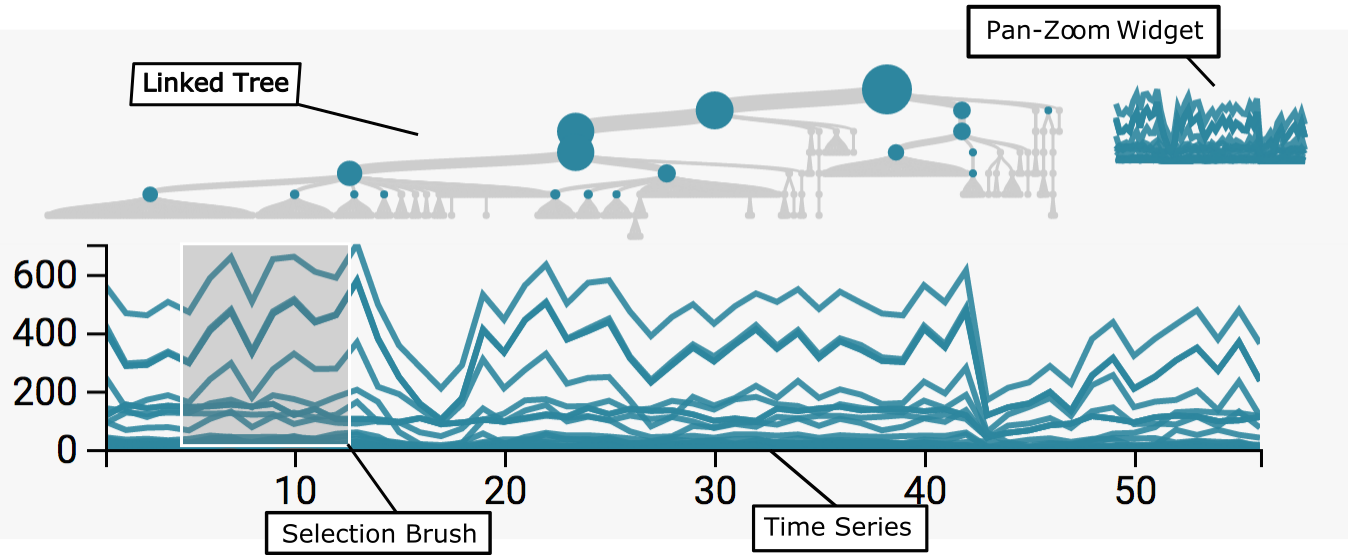
\includegraphics[width=375px]{figure/treelapse/annotated_antibiotic_overview}
  \caption{Here we display the primary timebox tree view of the antibiotics data
    set from \citep{dethlefsen2008pervasive}, annotated with the main components of the
    visualization. The tree at the top is a taxonomic tree of all the bacteria
    contained within the sample, and it is visually linked to the time series at
    the bottom: each node in the tree corresponds to a path among the time series.
    The selection brush is used to focus attention on the time series that go
    through it -- these are highlighted in blue -- and other brushes can be added
    using a button not displayed here. The pan-zoom widget at the top right is
    used to update the scales of the main time series display so that only
    particular time windows and $y$-axis ranges are visible. This view is the
    basis for all the timebox tree and treebox displays that appear
    below. \label{fig:antibioticoverview}}
\end{figure}

\begin{figure}

{\centering 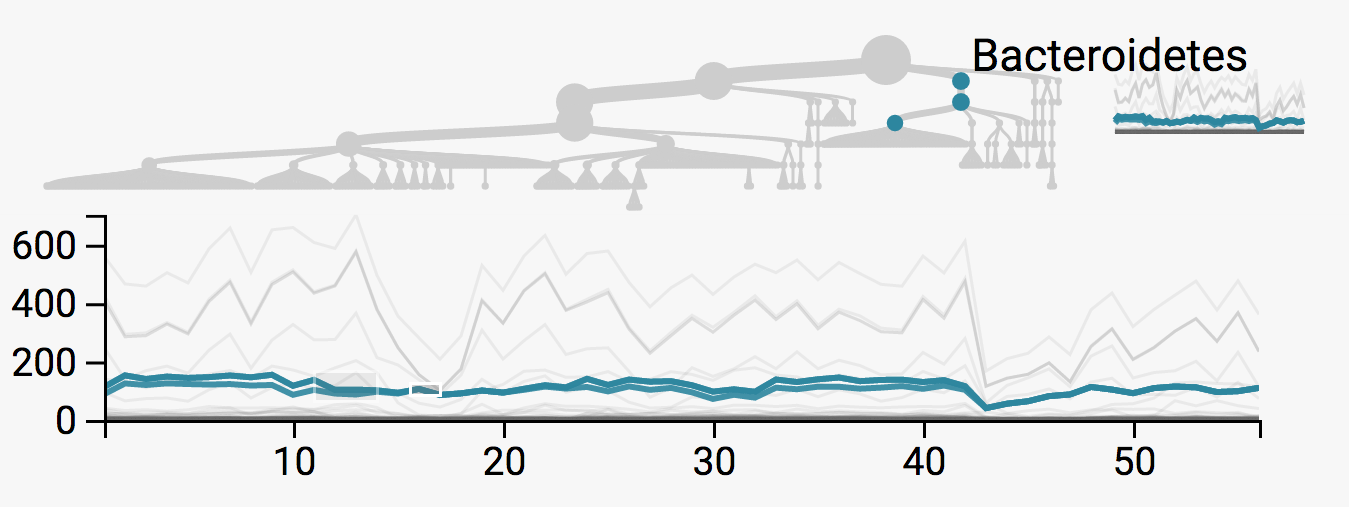
\includegraphics[width=375px]{figure/treelapse/antibiotic_bacteroidetes}

}

\caption{Introducing a second box into the timebox display identifies the
  Bacteroidetes as a taxon only mildly impacted by antibiotics. The layout is
  identical to Figure 1, except two small brushes are placed over the time
  series between 10 and 20 days, and now only those time series and
  corresponding nodes in the tree are highlighted in blue. Further, the user has
  hovered over the top blue node in the tree, revealing the taxonomic identity
  of these series. Hence, brushing the time series and linking with the tree can
  be used to discover and characterize notable variation within the
  data.\label{fig:antibioticbacteroidetes}}
\end{figure}

Next, using the scented widget, we focus on the window around the second
antibiotic treatment. We apply the treebox display to compare then behavior of
different families of Firmicutes, Lachnospiraceae and Ruminoccocus. We suspect
that these taxa are associated with the delayed recovery after the second time
course. To investigate this, we input these family names in the search box to
isolate their positions on the tree; then we apply brushes to highlight the
series that contribute to these higher-level families. The resulting view is
given by Figure \ref{fig:antibioticfirmicutes}

\begin{figure}
{\centering 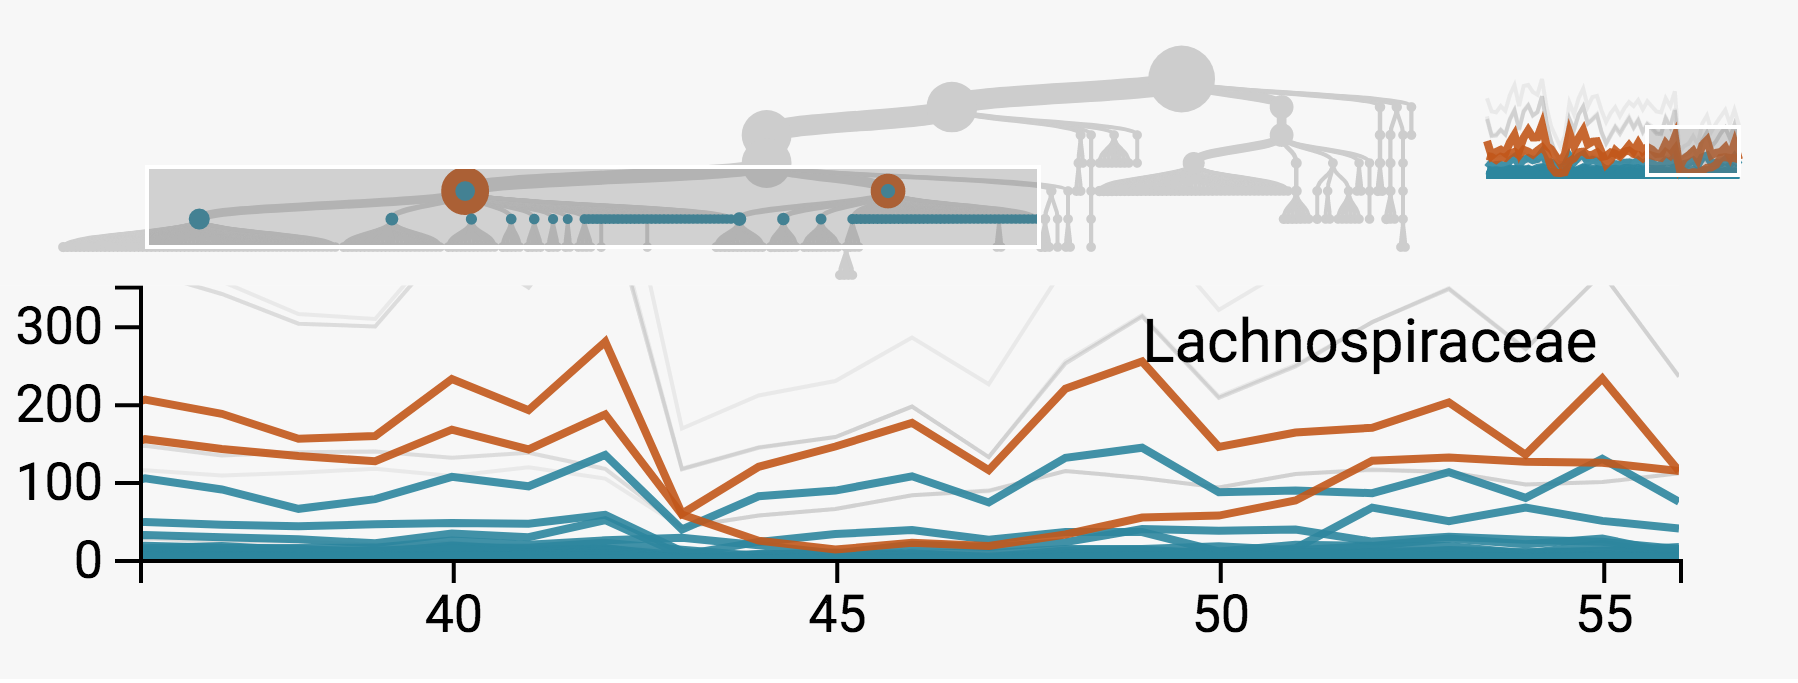
\includegraphics[width=375px]{figure/treelapse/antibiotic_firmicutes}

}

\caption{Zooming into the second antibiotic time course and highlighting the
  Lachnospiraceae and Ruminococcus, we see that the Ruminoccocus took more time
  to recover to pre-treatment levels. Here, the red lines and nodes are those
  that match the text search provided by the user in a search box just below the
  figure (not displayed here). Hovering the mouse over these lines provides
  their identities -- the top red line is Lachnospiraceae, and the bottom red
  line is Ruminoccocus. Note that the brush in the treebox display is located
  over the tree, rather than over the time series. In particular, the search box
  and interactive brushing can be combined to interrogate hypotheses of a priori
  interest. \label{fig:antibioticfirmicutes}}
\end{figure}

Alternatively, we can summarize each node by the average across its descendants
-- this brings attention to individual bacteria that may be underlying some of
the broader taxonomic patterns we have noted when studying the subtree sums. For
example, in Figure \ref{fig:ruminococcus}, we highlight all families below order
Ruminococcus, suggesting that the decrease due to antibiotics occurs uniformly
across almost all families. A point that was not evident in the earlier
sum-across-descendants view is that, after the second treatment of antibiotics,
a few of the Ruminoccocus families recover more rapidly than the rest, for
example the Unc095d3 (highlighted in red) are only briefly affected. In
contrast, most families seem to recover in unison after the first treatment.

\begin{figure}

{\centering 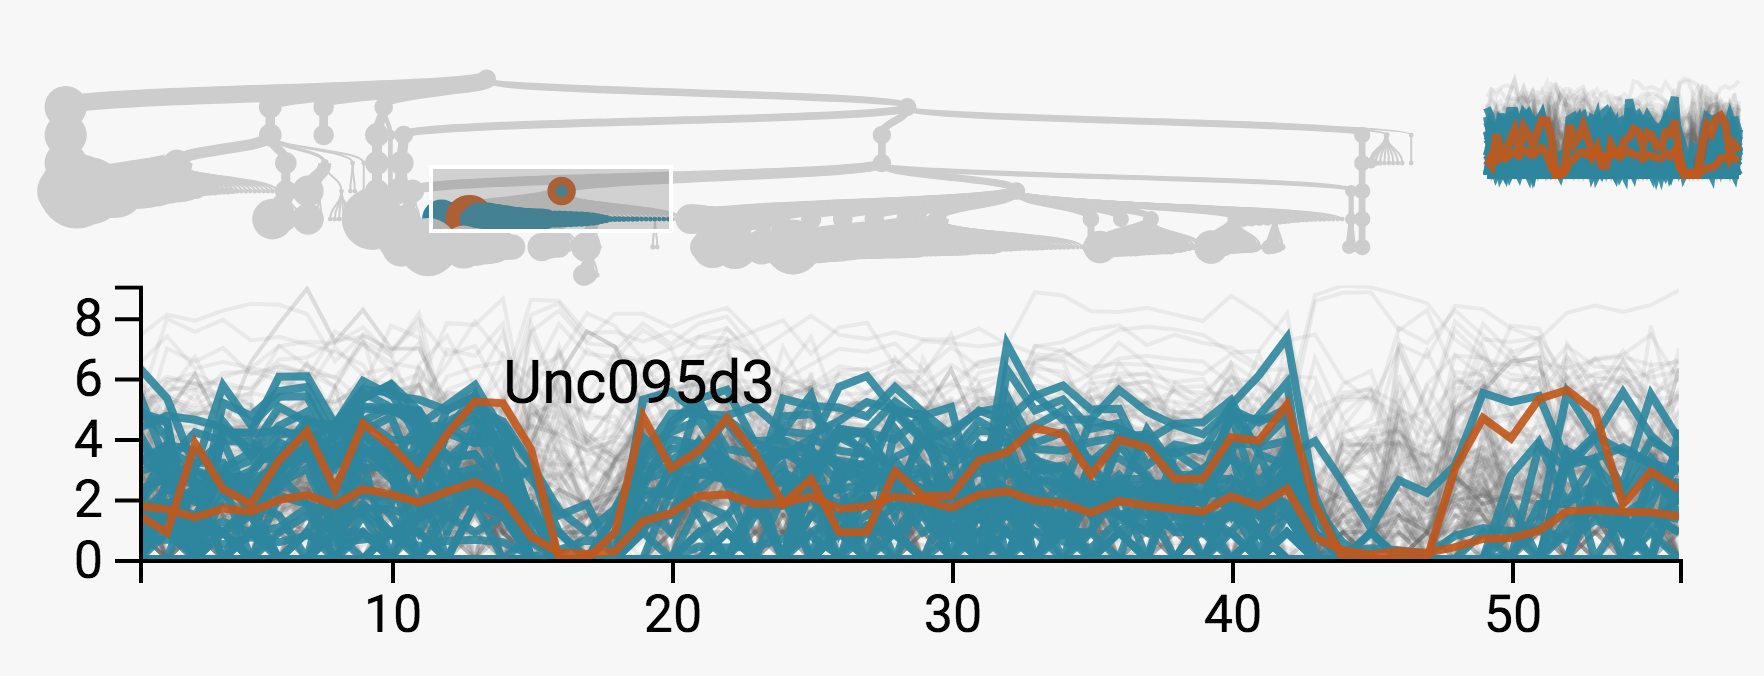
\includegraphics[width=375px]{figure/treelapse/ruminococcus}

}

\caption{By hovering over the Ruminoccocus branches, we see that there is a
  prolonged effect of the antibiotics time courses more or less uniformly across
  the lower taxonomic orders. The graphical elements are the same as before,
  except the user has searched for Ruminoccocus and species Unc095d3, which has
  the highest average abundance within this taxon. By displaying averages rather
  than sums, we see that the effect of antibiotics visible at higher taxonomic
  orders is not created by a single dominant species becoming less abundant, but
  rather the decline in populations across all descendant species. The same
  display applied to different data can yield different
  insights.}\label{fig:ruminococcus}
\end{figure}

Further, note that in this subtree averages view, the tree display has changed.
This is because, at each branching point, we place the node with larger average
value on the left. Figure \ref{fig:verrucomicrobiae} notes that the nodes at
the far left in the tree are associated with phylum Verrucomicrobiae,
corresponding to a large average abundance across time points. This phylum had
been previously obfuscated -- because there are not many leaves associated with
this phylum, the sum was small. Interestingly, the abundance of these bacteria
seems to \emph{increase} after the first antibiotics treatment. Be cautious,
however, that the average over only a few Verrucomicrobiae species will be a
more variable estimate than the averages over the more prevalent phyla.

\begin{figure}

{\centering 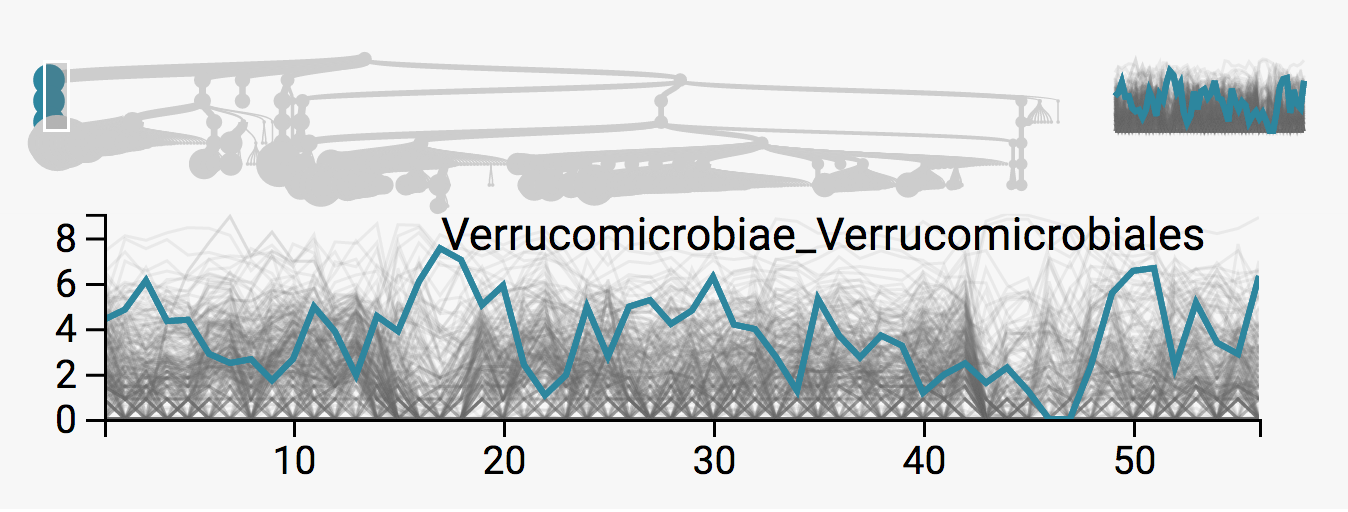
\includegraphics[width=375px]{figure/treelapse/verrucomicrobiae}

}

\caption{The subtree averages aggregation brings attention to the
  Verrucomicrobiae, which though only present as a few species, are each rather
  abundant. In particular, they seem to increase after the first antibiotic time
  course, which occurs between days 15 and 20. This view was generated by
  placing a brush over the branch on the far left, which has those nodes with
  the largest averages across all timepoints. The user's mouse is over the blue
  series, which brings up the associated taxonomic label. The determination of
  species whose abundances increase during antibiotics, which would require many
  hypothesis tests using a more standard approach, becomes quickly apparent
  via interactive visualization.}\label{fig:verrucomicrobiae}
\end{figure}

\subsubsection{Differential Bacterial Abundance and Preterm
Births}\label{differential-bacterial-abundance-and-preterm-births}

\citet{digiulio2015temporal}
tracked the abundance of bacteria in the vaginal microbiome during
pregnancy in an effort to study relationships between bacterial
community composition and preterm birth. Ideally, it would be possible
to develop clear bacterial signatures associated with preterm births.

Unlike the antibiotics study, we have measurements across more
individuals than we could reasonably inspect one at a time. While we
could average across all individuals, we will take our cue from
\citep{digiulio2015temporal}
place each sample into one of five Community State Types (CSTs),
identified via k-medoids. In that study, a linear model identified one
of these CSTs (CST 4) as significantly more diverse, further it appeared
associated with preterm births. Here, we corroborate this finding using
exploratory views.

Therefore, our focus here is on the differential abundance question,
rather than dynamics. We would like to provide visual representations of
differential abundance across CSTs and also between preterm and non-preterm
births. \citet{digiulio2015temporal} interpreted the CSTs using a heatmap, with
bacteria ordered according to a hierarchical clustering. By using the DOI sankey
instead, we can interpret the CSTs in their taxonomic context and at multiple
scales of taxonomic resolution. Further, while
\citet{digiulio2015temporal} focused on identifying associations between
preterm births and CSTs -- presumably because testing individual bacteria loses
power -- we can compare bacterial abundances between preterm and non-preterm
samples along subtrees, without requiring CSTs as an intermediary.

In Figure \ref{fig:pretermcsts}, we compare the 5 CSTs according to
their values along the subtree. Specifically, we took the average of all
samples within each CST to define values at the (species-level) leaf
nodes, and then aggregated the averages up to the root. It is
immediately clear that samples from CST 4 have much more taxonomic
diversity. Further, focusing on the Lactobacillaceae family, we note
that the differential abundance of these bacteria distinguishes the
remaining CSTs, see Figure \ref{fig:pretermcstslacto}.

Alternatively, in Figure \ref{fig:pretermpreterm}, we avoid working with CSTs,
displaying instead averages among samples associated with either preterm or term
births. The green and yellow edges are associated with preterm births -- we see
that they contribute more weight to phyla outside the Firmicutes. This is
consistent with the claim that CST 4, the most diverse of the CSTs, is
associated with preterm births.

\begin{figure}

{\centering 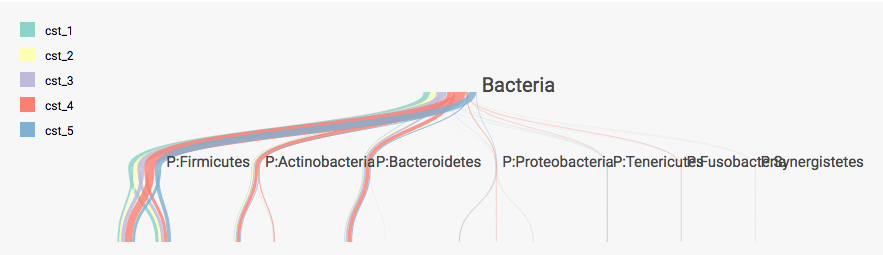
\includegraphics[width=375px]{figure/treelapse/preterm_csts}

}

\caption{The increased diversity among samples in community state type (CST) 4
  is represented by the relatively larger contribution of red edges to branches
  outside of the Firmicutes. This display shows the top of the DOI sankey
  visualization of the preterm birth data studied in
  \citep{digiulio2015temporal}. The root of the tree is the taxonomic kingdom
  Bacteria, its children are labeled according to their phylum names. Each color
  within a branch is associated with CST, and the width of the associated color
  corresponds to the average abundance of that taxonomic group among all samples
  belonging to the corresponding CST, as indicated by the legend at the left.
  Phyla are sorted from most to least abundant. This initial display of the DOI
  sankey provides a summary of overall abundances across taxonomic groups and
  CSTs, and suggests subtrees to navigate into, to extract more detailed
  abundance information.
}\label{fig:pretermcsts}
\end{figure}

\begin{figure}

{\centering 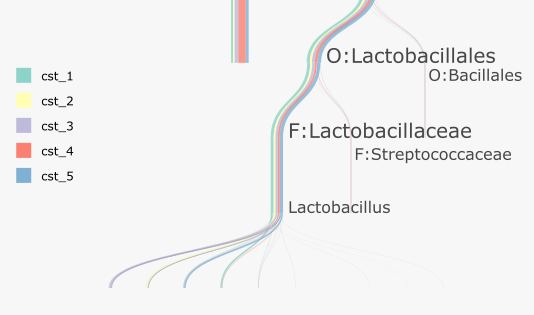
\includegraphics[width=375px]{figure/treelapse/preterm_csts_lacto}

}

\caption{Zooming into the Lactobacillaceae family, we notice that the difference
  between the remaining four CSTs is related to which types of Lactobacillus are
  most prominent. The DOI sankey refocuses the tree around the last group that
  was clicked on, in this case showing more detail about order Lactobacillales
  and its descendants. The overview display can be recovered by navigating back
  up to higher-level taxa. Hence, it is possible to navigate between broad
  overview and detailed displays in a way that facilitates interpretation of
  results from statistical analysis.}\label{fig:pretermcstslacto}
\end{figure}

\begin{figure}
\centering
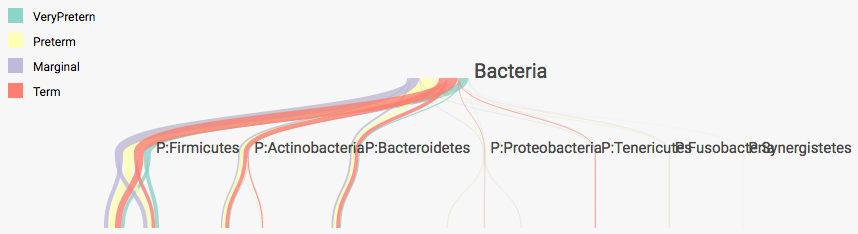
\includegraphics[width=300px]{figure/treelapse/preterm_preterm}
\caption{Samples with high levels of phyla other than Firmicutes appear to be
  related to preterm births. Here, we again display the preterm birth data with
  a DOI sankey, but instead of grouping samples according to statistically
  generated CSTs, we directly assign samples to preterm vs. not preterm
  according to whether the mother eventually had a preterm birth. These new
  states are visible in the updated legend. Through interactivity, it becomes
  possible to develop meaningful visual summaries even before calculating formal
  statistical ones.}
\label{fig:pretermpreterm}
\end{figure}

\subsubsection{Dynamics in Housing Prices}\label{zillow-study}

We next consider an application unrelated to the microbiome, but with relatively
clear hierarchical structure. Our data are downloaded from Zillow and give the
Zillow Home Value Indexes at the neighborhood level, across the country,
computed monthly between 1996 and 2016. A link to the data source is provided in
the supplementary materials. In our display, we have taken the natural log of
these indexes. As our hierarchical structure, we use each neighborhood's
assignment to state, regional, county, and city levels. We represent each of
these coarser spatial categories using the average of all neighborhoods
contained in them. We have filtered down to the 890 neighborhoods in California;
rendering more neighborhoods while keeping all 246 timepoints causes a severe
lag in the interface.

Our basic analysis revolves around geographic and temporal variation in home
prices. We are especially interested in the effect of the 2008 recession and any
variation in the lead-up to or recovery from this event. These questions can be
naturally framed using timebox trees and treeboxes.

For example, we can study the trajectories of home prices among neighborhoods,
conditional on their being middle-income before the recession. We generate the
sequence of views in Figures \ref{fig:zillowmiddlepre},
\ref{fig:zillowmiddleup}, and \ref{fig:zillowmiddledown} to this end. The first
of these figures isolates neighborhoods with middle incomes before the
recession, using a single timebox. Since there appears to be a divergence in
trajectories after the recession, we introduce a second post-recession timebox,
dragging it over series with higher and lower incomes during this second time
period. This is the content of Figures \ref{fig:zillowmiddleup} and
\ref{fig:zillowmiddledown}. Though not directly visible from the static figures,
hovering the mouse over the highlighted tree nodes provides the geographic
identities, and we find that most of the middle-income series that increased
after the recession are associated with middle-income neighborhoods within the
coastal Southern California counties. For example, the mouse is currently over a
subtree with many highlighted nodes, which is shown to be the Los Angeles-Long
Beach-Anaheim metropolitan area. In contrast, hovering over nodes associated
with those middle income neighborhoods that saw decreases indicates that they
were mostly located in Central California and Oakland. In Figure
\ref{fig:zillowmiddledown}, the mouse is positioned over the Sacramento (which
is located in Central California) subtree, and seems enriched for this subset of
strongly recession-affected series.

The previous analysis highlights the fact that, within even narrow geographic
regions, there can be substantial variation in prices. We can study this
directly using treeboxes. In Figure \ref{fig:zillowsf} we have highlighted all
series in San Francisco County. We see that, in 2016, prices range from around
$e^{13} \approx \$440,000$ to $e^{14.5} \approx 2 \text{ million}$. So,
while all these neighborhoods tend to be among the more expensive ones in
California, prices can vary in a non-smooth way across geographic space.

We conclude this example with a caveat that the Zillow data are not
representative of all neighborhoods in California, only those with enough
listings on the site, so should be supplemented by other data sources for any
substantial decision-making.

\begin{figure}

{\centering 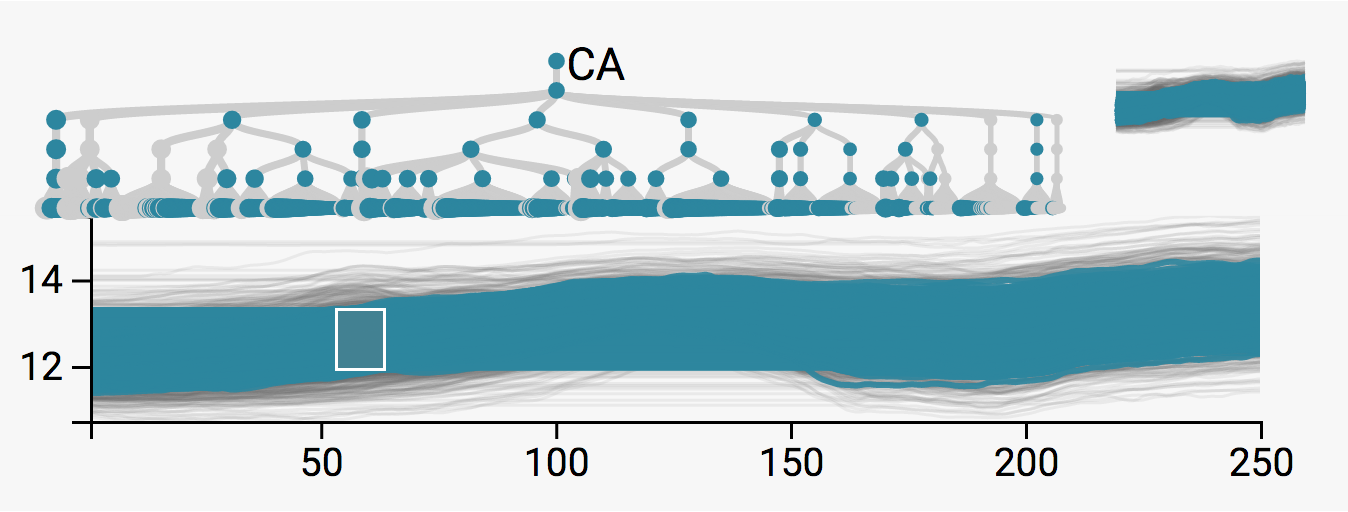
\includegraphics[width=375px]{figure/treelapse/zillow_middle_pre}

}

\caption{The time series here represent California neighborhood home prices
  between 1996 and 2016, and the tree corresponds to a geographic hierarchy,
  with regions at the top and neighborhoods at the bottom. We have brushed the
  neighborhoods with mid-range home prices before the recession. The associated
  tree nodes are highlighted at the top. Note that the collection of series
  seems to widen after 2008 -- we are interested in whether there are reliable
  predictors of these alternate trajectories, given their similar starting
  points. This serves as a baseline with which to compare Figure
  \ref{fig:zillowmiddleup} -- these views are easy to transition between
  interactively.}\label{fig:zillowmiddlepre}
\end{figure}

\begin{figure}

{\centering 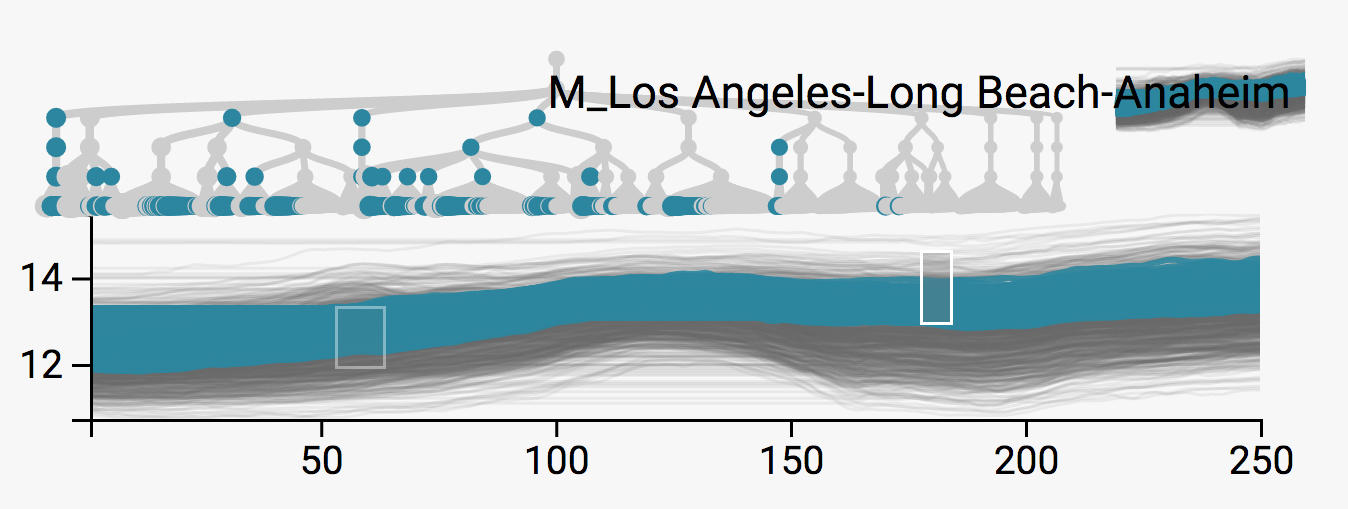
\includegraphics[width=375px]{figure/treelapse/zillow_middle_up}

}

\caption{Among those neighborhoods with mid-range prices before the recession,
  displayed in Figure \ref{fig:zillowmiddlepre}, we have selected those that
  recovered more rapidly by introducing a brush at the top right of the time
  series panel. By hovering a brush over a collection of tree nodes that all
  seem to be highlighted, we infer that the associated neighborhoods are located
  mainly in Los Angeles and San Diego counties. This follow-up view is
  interesting to contrast with Figure \ref{fig:zillowmiddledown}.
}\label{fig:zillowmiddleup}
\end{figure}

\begin{figure}

{\centering 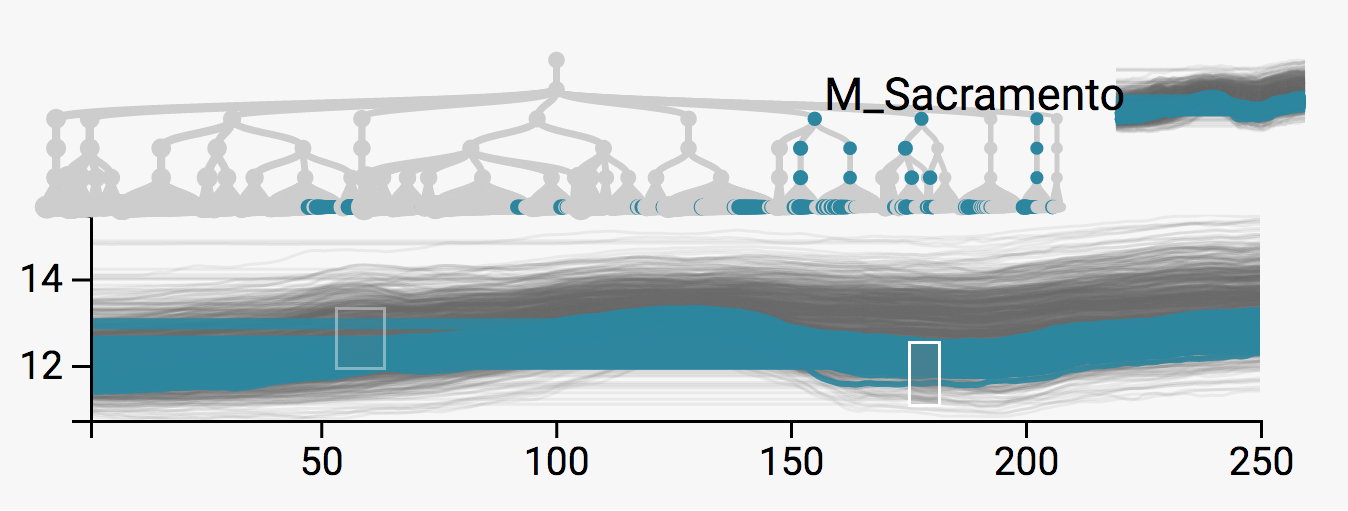
\includegraphics[width=375px]{figure/treelapse/zillow_middle_down}

}

\caption{In contrast to Figure \ref{fig:zillowmiddleup}, we can follow-up the
  selection in Figure \ref{fig:zillowmiddlepre} by isolating those neighborhoods
  where prices remained depressed after the recession. This is accomplished by
  moving the brush on the right down towards lower prices. Hovering over the
  associated highlighted nodes in the tree to reveal the associated locations,
  we see that most of these series correspond to neighborhoods in Central
  California and the East San Francisco Bay Area. The ability to sketch the
  overall shapes of series using brushes and interpret the associated selections
  using a tree simplifies what might otherwise be complex
  comparisons.}\label{fig:zillowmiddledown}
\end{figure}

\begin{figure}

{\centering 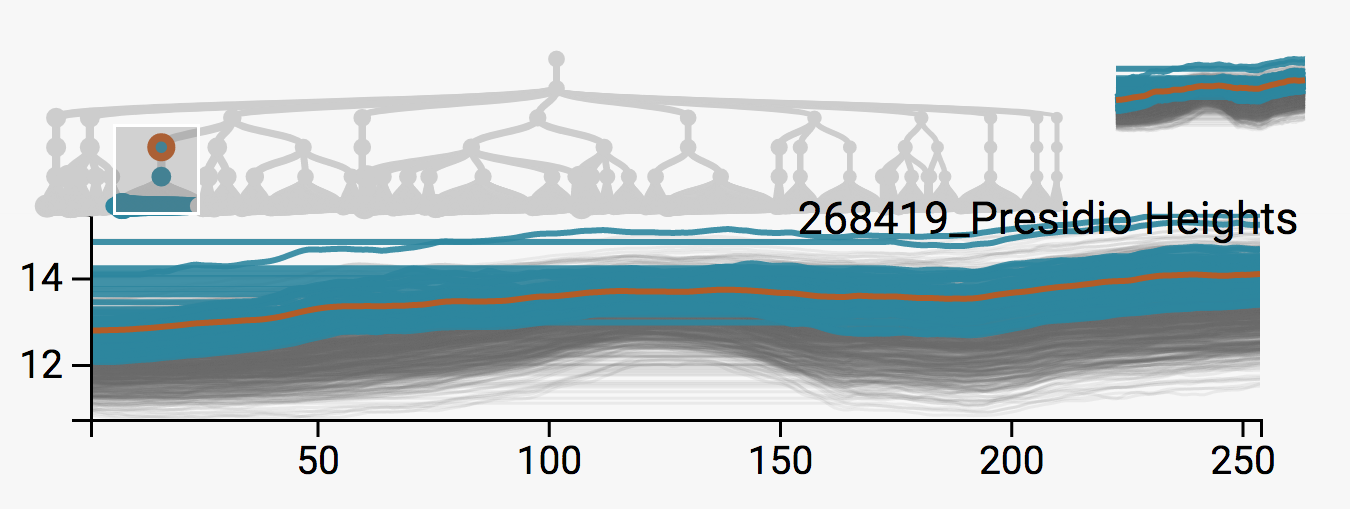
\includegraphics[width=375px]{figure/treelapse/zillow_sf}

}

\caption{In contrast to Figures \ref{fig:zillowmiddlepre} to
  \ref{fig:zillowmiddledown}, we can study the variation in series associated
  with a subset of the tree by using treeboxes. To study the range in home
  prices within San Francisco County, we can brush over the associated nodes in
  the tree. The red circle indicates that the user has searched for ``San
  Francisco,'' which guides the user to the appropriate subtree. The mouse is
  hovering over one of the more expensive neighborhoods. Hence, though the
  timebox tree and treebox views are similar, they are directed towards
  different types of visual comparisons.}\label{fig:zillowsf}
\end{figure}

\subsubsection{Sources of Variation in Bikesharing
Demand}\label{bikesharing-study}

Our next example is a study in bikesharing demand, included as an example of
analyzing collections of time series when there is no obvious hierarchical
structure a priori. The data are available at the UCI Repository and were
originally collected by a Washington D.C.-based bikesharing system for use in a
Kaggle prediction competition. A link is provided in the supplementary
materials. The data are hourly measurements of bike demand, aggregated across
all bikesharing stations, over two years, along with supplemental weather data.
In the competition, participants were asked to predict the hourly demand on a
held-out test set. Here, we adopt a descriptive view instead, attempting to
characterize factors associated with variation in bikesharing demand.

Like the Zillow home prices application, we study this problem as one of
describing a large collection of related time series. Here, we consider
the demand during a single day to be one time series; this is a natural
choice considering the daily periodicity of bike demand. To arrange
these daily series along an interpretable tree structure, we apply a
regression tree relating the supplemental data to the bikesharing demand
\citep{breiman1984classification}. In more
detail, we built this tree by noting the ``two table'' structure of this
problem: one describes bike demand, the other holds the supplemental
data. In both, the rows index days, while the columns index either hours
or supplemental features. Our tree is the trained regression tree after
predicting demand at 8AM based on the supplemental data. We choose this
response because (1) we need a univariate response in order to apply
regression trees and (2) the more straightforwards reduction to
daily-average-demand fails to distinguish between weekdays and weekends,
whose series appear qualitatively very different from each other.

Given this response, the first split in the regression tree is
(unsurprisingly) the difference between weekends and weekdays. This is
emphasized in Figures \ref{fig:working} and \ref{fig:weekend}, respectively;
using timeboxes to isolate the two types of series highlight the left and right
sides of the tree, respectively. For a more subtle effect, we select the
internal nodes associated with the first split below the weekday vs. weekend
split; these are given in Figures \ref{fig:weekday2011} and
\ref{fig:weekday2012}. This suggests that weekday demand increased during the
second year.

\begin{figure}

{\centering 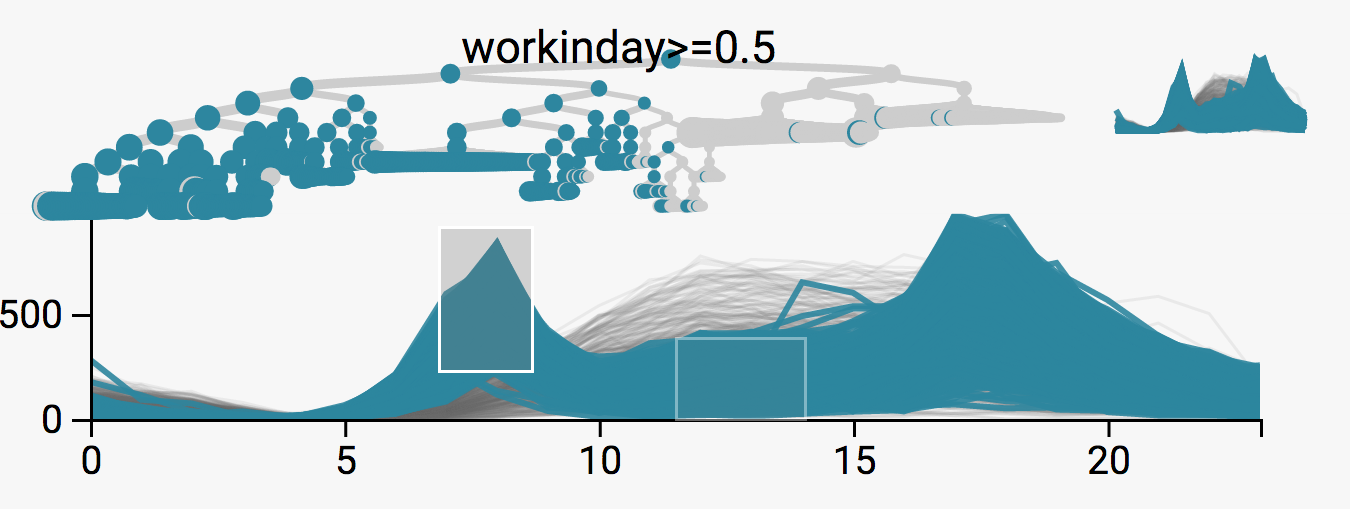
\includegraphics[width=375px]{figure/treelapse/working}

}

\caption{The two peaks at rush hour distinguish weekday series from the rest.
  through the timebox tree view. The display is the same type of timebox tree
  view introduced in Figure \ref{fig:antibioticoverview}, but applied to the
  bikesharing data, where the time axis represents the time of day and the
  $y$-axis gives bikesharing demand. Each series is the bikesharing demand for a
  single day, over the course of two years. The tree now corresponds to the
  regression tree generated by predicting demand at 8am using supplementary
  data. Two brushes are introduced to highlight the double peaks corresponding
  to rush hours on weekdays. We see that although hierarchical structure was not
  present immediately in the bikesharing data, it is useful to introduce and
  interpret such structure by combining regression and visualization
  methodology.
}\label{fig:working}
\end{figure}

\begin{figure}
  \centering
  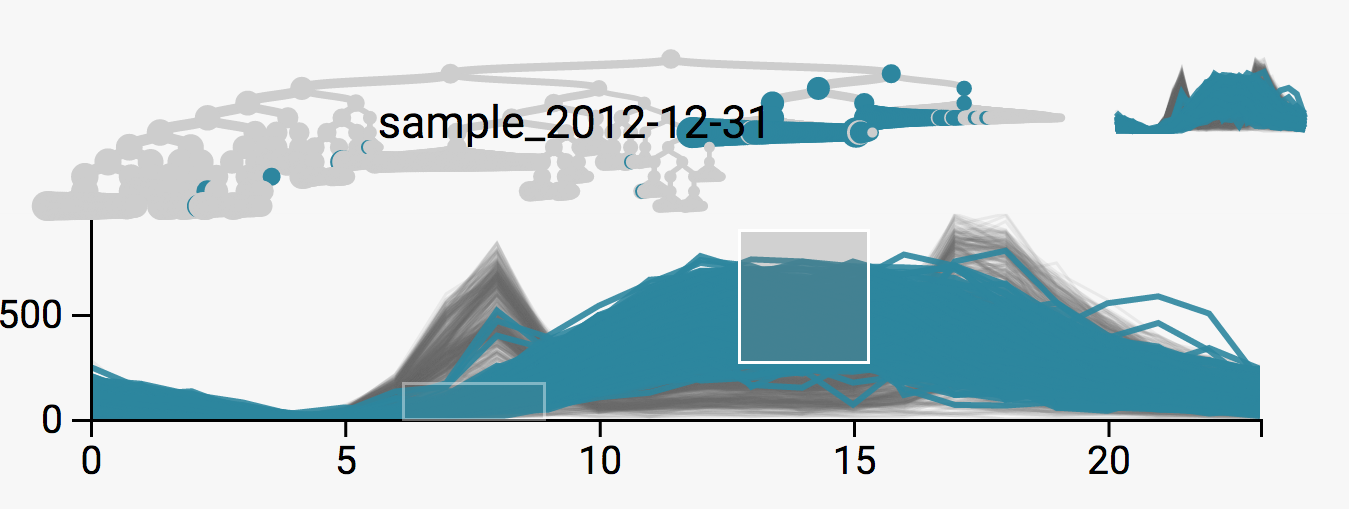
\includegraphics[width=375px]{figure/treelapse/weekend}
    \caption{By adjusting the two brushes in Figure \ref{fig:working}, we see that
      unlike weekday demand, weekend demand is unimodal. The few weekday series with
      unimodal series seem to be associated with holidays. This is the case for New
      Years' Eve, which is currently hovered over in the tree. The ease of
      transitioning from Figure \ref{fig:working} to this display indicates the
      importances of brushing in interaction.}\label{fig:weekend}
\end{figure}

\begin{figure}
  \centering
  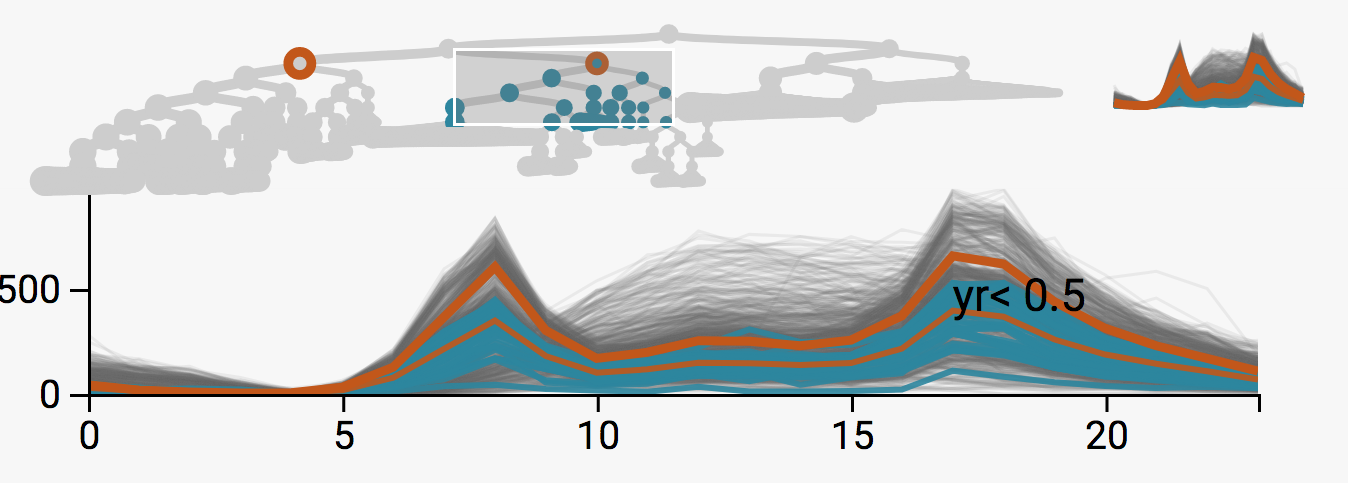
\includegraphics[width=375px]{figure/treelapse/weekday_2011}
    \caption{Weekday demand appears larger in 2012 than 2011 -- compare with Figure 
      \ref{fig:weekday2012}. Here, a brushes are introduced over the tree to see the
      series associated with a particular split point. The red nodes are the results
      of searches over the two nodes that are children of this split point. The fact
      that the \texttt{yr>=0.5} selected line is larger than the \texttt{yr<0.5}
      line means that demand was larger in 2012. In combination with searching and
      treeboxes, it is possible to interpret more subtle split points in the decision
      tree.} \label{fig:weekday2011}
\end{figure}

\begin{figure}
  \centering
  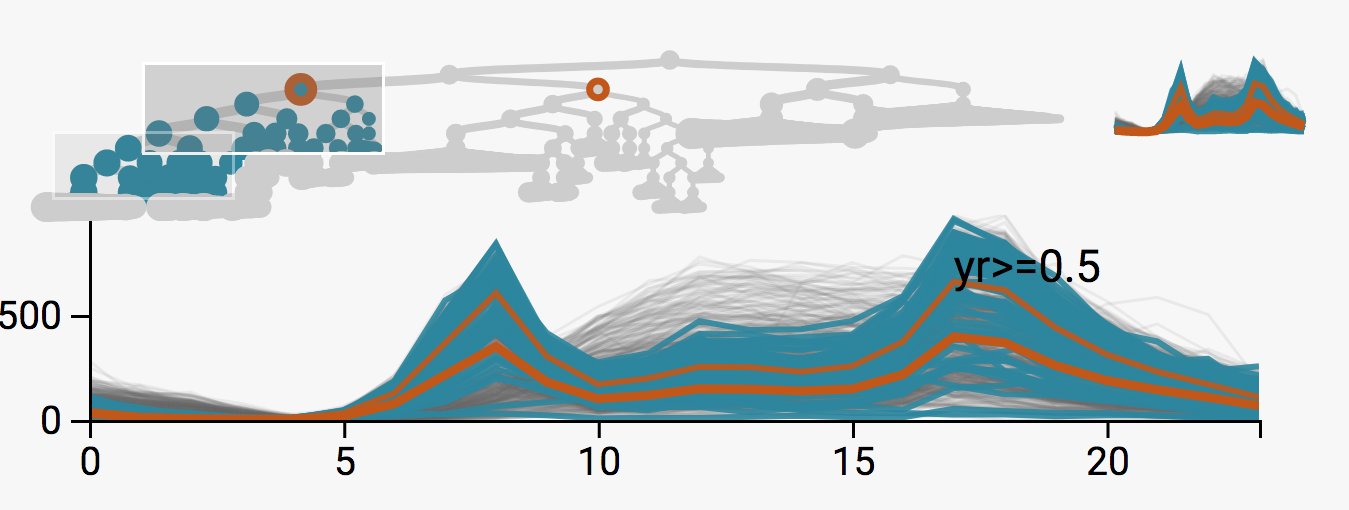
\includegraphics[width=375px]{figure/treelapse/weekday_2012}
  \caption{Weekday demand increased in 2012 -- compare with 
    Figure \ref{fig:weekday2011}. The search terms are the same as in that figure,
    but the subtree associated with the 2012 split point is highlighted, using the
    union of two boxes. Note that unlike timebox trees, which highlighted series
    lying through the intersection of brushes, treeboxes highlight series within the
    union of brushes.}\label{fig:weekday2012}
\end{figure}

In contrast to these general questions about daily demand, we could ask
a more granular question about specific time windows. For example, what
characterizes days on which there is larger than average demand after
midnight? We can select these series after first zooming into this time window.
Figure \ref{fig:warmweekend} reveals that the highlighted series are associated
with the warm-weekend split, which seems quite reasonable in retrospect.

\begin{figure}

{\centering 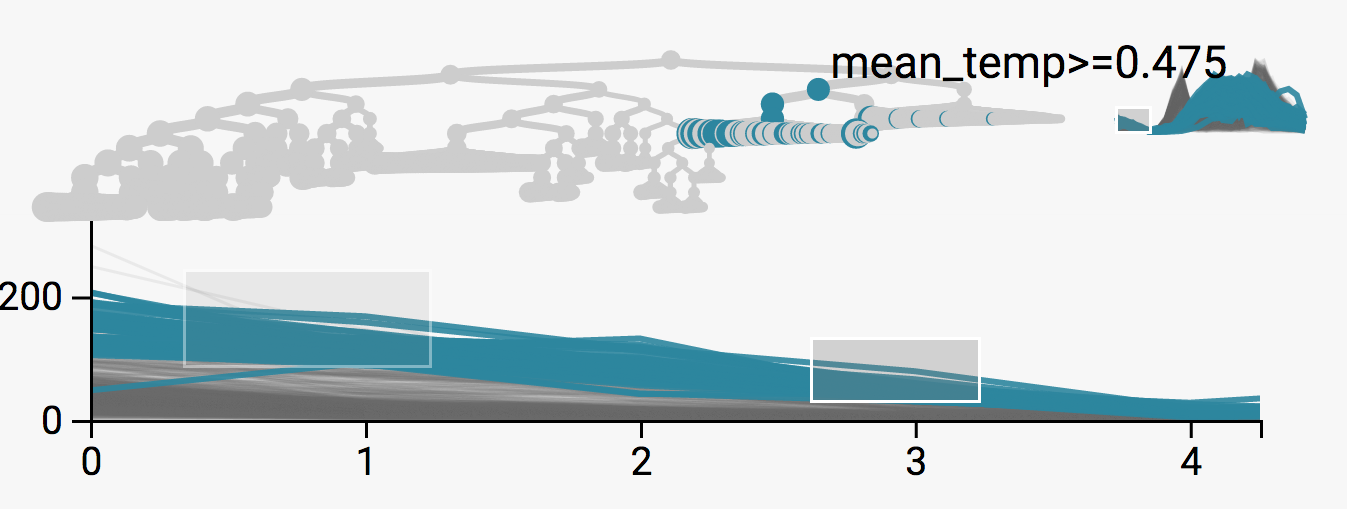
\includegraphics[width=375px]{figure/treelapse/warm_weekend}

}

\caption{The samples with highest night demand tend to fall on warm
  weekends. Here, the pan-zoom widget has been used to adjust both time and
  demand axes to narrow on a specific window of interest. Brushes are drawn over
  the larger among these series, and the corresponding tree nodes are located
  close to one another, in the part of the tree corresponding to the warm / cold
  average temperature split. More generally, panning and zooming allows
  navigation between focus and context.}\label{fig:warmweekend}
\end{figure}

Finally, we can study the behavior of the regression tree itself using
the DOI sankey. Here, we group samples according to their quintile of
8AM demand and then count the abundance of the groups flowing down
different branches. We find that the quintiles are each rather strongly
separated after descending even a few steps down the regression tree --
for example, Figures \ref{fig:weekday2011} and \ref{fig:weekday2012}
focus on 2011 vs. 2012 split among weekday samples, showing that this
split distinguishes between samples falling in the second and third
quintiles of 8AM demand.

\begin{figure}

{\centering 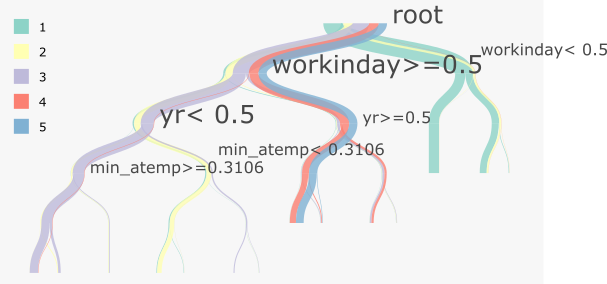
\includegraphics[width=375px]{figure/treelapse/bike_sankey}

}

\caption{So far, we have focused on the timebox tree and treebox representations
  of the bikesharing data -- a complementary view is provided by the DOI sankey.
  Here, the tree is the result of the regression tree procedure, while the
  colors represent particular quantiles of 8am demand. This allows the
  determination of which split descendants are associated with low or high
  demand.}\label{fig:bikesankey}
\end{figure}

This interactive representation of regression trees is potentially more
useful on larger trees that cannot be easily parsed in a single view; in
this sense the bikesharing tree is relatively simple. In our ideal data
analysis workflow, we imagine the analyst applying interactive
visualization and modeling techniques in an iterative, nonlinear
fashion, in the spirit of \citep{de2003visual}.

\subsubsection{Hierarchically Clustering the Global Patterns Data}\label{global_patterns}

Each of the timebox tree and treebox examples presented so far have
focused on data with a clear time component. We note however that these
techniques could alternatively be applied to high-dimensional data, via
the use of parallel coordinates \citep{inselberg1991parallel}. The usual
parallel coordinates challenges remain, namely selecting scales for and an
ordering across the different coordinates, but the linking and
focus-plus-context ideas can still be employed in this setting. Here we
provide an implementation of this idea on a dataset comparing microbiomes across
various ecological environments \citep{caporaso2011global}, which is publicly
accessible through the phyloseq R package \citep{mcmurdie2013phyloseq}.

The original Global Patterns data consists of 26 samples across 9
environments (for example, freshwater and soil). In each site, there are
counts across 19216 taxa -- to simplify visualization, we filter to the
500 most abundant taxa.

We hierarchically cluster these 26 samples based on the 500 most
abundant taxa, using complete linkage on the UniFrac distance. Figure
\ref{fig:gptimebox} displays the resulting hierarchy together with a
parallel coordinates view of the \(\text{asinh}\) transformed taxa.

\begin{figure}
  {
    \centering
    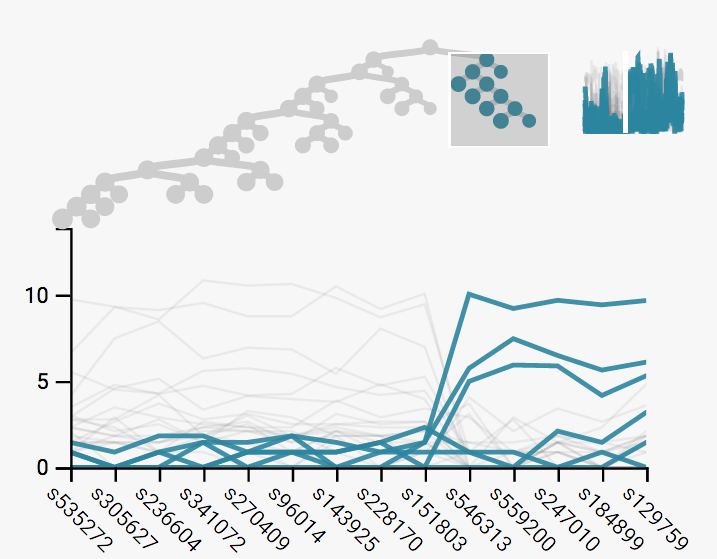
\includegraphics[width=225px]{figure/treelapse/gp_cluster1}
    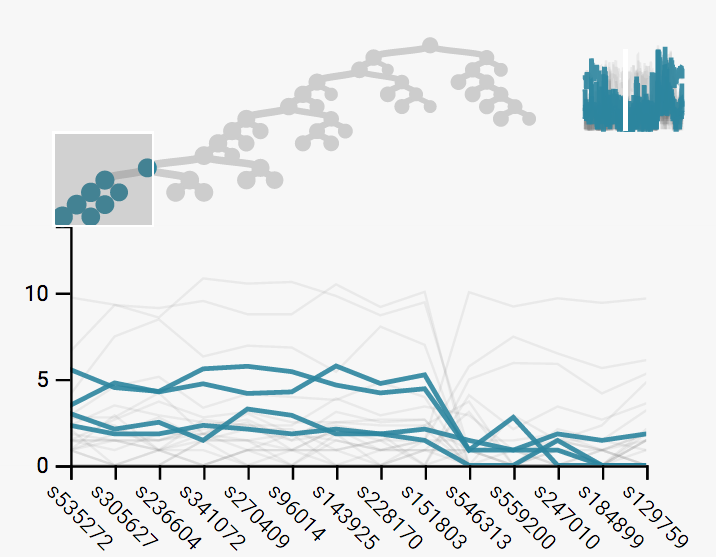
\includegraphics[width=225px]{figure/treelapse/gp_cluster2}
}

\caption{An application to the Global Patterns demonstrates how linking in
  treelapse can be applied to combine hierarchical clustering and parallel
  coordinates views. Each panel represents a different subtree cluster within
  this data set, as indicated by the different locations for the tree brushes.
  The paths in the lower halves of each display represent the average value
  across different bacteria rather than timepoints, as in all previous figures.
  Though the samples originally do not include any hierarchical structure,
  hierarchical clustering provides such a structure which can then be
  interpreted using treeboxes.}\label{fig:gptimebox}
\end{figure}

In Figure \ref{fig:gptimebox}, we compare two subclusters from the
hierarchical clustering tree, after zooming to a few of the bacteria
that distinguish between the clusters. In contrast to the figures displayed to
this point, we only print time series associated with observed samples -- the
leaves of the hierarchical clustering tree. This reduces visual artifacts that
can be created by plotting many similar internal nodes, and which can overwhelm
patterns occuring in the leaves, which are those of central interest. Upon
revisiting the original data, it becomes clear that the samples highlighted on
the left come from freshwater samples, while those on the right come from soil
and skin, and looking up taxonomic groups associated with the distinguishing
bacteria confirms this. For example, many of the species with high
abundances in the left figure come from order Oceanospirillales.

\subsubsection{Inspecting Confirmatory Analysis}\label{structssi}

In addition to facilitating exploratory study, treelapse has potential
value as a device for inspecting confirmatory analysis. We provide an
illustration extending an example from \citep{callahan2016bioconductor}, which
formally tested bacterial species for association with age in a sample of mice.
The testing approach advocated there is particularly well-suited to
visualization with treelapse, since it sought to detect associations at multiple
levels of phylogenetic resolution, using statistical tools developed in
\citep{yekutieli2008hierarchical, sankaran2014structssi}.

The data of interest in \citep{callahan2016bioconductor} are bacterial counts
collected across old and young mice. After variance-stabilizing these counts
using DESeq2 \citep{love2014moderated}, a $t$-test was applied to each node in a
phylogenetic tree, comparing abundances between old and young mice. To account
for multiple testing, we employ the structSSI algorithm
\citep{yekutieli2008hierarchical, sankaran2014structssi} along with methods
available in the \texttt{multtest} package \citep{pollard2005multiple}.

To interpret the results, we apply timebox trees. Our goals are to (1) identify
subtrees with consistently elevated differential abundance across age groups and
(2) compare alternative multiple testing adjustment procedures. Our approach is
to display the negative-log raw and adjusted $p$-values for each node, with
alternative methods compared via parallel coordinates. One view of the resulting
display is captured in Figure \ref{fig:structssi}. First, we see that
significant nodes tend to be significant across all methods -- the ordering
between different series appears stable. Interestingly, the Sidak one-step and
structSSI procedures seem to have lower power than the others, including
conservative FWER-controlling methods, like the Bonferroni procedure. Further,
in this application, FDR-controlling techniques do not seem to offer notably
different adjusted $p$-values, relative to those controlling FWER. This suggests
that, for this problem, bacteria are either strongly associated with age, or not
associated at all, so that there is little gain from using more sensitive
procedures.

\begin{figure}

{\centering 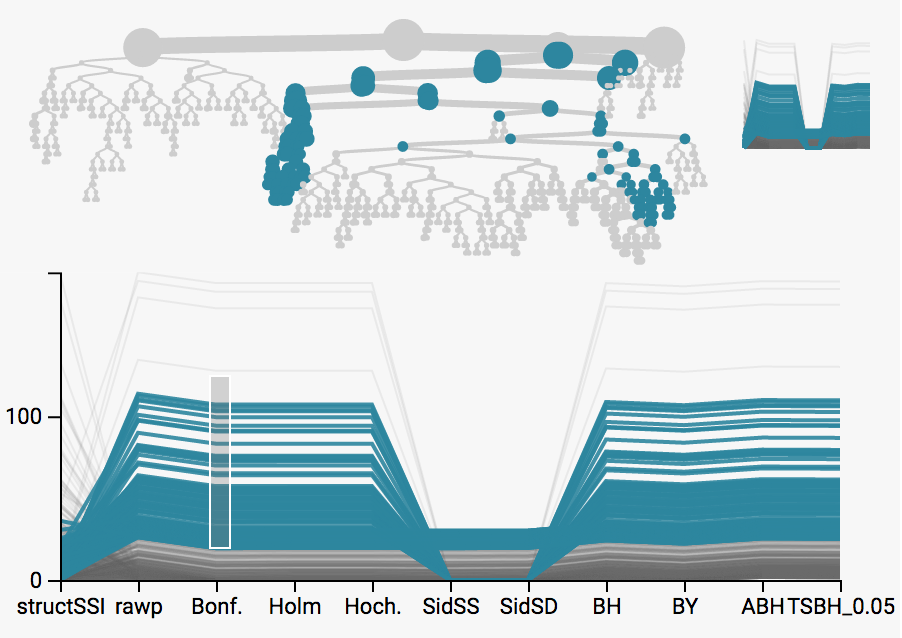
\includegraphics[width=325px]{figure/treelapse/structssi}

}

\caption{Viewing a tree of $p$-values across different methods highlights two
  subtrees with strong associations with mouse age, across several testing
  procedures. The tree represents the taxonomy of bacteria, and the series
  provides the negative log $p$-values associated with nodes as computed by
  different tests, listed along the $x$-axis as in parallel coordinates. By
  selecting series with larger values for a test, we see the associated subtrees
  of significant $p$-values. Hence, hierarchical views can be useful even in the
  confirmatory testing settings which typically study results from individual
  tests in isolation from each other.\label{fig:structssi}}
\end{figure}

Further, selecting series with strong association between abundance and age, two
major subtrees are brought to the forefront. Separately querying the
taxonomic identities of these bacteria reveals that they are two subgroups of
Clostridia, which is consistent with the analysis of
\citep{callahan2016bioconductor}. More than this specific analysis outcome, this
view demonstrates that interactive visual inspection of results from
confirmatory analysis provides deeper insight than the standard practice of
printing tables of (adjusted or unadjusted) $p$-values: the relationship between
significant nodes is only clear upon visualization on the tree.

\section{mvarVis}

mvarVis is an R package for visualization of diverse multivariate analysis
methods. We implement two new tools to facilitate analyses that are cumbersome
with existing software. The first uses htmlwidgets and D3 to create interactive
ordination plots, while the second makes it easy to bootstrap multivariate
methods and align the resulting scores. These interactive visualizations offer an
alternative to printing multiple plots with different supplementary information
overlaid, and bootstrapping enables qualitative assessment of the uncertainty
underlying the application of exploratory multivariate methods on particular
data sets.

Our approach is to leverage existing packages -- FactoMineR, ade4, and vegan
\citep{le2008factominer, dray2007ade4, oksanen2007vegan} -- to perform the
actual dimension reduction, and build a new layer for visualizing and
bootstrapping their results. This allows our tools to wrap a variety of existing
methods, including one table, multitable, and distance-based approaches --
principal components, multiple factor analysis, and multidimensional scaling,
for example. Since our package uses htmlwidgets, it is possible to embed our
interactive plots in Rmarkdown pages and Shiny apps
\citep{vaidyanathan2014htmlwidgets}. All code and many examples are available on
our github page: \url{https://github.com/krisrs1128/mvarVis}.

\subsection{Motivation}

The analysis of complex data sets often requires a dimensionality reduction
step. Common methods for dimensionality reduction or feature extraction are
principal component analysis (PCA), canonical correlation analysis (CCA),
nonlinear multidimensional scaling (NMDS). While there are a number of R
packages for multivariate analysis, they often have a steep learning curve and
rarely share common code conventions. Further, data input and output formats
oftne vary largely from one package to the other. Finally, most packages
generate static results, an unnecessary limitation, in light of increasingly
accessible interactive visualization tools in the data analysis community.

mvarVis unifies different ways of performing multivariate analysis and
facilitates the process of generating visualizations. It is build on top of the
existing statistical packages, but adds a a layer of interactivity to the
resulting visualizations. With mvarVis, the user can easily add and display
supplemental information. Additionally, the package incorporates a bootstrapping
tool for resampling the input data. Bootstrapping is used to assess the
stability of the results of the analysis. The uncertainty of the dimensionality
reduction techniques can be estimated for example by inspecting the ordination
plots with bootstrapped samples.

\subsection{Principles}

The design of mvarVis reflects a few guiding principles,
\begin{itemize}
\item Identify ways to ease interpretation of existing implementations of
  multivariate analysis methods, but avoid developing new implementations or
  methods.
\item Leverage interactivity to facilitate users' navigation through alternative
  dimension reduction views.
\item Put checks in place to ensure correct conclusions are drawn from analysis
  results.
\end{itemize}

We detail these points below. The first point motivates links between mvarVis
and implementations in FactoMineR, ade4, and vegan. Our approach modularizes the
task into (1) converting the output from these packages to a consistent S4 class
and (2) creating visualization and interpretation tools that operate on this
class. By separating the implementation in this way, it is easy to extend
mvarVis on both fronts without risking incompatibilities elsewhere.

The second point was motivated by the observation that, in practice, to
understand multivariate analysis results, it is often necessary to iterate
across many types of supplemental information in order to characterize latent
dimensions. For example, when viewing the output of a PCA, it is common to color
points by many different variables which were not used in producing the
dimension reduction. By making this process interactive, we hope to help viewers
find meaningful patterns with less effort.

Finally, we take responsibility for correct interpretation of the displays
produced by mvarVis. One first check is to fix coordinate axis scalings to
reflect the proportion of variance explained by each axis
\citep{fukuyama2017multidomain}. Second, we provide methods for bootstrapping
results to assess ordination uncertainty -- points with wide contours should be
interpreted with caution \citep{efron1992bootstrap}.

\subsection{Implementation}

mvarVis uses an S4 class, which we call an mvarLayer, as a fundamental building
block unifying output from other ordination packages. Each layer is composed of
coordinates of projected points along with supplemental information describing
it.

Different tables, or types of coordinates, become different layers. The
interactive displays are created using D3, with communication between D3 and R
enabled by the htmlwidgets package \citep{vaidyanathan2014htmlwidgets}.

\subsection{Bootstrap}

In many application it is of interest to assess the degree of stability in the
lower-dimensional representations of the data. The uncertainty in the
coordinates of the data points in the reduced space can be estimated in some
cases where the input data are counts or proportions, e.g. community composition
or gene expression data. For examlpe, this can be done by,
\begin{itemize}
\item Bootstrapping the input data matrix.
\item Applying the multivariate analysis to each of the bootstrapped samples.
\item Plotting all bootstrapped points together in the reduced space.
\end{itemize}
In mvarVis performing the bootstrap procedure is easy. All steps are done
automatically with a call to the \texttt{bootstrap\_ordination()} function.

\subsection{Examples}

Figure 1. An example of the \texttt{plot\_mvar\_d3()} function, using the wine
dataset in FactoMineR. Hovering over points displays additional information
about it, and alternative supplemental information can be displayed through the
dropdown menu.

Figure 2. Bootstrap Principal Coordinate Analysis with Morisita distance.
Ordination plots are frequently generated in the microbiome studies. Here we
show an example of bootstrap PCoA using Morisita distance on the subset of Human
Microbiome Project dataset \citep{human2012structure}.

\subsection{Discussion and Future Work}

We believe the mvarVis package can streamline the ordination workflow, by
providing simple interpretation aids that can be applied to a variety of
existing multivariate analysis methods. In future work, we hope to pursue
interactive visualization of bootstrap results. We are also considering links
with other multivariate analysis implementations in R.

\section{hclustvis}

\subsection{Design}

Reading a panel
- heatmap, tree, centroids
- time series -> faceting
- breakdown across taxonomies in bottom right
- compare clusters side by side

\subsection{\texttt{hclustvis} case studies}

\section{Conclusion and Future Work}\label{conclusion}

Here, we have reviewed some fundamental principles of data visualization and
described their implementation in a new treelapse package. Further, we have
provided examples of the practical usefulness of these principles in real-world
data analysis situations.

This package has only developed basic ideas, and there are a number of
potentially useful extensions worth exploring. For example, we have not
considered the principle of arrangement in our visualizations
\citep{buja1996interactive}, though many of our conclusions were based on
comparing alternative selections of the same display. We could imagine faceting
our displays across groups to make these types of comparisons more accessible.
Further, we have only worked with the DOI distribution described in
\citep{heer2004doitrees}. It would be interesting to define a more statistical
notion of interest along nodes, based on cognostics, for example
\citep{hafen2013trelliscope, friedman2002john}. A simple extension could be to
allow graph layouts instead of trees in time and treebox displays, for data that
cannot be coerced into a hierarchical structure. Further, if these ideas turn
out to be useful in practice, it would be valuable to modularize the basic
visualization layouts and relationships into a library, allowing the wider
community to construct novel linked, interactive graphics with minimal effort.
Finally, formal quantitative assessments of interface design through a user
study could guide changes that improve the experience of practitioners.

In summary, we have built an easily accessible R package for visualization
techniques in a very specific methodology problem -- analysis of differential
abundance and dynamics in hierarchically structured data -- that appears in a
variety of application domains. We have leveraged a link between R and D3
\citep{vaidyanathan2014htmlwidgets} to create visualizations during the
exploratory phase of data analysis; in this way our work is a departure from the
culture of polished, journalistic visualizations prioritized by the D3 community
and is more closely aligned with the vision in \citep{de2003visual} of more
tightly integrating data visualization and statistical analysis techniques.
Finally, we have given a series of examples to demonstrate how the general
visualization techniques of focus-plus-context and linked brushing can be
practically incorporated into a range of practical analysis workflows, from
studying the impact of bacteria on human health to better allocating units in
commuter bikesharing systems.


\chapter{Latent Variables Models for the Microbiome}
\label{ch:text_analysis}
The human microbiome is a complex ecological system, and describing its
structure and function under different environmental conditions is important
from both basic scientific and medical perspectives. Viewed through a
biostatistical lens, many microbiome analysis goals can be formulated as latent
variable modeling problems. However, although probabilistic latent variable
models are a cornerstone of modern unsupervised learning, they are rarely
applied in the context of microbiome data analysis, in spite of the
evolutionary, temporal, and count structure that could be directly incorporated
through such models. We explore the application of probabilistic latent variable
models to microbiome data, with a focus on Latent Dirichlet Allocation,
Nonnegative Matrix Factorization, and Dynamic Unigram models. To develop
guidelines for when different methods are appropriate, we perform a simulation
study. We further illustrate and compare these techniques using the data
of \cite{dethlefsen2011incomplete}, a study on the effects of antibiotics on
bacterial community composition. Code and data for all simulations and case
studies are available publicly.

\section{Introduction}

Microbiome studies attempt to characterize variation in bacterial abundance
profiles across different experimental conditions \citep{gilbert2014earth}. For
example, a study may attempt to describe differences in bacterial communities
between diseased and healthy states or after deliberately induced perturbations
\citep{dethlefsen2011incomplete, fukuyama2017multidomain}.

In the process, two complementary difficulties arise. First, the data are often
high-dimensional, measured over several hundreds or thousands types of bacteria.
Studying patterns at the level of particular bacteria is typically
uninformative. Second, it can be important to study bacterial abundances in the
context of existing biological knowledge. For example, it is scientifically
meaningful when a collection of bacteria that are known to be evolutionarily
related have either similar or opposed abundance profiles. These challenges
motivate methodological work in the microbiome, including
phylogenetically-informed techniques for dimensionality-reduction and
high-dimensional regression.

Towards phylogenetically-informed dimensionality reduction,
\cite{chen2013structure} applied a structured regularization penalty in sparse
CCA to incorporate phylogenetic information, encouraging scores for similar
species to be placed close to one another. A similar effect was obtained by
placing an appropriate prior in a Bayesian model, as explored in
\cite{fukuyama2017adaptive}. By varying the strength of the prior, it is
possible to encourage different degrees of smoothness with respect to phylogeny,
and Empirical Bayes estimation allows for a certain type of adaptivity.

In addition to dimensionality reduction, high-dimensional classification is
popular in the microbiome literature. Often interesting species can be
identified by searching for important features in models that predict sample
characteristics -- treatment vs. control, for example -- from species
abundances. \cite{segata2011metagenomic} provided an approach for accounting for
phylogenetic structure in this problem by initially prescreening according to
independent biological interest. Alternatively, \cite{chen2013variable} applied
a Dirichlet Multinomial regression model to study the relationship between
bacterial counts and sample characteristics in a fully generative fashion, and
then added an $\ell^{1}$-penalty to induce sparsity and facilitate
interpretability. The development of structured modeling techniques tailored to
the microbiome remains an active area of current research.

\section{Methods}

We review a few of the statistical modeling techniques that are the focus of
this work. Many of these techniques have been borrowed from text analysis,
thinking of the bacterial counts matrix as a biological analog of the
document-term matrix. The idea of transferring these techniques to the
microbiome is not new, though its appropriateness and usefulness has only been
explored in relatively limited settings \citep{schloss2007last,
  holmes2012dirichlet, chen2012estimating, chen2013variable, shafiei2015biomico,
  jiang2017microbiome}.

\subsection{Dirichlet Multinomial Mixture Model}

While the multinomial distribution is the fundamental probability mechanism for
sampling counts, multinomial models are only appropriate for relatively
homogeneous data sets, where categories are nearly independent. An extension,
Dirichlet multinomial mixture modeling, allows for count modeling in the
presence of increased heterogeneity, and its relevance to the text and
microbiome settings were key contributions of \cite{nigam2000text} and
\cite{holmes2012dirichlet}, respectively. In this section, we adopt text
analysis terminology, where the count matrices of interest are counts of terms
across documents. In Section \ref{sec:microbiome_vs_text_analysis} we clarify
the connection to microbiome analysis.

Suppose there are $D$ documents across $V$ terms, and that these documents are
assumed to belong to one of $K$ underlying topics, where a topic is defined as a
distribution over words. The Dirichlet multinomial mixture model draws each
topic from a distribution over probabilities. Then, for each document, a topic
is chosen by flipping a $K$-sided coin with probability $\theta_{k}$ of coming
up on side $k$. Conditional on the selected topic, all words are drawn
independently from the probabilites associated with the selected topic.

More formally, represent the topic for the $d^{th}$ document by $z_{d} \in \{1,
\dots, K\}$ and the term in the $n_{th}$ word of this document by $w_{dn}$.
Suppose the $k^{th}$ topic places weight $\beta_{vk}$ on the $v^{th}$ term, so
that $\beta_{k} \in \simplex^{V - 1}$. Suppose there are $N_{d}$ words in the
$d^{th}$ document. Then, the generative mechanism for the observed data set is
\begin{align*}
  w_{dn} \vert \left(\beta_{k}\right)_{k = 1}^{K}, z_{d} &\overset{iid}{\sim}\Mult\left(1, \beta_{z_{d}}\right) \text{ for } d = 1, \dots, D \text{ and } n = 1, \dots, N_{d} \\
  z_{d} \vert \theta &\overset{iid}{\sim} \Mult\left(1, \theta\right) \text{ for } d = 1, \dots, D \\
  \beta_{k} &\overset{iid}{\sim} \Dir\left(\gamma\right) \text{ for } k = 1, \dots, K.
\end{align*}
Equivalently, we could write $w_{d} \vert \left(\beta_{k}\right)_{k = 1}^{K},
z_{d} \sim \Mult\left(N_{d}, \beta_{z_{d}}\right)$, though the form above makes
comparison with LDA more straightforward. Further, while we treat $\theta$, and
$\gamma$ as fixed parameters, it is possible to place priors on them as well.
Geometrically, this model identifies each document with one of the $\beta_{k}$ on
the $V$-dimensional simplex.

In practice, interpretation revolves around the posterior topic memberships,
$\Parg{z_{d} = k \vert \left(w_{dn}\right)}$, and probabilities,
$\Parg{\beta_{kv}\vert \left(w_{dn}\right)}$. While these
estimates can be useful in guiding scientific analysis \citep{nigam2000text,
  holmes2012dirichlet}, the assumption that each document belongs completely to
one topic is sometimes unnecessarily restrictive. For example, in learning a
Dirichlet multinomial mixture model on a collection of newspaper articles, we
may recover separate topics related to science and personal health, but there
would be no way to express the mixture of topics in an article about health
research.

\subsection{Latent Dirichlet Allocation}

Latent Dirichlet Allocation (LDA) is a generalization of Dirichlet multinomial
mixture modeling where documents are allowed to have fractional membership
across a set of topics \citep{blei2003latent}. This addresses the key limitation
of Dirichlet multinomial mixture modeling, and one goal of the case study in
Section \ref{sec:data_analysis} is to demonstrate the usefulness of this
additional flexibility in microbiome analysis.

We use the same notation as before, but instead of fixing a global $\theta$
parameter, let $\theta_{d} \in \simplex^{K - 1}$ represent the $d^{th}$
document's mixture over the $K$ underlying topics. Represent the term in the
$n_{th}$ word of this document by $w_{dn}$, and the associated topic by
$z_{dn}$. Suppose the $k^{th}$ topic places weight $\beta_{vk}$ on the $v^{th}$
term, so that $\beta_{k} \in \simplex^{V - 1}$. Suppose there are $N_{d}$ words
in the $d^{th}$ document. Then, the generative mechanism for the observed data
set is
\begin{align*}
w_{dn} \vert \left(\beta_{k}\right)_{k = 1}^{K}, z_{dn} &\overset{iid}{\sim} \Mult\left(1, \beta_{z_{dn}}\right) \text{ for } d = 1, \dots, D  \text{ and } n = 1, \dots,  N_{d} \\
z_{dn} \vert \theta_{d} &\overset{iid}{\sim} \Mult\left(1, \theta_{d}\right) \text{ for } d = 1, \dots, D \text{ and } n = 1, \dots, N_{d}\\
\theta_{d} &\overset{iid}{\sim} \Dir\left(\alpha\right) \text{ for } d = 1, \dots, D \\
\beta_{k} &\overset{iid}{\sim} \Dir\left(\gamma\right) \text{ for } k = 1, \dots, K.
\end{align*}
In microbiome applications, we will find a formulation that marginalizes over
the $z_{dn}$ more convenient. Setting $x_{dv} = \sum_{n = 1}^{N_{d}}
\indic{w_{dn} = v}$, we can write the marginal distribution as
\begin{align}
x_{d\cdot} \vert \left(\beta_{k}\right)_{1}^{K} &\overset{iid}{\sim} \Mult\left(N_{d}, B\theta_{d}\right) \text{ for } d = 1, \dots, D \label{eq:lda_counts_generative}\\
\theta_{d} &\overset{iid}{\sim} \Dir\left(\alpha\right) \text{ for } d = 1, \dots, D \nonumber \\
\beta_{k} &\overset{iid}{\sim} \Dir\left(\gamma\right) \text{ for }k = 1, \dots, K, \nonumber
\end{align}
where we have introduced the $V \times K$ matrix concatenating all topics
column-wise, $B = \begin{pmatrix}\beta_{1}, \dots, \beta_{K}\end{pmatrix}$. This
process is illustrated in Figure \ref{fig:lda_drawing_annotated}. Geometrically,
LDA identifies samples with points in the convex hull of $K$ topics
$\left(\beta_{k}\right)$ on the $V$-dimensional simplex, rather than the
individual corners, as in the Dirichlet multinomial mixture model.

\begin{figure}
  \centering
  \includegraphics[width=0.8\textwidth]{figure/lvm/lda_drawing_annotated}
  \caption{A visual representation of the Latent Dirichlet Allocation generative
    process. At the center is a plate diagram encoding the model in equation
    \ref{eq:lda_counts_generative}. The horizontal bars on the left are
    mixed-memberships $\theta_{i}$ -- each bar corresponds to a sample and has
    more blue or red depending on whether that sample has more contribution from
    the blue or red topics. The topics, $\beta$, are given by blue and red
    probability mass functions at the bottom of the figure. In this example
    there are only two topics. Each vertical bar is a word, and the height of
    the bar gives the probability of drawing that word when generating a
    document purely from the given topic. Observed data are given by histograms
    on the right. The colors lie on a gradient between blue and red, depending
    on how much each topic contributes to that document. Each bar is a word, and
    their heights give the observed word frequencies across documents. }
    \label{fig:lda_drawing_annotated} }
\end{figure}

\subsection{Dynamic Unigram model}

Upon examining this geometric interpretation, we might consider in some
situations a model that identifies samples with a continuous curve on this
$V$-dimensional simplex. This reasoning leads naturally to the Dynamic
Unigram model \citep{blei2006dynamic}. The underlying curve reflects the gradual evolution
of probabilities over time, and is implemented by passing a random walk through
a multilogit link. That is, the Dynamic Unigram model posits the generative
model
\begin{align}
x_{d\cdot} \vert \mu_{t\left(d\right)}  &\overset{iid}{\sim} \Mult\left(N_{d}, S\left(\mu_{t\left(d\right)}\right)\right) \text{ for } d = 1, \dots, D \label{eq:unigram_generative} \\
\mu_{t} \vert \mu_{t - 1} &\overset{iid}{\sim} \Gsn\left(\mu_{t - 1}, \sigma^{2}I_{V}\right) \text{ for } t = 1, \dots, T \nonumber \\
\mu_{0} &\overset{iid}{\sim} \Gsn\left(0, \sigma^{2}I_{V}\right), \nonumber
\end{align}
where $S$ is the multilogit link
\begin{align*}
\left[S\left(\mu\right)\right]_{v} = \frac{\exp{\mu_{v}}}{\sum_{v^{\prime}} \exp{\mu_{v^{\prime}}}},
\end{align*}
and $t\left(d\right)$ maps document $d$ to the time it was sampled. The
$\left(\mu_{t\left(\right)}\right)$ define a Gaussian random walk in
$\reals^{V}$ with step-size $\sigma$, and $S$ transforms the walk into a
sequence of probability distributions. In our experiments, we place a vague
inverse-gamma prior on $\sigma^{2}$, since this hyperparameter is rarely known
in practice.

\begin{figure}
  \centering
  \includegraphics[width=0.8\textwidth]{figure/lvm/unigram_plate_annotated}
  \caption{A representation of the dynamic unigram model. The plate diagram
    corresponds to the model in equation
    \ref{eq:unigram_generative}. The random walk $\mu_{t}$ is drawn at the
    bottom, and its transformation into $x_{t}$, which lies on the $V - 1$
    dimensional simplex, the black curve at the top. Green points provide
    observed word frequences across documents over
    time. \label{fig:unigram_plate_annotated}}
\end{figure}

\subsection{Nonnegative Matrix Factorization}
\label{sec:nmf}

In LDA, count matrices are modeled by sampling from multinomials with total
counts coming from the word count of each document and probabilities
coming from the rows of $\Theta B^{T}$ where $\Theta = \begin{pmatrix}\theta_{1}
  \\ \vdots \\ \theta_{D} \end{pmatrix}$ and $B = \begin{pmatrix} \beta_{1}
  \dots \beta_{K} \end{pmatrix}$ are $D \times K$ and $V \times K$ matrices
representing document and topic distributions, respectively, and where each
$\theta_{d} \in \simplex^{K - 1}$ and $\beta_{k} \in \simplex^{V - 1}$.

Alternatively, it is possible to model the nonnegative matrix $X$ by the product
of low rank matrices, $X \approx \Theta B^{T}$, where now the only constraints
on $\Theta$ and $B$ are that $\Theta \in \reals_{+}^{D \times K}$ and $B \in
\reals_{+}^{V \times K}$. This is the point of departure for a variety of algorithms
in the Nonnegative Matrix Factorization (NMF) literature
\citep{wang2013nonnegative}

We focus on the Gamma-Poisson factorization model (GaP) \citep{canny2004gap}
which posits the hierarchical model

\begin{align*}
X &\sim \Poi\left(\Theta B^{T}\right) \\
\Theta &\sim \Gam\left(a_{0} 1_{D \times K}, b_{0} 1_{D \times K}\right) \\
B &\sim \Gam\left(c_{0} 1_{V \times K}, d_{0} 1_{V \times K} \right), 
\end{align*}

where our notation means that each entry in these matrices is sampled
independently, with parameters given by the corresponding entry in the parameter
matrix. As a consequence of the representation of the negative binomial
distribution as a Gamma mixture of Poissons, this is a natural model of
overdispersed counts, which arise frequently in genomic and microbiome settings.
In practice, the hyperparameters $a_{0}, b_{0}, c_{0}$, and $d_{0}$ are unknown.
In all of our experiments, we optimize over them, though it would also be
possible to add a level to the hierarchy and place vague nonnegative priors on
these parameters.

In our simulation studies, we also consider a slight variant of this model,
similar to the proposal of \citep{romero2014composition}, which independently
sends entries of $X$ to zero with probability $p_{0}$. In our experiments, we
assume that this zero-inflation probability is known. This procedure is denoted
by Z-NMF. Throughout, we use the probabilsitic programming language STAN
\citep{carpenter2016stan}.

\subsection{Microbiome vs. Text Analysis}
\label{sec:microbiome_vs_text_analysis}

One of the primary contributions of our work is to develop the observation that
methods popular in text analysis can be adapted to the microbiome setting in a
way that produces useful summaries. Before applying these methods, we develop
the analogy between these text and microbiome analysis and also draw attention
to points where the parallels break down.

In the abstract, it becomes clear that the semantic differences between the
units of statistical analysis are often superficial. For example, we can map
between the most common field-specific terms as follows,

\begin{itemize}
  \item \textbf{Document} $\iff$ \textbf{Biological Sample}: The basic sampling
    units, over which conclusions are generalized, are documents (text analysis)
    and biological samples (microbiome analysis). It is of interest to highlight
    similarities and differences across these units, often through some
    variation on clustering or dimensionality reduction.
  \item \textbf{Term} $\iff$ \textbf{Bacterial species}: The fundamental
    features with which to describe samples are the counts of terms (text
    analysis) and bacterial species (microbiome analysis). More formally, by
    bacterial species, we mean Amplicon Sequence Variants
    \citep{callahan2017exact}, though we avoid this terminology for simplicity
    of exposition.
  \item \textbf{Topic} $\iff$ \textbf{Community}: For interpretation, it is
    common to imagine ``prototypical'' units which can be used as a point of
    reference for observed samples. In text analysis, these are called topics --
    for example, ``business'' or ``politics'' articles have their own specific
    vocabularies. On the other hand, in microbiome analysis, these are called
    ``communities'' -- different communities have different bacterial
    signatures.
  \item \textbf{Word} $\iff$ \textbf{Sequencing Read}: A ``word'' in text analysis refers
    to a single instance of a term in a document, not its total count. The
    analog in microbiome analysis is an individual read that has been mapped to
    a unique sequence variant, though this is rarely an object of intrinsic interest.
  \item \textbf{Corpus} $\iff$ \textbf{Environment}: Sometimes a grouping
    structure is known apriori among sampling units. In this case, it can be
    informative to describe whether topics are or are not shared across these
    groups \citep{teh2005sharing}. In the text analysis literature, a known group
    of documents -- for example, all articles coming from one newspaper -- is
    called a corpus. In the microbiome literature, the associated concept is the
    environment -- for example, skin, ocean, or soil -- from which a sample was
    obtained.
\end{itemize}

Now that we have established the semantic connections between text and
microbiome analysis, we compare the types of data and analysis goals that are
typical within the respective fields. In both, a central element of study is the
sample-by-feature (either document-by-term or sample-by-bacteria) matrix.
Besides count structure, a striking similarity between these data matrices is
sparsity: most entries are zero. Further, observed counts tend to be
highly-skewed -- some terms are far more common than others, and in the same
way, some microbes are much more abundant than others. Finally, in both fields,
contextual information beyond the raw sample-by-feature matrix is typically
available. For example, timestamps are often available in both domains,
$n$-grams have an analog in terms of small subnetworks of co-occurring bacteria,
and phylogenetic similarity between species parallels known linguistic
characteristics of terms.

Nonetheless, in practice, the structure of these data can be quite different.
First, text data can be on a much larger scale. For example, the Wikipedia
corpus studied by \cite{hoffman2013stochastic} includes 3.8 million articles. In
contrast, even large microbiome datasets, like the one studied in
\citep{gilbert2014earth}, typically only have on the order of tens of thousands
of samples. Similarly, the total number of terms in such large-scale text
analysis problems can be substantially larger than the number of bacterial
species under consideration.

On the other hand, in a different sense, microbiome studies are larger in scale
-- there tend to be tens of thousands of reads per sample in microbiome studies,
but only hundreds to thousands of words within any article. This means that
techniques that rely on the representation of documents as sequences of
individual words, rather than vectors of word counts, require too much memory to
be practical. This makes many useful text analysis techniques -- for example,
some methods for model inference and evaluation \citep{wallach2009evaluation} --
out of reach for standard microbiome problems. This does, however, suggest
potential opportunities for future research.

Lastly, we compare the prevailing analytical goals within text and microbiome
analysis. In both fields, data reduction can be informative for developing
models of system behavior. However, an essential difference is that even
unsupervised text analysis techniques are often embedded within automatic
systems, for text classification or information retrieval for example, which do
not require the intervention of a scientific investigator. In contrast, in
microbiome studies, researchers often have control over specific experimental
design structure, and collect and analyze data on a per-study basis. In this
setting, success is defined somewhat amorphously as an ability to describe the
structure and function underlying a biological system of interest.

\section{Simulation Study}

It can be liberating to have easy access to such a variety of modeling
strategies for any given microbiome analysis problem. However, with this
increased flexibility comes the difficulty of determining when to use which
methods. To build some intuition about estimation accuracy across combinations
of data settings and model types, we conduct a series of simulation studies.
These are meant to complement the model-checking that should follow parametric
analysis -- since we know the truth in simulations, it is easier to develop more
unambiguous guidelines.

More specifically, our plan is to divide our experiments into simulations
generating data from the true LDA, unigram, and NMF / Z-NMF models. In each, we
vary the sample size and dimension, performing model estimation using either
Markov Chain Monte Carlo (MCMC) sampling, Variational Bayes (VB), or a
bootstrap. The only misspecification we consider is a failure to account for
zero inflation when the true data were generated according to the Z-NMF model --
though not pursued here, it could be interesting to study robustness of study
conclusions to misspecification in the number of topics or deliberate
contamination. Due to space constraints, we relegate a discussion of the unigram
simulation experiment to Supplementary Section
\ref{subsec:dynamic_unigram_simulation}.

For the LDA experiment, we vary the number of samples $D \in \{20, 100\}$, the
number of features $V \in \{325, 650\}$, and the total count per sample $N \in
\{1625, 3250, 6500\}$, in order to approximately match dimensions typical in
real microbiome datasets. On the other hand, we fix the number of topics to $K =
2$ and the Dirichlet hyperparameter to $\alpha = \gamma = 1$. For each simulated
data set, we perform estimation using MCMC sampling, VB, and a parametric
bootstrap. In more detail, this bootstrap procedure fits VB to the original
data, simulates $B = 500$ new datasets $X^{\ast}_{b}$ according to the LDA model
using VB-estimated parameters $\{\hat{\theta}^{\ast}_{b},
\hat{\beta}^{\ast}_{b}\}$, and re-estimates parameters
$\{\hat{\theta}^{\ast\ast}_{b}, \hat{\beta}^{\ast\ast}_{b}\}$ on each simulated
data set, again using VB. The motivation for this procedure is the desire to
strike an easily-parallelizable compromise between MCMC sampling, which can be
time consuming but has reliable uncertainty estimates, and VB, which is fast,
but can underestimate uncertainty \citep{wang2005inadequacy}.

Note that, due to the label-switching problem, it is not possible to directly
compare the estimated topics across simulation configurations. To address this
issue, we attempt to identify the permutation that aligns topics across all
experiments. For each experiment, we identify the true-estimated topics pair
with highest correlation, then find the next highest pair among the remaining,
and so forth. Judging from the aligned densities in Figure
\ref{fig:beta_contours_v650} and Supplementary Figures
\ref{fig:beta_contours_v325}, \ref{fig:beta_contours_nmf_d20}, and
\ref{fig:beta_contours_nmf_d100}, this ad-hoc alignment procedure seems
sufficient.

Figure \ref{fig:beta_contours_v650} displays the true and posterior $\beta_{k}$
for the LDA experiment with $V = 650$ features, while varying other simulation
characteristics. Each panel represents a single experimental configuration, with
each axis associated with an underlying topic. Each black point is the
square-root transformed value of feature $v$ across topics:
$\left(\sqrt{\beta_{v1}}, \sqrt{\beta_{v2}}\right)$. The shaded clouds are
sampled posteriors, and the linked orange point give the posterior median for the
associated feature. Across rows, different inferential procedures are compared.
The top row of column labels refers to the total count $N$ within each sample,
while the second refers to the number of samples $D$. The analogous figure when
$V = 325$ is provided in Supplementary Figure \ref{fig:beta_contours_v325}.

\begin{figure}
  \centering\includegraphics[width=\textwidth]{figure/lvm/beta_contours_v650}
  \caption{Different inference algorithms for LDA provide comparable posterior
    estimates under the simulation configurations we have considered. Within
    each panel, we display the true pairs $\left(\sqrt{\beta_{v1}},
    \sqrt{\beta_{v2}}\right)$ as black points $v$. The purple clouds are
    posterior samples from the inference procedure, which are given as row
    labels. The posterior medians are orange points that are linked to the true
    $v$. Different columns index different $D$ (top column label) vs. $N$
    (bottom column label) pairs. Here, we have subsetted to $V = 650$ -- the
    corresponding figure for $V = 325$ is given by \ref{fig:beta_contours_v325}.
  }
  \label{fig:beta_contours_v650}
\end{figure}

As expected, when $D$ increases, the posterior for $\beta$, whose dimension does
not increase with $D$, begins to concentrate around its true value. As the
number of samples or total count within samples increases, the posteriors
further concentrate around the truth. In each of the settings considered, the
three methods seem comparable, suggesting that for microbiome studies of this
approximate scale, VB may be a reasonable choice, considering that it can be run
much more quickly than either MCMC or the bootstrap.

While the kernel-smoothed posterior densities display the complete results from
this simulation study, a few summary statistics from these densities can
facilitate comparison across models and data generation regimes. The key
features of interest are (1) the distance of the posterior medians for each
parameter from their true values, after alignment, and (2) the concentration of
these posteriors around their medians. Figure \ref{fig:beta_errors_lda}
addresses these questions directly -- the $x$-axis gives the RMSE of the
square-root-transformed posterior medians for the $\beta_{vk}$, for each $v$,
across $k$, and the $y$-axis gives the associated standard deviation, along $K =
1$, for each $v$. As in Figure \ref{fig:beta_contours_v650}, the first row of
column numbers gives the total count $N$ in each sample, and the second gives
$D$, the number of samples. The grey line within each panel is the identity
line, where the error equals one standard deviation.

\begin{figure}
  \centering
  \includegraphics[width=\textwidth]{figure/lvm/beta_errors_lda}
  \caption{A summary of the errors and uncertainty across models and regimes for
    the $\beta_{vk}$ in Figure \ref{fig:beta_contours_v650} and Supplementary
    Figure \ref{fig:beta_contours_v325}. On the $x$-axis, we plot the difference
    between posterior median and the true value, after having square-root
    transformed. On the $y$-axis, we provide the standard deviation of the
    posterior samples for each $v$, along the first dimension $K = 1$. Columns
    are indexed as in Figure \ref{fig:beta_contours_v650}, but now rows provide
    different values of $V$.
    \label{fig:beta_errors_lda} }
\end{figure}

The drift of points to the bottom left as $N$ and $D$ increase reflects the
improved accuracy and concentration of all inference techniques when the number
of samples and total count within samples increase. Note that few points lie
above the identity standard deviation line -- this suggests that the posteriors
may be misleadingly narrow. Finally, we find that the scale of errors and
concentration in the $V = 325$ and $V = 650$ cases are comparable. Considering
that there is the same number of documents available for estimating each
individual $\beta_{vk}$, this is not surprising.

For the NMF experiment, we use similar parameters, except now we introduce a
zero-inflation probability, $p_{0} \in \{0, 0.2\}$, and have control only over
the expected total count per sample $\Earg{N}$, rather than $N$. When $p_{0} >
0$, we perform inference when the true $p_0$ is provided and also when $p_{0}$
is (incorrectly) assumed to be zero. To modulate $\Earg{N}$, we vary $a_{0}$ and
$b_{0}$ so that $\Earg{N} = \frac{b_{0}}{a_{0}}KV \in \{1625, 3250, 6500\}$,
matching the LDA experiment. As before, we vary the number of samples $D \in
\{20, 100\}$ but fix the number of latent factors $K$ at 2. Supplementary Figure
\ref{fig:beta_errors_nmf} summarizes the estimation error across regimes, and is
read in the same way as Figure \ref{fig:beta_errors_lda}, with two exceptions,
\begin{enumerate}
\item Instead of providing the fixed values of $N$, we display $\Earg{N}$.
\item We must distinguish between different $p_{0}$ regimes, and whether or not
  the inferential procedure assumed $p_{0}$ was 0 or was given the true $p_{0}$.
  The true value of $p_0$ is marked by the second row of column labels, and
  inference where $p_{0}$ was provided is denoted by the row label Z-GaP, while
  those rows marked GaP assumed $p_{0} = 0$.
\end{enumerate}
The associated posterior density display is given in Supplementary Figures
\ref{fig:beta_contours_nmf_d20} and \ref{fig:beta_contours_nmf_d100}.

The results in Supplementary Figure \ref{fig:beta_errors_nmf} are more
problematic than those in Figure \ref{fig:beta_errors_lda}. First, the standard
errors are no longer comparable across methods, with those for the MCMC sampling
procedure appearing much larger across many simulation configurations. Second,
the error rates are substantially larger than those in LDA. Examining
Supplementary Figures \ref{fig:beta_contours_nmf_d20} and
\ref{Fig:beta_contours_nmf_d100}, it appears that lack of identifiability in the
NMF model may be affecting our ability to evaluate the resulting fits. The only
way to distinguish between models $\left(c\Theta\right)\left(\frac{1}{c}
B\right)^{T}$ and $\Theta B^{T}$ is through the prior, and the prior may not be
strong enough to guide inference to the right scaling.

Further, examining Supplementary Figure \ref{fig:beta_contours_nmf_d20}, we note
many cases where estimation fails to converge or concentrates around the
incorrect value, though this may be related to rescaling. Generally, we do not
find a direct probabilistic-programming implementation of the GaP or Z-GaP
models reliable in the regimes under consideration, even when $p_{0}$ is known.

\section{Data Analysis}
\label{sec:data_analysis}

In applying probabilistic methods to microbiome data analysis, we concentrate on
two questions,
\begin{enumerate}
\item Do these models fit the data well, and what techniques are available for
  performing this evaluation?
\item Supposing these models fit well, do they lend themselves to informative
  summaries of the original data?
\end{enumerate}

To develop answers to these questions, we reanalyze the data of
\cite{dethlefsen2011incomplete}, a study of bacterial dynamics in response to
antibiotic treatment. This study monitored the microbiomes of three patients
over ten months, with two antibiotics time courses introduced in between, in
order to study the effect of antibiotic perturbations within the context of
natural long-term dynamics. By applying Principal Components Analysis, the study
concluded that antibiotics cause substantial changes in short-term community
composition, with certain species being substantially more resilient than
others, and also detected long-term effects in one patient. The purpose of our
case study is to compare these conclusions with those obtained through
probabilistic latent variable models.

Variation in bacterial signatures tends to be dominated by strong inter-subject
effects, and with only three subjects, there is little reason for a model which
clusters across subjects. Hence, we choose to study one individual at a time. In
this section, we focus on Subject F, who had been reported to exhibit incomplete
recovery of the pre-antibiotic treatment bacterial community. However, analogous
figures for the other two subjects are available as Supplementary Figures
\ref{fig:antibiotics_lda_theta_D} through \ref{fig:antibiotics_lda_beta_E}.
There are 2582 distinct species across these samples, and we perform no
pre-filtering, though most species are present in very low numbers.

It is possible that future studies may consider a similar design, but involve
many more subjects. In this case, it would be possible to do better than model
each subject separately. The simplest way to share information across subjects
would be to still have separate topics $\beta_{k}^{s}$ for each individual $s$,
but to place a common prior across all $\left(\beta_{k}^{s}\right)_{k, s}$. This
approach has the disadvantage that topics are not directly comparable across
subjects. An alternative that mitigates this issue would be to share topics
$\left(\beta_{k}\right)_{k}$ across all individuals, choosing $K$ to be larger
than would be appropriate for any single subject. In this case, it would be
expected that some $\theta_{ik}$ would be near zero for some topics for all
samples within a subject -- that subject may never have samples drawn from a
particular topic. It is possible to directly incorporate this behavior, in which
some but not all topics are shared across subjects, into the model form by
considering a hierarchical Dirichlet prior, rather than a standard one
\citep{teh2005sharing}.

In this case study, we focus on LDA and the Dynamic Unigram model. A similar
study using GaP and Z-GaP is omitted, in light of the difficulties in estimation
during the simulation studies. Throughout, we apply VB, though considering the
results of the simulation study, we exercise caution when interpreting estimated
uncertainties. We set $K = 4$, based on the heuristic that a larger $K$ would be
less meaningful, since there are only 56 timepoints. In cases where it is of
interest to choose $K$ automatically, it would be possible to evaluate the
likelihood of fitted models on a hold-out set, for a range of values of $K$, by
fixing $\left(\hat{\beta}_{k}\right)_{k = 1}^{K}$ and estimating new
$\hat{\theta}_{i}$ for the hold-out samples \citep{blei2003latent}. Indeed, this
process reflects an advantage of probabilistic modeling: the Bayesian Occam's
razor ensures that the posterior probability of a model won't always go up as
$K$ increases -- contrast this with ordinary $K$-means, where tailored methods
like the Gap or Silhouette statistics must be studied. Alternatively, the
proposals of \citep{wallach2009evaluation} could be carried out. However, in
this study, we guide the choice of $K$ based on what we find most useful for
scientific interpretation, rather than that which necessarily gives the best fit
over the entire population.

Note that we plot the fitted probabilities on a logit scale -- for a raw vector
of probabilities $\mathbf{p} = \left(p_{1}, \dots, p_{D}\right) \in
\simplex^{D - 1}$, we plot $g\left(\mathbf{p}\right) := \left(\log p_{1} -
\overline{\log \mathbf{p}}, \dots, \log p_{K} - \overline{\log
  \mathbf{p}}\right)$, which are similar to log-odds, but centered according to
the average log probability, rather than any reference class.

Both LDA and the Dynamic Unigram model are more computationally intensive than
more common approaches, like principal components analysis (PCA) or
multidimensional scaling (MDS), but are still amenable to routine application.
For example, in the case studies below, LDA and the Dynamic Unigram model can
both be compiled and run on a standard laptop\footnote{1.4GHz Intel Core i5
  processor and 4GB RAM} in 5.62 and 30.0 minutes, respectively -- the longer
runtime of the Dynamic Unigram model is due to its larger number of parameters.
Further, both approaches can be scaled to much larger datasets without requiring
substantially more memory (but requiring somewhat longer training time) by
applying stochastic variational inference \citep{hoffman2013stochastic}. For a
comparison with the standard principal coordinates approach, see Supplementary
Section \ref{subsec:comparison_with_pcoa}.

\subsection{Latent Dirichlet Allocation}
\label{sec:antibiotics_lda}

The fitted parameter values are summarized in Figure
\ref{fig:antibiotics_lda_theta} and Supplementary Figure
\ref{fig:antibiotics_lda_beta}. In Figure \ref{fig:antibiotics_lda_theta}, rows
represent topics, the $x$-axis represents time, and the $y$-axis gives the
boxplots of posterior quantiles for each $\theta_{dk}$.

This figure draws attention to the two antibiotic time courses, which took place
between days 12-23 and 41-51. Topic 1 seems to become prominent during the
interim period between the two time courses, suggesting that this is the
bacterial community that fills in the niches left empty during the first time
course. Conversely, Topic 3 seems to represent those bacteria that were present
initially but are eliminated during the first time course, though there is a
hint of a recovery at the end of sampling. This topic seems most closely related
to the finding reported in \cite{dethlefsen2011incomplete} that Subject F
experienced long-term antibiotic effects on bacterial community composition.
Topics 2 and 4 seem to be overrepresented during the antibiotic treatments.
Topic 2 is elevated immediately after the antibiotic treatment. Topic 4 seems to
summarize those bacteria that are initially negatively impacted by the
antibiotic treatments, but which recover relatively quickly and have higher
abundance at the end of the trial than at the beginning. The fact that Topics 2
and 4 are learned from the data without enforcing any temporal evolution
structure on the samples suggests that under an antibiotic perturbation, the
system exhibits differential recovery.

To interpret these topics in terms of their bacterial community fingerprint, we
study the estimated topic distributions $\beta_{k}$. This is displayed in
Supplementary Figure \ref{fig:antibiotics_lda_beta}. The four rows correspond to
the $K = 4$ estimated topics. Within a row, we show 95\% credible intervals
associated with the posterior samples for each bacterium. Different colors
identify different taxonomic families, and bacteria are sorted according to
evolutionary relatedness. For clarity, we have displayed only the 750 most
abundant bacteria.

Considering the mixture probabilities in Figure \ref{fig:antibiotics_lda_theta},
those bacteria with large probabilities in the second and fourth rows of
Supplementary Figure \ref{fig:antibiotics_lda_beta} constitute a large fraction
of the samples taken during antibiotics time courses, reflecting those whose
abundances increase rapidly (Topic 2) or are initially drop but then increase
gradually (Topic 4) during the antibiotics time courses. These distributions are
relatively more concentrated on a small subset of bacteria with high
probabilities, reflected by the drop in logitted probabilities far below zero.
This corresponds to a decrease in community diversity during antibiotic time
courses. We also note groups of neighboring bacteria with similarly elevated
topic probabilities. It is encouraging that, even without specifying smoothness
along the phylogenetic tree in the prior for the $\beta_{k}$s, such smoothness
emerges in the fitted model.

\begin{figure}
  \centering\includegraphics[width=\textwidth]{figure/lvm/visualize_lda_theta_boxplot-F}
  \caption{Boxplots represent approximate posteriors for estimated mixture
    memberships $\theta_{d}$, and their evolution over time. That is, each row
    of panels provides a different sequence of $\theta_{dk}$ for a single $k$,
    and different columns distinguish different phases of sampling. Note that
    the $y$-axis is on the $g$-scale, which is defined as a translated logit,
    $g\left(\mathbf{p}\right) := \left(\log p_{1} - \overline{\log \mathbf{p}},
    \dots,\log p_{K} - \overline{\log \mathbf{p}}\right)$. Note that the first
    and second antibiotic time courses result in meaningful shifts in these
    sequences, and that there appear to be long-term effects of treatment among
    bacteria in Topic 3. \label{fig:antibiotics_lda_theta}}
\end{figure}

One disadvantage of plotting the posteriors for the $\beta_{k}$ in this way is
that it is difficult to determine the identify of any particular bacterial
species associated with a specific credible interval. It also hides any
interesting variation that may be occurring among species not among the 750 most
abundant. To address these issues, we have designed an interactive version,
available online at
%\url{https://statweb.stanford.edu/~kriss1/microbiome_plvm/vis.html}.
(link blinded for review).
Alternatively,
individual species that are primarily assigned to individual topics can be used
to characterize the topics. For example, in Figure \ref{fig:topic_prototypes} we
have screened all species for those that seem primarily associated with a single
topic, and plotted them along with the topic for they are representative.
Specifically, representatives of the $k^{th}$ topic were found by choosing the
50 species $v$ with the largest values of $\beta_{kv} - \sum_{k^{\prime} \neq k}
\beta_{k^{\prime} v}$.

\begin{figure}
  \centering\includegraphics[width=\textwidth]{figure/lvm/topic_prototypes}
  \caption{Individual species that have been identified as prototypical of
    single topics are highlighted here, to provide a characterization of topics
    linked to the original bacterial abundance data. Rows and columns of panels
    correspond to taxonomic families and estimated topics,
    respectively, and each trajectory gives the abundance of a single species
    over time. Note that the $y$-axis is on a square root scale. This view
    provides more evidence for the interpretation of the four topics as (1)
    decreased abundance during antibiotic time courses (2) increased abundance during
    antibiotic time courses (3) disappearance after first time course, and (4)
    delayed but sustained increase after first time
    course. \label{fig:topic_prototypes}}
\end{figure}

This allows an interpretation of the topics in terms of the raw data, and the
display reinforces the findings of Figure \ref{fig:antibiotics_lda_theta} and
Supplementary Figure \ref{fig:antibiotics_lda_beta}. In particular, this view
makes clear how much variation there is in species abundances within taxonomic
families -- compare Topics 1 and 2 among representative Lachnospiraceae and
Bacteroides, for example. Instead of displaying all species together,
Supplementary Figures \ref{fig:species_prototypes_1} through
\ref{fig:species_prototypes_4} sort individual species by the topic
representativeness measure.

Similar approaches can be employed to identify taxa that disproportionately
contain species with high membership in particular topics. For example, we can
compute the average topic representativeness statistic defined above across all
species within a taxonomic family in order to characterize that family. Families
that are highly associated with individual topics are displayed in Supplementary
Figures \ref{fig:uneven_taxa_ordered} and \ref{fig:uneven_taxa_facet}.

\subsection{Dynamic Unigram model}
\label{sec:antibiotics_unigram}

While we can interpret the LDA-estimated $\hat{\theta}_{d}$ according to their
temporal context, this information was never directly provided to the algorithm.
In contrast, we can apply the Dynamic Unigram model to the same data, which
explicitly models temporal evolution. Unlike LDA, however, this model does not
seek latent mixture structure. Our primary results are displayed in Figure
\ref{fig:antibiotics_unigram_theta}.

Each row in this figure is interpreted similarly to a row in Supplementary
Figure \ref{fig:antibiotics_lda_beta}, except now they correspond to estimated
proportions over time $g\left(\mu_{t}\right)$ rather than transformed topics
$g\left(\beta_{k}\right)$. Only four of the 54 total timepoints is displayed,
highlighting a time window around the first antibiotic time course. Such a
display implicitly assumes a relatively smooth interpolation between timepoints,
which is enforced by the form of the Dynamic Unigram model.

This analysis yields conclusions similar to those obtained through LDA, though
reaching them requires somewhat more effort. For example, on day 10, most
$g\left(\mu_{tv}\right)$'s have most of their mass concentrated above zero, and
not many are positioned exceptionally far form the bulk. This is consistent with
higher community diversity before the antibiotic time course. On the other hand,
at time 15, one day after the time course began, most species have quantiles
lower than zero, while a few are positioned much higher than the rest. This
corresponds to a less diverse community, whose membership is concentrated on
those species with outlying intervals. This decrease in diversity seems most
profound at time 20; by time 25, during the interim, much of the community seems
to have recovered.

Further, while we continue to see differential recovery across bacteria, the
effect is not as obvious as in LDA, where this effect was decomposed across
topics. For example, many subintervals of Lachnospiraceae seem to return to
their pre-antibiotics levels by time 25, while the Ruminococceae continue to
have low values of $\mu_{tv}$.

\subsection{Posterior Predictive Checks}
\label{sec:antibiotics_ppc}

While we have found both LDA and the Dynamic Unigram model qualitatively useful,
it is still important to seek more formal diagnostics of model fit. Here, we
consider several posterior predictive checks, as reviewed in Supplementary
Section \ref{sec:ppc_overview}.

To this end, in Figure \ref{fig:antibiotics_posterior_ts}, we plot observed time
series for a random subset of the 350 most abundant bacteria and contrast them
with samples from the posterior predictive according to the four topic LDA model
of Section \ref{sec:antibiotics_lda} and the unigram model of Section
\ref{sec:antibiotics_unigram}. Each subpanel corresponds to a single species. The
black lines represent observed time series. Note that the $y$-axis scales vary,
as some species are much more abundant than others. Each dot is a simulated
timepoint from a posterior predictive time series. Formally, this corresponds to
the choice $T\left(x\right) = \left(x_{\cdot v}\right)_{v \in \mathcal{V}}$
where the random subset $\mathcal{V}$ indexes the displayed species.

\begin{figure}
  \centering
  \includegraphics[width=\textwidth]{figure/lvm/posterior_check_ts-F}
  \caption{We can visualize the simulated time series for a subset of species
    and compare them with the observed ones, as a posterior check. Each panel
    represents one species. The black lines represent the observed
    $\asinh$-transformed abundances for subject F over time. The blue and purple
    dots give the posterior predictive realizations for these species over time,
    according to LDA and the Dynamic Unigram model, respectively.
    \label{fig:antibiotics_posterior_ts}}
\end{figure}

For LDA, the posterior predictive time series are on the appropriate scale with
approximately the correct shape. However, we observe two substantial types of
departures between simulated and observed data. First, for series with larger
counts, the posterior predictive tends to oversmooth. For example, the drop to 0
in species 343 is not captured in any posterior predictive samples. Similar
oversmoothing is visible in species 1036, 1116, and 1463. A more startling type of
departure occurs in the second half of series 1116. Here, the posterior
predictive distribution places most mass on the event that the bacterial time
series rebounds to its initial abundance when in reality the species vanishes
during the second antibiotic time course, never to return. A potential
explanation for LDA's failure to capture this pattern is that few highly
abundant species disappear after the second time course, and hence they are not
captured by the global LDA summary. This suggests a technique for highlighting
outlier species: we can look at the average discrepancy between observed series
and their posterior predictive samples.

On the other hand, for the Dynamic Unigram model, the posterior predictive
distribution places most of its support close to the observed species series.
Usually, this is desirable behavior, indicating good model fit. However, here,
there is reason for concern -- the unigram model may not do much more than fit
empirical proportions at each timepoint, and there may be potential to produce
more succinct summaries that still preserve the essential structure of the data.
That is, the unigram model seems over-parameterized, simply memorizing the
input.

An alternative posterior predictive check compares PCA scores and loadings in
the true and posterior predictive data. Our motivation is that many microbiome
studies base their findings on views generated by PCA, so it would be
encouraging if our probabilistic summaries typically agree with the reductions
produced by PCA. Formally, we construct $T\left(x\right) = \left(u_{1}, u_{2},
\lambda_{1}, \lambda_{2}, v_{1}, v_{2}\right)$ where $\left(u_{i}\right)$,
$\left(\lambda_{i}\right)$ and $\left(v_{j}\right)$ are left singular vectors,
eigenvalues, and right singular vectors of $x$, respectively.

Supplementary Figure \ref{fig:antibiotics_posterior_evals} gives the PCA
eigenvalues between the true and posterior predictive samples, after applying an
$\asinh$-transformation and filtering to the 1000 highest-variance bacteria. The
associated scores and loadings figures are available as Supplementary Figure
\ref{fig:antibiotics_posterior_pca}. In Figure
\ref{fig:antibiotics_posterior_evals}, each black point provides the
log-eigenvalue observed in the original data. The blue and purple clouds
consistent of small, semi-transparent, horizontally-jittered points associated
with eigenvalues from posterior predictive samples generated by LDA and the
Dynamic Unigram model, respectively. For LDA, the posterior predictive samples
have comparable top four eigenvalues, but rapidly drop-off between the fourth
and fifth eigenvalues. On the other hand, the observed data have a more steady
decline. This is likely a consequence of using $K = 4$ topics in the LDA model,
which would be consistent with the matrix factorization view of LDA described in
Section \ref{sec:nmf}. Considering these scree plots, it may be safe to increase
$K$ in follow-up analysis, as long as topics remain interpretable. In contrast,
the eigenvalues for the Dynamic Unigram model closely match those in the
observed data -- even overestimating the size of small eigenvalues -- lending
further evidence to the claim that this model is over-parameterized.

\section{Discussion}
We have described the utility of taking a probabilistic modeling perspective in
the analysis of microbiome data. We have provided a detailed implementation of
benchmark analysis approaches, along with exploratory visualization of fitted
parameters and model assessment through posterior predictive checks. Through
simulation, we have established heuristics for determining the appropriateness
of applying different models and inference mechanisms, depending on the overall
data generation regime. On a real microbiome data analysis problem, we have
characterized the advantages and limitations of two probabilistic modeling
techniques. Rather than focusing on any single model, like most earlier work, we
have emphasized the practice of contrasting, critiquing, and learning from
multiple alternatives. Throughout, we have emphasized both insights, in terms of
estimated parameters, as well as uncertainty, in the form of full approximate
posterior distributions. We hope our efforts help to widen the biostatistician's
toolbox and clarify the practical advantages and limitations of different
approaches to microbiome data.

Microbiome studies are a source of richly structured, high-dimensional data,
coupled with novel scientific problem setups. For example, in the antibiotics
data set described here, we have already encountered structure in the form of
zero-inflated counts, time series with changepoints, and apriori known
phylogenetic relationships between features. Future microbiome studies will
likely collect an increasing number of samples as well as more data sources per
sample -- metabolomic and genomic, in addition bacterial abundance, for example.
Further, the investigations often revolve around a combination of ecological
community characterization and medically-relevant identification of treatment
effects. We believe we have only begun to see the potential for probabilistic
methods to guide careful scientific reasoning -- which emphasizes both insights
and the degree of uncertainty about them -- in these complex scenarios.

\section{Supplementary Material}

\subsection{Dynamic unigram simulation experiment}
\label{subsec:dynamic_unigram_simulation}

Next we consider a simulation experiment involving the unigram model. We use the
same configurations of $D$, $V$, and $N$ as in the LDA and NMF experiments
above. The parameter controlling the rate of evolution on the simplex,
$\sigma_{0}^2$, is set to 1 throughout. During inference, $\sigma_0^2$ is not
assumed known, and is instead modeled as an $\text{InvGamma}\left(1, 1\right)$
across all simulation settings.

In the NMF and LDA experiments, we could visualize fitted posteriors over
$\theta_i$ and $\beta_j$ as two-dimensional smoothed scatterplots, since we set
$K = 2$. In contrast, this unigram experiment involves a $V$-dimensional
parameter $\mu_t$ evolving over time -- this precludes any direct analog to
Figure \ref{fig:beta_contours_v650} or Supplemental Figure
\ref{fig:beta_contours_nmf_d20}. Instead, in Figure \ref{fig:mu_intervals}, we
visualize the true $\mu_{tv}$ against posterior intervals for the
one-dimensional $p\left(\mu_{tv} \vert x\right)$, across all configurations of
simulation parameters.

Evidently, MCMC provides accurate posterior estimates, while VB and the
bootstrap estimates deviate from the true $\mu_{tv}$. First, when the true
$\mu_{tv}$ is small small, the posterior estimates from VB and the bootstrap are
too large. This is not as much a reason for concern as it might appear at first,
however, as the parameters $\mu_t$ are passed through a softmax before being
mapped to probabilities. After this transformation, the difference between, say,
$\mu_{tv} = 10^{-2}$ and $\mu_{tv} = 10^{-5}$ is relatively unimportant. Second,
posterior estimates for $\mu_{tv}$ for large positive values of the parameter
tend to be biased downards, to a degree that can't be simply explained as an
effect of the prior, as such a strong bias is not present among the MCMC-sampled
posteriors.

To simplify the comparison between methods, we can also display the unigram
analog of Figure \ref{fig:beta_errors_lda} -- this is given in Supplementary
Figure \ref{fig:mu_errors_unigram}. This display confirms our earlier
observation, that posterior MCMC samples seem more reliable than either those
from VB or the bootstrap, when using generic probabilistic programming for the
Dynamic Unigram model, at least in problems with the dimensions we have
considered.

\subsection{Posterior Predictive Checks}
\label{sec:ppc_overview}

Model assessment is important for qualifying interpretations, and can further
guide refinements in subsequent analyses. Indeed, part of the appeal of
probabilistic modeling is the ease with which models can be adapted to better
describe the data of interest. We briefly review model assessment via posterior
predictive checks, as they are applied in Section \ref{sec:antibiotics_ppc}. In
this approach, some statistics $T_{k}\left(x\right)$ of the data are defined
which, in some sense, ``characterize'' the data. If the data $x^{\ast}$
simulated from the fitted model have statistics $T_{k}\left(x^{\ast}\right)$
with values similar to those in the observed data $T_{k}\left(x\right)$, then we
have evidence that the proposed model approximates the data well, at least in
the sense defined by $T_{k}$.

More precisely, simulate data $x_{1}^{\ast}, \dots, x_{S}^{\ast}$ from the
posterior predictive probability distribution $p\left(x^{\ast}\vert x\right)
\approx \int p\left(x^{\ast} \vert \theta\right) \hat{p}\left(\theta \vert x
\right)d\theta$, where $x$ is the original data and $\hat{p}\left(\theta \vert
x\right)$ is an estimate of the posterior. For each of these simulated data
sets, the characterizing statistics $T_{k}\left(x_{s}\right)$ are computed.
Graphically comparing the $T_{k}\left(x\right)$ calculated on the true data with
the histogram of model-fit simulated $T_{k}\left(x_{s}^{\ast}\right)$ suggests
ways in which the posited model fits -- the case where the observed
$T_{k}\left(x\right)$ lie in the bulk of the $T_{k}\left(x^{\ast}_{s}\right)$ --
or fails to fit -- the case where $T_{k}\left(x\right)$ lie far from the bulk of
$T_{k}\left(x^{\ast}_{s}\right)$ -- the data well.

For example, it is common to set $T_{k}\left(x\right) = \overline{x}_d$ or
$\frac{1}{n}\sum_{i} \left(x_{id} - \overline{x}_d\right)^{2}$ to see whether
simulated samples approximately match the moments of the $d^{th}$ dimension in
the observed data. Alternatively, histograms of raw data or raw data subsetted
to certain groups can guide evaluation. This corresponds to setting a
multidimensional $T_{k}\left(x\right)$. For example, $T_k\left(x_{s}^\ast\right)
= \left(n_{s1}, \dots, n_{sB}\right)$ could count the number of observations in
the $s^{th}$ simulated data set falling into histogram bins $b = 1, \dots, B$.

\subsection{Comparison with principal coordinates}
\label{subsec:comparison_with_pcoa}

There is value in comparing this text-modeling based approach to the data from
\citep{dethlefsen2011incomplete} with the analysis carried out in the original
publication, based on principal coordinates analysis (PCoA) using a UniFrac
distance. Both approaches accentuate the dramatic change in microbiome
composition immediately following the administration of antibiotics, and both
suggest the overall resilience of the microbiome, in the sense that the
community returns to the preantibiotic state after several days. Further, both
distinguish subject F as only making an incomplete recovery after the first
antibiotic treatment.

On the other hand, some findings are more easily accessible when using the
probabilistic approach. For example, the availability of topics with mixed
memberships strikes a balance between the continuous gradient representation of
principal coordinate analysis of \citep{dethlefsen2011incomplete} and the
discrete clusters provided by standard clustering techniques, which appear
elsewhere in the microbiome literature. This simplifies the taxonomic
characterization of different communities -- with principal coordinates, it
would be necessary to find species correlated with the principal coordinate
axes, and indeed no visual representations of taxa ever appear in the figures of
\cite{dethlefsen2011incomplete}. Similarly, by studying individual topics, we
find there is more variation within taxonomic families than is ever discussed in
the original refernece. Further, through posterior predictive checks, we can
perform model assessment in a way that is not so straightforwards with PCoA, and
more broadly speaking, we by adopting probabilistic methods, we are able to
describe the uncertainty associated with mixed membership and topic estimate.

That said, PCoA enjoys certain advantages over the probabilistic approaches that
have been the focus of this work. Perhaps most importantly, PCoA can be run in
seconds, which makes it much more useful for interactive analysis. Second, by
using the UniFrac distance, PCoA is able to account for the phylogenetic
relatedness between taxa, encouraging phylogenetically similar taxa to play
similar roles in the resulting ordination. Finally, the visual representation of
samples provided by PCoA -- simply a two-dimensional scatter of the samples --
is more easily digestible than the simultaneous display of all parameters in
probability models.

Broadly speaking, it seems valuable to have both types of tools available for
practical scientific work. Ordination techniques like PCoA are useful for
describing the relationship between sets of samples, in a way that requires
little effort in either estimation or display. However, for more richly
structured summaries, which are amenable to uncertainty quantification and model
evaluation, probabilistic methods are ideal. We imagine a workflow in which
researchers quickly develop a sense of their data using ordination, and then
refine and critique their analysis using latent variables models.

\subsection{Supplementary Figures}

\begin{figure}[!p]
  \centering
  \includegraphics[width=\textwidth]{figure/lvm/beta_contours_v325}
  \caption{The analog of Figure \ref{fig:beta_contours_v650} in the case that $V
    = 325$. \label{fig:beta_contours_v325}}
\end{figure}

\begin{figure}[!p]
  \centering
  \includegraphics[width=\textwidth]{figure/lvm/beta_contours_nmf_d20}
  \caption{The results of the NMF experiment with $D = 20$ Within each panel, we
    display the true value of $\sqrt{\beta_{v}}$ as black points, while linked
    orange points give associated posterior medians. Note that the axes are
    truncated, and for some panels, the posterior medians all lie outside the
    visible box. Across columns, we vary and $\Earg{N}$. Along rows, we vary the
    assumed model, the inference procedure, and the true $p_{0}$ -- these are
    the three columns of row labels, read from outside
    in.\label{fig:beta_contours_nmf_d20}}
\end{figure}

\begin{figure}[!p]
  \centering
  \includegraphics[width=\textwidth]{figure/lvm/beta_contours_nmf_d100}
  \caption{The analog of Figure \ref{fig:beta_contours_nmf_d20} when $D = 100$.
  \label{fig:beta_contours_nmf_d100}}
\end{figure}

\begin{figure}[!p]
  \centering
  \includegraphics[width=\textwidth]{figure/lvm/beta_errors_nmf}
  \caption{A version of Figure \ref{fig:beta_errors_lda} for the NMF simulation
    experiment. The figures are read similarly, except there are a larger number
    of experimental configurations -- rows now distinguish the assumed model and
    shapes represent the true value of $p_{0}$. Further, while the first row of
    column labels still gives $D$, the second row gives $\Earg{N}$ instead of
    $N$. Note that we also now truncate the $x$ and $y$ axes, and not all points
    are visible. For example, most MCMC samples in the last panel in the second
    row have errors and SDs larger than what is displayed, and so are
    missing. \label{fig:beta_errors_nmf}}
\end{figure}

\begin{figure}[ht]
  \centering
  \includegraphics[width=\textwidth]{figure/lvm/mu_intervals}
  \caption{
    A comparison of the posterior $p\left(\mu_{tv} \vert x\right)$ to the known
    underlying $\mu_{tv}$, in the unigram simulation experiment. The $x$-axis
    for each interval corresponds to the true $\mu_{tv}$ for one species at one
    timepoint, while the vertical intervals cover the 25\% to 75\% quantiles of
    samples from the posterior $p\left(\mu_{tv} \vert x\right)$. Different
    panels distinguish between configurations of $D$, $N$, $V$, and posterior
    sampling schemes. Posteriors from MCMC sampling seem to correctly recover
    the true underlying $\mu_{tv}$, while discrepancies arise for both VB and
    the bootstrap.
    \label{fig:mu_intervals} }
\end{figure}

\begin{figure}[ht]
  \centering
  \includegraphics[width=\textwidth]{figure/lvm/mu_errors_unigram}
  \caption{A simplification of Figure \ref{fig:mu_intervals}, displaying RMSE when
    using posterior medians to estimate simulation $\mu_{tv}$s ($x$-axis) and
    the standard deviations of posterior marginals ($y$-axis), across
    experimental configurations. Generally, MCMC sampled posteriors seem to be
    the most reliable, across simulation configurations.
    \label{fig:mu_errors_unigram}
  }
\end{figure}

\begin{figure}[!p]
  \centering\includegraphics[width=\textwidth]{figure/lvm/visualize_lda_beta-F}
  \caption{Each credible interval describes an approximate posterior for one
    $\beta_{vk}$. Coupled with Figure \ref{fig:antibiotics_lda_theta}, this
    guides the interpretation of which bacterial taxa are more or less prevalent
    during antibiotic treatments. Each row of panels corresponds to one of the
    four topics, the $x$-axis indexes species, sorted according to phylogenetic
    relatedness, and the $y$-axis give transformed values of the species probability
    under that topic. Only the 750 most abundant species are shown. Note the
    disappearance of otherwise abundant species within Topics 2, 4, and to some
    extent, 1.}
  \label{fig:antibiotics_lda_beta}
\end{figure}

\begin{figure}[!p]
  \centering
  \includegraphics[width=\textwidth]{figure/lvm/antibiotics_unigram_mu-F}
  \caption{Each posterior credible interval refers to one $\mu_{vt}$. The rows
    are a subset of times $t$ around the first antibiotic time course. The first
    row corresponds to a timepoint from before the treatment, the middle two
    from during the antibiotics time course, and the bottom from after the time
    course was stopped. Otherwise, this display is read in the same way as
    Supplementary Figure \ref{fig:antibiotics_lda_beta}. This view provides one
    way of smoothing abundance time series, to see how different species respond
    to antibiotic treatment. \label{fig:antibiotics_unigram_theta} }
\end{figure}

\begin{figure}[!p]
  \centering
  \includegraphics[scale=0.2]{figure/lvm/posterior_check_quantiles-F}
  \caption{As a posterior check, we compare the observed with simulated
    data quantiles, using a qq-plot. To reduce overlap, we have introduced a
    uniform $\left[0, 0.2\right]$ jitter on both axes. Further, the points are
    semi-transparent -- this makes it easy to see that most quantiles map to 0,
    which is expected, considering the sparsity of the data. From this view, we
    see that the LDA model tends to underestimate the overall number of zeros in
    the data, while the Dynamic Unigram model matches the observed quantiles
    almost exactly. \label{fig:antibiotics_posterior_quantiles} }
\end{figure}

\begin{figure}[!p]
  \centering
  \includegraphics[width=\textwidth]{figure/lvm/posterior_check_evals-F}
  \caption{As a posterior predictive check, we compute eigenvalues of data
    simulated from the fitted LDA model. The clouds of points summarize the
    posterior predictive distribution, while the black circles represent
    observed data eigenvalues. Note that the $y$-axis are logged eigenvalues.
    Evidently, the four-topic model effectively creates a rank-four
    approximation of the original data.
    \label{fig:antibiotics_posterior_evals}}
\end{figure}

\begin{figure}[!p]
  \centering
  \includegraphics[width=\textwidth]{figure/lvm/posterior_check_scores-loadings-F}
  \caption{The eigenvalues displayed in Figure
    \ref{fig:antibiotics_posterior_evals} correspond to PCA results computed on
    posterior predictive samples, which are aligned and overlaid here. The left
    pair of panels give scores for each species, while the right pair provide
    loadings for each timepoint. The individual posterior samples have been
    smoothed into contours, while the posterior medians are displayed as shaded
    text. The observed data PCA results, after alignment with posterior samples,
    are displayed as black text. \label{fig:antibiotics_posterior_pca} }
\end{figure}

\begin{figure}[!p]
  \centering\includegraphics[width=\textwidth]{figure/lvm/visualize_lda_theta_boxplot-D}
  \caption{The analog of Figure \ref{fig:antibiotics_lda_theta} for Subject
    D. \label{fig:antibiotics_lda_theta_D}}
\end{figure}

\begin{figure}[!p]
  \centering\includegraphics[width=\textwidth]{figure/lvm/visualize_lda_beta-D}
  \caption{The analog of Supplementary Figure \ref{fig:antibiotics_lda_beta} for
    Subject D.}
\end{figure}

\begin{figure}[!p]
  \centering\includegraphics[width=\textwidth]{figure/lvm/visualize_lda_theta_boxplot-E}
  \caption{The analog of Figure \ref{fig:antibiotics_lda_theta} for Subject E.}
\end{figure}

\begin{figure}[!p]
  \centering\includegraphics[width=\textwidth]{figure/lvm/visualize_lda_beta-E}
  \caption{The analog of Supplementary Figure \ref{fig:antibiotics_lda_beta} for
    Subject E. \label{fig:antibiotics_lda_beta_E}}
\end{figure}

\begin{figure}[!p]
  \centering
  \includegraphics[width=\textwidth]{figure/lvm/species_prototypes_1}
  \caption{Rather than displaying all representative species together, as in
    Figure \ref{fig:topic_prototypes}, we can sort species according to how
    representative they are of an individual topic. Here, the 15 species most
    strongly associated with Topic 1 are given. The panels are to be read from
    left to right and from top to bottom, to go in decreasing value of
    association. Note that the $y$-axis is on a square root
    scale. \label{fig:species_prototypes_1} }
\end{figure}

\begin{figure}[!p]
  \centering
  \includegraphics[width=\textwidth]{figure/lvm/species_prototypes_2}
  \caption{The analog of Figure \ref{fig:species_prototypes_1} for Topic
    2.\label{fig:species_prototypes_2}. }
\end{figure}

\begin{figure}[!p]
  \centering
  \includegraphics[width=\textwidth]{figure/lvm/species_prototypes_3}
  \caption{The analog of Figure \ref{fig:species_prototypes_1} for Topic
    3. \label{fig:species_prototypes_3} }
\end{figure}

\begin{figure}[!p]
  \centering
  \includegraphics[width=\textwidth]{figure/lvm/species_prototypes_4}
  \caption{The analog of Figure \ref{fig:species_prototypes_1} for Topic
    4. \label{fig:species_prototypes_4} }
\end{figure}

\begin{figure}[!p]
  \centering
  \includegraphics[width=0.8\textwidth]{figure/lvm/uneven_taxa_ordered}
  \caption{We can search for entire taxonomic families that seem associated with
    individual topics. Here we calculate the average of the topic
    representativeness statistic $\beta_{kv} - \sum_{k^{\prime} \neq k}
    \beta_{k^{\prime} v}$ across all species $v$ within each
    Family. Only those families that are most associated with a topic are
    displayed here. The sizes of circles represents the number of species within
    the family, which can be used to gauge the variability of the
    estimate. Compare this view with Supplementary Figure
    \ref{fig:uneven_taxa_facet}. \label{fig:uneven_taxa_ordered} }
\end{figure}

\begin{figure}[!p]
  \centering
  \includegraphics[width=\textwidth]{figure/lvm/uneven_taxa_facet}
  \caption{All species within the families screened out from Figure
    \ref{fig:uneven_taxa_ordered} are displayed here. Species among the
    representatives displayed in Figure \ref{fig:topic_prototypes} are colored
    according to the topics of they are prototypical. Grey series still
    contribute to the average family-topic association measure, but were not
    among the 50 prototypes for each topic. This view suggests that the
    Rhodospillaceae, Alcaligenaceae and Parabacteroides may have a large
    fractions of representatives from Topics 3, 1, and 2, respectively. Note
    that as before, abundances are plotted on a square root
    scale. \label{fig:uneven_taxa_facet} }
\end{figure}
\end{document}


\chapter{Inference of Dynamic Regimes in the Microbiome}
\label{ch:dynamic_regimes}
\chapter{Inference of Dynamic Regimes in the Microbiome}
\label{ch:dynamic_regimes}

Many studies have been performed to characterize the dynamics and stability of
the microbiome across a range of environmental contexts
\citep{costello2012application, stein2013ecological, faust2015metagenomics}. For
example, it is often of interest to identify time intervals within which certain
subsets of taxa have an interesting pattern of behavior. Viewed abstractly,
these problems often have a flavor not just of time series modeling but also of
regime detection, a problem with a rich history across a variety of
applications, including speech recognition \citep{fox2011sticky}, finance
\citep{lee2009optimal}, EEG analysis \citep{camilleri2014automatic}, and
geophysics \citep{weatherley2002relationship}. However, in spite of the
parallels, regime detection methods are rarely used in microbiome data analysis,
most likely due to the fact that references for these methods are scattered
across several literatures, descriptions are inaccessible outside limited
research communities, and implementations are difficult to come across. Finally,
the correspondence between regime detection for these applications and for the
microbiome is not always obvious.

We distill the core ideas of different regime detection methods, provide example
applications, and share reproducible code, making these techniques more
accessible to microbiome researchers. Specifically, we reanalyze the data of
\cite{dethlefsen2011incomplete}, a study of the effects of antibiotics on the
microbiome, using Classification and Regression Trees (CART)
\citep{breiman1984classification}, Hidden Markov Models (HMMs)
\citep{rabiner1986introduction}, Bayesian nonparametric HMMs
\citep{teh2010hierarchical, fox2008hdp}, mixtures of Gaussian Processes (GPs)
\citep{rasmussen2002infinite}, switching dynamical systems
\citep{linderman2016recurrent}, and multiple changepoint detection
\citep{fan2015empirical}. Along the way, we summarize each method, their
relevance to the microbiome, and the tradeoffs associated with using them.
Ultimately, our goal is to describe types of temporal or regime switching
structure that can be incorporated into studies of microbiome dynamics.

Microbiome data describe the abundances of bacterial species across multiple
samples. In previous chapters, we have studied latent structure across species
and samples separately. For example, we have developed interactive visualization
techniques to compare subsets of species, and we have applied mixed-membership
models to characterize variation in samples. In contrast, our goal here is to
study latent structure across species and samples simultaneously. This
difference is analogous to the change in perspective obtained by studying a
coclustering rather than two separate clusterings, or an ordination biplot
instead of simply the scores or loadings. We will focus on the case where
samples are collected over time, so that this problem can be understood as one
of detecting dynamic regimes, as explained in Section
\ref{sec:problem_description}

The primary contributions of this chapter are,
\begin{itemize}
\item The relation of the regime detection problem to several statistical
  frameworks, and a comparison of the types of interpretation facilitated by
  each.
\item The development of experiments to evaluate the practical utility of these
  different formulations.
\item A catalog of algorithm pseudocode and complete implementations, to serve as a
  reference for researchers interested in regime detection.
\item The design of and code for static visualizations that can be used to
  evaluate the results of various methods.
\end{itemize}

In Section \ref{sec:problem_description}, we describe the scientific problem of
interest in more detail and provide a high-level statistical formulation. In
Section \ref{sec:baseline}, we describe approaches which are easy to implement,
but that fail to incorporate temporal structure -- these serve as reference
points for evaluating more complex models. Sections
\ref{sec:smooth_temporal_models} and \ref{sec:temporal_mixture_models}
review and apply smoothing and mixture modeling techniques to this problem.

\section{Problem description}
\label{sec:problem_description}

In latent variable modeling, our ultimate goal is a succinct representation of
complex data. In a way, we can think of the reduced representations as a type of
data compression for human interpretation, and as in any (lossy) compression,
there is a choice of what structure to preserve. Different reduced
representations facilitate different comparisons -- for example, clustering
bacteria allows easy comparison of taxonomic categories, while clustering
samples allows a comparison of community states.

In the regime detection problem, the comparisons we would like to support are
\begin{itemize}
\item For each species, should different time intervals be assigned to different
  dynamic regimes?
\item Should we distinguish subsets of species as having similar patterns of
  behavior, with respect to these regimes?
\end{itemize}

Conceretely, we may expect that over the time course of a study, individual
species may switch between stable or unstable, increasing or decreasing, and
present or absent regimes, either due to natural ecological dynamics or
experimentally induced perturbations. We would like to detect these alternative
regimes automatically.

Further, as we often work with hundreds or thousands of bacterial species at a
time, we would like to group or relate species according to these regimes, so
that (1) we do not need to inspect regime switching behavior for individual
species one by one and (2) we can achieve gains in power by pooling across
species. The resulting subsets of species can be related to available taxonomic
information to draw scientific conclusions about the behavior of different taxa
during different sampling periods. For example, for the data of
\cite{dethlefsen2011incomplete}, we might be interested in conclusions like
``$x$\% of species $y$ exhibited stability during the first half of the
antibiotic time course, while the rest showed decreasing abundances.''

We can frame this analysis problem using the language of latent variables. Let
$\left(t_{i}\right)_{i = 1}^{n}$ be the sampling timepoints, and index species
by $\left(s_{j}\right)_{j = 1}^{p}$. Our goal is to infer a function $\theta$
mapping time by species pairs $\left(t_{i}, s_{j}\right)$ to an associated
latent state, which can be discrete, continuous, or a mixed membership.

We expect the function $\theta$ to be reasonably well-behaved over time.
Further, by comparing $\theta\left(\cdot, s_{j}\right)$ across different species
$j$, we can group or sort species according to their regime membership behavior.
%% See Figures \ref{fig:partition} and \ref{fig:gradient} for visual explanations
%% of this analysis approach.

\section{Methods baseline}
\label{sec:baseline}

\subsection{Hierarchical clustering}

As a baseline, Figure \ref{fig:heatmap-euclidean} provides a heatmap where
species are ordered according to a hierarchical clustering tree. Note that
clustering trees are invariant under left-right swaps of node children; to fix a
unique tree, we order branches so that the average abundance of the left subtree
is larger. The resulting ordered heatmap could potentially resolve partitions in
the species-by-time space. A limitation of this approach is that it does not
provide any clustering for the timepoints, even if blocks across timepoints seem
to appear in the resulting heatmap. Coclustering species and timepoints is not a
sufficient alternative, because the blocking across timepoints must respect the
known temporal order. On the other hand, advantages of this approach are that it
is simple to implement and interpret.

The figure generated by hierarchical clustering is sensitive to several choices,
\begin{itemize}
\item Transformations: Different transformations might be more effective
  representations of the underlying data.
\item Distance: Different distances accentuate different types of variation.
\end{itemize}

For example, some natural transformations are
\begin{itemize}
\item $\asinh$: Raw count data in microbiome data sets tend to be heavy tailed,
  but with a large spike at 0. An $\asinh$ transformation behaves like a
  $\log$-transformation for large counts, but goes through the origin. This
  downweights coordinates with large counts and is approximately linear for
  small counts. This can be seen from the representation $\asinh\left(x\right) =
  \logarg{x + \sqrt{1 + x^{2}}}$.
\item Innovations: Rather than clustering the raw series, we can cluster the
  first differenced series. This will cluster series that have similar changes between
  neighboring timepoints, even when their overall values are quite different. This
  can highlight bacterial series with similar dynamics, at the cost of ignoring
  differences in overall abundances.
\item Binarized: We can transform the series $x_{i}$ into $\indic{x_{i} > 0}$.
  This loses substantial information, but measuring differences in
  presence-absence patterns in microbiome studies can be scientifically
  meaningful.
\end{itemize}

On these transformed data, we now need to compute pairwise distances between
series. Three choices that we consider are,
\begin{itemize}
\item Euclidean: This distance is ideal when clusters have a spherical shape.
\item Jaccard: This is a distance between pairs of length $p$ binary sequences
  $x_{i}$ and $x_{j}$ defined as
\begin{align*}
  d\left(x_{i}, x_{j}\right) &= 1 - \frac{\sum_{k = 1}^{p} \indic{x_{ik} = x_{jk} = 1}}{p},
\end{align*}
or one minus the fraction of coordinates that are both 1. The motivation for this
distance is that coordinates that are both 0 should not contribute to similarity
between sequences, especially series that are dominated by 0s. We apply this
distance to the binarized version of the species counts.
\item Mixture: Since any convex combination of distances is still a distance, we
  can define mixtures of distances that reflect several characteristics of the
  data.
\end{itemize}

In general, we have no quantitative approach for comparing the clusterings
obtained by different distances. Instead, we compare the resulting heatmaps,
noting how different patterns are identified by different approaches.

\subsubsection{Example}
\label{sec:hclust_example}

Now we use hierarchical clustering the data of \cite{dethlefsen2011incomplete}.
The heatmaps in Figures \ref{fig:heatmap-euclidean} through
\ref{fig:heatmap-jaccard} describe which species have similar behaviors
according to Euclidean and Jaccard distances, respectively. See Supplementary
Figures \ref{fig:heatmap-mix} through \ref{fig:heatmap-innovations-bin} for
variations on the distance and transformation. The most important takeaways from
these figures are that some groups of bacteria are more strongly affected by the
antibiotic treatment, and there is variation in the time it takes to recover.

\begin{figure}
  \centering
  \includegraphics[width=0.9\textwidth]{figure/regime_detection/heatmap-euclidean}
  \caption{The three main row panels correspond to the three study subjects.
    Each column gives the time series of abundances for a single species, with
    time evolving from bottom to top and abundance indicated by heatmap shade
    intensity. Species are grouped into boxes according to their taxonomic
    family, and within boxes they are ordered according to their position on the
    hierarchical clustering tree.
    \label{fig:heatmap-euclidean} }
\end{figure}

\begin{figure}
  \centering
  \includegraphics[width=0.9\textwidth]{figure/regime_detection/heatmap-jaccard}
  \caption{The analog of Figure \ref{fig:heatmap-euclidean} for the Jaccard
    distance. Note that species with very different abundances may be grouped
    together, as long as they have the same patterns of presence and absence.
    \label{fig:heatmap-jaccard} }
\end{figure}

As expected, different distances group series according to the features that
define the distance. For example, the Jaccard distance, used in Figure
\ref{fig:heatmap-jaccard}, groups series with similar zero patterns, even if
their associated abundances are very different. On the other hand, the Euclidean
distance tends to group series with similar averages, and there is less blocking
by presence-absence structure. Note that patterns of response to antibiotics
form subclusters within taxonomic families. This suggests that while phylogeny
certainly relates to patterns of abundance, variation occurs at levels of
granularity more subtle than family level.

To summarize behavior within clusters, we display the centroids in Figures
\ref{fig:centroid-euclidean-conditional} \ref{fig:centroid-euclidean-presence}.
Evidently, some of the clustering structure is due to the presence of species
within only some of the subjects. Further, differential responses can be seen
within some of the panels. For example, cluster 17 in Figure
\ref{fig:centroid-euclidean-conditional} includes bacteria that are affected by
the first antibiotics time course, but only for subjects D and F, and which are
only affected in subject D during the second time course.

\begin{figure}
  \centering
  \includegraphics[width=0.9\textwidth]{figure/regime_detection/centroid-euclidean-conditional}
  \caption{Centroids of the subclusters identified by the heatmap. Panels
    correspond to subclsuters defined by cutting the hierarchical clustering
    tree. Different individuals are represented by different colors. The solid
    points are the time series of averages of positive species abundances for a
    given cluster, per individual. Semitransparent points are the raw values
    used to compute these averages. These centroids provide context for
    interpreting the leaves in the original hierarchical clustering.
    \label{fig:centroid-euclidean-conditional} }
\end{figure}

\begin{figure}
  \centering
  \includegraphics[width=0.9\textwidth]{figure/regime_detection/centroid-euclidean-presence}
  \caption{The analog of Figure \ref{fig:centroid-euclidean-conditional},
    looking at the running averages of presence and absence of species within
    different subclusters. The values of the solid points can be interpreted as
    the probability that a species within that cluster will be present, as a
    function of time and subject.
    \label{fig:centroid-euclidean-presence} }
\end{figure}

The fact that the data include many zeros makes the mean a somewhat misleading
cluster summary. Instead, we can decompose the summary into a presence-absence
component and a conditional-on-presence component. The presence-absence
component computes the proportion of bacteria that are present at any given
timepoint, while the conditional-on-presence component computes the time
averages among bacteria with strictly positive abundance.

\subsection{CART}

While placing similar time series near to one another suggests time windows
where the series behave similarly to one another, the hierarchical clustering
approach presented above does not explicitly partition timepoints into windows
with distinct behaviors. In this section, we consider an alternative that
provides such a partitioning.

The main idea is that a regression tree that uses $X$ to predict $y$ provides a
partition of the space in which $X$ lives, where $y$ has lower variation within
than between partitions \citep{breiman1984classification}. We apply the
hierarchical clustering approach from the previous section to obtain an ordering
$s_{j} \in \{1, \dots, n_{\text{species}}\}$ across species. We write the
timepoint for the $i^{th}$ sample as $t_{i}$ Then, we model the count for the
$j^{th}$ species in the $i^{th}$ sample as $y_{ij} \approx f\left(s_{j},
t_{i}\right)$ where $f \in \mathcal{T}$, the space of decision trees. The output
of interest is the fitted partition on $\left(s_{j}, t_{i}\right)$.

For completeness, we review the CART algorithm. Following \citep{stat315bnotes},
we can describe it in terms of (1) the structural model, (2) the score criterion
for choosing between models, and (3) the search strategy used to produce the
final fit.

The structural model $\mathcal{F}$ is the class of functions that can be
expressed as
\begin{align*}
f\left(x\right) &= \sum_{m = 1}^{M} c_{m} \indic{x \in R_{m}},
\end{align*}
where $\left(R_{m}\right)_{m = 1}^{M}$ is a partition of the covariate space
and $c_{m} \in \reals$ are constants associated with each partition element.

For regression, the criterion is the expected generalization squared-error
between $y_{i}$ and the $c_{m}$ associated with the partition element in which
$x_i$ lies -- we will denote this by $c\left(x_{i}\right)$. In classification,
the corresponding criterion is the expected missclassification error. More
precisely, we calculate empirical risks,
\begin{align*}
  \frac{1}{n} \sum_{i = 1}^{n} \left(y_{i} - c\left(x_{i}\right)\right)^{2},
\end{align*}

for regression and
\begin{align*}
  \frac{1}{n} \sum_{i = 1}^{n} L_{y_{i}, c\left(x_{i}\right)} \indic{y_{i} \neq c\left(x_{i}\right)},
\end{align*}
for classification, where $L_{kk^{\prime}}$ is the loss induced by
missclassifying $k$ as $k^{\prime}$. Since the empirical risk on the training
data underestimates generalization error, these estimates are constructed on
test sets.

To obtain a fitted $\hat{f} \in \mathcal{F}$, the algorithm must identify a
partition $\left(R_{m}\right)$ and constants $c_{m}$ that (approximately)
minimize the score criterion. Given a fixed $R_{m}$, fitting $c_{m}$ is
straightforwards, since the score decouples across partition elements -- in
regression the minimizers are averages of the $y_{i}$ within partition elements,
while in classification they are majority votes. On the other hand, finding the
optimal $\left(R_{m}\right)$ is an intractable combinatorial optimization
problem, and the search strategy resorts to a greedy approach in hope of a
reasonable local minimizer.

More precisely, the final partition is found by recursively splitting the input
space and then pruning away splits that seem less relevant. At the first step,
the partition consists of a single $R_{1}$, equal to the entire covariate space,
and it is split on covariate $j^{\ast}$ at position $t_{j1}^{\ast}$, chosen to
solve the optimization
\begin{align*}
  \left(j^{\ast}, t_{j1}^{\ast}\right) &= \arg \min_{\substack{j = 1, \dots, p \\ t_{j1} \in \reals}} \sum_{i \in R_{1, l}} \left(y_{i} - \bar{y}_{l}\right)^{2} + \sum_{i \in R_{1, r}} \left(y_{i} - \bar{y}_{r}\right)^{2}
\end{align*}
where $R_{1, l}$ and $R_{1, r}$ (for ``left'' and ``right'') are a splitting of
$R_{1}$ along feature $j$ feature at position $t_{j1}$.

This procedure is iterated recursively. That is, at the $m^{th}$ iteration, the
next split solves nearly the same optimization,

\begin{align*}
  \left(m^{\ast}, j^{\ast}, t_{jm}^{\ast}\right) = \arg \min_{\substack{j = 1, \dots, p \\ t_{jm} \in \reals}}
  \sum_{i \in R_{m, l}} \left(y_{i} - \bar{y}_{l}\right)^{2} +
  \sum_{i \in R_{m, r}} \left(y_{i} - \bar{y}_{r}\right)^{2},
\end{align*}

where the main difference is that we must now choose which of the $m$ previously
defined partition elements to split.

This is done for some prespecified number of splits, $M$. This partition is
often unecessarily highly resolved, and it can improve generalization
performance to introduce a pruning step. Let $C_{m}$ denote the ``cost'' of a
(potentially intermediate) partition element $R_{m}$, defined by
\begin{align*}
  C_{m} &= \begin{cases}
    \hat{r}_{m} + k & \text{if $m$ was never split} \\
    \sum_{m^\prime} C_{m^{\prime}} & \text{if $m$ was split into two $m^{\prime}$}
    \end{cases}
\end{align*}
where $\hat{r}_{m} = \sum_{x_{i} \in R_{m}} \left(y_{i} - c_{m}\right)^{2}$. $k$
can be interpreted as the amount of improvement to the score criterion that the
split must provide in order to be accepted, and it is fixed in advance. The
final partitioning is obtained by choosing to split or merge each intermediate
partition element $R_m$ so that $C_{m}$ is minimized. Specifically, if
$\hat{r}_{m} + k < \sum_{m^{\prime}} C_{m^{\prime}}$, then all descendant nodes
(subpartition elements) are merged into $R_{m}$. Otherwise, the left and right
splits are accepted. These choices are made sequentially, from the bottom up.

\subsubsection{Example}
\label{subsubcart_example}

Example output from this approach is provided in Figure \ref{fig:rpart_complex}.
Note the presence of two light vertical stripes in subjects D and F -- these
correspond to the two antibiotic treatment regimes. In general, ``tall'' blocks
are more common than ``wide'' ones. This reflects the fact that timepoints
within bacteria tend to have more similar abundances, compared to multiple
bacteria at a single timepoint, even when those bacteria have been ordered by a
hierarchical clustering.

One interesting detail is the delayed, or sometimes nonexistent, recovery after
the first antibiotic time course among a cluster of bacteria near the bottom-left of
the panel for subject F. This long-term impact of antibiotics on bacterial
populations, at least in one subject, was a central finding in
\cite{dethlefsen2011incomplete}. Observe that a similar pattern is visible after
the second antibiotic time course among subject D, also for species near the
bottom-left of the panel.

Related views are given in Supplemental Figures \ref{fig:rpart_simple} through
\ref{fig:rpart_conditional}. Supplemental Figures \ref {fig:rpart_simple}
and \ref{fig:rpart_complex_2} give analogous fits for different complexity
parameters $k$. Supplemental Figures \ref{fig:rpart_binary_simple} and
\ref{fig:rpart_conditional} decompose the CART prediction problem into a binary
part and a conditional-on-present component, using the hurdle heuristic.

Two limitations become clear in this example application. First, partitioning
across species seems hard to do simultaneously across all subjects -- in Figure
\ref{fig:rpart_complex}, there seem to be no ``wide'' blocks for Subject E. This
is a consequence of first ordering all species according to a hierarchical
clustering based on all subjects. A potential solution would be to cluster the
species separately across subjects, trading off the ability to match the same
species across several panels in order to better study species blocking within
subjects.

Second, these global views of the data make it difficult to inspect individual
species and sample identities. Potential solutions are (1) link necessary
supplemental (e.g., taxonomic) information within the static view, through a
shaded taxonomic-family stripe, as in Figure \ref{fig:heatmap-euclidean} (2)
construct an interactive version of these plots, where hovering over a partition
element provides focused information about that element (e.g., the species
identities it contains), in the spirit of our \texttt{centroidview}
package\footnote{\url{https://github.com/krisrs1128/centroidview}}.

\begin{figure}
  \centering
  \includegraphics[width=0.8\textwidth]{figure/regime_detection/rpart_complex}
  \caption{As in the heatmaps produced by hierarchical clustering, the three
    vertical panels represent three subjects, while rows and columns correspond
    to species and temporally-ordered samples, respectively. The rows have been
    ordered according to a hierarchical clustering. The shading within partition
    blocks corresponds to the fitted $\hat{c}_{m}$ from the regression tree.
    \label{fig:rpart_complex}
  }
\end{figure}

\section{Smooth temporal models}
\label{sec:smooth_temporal_models}

In Section \ref{sec:baseline}, we described distance and regression-based
techniques for approaching the questions outlined in Section
\ref{sec:problem_description} of identifying which subsets of species have
similar abundance profiles during which windows of time. In particular, we have
avoided direct modeling of abundances across species or over time. In this
section, we adopt this alternative direct modeling approach, using the distance
and regression-based methods of Section \ref{sec:baseline} as a reference for
what analysis is possible with minimal effort.

We first review two fundamental approaches to probabilistic temporal modeling
which are used as building blocks for the more advanced methods in Section
\ref{sec:temporal_mixture_models}: Linear Dynamical Systems in Section
\ref{subsec:linear_dynamical_systems}) and we consider Gaussian Processes in
Section \ref{subsec:gaussian_processes}). These approaches are designed for
single time series, or collections of independent ones. However, models that
consider collections of related time series can be constructed from these, by
introducing latent variables.

\subsection{Gaussian Processes}
\label{subsec:gaussian_processes}

Gaussian Processes (GPs) provide a prior over classes of stationary, smoothly
varying functions. Their appeal as a building block for probabilistic models
lies in the fact that they are nonparametric -- they can adapt to more complex
functions as more data arrives -- while still admitting tractable inference. One
of the simplest GPs models observations $\left(x_{i}, y_{i}\right) \in
\reals^{p}\times \reals$ as
\begin{align*}
  y_{i} &= f\left(x_{i}\right) + \eps_{i}
\end{align*}
where $f \sim GP\left(m, \kappa\right)$, meaning that for any collections of
covariates $\left(x_{1}, \dots, x_{n}\right)$, we have
\begin{align*}
  \left(f\left(x_{1}\right), \dots, f\left(x_{n}\right)\right) &\sim
  \Gsn\left( \begin{pmatrix} m\left(x_{1}\right) \\ \vdots \\ m\left(x_{n}\right) \end{pmatrix}, \begin{pmatrix} \kappa\left(x_{1}, x_{1}\right) & \dots & \kappa\left(x_{1}, x_{n}\right) \\ \vdots & & \vdots \\ \kappa\left(x_{n}, x_{1}\right) & \dots &\kappa\left(x_{n}, x_{n}\right) \end{pmatrix}\right).
\end{align*}
$m$ and $\kappa$ are called the mean and covariance functions, respectively. We
will denote the covariance matrix of $\kappa$ applied to pairs of $x_{i}$ by
$K\left(x, x\right)$. A plate diagram representing this model is provided in
Figure \ref{fig:gp_plate}.

It is common to initially center the data before analysis, in which case we can
assume $m \equiv 0$. Further, any positive-definite covariance function $\kappa$
can be used -- a common choice is the Gaussian covariance,
\begin{align*}
\kappa_{\sigma_{f}, M}\left(x_{p}, x_{q}\right) &= \sigma_{f}^{2}\exp{-\frac{1}{2}\left(x_{p} - x_{q}\right)^{T}M\left(x_{p} - x_{q}\right)},
\end{align*}
where $M$ can be $\frac{1}{l^{2}}I_{n}$, which assumes similar degrees of
smoothness across all coordinates, $\diag\left(l\right)^{-2}$, which allows
different smoothness along different axes, or $\Lambda \Lambda^{T} +
\diag\left(l\right)^{-2}$, which allows variation along directions that are not
axis-aligned. While the Gaussian covariance provides a reasonable default, it is
good practice to adapt the covariance function to the data problem at hand,
accounting for seasonality, multiple scales of variation, or the presence of
outliers, see Section 5.4.3 of \citep{rasmussen2006gaussian} for an in depth
example. Note that the covariance function is responsible for the GPs poor
ability to model transient events, compared to smooth trajectories. However,
multiscale behavior can be modeled by introducing mixtures, as we will see in
Section \ref{sec:temporal_mixture_models}.

\begin{figure}
  \centering
  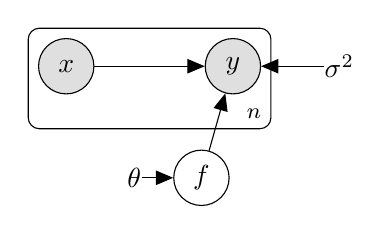
\begin{tikzpicture}
    \node[obs] (y) {$y$};
    \node[latent, below=0.7 of y, xshift=-0.4cm] (f) {$f$};
    \node[obs, left=of y, xshift=-0.4cm]  (x) {$x$};
    \node[const, right=of y, xshift=-0.2cm]  (sigma) {$\sigma^2$};
    \node[const, left=0.4 of f] (theta) {$\theta$};

    % Connect the nodes
    \edge {x, f, sigma} {y} ; %
    \edge {theta} {f} ; %

    % Plates
    \plate {yx} {(x)(y)} {$n$} ;
  \end{tikzpicture}
  \caption{Gaussian Process plate diagram.\label{fig:gp_plate} }
\end{figure}


In this model, the posterior of $f$ is available analytically, by virtue of
Gaussian-Gaussian conjugacy. Consider evaluating the function $f$ at new points
$x_{\ast}$, denoted by $f_{\ast} := f\left(x_{\ast}\right)$. The joint of $y$
and $f^{\ast}$ is
\begin{align*}
  \begin{pmatrix}
    y \\ f_{\ast}
  \end{pmatrix} &= \Gsn\left(
 \begin{pmatrix}
   0 \\ 0
 \end{pmatrix} ,
\begin{pmatrix}
  K\left(x, x\right) + \sigma^{2}I_{n} & K\left(x, x_{\ast}\right) \\
  K\left(x_{\ast}, x\right) & K\left(x_{\ast}, x_{\ast}\right)
\end{pmatrix}
  \right),
\end{align*}
which yields the posterior,
\begin{align*}
  f_{\ast} \vert y &\sim \Gsn\left(\Earg{f_{\ast} \vert y}, \Covarg{f_{\ast} \vert y}\right),
\end{align*}
where
\begin{align*}
  \Earg{f_{\ast} \vert y} &= K\left(x_{\ast}, x\right)\left(K\left(x, x\right) + \sigma^{2}I_{n}\right)^{-1}y \\
  \Covarg{f_{\ast} \vert y} &= K\left(x_{\ast}, x_{\ast}\right) - K\left(x_{\ast}, x\right)\left(K\left(x, x\right) + \sigma^{2}I_{n}\right)^{-1}K\left(x, x_{\ast}\right).
\end{align*}
Note the $n\times n$ matrix inversion in the covariance calculation. This is the
source of the $O\left(n^{3}\right)$ complexity of using standard GPs, though a
variety of fast approximations have been proposed, exploiting the sparse,
banded, or block structure often present in covariance matrices
\citep{quinonero2007approximation}.

In this computation, we have assumed the the kernel hyperparameters $\theta$ are
known\footnote{For example, in the Gaussian covariance case, this has the form
  $\theta = \left(\sigma_{f}^{2}, M\right)$}. In reality, these must be inferred
from the data. Two standard approaches are based on maximizing (1) the marginal
likelihood of $y$ and (2) the cross-validated predictive likelihood. The first
approach leverages the fact that the marginal likelihood,
\begin{align*}
  \log p\left(y \vert x; \theta\right) &= -\frac{n}{2}\log 2\pi - \log\absarg{K_{\theta}\left(x, x\right) + \sigma^{2}I_{n}} - \frac{1}{2}y^{T}\left(K_{\theta}\left(x, x\right) + \sigma^{2}I_{n}\right)^{-1}y
\end{align*}
and its gradients over $\theta$ have a closed form, and so can be optimized.

The cross-validation approach instead maximizes the average predicted log probability,
\begin{align*}
\sum_{i = 1}^{n} \log p\left(y_{i} \vert x, y_{-i}; \theta\right),
\end{align*}
which can also be found analytically, by conditioning the marginal for $y$.

%% Might be nice to give pseudocode

\subsection{Linear Dynamical Systems}
\label{subsec:linear_dynamical_systems}

Linear Dynamical System models (LDSs) treat an observed time series as a
transformation of temporally evolving latent states.
%% The basic idea reminds me of trying to swat a
%% fly. I might hear a buzzing noise, which gives some sense of where the fly is,
%% and I might know that it can't move too far too quickly, but I might only get a
%% few brief glimpses of the actual insect. The evolving latent state here is the
%% true position of the fly, while the transformation that we observe is the
%% loudness of the buzzing.
There have been many proposals that allow general transformation and state
evolution behavior \citep{hostetler1983nonlinear, wan2000unscented}, but a
fundamental starting point is the Linear-Gaussian dynamical system,
\begin{align*}
  x_{t} &= C z_{t} + \eps_{t} \\
  z_{t} &= A z_{t - 1} + \delta_{t} \\
  \eps_{t} &\sim \Gsn\left(0, R\right) \\
  \delta_{t} &\sim \Gsn\left(0, Q\right).
\end{align*}
The $z_{t}$'s are a Markov chain of latent states, while the $x_{t}$'s represent
the observed emissions from it. $A$ and $Q$ govern the dynamics of the
underlying process, while $C$ and $R$ describe the emission structure. The
associated graphical model is provided in Figure \ref{fig:lds_graphical}.

There are two conceptual components to fitting this model,
\begin{itemize}
\item Inference: Even if $\Theta = \{A, C, Q, R\}$ were known, there
  is often value in estimating the latent $z_{i}$.
\item Learning: Typically, the parameters $\Theta$ are unknown, and must
  themselves be learned from the data.
\end{itemize}

Further, inference can be approached in several different ways, depending on
problem context and constraints. Among the most common approaches are
\begin{itemize}
\item Filtering: Update beliefs of the current latent state in an online
  fashion. Quantitatively, the goal is to estimate the distribution
  $p\left(z_{t} \vert x_{1:t}\right)$.
\item Smoothing: Use the full history to estimate beliefs of latent states at
  each time. This means to compute $p\left(z_{t} \vert x_{1:T}\right)$ for each
  $t = 1, \dots, T$.
\item Forecasting: Predict the next few latent states given all observations so
  far. For example, we might be interested in $p\left(z_{t + 1} \vert
  x_{1:t}\right)$.
\end{itemize}

\begin{figure}
  \centering
  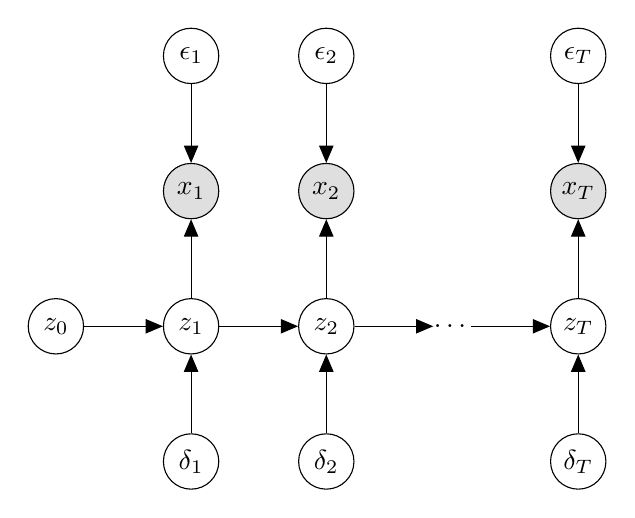
\begin{tikzpicture}
    \node[latent] (z1) {$z_{1}$};
    \node[latent, left=of z1] (z0) {$z_{0}$};
    \node[obs, above=of z1] (x1) {$x_{1}$};
    \node[latent, above=of x1] (eps1) {$\eps_{1}$};
    \node[latent, below=of z1] (delta1) {$\delta_{1}$};
    \node[latent, right=of z1] (z2) {$z_{2}$};
    \node[obs, above=of z2] (x2) {$x_{2}$};
    \node[latent, above=of x2] (eps2) {$\eps_{2}$};
    \node[latent, below=of z2] (delta2) {$\delta_{2}$};
    \node[const, right=of z2] (zdots) {$\dots$};
    \node[latent, right=of zdots] (zT) {$z_{T}$};
    \node[latent, below=of zT] (deltaT) {$\delta_{T}$};
    \node[obs, above=of zT] (xT) {$x_{T}$};
    \node[latent, above=of xT] (epsT) {$\eps_{T}$};

    % Connect the nodes
    \edge {z1} {x1} ;
    \edge {z2} {x2} ;
    \edge {z0} {z1} ;
    \edge {z1} {z2} ;
    \edge {z2} {zdots} ;
    \edge {zdots} {zT} ;
    \edge {zT} {xT} ;
    \edge {eps1} {x1} ;
    \edge {eps2} {x2} ;
    \edge {epsT} {xT} ;
    \edge {delta1} {z1} ;
    \edge {delta2} {z2} ;
    \edge {deltaT} {zT} ;
  \end{tikzpicture}
  \caption{Plate diagram corresponding to a Gaussian LDS. $z_{t}$ denotes the
    underlying Markov state sequence, while $x_t$ are observed
    emissions. \label{fig:lds_graphical} }
\end{figure}

We first describe inference in detail, before explaining how inference and
learning can be alternated to fit models on real data. Due to the
Linear-Gaussian assumption, the conditionals required by filtering and smoothing
are still Gaussian; however, their means and covariances are not immediately
apparent. It turns out that, for both filtering and smoothing, they can be
efficiently computed via dynamic programming recursions. In the literature,
these are referred to as the Kalman Filtering and Rauch-Tung-Striebel (RTS)
smoothing recursions.

Consider the filter, where the goal is the calculation of $p\left(z_{t} \vert
x_{1:t}\right)$. We will assume $z_{1} \sim \Gsn\left(0, Q\right)$. We could
alternatively fix it to a constant -- the point is that the distribution for
$z_{1}$ must be known.

For $t > 1$, define the \textit{one-step-ahead} and \textit{updated} means and
covariances by
\begin{align*}
  \mu_{t \vert t - 1} &:= \Earg{z_{t} \vert x_{1:t - 1}} \\
  \Sigma_{t \ vert t - 1} &:= \Covarg{z_{t} \vert x_{1:t - 1}} \\
  \mu_{t} &:= \Earg{z_{t} \vert x_{1:t}} \\
  \Sigma_{t} &:= \Covarg{z_{t} \vert x_{1:t}}.
\end{align*}
The means $\mu_t$ and covariances $\Sigma_{t}$ are the main quantities of
interest in filtering. The filtering algorithm is detailed in in Algorithm
\ref{alg:kalman_filter}. It can be thought of as a forwards pass through the
observed sequence, updating means and covariances along the way.

The derivation is as follows. For the predict step, use the tower property and
the law of total variance,
\begin{align*}
  \Earg{z_{t} \vert x_{1:t - 1}} &= \Earg{\Earg{z_{t} \vert z_{t - 1}, x_{1:t - 1}}} \\
  & = \Earg{Az_{t - 1}\vert x_{1:t - 1}} \\
  &= A\mu_{t - 1}, \\
  \Covarg{z_{t} \vert x_{1:t - 1}} &= \Covarg{\Earg{z_{t} \vert z_{t - 1}, x_{1:t - 1}}} + \Earg{\Covarg{z_{t} \vert z_{t - 1}, x_{1:t - 1}}} \\
  &= \Covarg{Az_{t - 1} \vert z_{t - 1}, x_{1:t - 1}} + \Earg{Q} \\
  &= A\Sigma_{t - 1}A^{T} + Q.
\end{align*}
For the update step, use Gaussian conjugacy to obtain the required means and
covariances and the matrix inversion lemma to express them more concisely.
More precisely,
\begin{align*}
  p\left(z_{t} \vert x_{1:t}\right) \propto p\left(x_{t} \vert z_{t}\right)p\left(z_{t} \vert x_{1:\left(t - 1\right)}\right),
\end{align*}
and both densities on the right are Gaussian -- the first is the likelihood of
the observed $x_{t}$ while the second is the predict-step density derived above.
By Bayes' rule, the posterior is Gaussian with increased precision,
\begin{align}
  \label{eq:sigma_t_inv}
\Sigma_{t}^{-1} &= \Sigma_{t \vert t - 1}^{-1} + C^{T}R^{-1}C
\end{align}
and shrunken mean,
\begin{align}
  \label{eq:mu_t}
\mu_{t} &= \Sigma_{t}CR^{-1}x_{t} + \Sigma_{t}\Sigma_{t \vert t - 1}^{-1} \mu_{t \vert t - 1}.
\end{align}

Recall the matrix inversion lemma,
\begin{align*}
\left(A + UCV\right)^{-1} &= A^{-1} + A^{-1}U\left(C^{-1} + VA^{-1}U\right)^{-1}VA^{-1},
\end{align*}
and apply it to equation \ref{eq:sigma_t_inv} to find
\begin{align*}
  \Sigma_{t} &= \Sigma_{t \vert t - 1} - \Sigma_{t \vert t - 1}C^T\left(R + C \Sigma_{t \vert t - 1}C^{T}\right)^{-1}C\Sigma_{t \vert t - 1} \\
  &= \left(I - K_{t}C\right)\Sigma_{t \vert t - 1},
\end{align*}
according to the definition of $K_{t}$ in Algorithm
\ref{alg:kalman_filter}.

Substituting this expression, we can simplify equation \ref{eq:mu_t},
\begin{align*}
  \mu_{t} &= \left(I - K_{t} C\right)\Sigma_{t \vert t - 1}\left(C R^{-1}x_{t} + \Sigma_{t \vert t - 1}^{-1} \mu_{t \vert t - 1}\right) \\
  &= \left(I - K_{t}C\right)\mu_{t \vert t - 1} + \left(I - K_{t} C\right)\Sigma_{t \vert t - 1}C R^{-1} x_{t} \\
  &= \mu_{t \vert t - 1} + K_{t}\left(x_{t} - C\mu_{t \vert t- 1}\right),
\end{align*}
where for the simplification on the second half of the second line,
\begin{align*}
  \left(I - K_{t}C\right)\Sigma_{t \vert t - 1} C R^{-1} x_{t} &= \left(I - \left(\Sigma_{t \vert t - 1}^{-1} + C^{T} R C\right)^{-1}C^{T}R^{-1}C\right)\Sigma_{t \vert t - 1}C R^{-1} x_{t} \\
  &= K_{t}x_{t},
\end{align*}
we again used the matrix inversion lemma.

\begin{algorithm}
   \caption{The Kalman filtering predict-update recursions.}
   \label{alg:kalman_filter}
\begin{algorithmic}
  \STATE {\bfseries Input:} Model parameters $\Theta = \{A, C, Q, R\}$ and
    observed sequence $x_{1:T}$.
    \STATE $\mu_{0} \leftarrow 0, \Sigma_{0} \leftarrow Q$ \hfill initialize distribution of
    $z_{0}$.
    \FOR{$t = 1 \dots T$}
    \STATE $\mu_{t \vert t - 1} \leftarrow A\mu_{t - 1}$ \hfill predict step
    \STATE $\Sigma_{t \vert t - 1} \leftarrow A \Sigma_{t - 1} A^{T} + Q$
    \STATE $\mu_{t} \leftarrow \mu_{t \vert t - 1} + K_{t}\left(x_{t} - C\mu_{t \vert t - 1}\right)$ \hfill update step
    \STATE $\Sigma_{t} \leftarrow \left(I - K_{t}C\right)\Sigma_{t \vert t - 1}$
    \STATE where $K_{t} \leftarrow \left(\Sigma_{t \vert t - 1}^{-1} + C^{T}R C\right)^{-1} C^{T}R^{-1}$
    \ENDFOR
    \STATE {\bfseries Output:} Filtered means and covariances $\left(\mu_{t},
    \Sigma_{t}\right)_{t = 1}^{T}$.
\end{algorithmic}
\end{algorithm}
While the Kalman filter makes a forwards pass over the observations to estimate
the latent state means and covariances as data are made available, the RTS
smoother can be understood as a pair of forwards-backwards sweeps that propogate
information from all observations to the latent state estimates obtained by
filtering. Define the quantities,
\begin{align*}
\mu_{t \vert T} &= \Earg{z_{t} \vert x_{1:T}} \\
\Sigma_{t \vert T} &= \Covarg{z_{t} \vert x_{1:T}},
\end{align*}
which completely determine the smoothed distributions $p\left(z_{t} \vert
x_{1:T}\right)$ of interest. The forwards pass in RTS smoothing is identical to
the Kalman filter, and pseudocode for the backwards pass is provided in
Algorithm \ref{alg:kalman_smoother}.

\begin{algorithm}
   \caption{The Kalman smoothing backwards pass.}
   \label{alg:kalman_smoother}
\begin{algorithmic}
  \STATE {\bfseries Input:} Model parameters $\Theta = \{A, C, Q, R\}$,
    observed sequence $x_{1:T}$, and filtering quantities $\left(\mu_{t},
    \Sigma_{t}, \mu_{t \vert t - 1}, \Sigma_{t \vert t - 1}\right)$
    \STATE $\mu_{T \vert T} \leftarrow \mu_{T}, \Sigma_{T \vert T} \leftarrow
    \Sigma_{T}$ \hfill initialize distribution of $z_{T}$ from the Kalman
    filter.
    \FOR{$t = T - 1 \dots 1$}
    \STATE $\mu_{t \vert T} \leftarrow \mu_{t} + J_{t}\left(\mu_{t + 1 \vert T} - \mu_{t + 1 \vert t}\right)$
    \STATE $\Sigma_{t \vert T} \leftarrow \Sigma_{t} + J_{t}\left(\Sigma_{t + 1 \vert T} - \Sigma_{t + 1 \vert t}\right)J_{t}^{T}$
    \STATE where $J_{t} \leftarrow \Sigma_{t \vert t}A_{t + 1}^{T} \Sigma_{t + 1\vert t}^{-1}$
    \ENDFOR
    \STATE {\bfseries Output:} Smoothed means and covariances $\left(\mu_{t \vert T},
    \Sigma_{t \vert T}\right)_{t = 1}^{T}$.
\end{algorithmic}
\end{algorithm}

To see why this update works, first consider the joint behavior of neighboring
times,

\begin{align*}
   \left(z_{t}, z_{t + 1}\right) \vert x_{1:t} &\sim \Gsn\left(
\begin{pmatrix}
  \mu_{t \vert t} \\
  \mu_{t + 1 \vert t}
\end{pmatrix},
\begin{pmatrix}
  \Sigma_{t \vert t} & \Sigma_{t} A^{T} \\
  A \Sigma_{t} & \Sigma_{t + 1 \vert t}
\end{pmatrix}\right),
\end{align*}
because
\begin{align*}
  \Covarg{z_{t}, z_{t + 1} \vert x_{1:t}} &= \Covarg{z_{t}, Az_{t} + \eps_{t + 1} \vert x_{1:t}} \\
  &= \Sigma_{t}A^{T}.
\end{align*}

Conditioning, we obtain
\begin{align*}
  z_{t} \vert z_{t + 1}, x_{1:t} &\sim \Gsn\left(
  z_{t} \vert \mu_{t \vert t} + J_{t}\left(z_{t + 1} - \mu_{t + 1 \vert t}\right),
  \Sigma_{t \vert t} - J_{t} \Sigma_{t + 1 \vert t} J_{t}^{T}
  \right).
\end{align*}
Since $x_{t}$ is independent of $x_{(t + 1): T}$ conditional on $z_{t + 1}$,
this is enough to compute the full smoothed means and covariances. By the tower
property,
\begin{align*}
  \mu_{t \vert T} &= \Earg{z_{t} \vert x_{1:T}} \\
  &= \Earg{\Earg{z_{t} \vert z_{t + 1}, x_{1 : T}} \vert x_{1:T}} \\
  &= \Earg{\Earg{z_{t} \vert z_{t + 1}, x_{1:t}} \vert x_{1:T}} \\
  &= \mu_{t \vert t} + J_{t}\left(\mu_{t + 1 \vert T} - \mu_{t + 1 \vert t}\right)
\end{align*}
and similarly by the law of total covariance,
\begin{align*}
  \Sigma_{t\vert T} &= \Covarg{z_{t} \vert x_{1:T}} \\
  &= \Covarg{\Earg{z_{t} \vert z_{t + 1}, x_{1:T}}} + \Earg{\Covarg{z_{t} \vert z_{t + 1}, x_{1:T}}} \\
  &= \Covarg{\Earg{z_{t} \vert z_{t + 1}, x_{1:t}}} + \Earg{\Covarg{z_{t} \vert z_{t + 1}, x_{1:t}}} \\
  &= \Sigma_{t \vert t} + J_{t}\left(\Sigma_{t + 1 \vert T} - \Sigma_{t + 1 \vert t}\right) J_{t}^{T}
\end{align*}

\subsubsection{Zero-inflation in dynamical systems}
\label{subsubsec:zero_inflation_dynamical}

After transformations, many microbiome data sets can be viewed as a mixture
between a continuous, nonnegative component and a spike at 0. Such data has a
rich history in statistics, and has been approached using hurdle and tobit
modeling ideas \citep{min2002modeling}. In this section, we take a detour from
our review of standard temporal modeling methods, to describe a variation of the
standard LDS, called the dynamic tobit model (DTM), that is designed for the
zero-spiked density situation.

The basic idea of the DTM is to truncate an LDS below some threshold, so that
the continuous positive data correspond to excursions of the LDS above some
threshold, while the zeros correspond to parts of the path below the threshold.
That is, the observed data $y_t$ are modeled according to
\begin{align*}
  y_{t} \vert x_t, \tau &= \left(x_t - \tau\right)\indic{x_t > \tau}  \\
  x_t \vert z_t &\sim \Gsn\left(x_t \vert C z_{t}, R\right) \\
  z_t \vert z_{t - 1} &\sim \Gsn\left(z_t \vert A z_{t - 1}, Q\right).
\end{align*}
Note that last two equations are exactly those defining an LDS, but that $x_t,
z_t$, and $\tau$ are all unobserved data in this setting. As before, $A, C, R,
Q$ are model parameters to be learned.

There are several approaches to inference in this model, including particle
filtering \citep{doucet2000rao}, Monte Carlo EM \citep{manrique1998simulation},
and Gibbs sampling \citep{de1997scan, wei1999bayesian}. In many of these
approaches, recursions like those used in the Kalman filter can be used to
perform efficient sampling and estimation.

To give an example, we review one method here, the scan sampler of
\cite{de1997scan}. For simplicity, we will assume that $\tau$ is known and
equal to zero. The scan sampler iterates filter and smoother-type calculations
for $x_t$, at each step sampling from a distribution with mean $\Earg{x_t \vert
  x_{-t}}$ and variance $\Covarg{x_t \vert x_{-t}}$. In the Gaussian case
presented above, this provides the exact posterior, though \cite{de1997scan}
describe its utility for general exponential families.

To initialize the scan sampler for the DTM, first set $x_t = y_t$ for all $t$,
then perform a Kalman filter and smoother step. This gives estimates of the
following quantities, using notation analogous to that in the previous section,
\begin{align*}
  \mu_{t \vert t - 1}^{x} &= \Earg{x_t \vert x_{0:\left(t - 1\right)}} \\
  \mu_{t \vert t - 1}^{z} &= \Earg{z_t \vert z_{0:\left(t - 1\right)}} \\
  \Sigma_{t \vert t - 1}^{x} &= \Covarg{x_t \vert x_{0:\left(t - 1\right)}} \\
  \Sigma_{t \vert t - 1}^{z} &= \Covarg{z_t \vert z_{0 : \left(t - 1\right)}}.
\end{align*}

The idea of the scan sampler is to iteratively compute $M_t$ and $u_t$ such that
\begin{align*}
  M_t^{-1} &= \Covarg{x_t \vert x_{-t}} \\
  M_t^{-1}u_t &= x_t - \Earg{x_t \vert x_{-t}}
\end{align*}
so that sampling can cycle forwards and backwards through coordinates of
$\left(x_t\right)$, drawing $x_t^{\prime} \sim \Gsn\left(\Earg{x_t \vert
  x_{-t}}, \Covarg{x_t \vert x_{-t}}\right) = \Gsn\left(x_t - M_t^{-1}u_t,
M_t^{-1}\right)$. Details of the derivation can be found in \citep{de1997scan},
we simply describe the updates necessary to compute $M_t$ and $u_t$, along with
an example application. In an initial backwards pass through the data, we
compute
\begin{align*}
  u_t &= \left(\Sigma_{t \vert t - 1}^{x}\right)^{-1}\mu_{t \vert t - 1}^{x} - K_t^{T}r_t \\
  M_t &= \left(\Sigma_{t \vert t - 1}^{x}\right)^{-1} + K_t^{T} N_t K_t,
\end{align*}
where $K_t$ is the Kalman gain matrix at time $t$ and
\begin{align*}
  r_t &= C^T u_{t + 1} + A^{T}r_{t + 1} \\
  N_t &= C^{T} \Sigma_{t + 1 \vert t}C + L_{t + 1}^{T}N_{t + 1}L_{t + 1}.
\end{align*}
The $M_t$ remain fixed after this initial scan, and sampling proceeds only by
cycling through the $u_t$. During the forwards scan, $u_t$ is updated according
to
\begin{align*}
  u_t \xleftarrow u_t - \left(\Sigma_{t \vert -t}^{x} C - K_t^{T}N_t\right) b_t \\
  b_{t + 1} &= L_{t} b_t - K_t M_t^{-1}u_t
\end{align*}
where $L_t = A - K_t C$, while for backwards scans, the analogous updates are
\begin{align*}
  u_t \xleftarrow u_t - K_t^{T} b_t \\
  b_{t - 1} &= L_t^T b_t - C_t^{T}M_t^{-1}u_t.
\end{align*}
Each time a $u_t$ is computed, it is used to update the unobserved $x_t$ by
sampling from $\Gsn\left(x_t - M_t^{-1}u_t, M_t^{-1}\right)$.

Code implementing these updates is available at
\url{https://github.com/krisrs1128/tsc_microbiome/tree/master/src/scan}. We have
also provided an example application to a real microbial abundance time series,
whose results are provided in Figure \ref{fig:abt_scan}.

\begin{figure}
  \centering
  \includegraphics[width=\textwidth]{figure/regime_detection/abt_scan}
  \caption{Posterior samples from a DTM applied to a bacterial abundance time
    series, obtained using the scan sampler. We fix $A, C, Q, R$ for the
    dynamical system component to arbitrary, stable values. Black points
    represent observed data, while blue points are draws from the scan sampler
    posterior. The blue line is a loess smooth of the posterior samples for
    $x_t$.
    \label{fig:abt_scan}}
\end{figure}

\section{Temporal mixture models}
\label{sec:temporal_mixture_models}

In the models considered in Section \ref{sec:smooth_temporal_models}, all
time windows exhibit comparable behavior. From the problem description of
Section \ref{sec:problem_description} however, we would expect changes in the
behavior of the system during different temporal regimes. In this section, we
describe probabilistic models that generate this sort of behavior. The unifying
probabilistic ``trick'' that helps accomplish this goal is the introduction of
latent variables specying which regime the system is in at any given timepoint.

\subsection{Hidden Markov Models}
\label{subsec:hmms}

The idea behind Hidden Markov Models (HMMs) is similar to that of LDSs, with the
exception that the $z_{t}$ are no longer thought of as continuous latent
variables. Instead, each $z_{t}$ is assigned one of a few discrete states, which
transition between modeled states according to a Markov chain.

An informal analogy is how I choose to listen to different music tracks. For a
few days, I might be mostly listening to sonatas by Beethoven and Schubert,
because I'm in a latent state that prefers German piano sonatas. I might be more
likely to transition from here to French chamber music than, say, LA punk. So,
my underlying style preferences evolve according to a Markov chain $z_{t}$,
which is in turn reflected by the actual tracks $x_{t}$ that I listen to.

More formally, we suppose $z_{1} \sim \pi_{1}$ comes from some initial
distribution $\pi_{1} \in \simplex^{K - 1}$ and has some $K \times K$ transition
probability matrix $P$ whose rows lie in $\simplex^{K - 1}$, the $K - 1$
dimensional simplex. Conditional on $z_{t}$, $x_{t}$ is emitted according to the
density $p_{\theta_{z_{t}}}\left(x\right)$, one of $K$ emission densities
$p_{\theta_{1}}\left(x\right), \dots, p_{\theta_{K}}\left(x\right)$. Concisely,
\begin{align*}
  x_{t} \vert z_{t} &\sim p_{\theta_{z_{t}}} \\
  z_{t} \vert z_{t - 1} &\sim P_{z_{t - 1}} \text{ for } t > 1 \\
  z_{1} &\sim \pi_{1}
\end{align*}
As in LDSs, fitting this model can be broken into inference and learning steps,
which estimate the distributions of the $z_{t}$ conditional on observed data and
which fit the model parameters $\{P, \pi, \theta_{1}, \dots, \theta_{K}\}$,
respectively. Alternating these two steps optimizes the expected complete data
loglikelihood in an EM algorithm.

The $E$-step, which infers latent states, is referred to as the
forwards-backwards algorithm. This procedure parallels the Kalman filter
(forwards) and smoother (backwards) algorithm for inference in LDSs. First, we
find a simple expression for the analog of the filtered densities, based on the
Markov property for the $z_{t}$'s,
\begin{align*}
  p\left(z_{t} \vert x_{1:t}\right) &\propto p\left(x_{t} \vert z_{t}, x_{1:t - 1}\right) p\left(z_{t} \vert x_{1:t - 1}\right) \\
  &= p\left(x_{t} \vert z_{t}\right) p\left(z_{t} \vert x_{1:t - 1}\right) \\
  &= p_{\theta_{z_{t}}}\left(x_{t}\right)p\left(z_{t} \vert x_{1:t - 1}\right).
\end{align*}
The first term is known by assumption, while the second can be computed from the
previous filtered probabilities,
\begin{align*}
  p\left(z_{t} \vert x_{1:t - 1}\right) &= \sum_{k = 1}^{K} p\left(z_{t} \vert z_{t - 1} = k\right)p\left(z_{t - 1} = k \vert x_{1:t - 1} \right).
\end{align*}

The forwards pass of the Forwards-Backwards algorithm alternates these two steps
(``update'' and ``predict''), after initializing $p\left(z_{1}\right) =
\pi_{1}$, as described in Algorithm \ref{alg:hmm_forwards}.

\begin{algorithm}
   \caption{Safe log-sum-exp}
   \label{alg:normalize_log}
   \begin{algorithmic}
     \STATE {\bfseries Input:} $x \in \reals^{n}$
     \STATE $m \leftarrow \max\left(x\right)$
     \STATE {\bfseries Output:} $\text{lse}\left(x\right) \leftarrow x - \left(m + \log\left(\sum\exp{x_{i} - m}\right)\right)$
   \end{algorithmic}
\end{algorithm}

\begin{algorithm}
   \caption{Forwards pass for HMM Inference}
   \label{alg:hmm_forwards}
\begin{algorithmic}
  \STATE {\bfseries Input:} Model parameters $\{\pi_{1}, P, \theta_1, \dots, \theta_K\}$,
  observed sequence $x_{1:T}$
  \STATE $\log \tilde{p}\left(z_{1}\vert x_{1}\right) \leftarrow
  \log\pi_{1} + \begin{pmatrix} \log p_{\theta_{1}}\left(x_{1}\right) \\ \vdots \\ \log p_{\theta_{k}}\left(x_{1}\right) \end{pmatrix}$ \hfill initialize distribution of $z_{1}$
  \STATE $\log p\left(z_{1} \vert x_{1}\right) \leftarrow \log \tilde{p}\left(z_{t} \vert x_{1}\right) - \text{lse}\left(\log \tilde{p}\left(z_{t} \vert x_{1}\right)\right)$\hfill Normalize with Algorithm \ref{alg:normalize_log}
  \FOR{$t = 2 \dots T$}
  \STATE $\log \tilde{p}\left(z_{t} \vert x_{1:t}\right) \leftarrow P \exp{\log p\left(z_{t - 1} \vert x_{1:t - 1}\right)} + \begin{pmatrix}  \log p_{\theta_{1}}\left(x_{t}\right) \\ \vdots \\ \log p_{\theta_{K}}\left(x_{t}\right) \end{pmatrix}$
  \STATE $\log p\left(z_{1} \vert x_{1:t}\right) \leftarrow \log \tilde{p}\left(z_{t} \vert x_{1:t}\right) - \text{lse}\left(\log \tilde{p}\left(z_{t} \vert x_{1:t}\right)\right)$\hfill
  \ENDFOR
  \STATE {\bfseries Output:} Filtered log densities $\log p\left(z_{t} \vert x_{1:t}\right)$.
\end{algorithmic}
\end{algorithm}

\begin{algorithm}
  \begin{algorithmic}
   \caption{Backwards pass for HMM Inference}
   \label{alg:hmm_backwards}
   \STATE {\bfseries Input:} Model parameters $\{\pi_{1}, P, \theta_1, \dots, \theta_k\}$, observed sequence $x_{1:T}$
   \STATE $\log p\left(x_{T + 1} \vert z_T\right) \leftarrow 0_{K}$ \hfill Initialize messages.
   \FOR{$t = T  - 1\dots 1$}
   \FOR{$k = 1 \dots K$}
   \STATE $\log p\left(x_{\left(t + 1\right): T} \vert z_{t} = k\right) \leftarrow \text{lse}\left(\log p\left(x_{\left(t + 2\right):T} \vert z_{t + 1}\right) + \begin{pmatrix} \log p_{\theta_{1}}\left(x_{t}\right) \\ \vdots \\ p_{\theta_{K}}\left(x_t\right)\end{pmatrix} + \log P_{k}\right)$
   \ENDFOR
   \ENDFOR
   \STATE {\bfseries Output:} Smoothed densities $\log p\left(z_{t} \vert x_{1:T}\right)$.
  \end{algorithmic}
\end{algorithm}

The backwards pass computes the analog of the smoothed densities, based on the
observation\footnote{This is the same observation used in the derivation of the
  Kalman smoother.} that $x_{t}$ is independent of the future conditional on
$z_{t + 1}$,
\begin{align*}
  p\left(z_{t} \vert x_{1:T}\right) &\propto p\left(x_{t + 1:T} \vert z_{t}\right) p\left(z_{t} \vert x_{1:t}\right).
\end{align*}
The second term on the right hand side is available from the forwards pass. The
first term is computed during the backwards pass, which initializes $p\left(x_{T
  + 1} \vert z_{T}\right) = 1$ and then accumulates the ``future observation''
densities from right to left,
\begin{align*}
  p\left(x_{t + 1: T} \vert z_{t}\right) &= \sum_{k = 1}^{K} p\left(z_{t + 1} = k, x_{t + 1 : T} \vert z_{t}\right) \\
  &= \sum_{k = 1}^{K} p\left(x_{t + 2: T}\vert z_{t + 1} = k, x_{t + 1}, z_{t}\right) p\left(z_{t + 1} = k, x_{t + 1} \vert z_{t}\right) \\
  &= \sum_{k = 1}^{K} p\left(x_{t + 2:T}\vert z_{t + 1} = k\right)p_{\theta_{z_{t + 1}}}\left(x_{t + 1}\right) P_{z_{t}, k}.
\end{align*}
The backwards pass is summarized in Algorithm \ref{alg:hmm_backwards}.

In the M-step, the parameters $\left(\theta_{k}\right)$, $\pi_0$ and
$P_{k, k^{\prime}}$ must be learned. Estimation of the per-regime parameters
can be done separately for each $k$. For example, if HMM has Gaussian emissions,
$p_{\theta_{k}}\left(x_{t}\right) = \Gsn\left(x_{t} \vert \mu_{k},
\Sigma_{k}\right)$, then
\begin{align*}
  \hat{\mu}_{k} &= \frac{\sum_{t = 1}^{T} \indic{z_{t} = k}x_{t}}{\sum_{t = 1}^{T}\indic{z_{t} = k}} \\
  \hat{\Sigma}_{k} &= \frac{\sum_{t = 1}^{T} \indic{z_{t} = k}\left(x_{t} - \hat{\mu}_{k}\right)\left(x_{t} - \hat{\mu}_{k}\right)^{T}}
      {\sum_{t = 1}^{T} \indic{z_{t} = k}},
\end{align*}
while, regardless of the emission structure, the Markov chain parameters can be
estimated via
\begin{align*}
  \hat{\pi}_{k, k^{\prime}} &= \frac{\sum_{t = 1}^{T} \indic{z_{t} = k, z_{t + 1} = k^{\prime}}}{\sum_{t = 1}^{T} \indic{z_{t} = k}}.
\end{align*}

\subsubsection{Example}
\label{subsubsec:hmm_example}

In the context of regime detection in the microbiome, we imagine a few
underlying states shared across all bacteria, with means ranging from high abundance to
complete absence. Within each species, states evolve independently according to
a Markov chain. Note that, while we do share across species when estimating
underlying parameters $\left(\theta_{k}\right)$, we do not tie together latent
indicators $z_{it}$ across species. Specifically, we use a DAG that factors
across all species -- given $\theta$, all species abundances follow independent
HMMs.

Therefore, in the $E$-step (the forwards-backwards algorithm) the $z_{it}$ can
be estimated in parallel across all species. The $M$-step is modified so that
mixture component parameters and transition probabilities are estimated
simultaneously across all species, for example, the new mean update for cluster
$k$ in an HMM with Gaussian emissions becomes
\begin{align*}
\hat{\mu}_{k} &= \frac{\sum_{i = 1}^{n}\sum_{t = 1}^{T} \indic{z_{t} = k}x_{it}}{\sum_{i = 1}^{n}\sum_{t = 1}^{T} \indic{z_{it} = k}}.
\end{align*}
We employ this approach on the antibiotics data described in Section
\ref{subsubcart_example}. The results are summarized in Figure
\ref{fig:hmm_mode} and Supplementary Figure \ref{fig:hmm_probs}, which display
the modes and raw probabilities of the smoothed probabilities $p\left(z_{it}
\vert x_{i, 1:T}\right)$ after applying EM. As in Figure
\ref{fig:centroid-euclidean-conditional} and its counterparts made through
hierarchical clustering, rows correspond to individual species, while columns
are samples sorted by time. The three main panels are the three subjects in the
study. Rows $i$ are ordered according to a hierarchical clustering on Euclidean
distances between sequences $\left(\hat{z}_{i1}, \dots, \hat{z}_{iT}\right)$,
where $\hat{z}_{it} = \arg \max_{k} p\left(z_{it} = k \vert x_{1:T}\right)$. The
intensity of the shading of each cell corresponds to the average value
$\hat{\mu}_{k}$ for that mode.

We can think of Figure \ref{fig:hmm_mode} as a smoothed version of the raw
heatmaps made through hierarchical clustering. By coarsening the raw values into
cluster centers, certain patterns are more easily visible. For example, in
addition to effect of the two antibiotics time courses across all subjects, we
note that

\begin{itemize}
\item The effect of the first antibiotic time courses is more prolonged in
  subject F, and in some cases species disappear for most of the remainder of
  the experiment. Some of these species seem to have also disappeared from
  subject D, but most others recovered in both subjects D and E.
\item The phenomenon in which some species become \textit{more} abundant during
  the time courses -- presumably filling in newly emptied niches -- is stronger
  in subject E than the others. Further, some species that exhibit this behavior
  in subject E respond differently within subjects D and F, becoming less
  abundant rather than more.
\end{itemize}

Note that, while smoothing makes the antibiotic effect clearer among moderately
and highly abundant species, variation among rarer species, to which all
timepoints are assigned to the rare abundance state, is obscured. This could be
remedied by increasing $K$, at the cost of increasing the complexity of
interpretation for abundant species.

Instead of displaying the sequence of modes $\hat{z}_{it}$, Supplemental Figure
\ref{fig:hmm_probs} provides the individual probabilities $p\left(z_{it} = k
\vert x_{1:T}\right)$ across $k$. The vertical panels distinguish between
different $k$, while transparency represents the size of the probability --
smaller probabilities are more transparent. The colors are associated with
centroid means, as before. In this application, most probabilities seem near
one, so this view adds little to that in Figure \ref{fig:hmm_mode}. However,
this does suggest the possibility of overfitting, which we address by
introducing priors on $\Theta$ in Section \ref{sec:sticky_hmms}.

The estimated transition probabilities between states, ordered in terms of
increasing $\hat{\mu}_{k}$, are displayed below.
\begin{verbatim}
      1     2     3     4
1 0.810 0.159 0.028 0.003
2 0.389 0.527 0.083 0.002
3 0.077 0.094 0.810 0.019
4 0.027 0.007 0.056 0.910
\end{verbatim}
Unsurprisingly, most transitions remain in the same state, and any departures
are generally restricted to states with similar $\hat{\mu}_{k}$s. Generally,
there appear to be more transitions downwards than upwards, and the sum of
transitions into state 1 is higher than the sums for the rest. This can likely
be attributed to the antibiotic effect, which reduces abundances of species that
recover at differential rates.

As in Figure \ref{fig:centroid-euclidean-conditional}, the primary drawback of
this display is the difficulty in linking observed species trajectories to
species or taxonomic detail. To easily link the smoothed HMM estimates to raw
time series values and species descriptions would require either splitting the
view across taxonomies or introducing interactivity.

\begin{figure}
  \centering
  \includegraphics[width=\textwidth]{figure/regime_detection/hmm_mode}
  \caption{The modal sequences according to the HMM estimated through
    EM. \label{fig:hmm_mode} }
\end{figure}

\subsubsection{Sticky HMMs}
\label{sec:sticky_hmms}

Sticky HMMs are an extension of ordinary HMMs designed to induce additional
``stickiness'' in state transitions -- states should be encouraged to remain
unchanged over longer stretches of time. To practically implement this basic
idea, a Bayesian view is useful, and we describe inference in detail. An
application to the antibiotics data follows this explanation.

Consider the standard Bayesian HMM, which places $\Dir\left(\alpha\right)$
priors on the rows of the transition probability matrix $P_{1}, \dots, P_{K}$
and conjugate priors on $\Theta$. The main idea of the sticky HMM is to
introduce a ``stickiness'' parameter $\kappa$ to the Dirichlet
prior\footnote{Here, $e_{k} := \left(0, \dots, 0, 1, 0, \dots, 0\right)$ is the
  vector with a $1$ in the $k^{th}$ coordinate and zeros everywhere else.}:
$P_{k} \sim \Dir\left(P_{k} \vert \alpha + \kappa e_{k}\right)$. This means that
draws from the prior on $P$ will have larger weight along the diagonal,
depending on the size of $\kappa$, and since diagonal elements correspond to
self-transitions, chains drawn from the prior will be ``sticky.''

To draw samples from $p\left(\left(z_{it}\right), P, \Theta \vert
\left(x_{it}\right)\right)$, we consider a block Gibbs sampler that parallels EM
\citep{fruhwirth2006finite}. In place of the $E$-step, we draw from the
conditional $p\left(\left(z_{it}\right) \vert \left(x_{it}\right), P,
\Theta\right)$ using a variation of the forwards-backwards algorithm, and in
place of the $M$-step, we draw from $p\left(\Theta, \vert P,
\left(z_{it}\right), \left(x_{it}\right)\right)$ and $p\left(P \vert \Theta,
\left(z_{it}\right), \left(x_{it}\right)\right)$. We detail this below,
following the derivation of \citep{fox2009bayesian}.

First consider sampling $p\left(\left(z_{it}\right) \vert \left(x_{it}\right),
P, \Theta\right)$. Since each sequence is independent of all others, given
$\Theta$, we can sample the $z_{it}$ separately across each $i$, so for the
explanation below, we drop this subscript. By the DAG structure of the HMM, the
probability a single sequence can be decomposed according to
\begin{align}
  \label{eq:sticky_block_z}
  p\left(z_{1:T} \vert x_{1:T}, \Theta, \pi, P\right) &= p\left(z_{1} \vert x_{1:T}, \Theta, \pi, P\right) \prod_{t = 2}^{T} p\left(z_{t} \vert z_{t - 1}, x_{1:T}, \Theta, \pi, P\right).
\end{align}
If we could calculate each of these individual probabilities, then one mechanism
for sampling the entire sequence $z_{1:T}$ would be to first sample $z_{1}$,
then sample $z_{2}$ given $z_{1}$, etc. Note that the first term has a different
structure than the rest (it doesn't depend on any previous $z_{t}$), so we
analyze it first,
\begin{align*}
  p\left(z_{1} \vert x_{1:T}, \Theta, \pi, P\right) &\propto p\left(z_{1} \vert \Theta, \pi, P\right) p\left(x_{1} \vert z_{1}, \Theta, \pi, P\right) p\left(x_{2:T} \vert z_{1}, \Theta, \pi, P\right) \\
  &\propto \pi_{z_{1}} p\left(x_{1} \vert \theta_{z_{1}}\right) p\left(x_{2:T} \vert z_{1}, \Theta, \pi, P\right)
\end{align*}
where we used the fact that $x_{1} \independent x_{2:T} \vert z_{1}$. The first
two terms are easy to sample, and we will show below that terms of the form
$p\left(x_{t + 1:T} \vert z_{t}, \Theta, \pi, P\right)$ can be calculated
efficiently using a backwards-pass type recursion.

Consider now the terms in the product of equation \ref{eq:sticky_block_z}. By
Bayes rule,
\begin{align*}
  p\left(z_{t} \vert z_{t - 1}, x_{1:T}, \Theta, \pi, P\right) &\propto p\left(x_{1:t - 1} \vert z_{t - 1}, z_{t}, \Theta, \pi, P\right)
  p\left(x_{t} \vert z_{t}, \Theta, \pi, P\right)
  p\left(x_{t + 1 : T} \vert z_{t}, \Theta, \pi, P\right) \\
  &\propto p\left(x_{1:t - 1} \vert z_{t - 1}, z_t, \Theta, \pi, P\right) p\left(x_t \vert \theta_{z_t}\right) p\left(x_{t + 1 : T}\vert z_{t}, \Theta, \pi, P\right).
\end{align*}
The second term is a likelihood, and the third will be calculated by the
backwards-pass. Note that the first term can be further reduced to
\begin{align*}
  p\left(x_{1:t - 1} \vert z_{t - 1}, z_t, \Theta, \pi, P\right) &\propto p\left(z_{t} \vert x_{1:t - 1}, z_{t - 1}, \Theta, \pi, P\right)p\left(x_{1:t - 1} \vert z_{t - 1}, \Theta, \pi, P\right) \\
  &\propto p\left(z_{t} \vert z_{t - 1}, \Theta, \pi, P\right) \\
  &= P_{z_{t - 1}, z_{t}},
\end{align*}
since we care only about the terms involving $z_{t}$, as we are sampling
$p\left(z_{t} \vert z_{t - 1}, x_{1:T}, \Theta, \pi, P\right)$.

We next describe how to compute the terms $p\left(x_{t + 1:T} \vert z_t, \Theta,
\pi, P\right)$ efficiently, as promised above. Consider storing these terms in a
$T \times K$ matrix, whose $tk^{th}$ element is $p\left(x_{t:T} \vert z_{t - 1} =
k, \Theta, \pi, P\right)$. The bottom row is initialized according to
\begin{align*}
 p\left(x_T \vert z_{T - 1}, \Theta, \pi, P\right)  &= \sum_{z_{T} = 1}^{K} p\left(x_{T} \vert \theta_{z_{T}}\right) P_{z_{T - 1}, z_{T}}.
\end{align*}
Then the recursion computes the $t^{th}$ row from the $t + 1^{st}$ according to
\begin{align*}
  p\left(x_{t + 1:T} \vert z_t, \Theta, \pi, P\right) &= \sum_{z_{t + 1} = 1}^{K} p\left(x_{t + 1 : T} \vert z_{t}, z_{t + 1} \Theta, \pi, P\right) P_{z_{t}, z_{t + 1}} \\
  &= \sum_{z_{t + 1} = 1}^{K} p\left(x_{t + 1} \vert \theta_{z_{t + 1}}\right) p\left(x_{t + 2 : T} \vert z_{t + 1}, \Theta, \pi, P\right) P_{z_{t}, z_{t + 1}}.
\end{align*}

Next consider sampling from the conditional $p\left(P \vert \left(x_{it}\right),
\left(z_{it}\right), \Theta\right)$ of transition probabilities between the $K$
states. The main observation is that we can use Dirichlet-Multinomial conjugacy
jointly across all sequences. That is, defining
\begin{align*}
 n_{k \cdot} &:= \begin{pmatrix} \sum_{i = 1}^{n} \sum_{t = 1}^{T - 1} \indic{z_{it} = k, z_{i,t + 1} = 1} \\ \vdots \\ \sum_{i = 1}^{n} \sum_{t = 1}^{T - 1} \indic{z_{it} = k, z_{i,t + 1} = K} \end{pmatrix},
\end{align*}
we have
\begin{align*}
n_{k\cdot} &\sim \Mult\left(n_{k\cdot} \vert \sum_{i = 1}^{n} \sum_{t = 1}^{T - 1} \indic{z_{it} = k}, P_{k}\right)
\end{align*}
and therefore
\begin{align}
  \label{eq:sticky_hmm_p_update}
  P_{k} \vert \left(z_{it}\right) &\sim \Dir\left(P_{k} \vert \alpha + \kappa e_{k} + n_{k\cdot}\right).
\end{align}
Since given $\left(z_{it}\right)$, $P_{k}$ is independent of all other
parameters and data, this completely specifies this Gibbs sampling step.

To sample $p\left(\Theta \vert \left(x_{it}\right), \left(z_{it}\right), \pi,
P\right)$, we use assumed conjugacy separately across each class $k$. For
example, if $\theta_{k} = \left(\mu_{k}, \Sigma_{k}\right)$ and
\begin{align*}
  x_{it} \vert \left[z_{it} = k\right] &\sim \Gsn\left(x_{it} \vert \mu_{k}, \Sigma_{k}\right),
\end{align*}
and if
\begin{align*}
  \mu_{k} &\sim \Gsn\left(\mu_{0} \vert \mu_{k}, \Sigma_{0}\right) \\
  \Sigma_{k} &\sim \text{InvWish}\left(\Sigma_{k} \vert \nu, \Delta\right)
\end{align*}
then the usual Normal-Inverse Gamma posterior can be used, after subsetting to
those samples $\left(x_{it}\right)^{(k)}$ with $z_{it} = k$,
\begin{align*}
  \mu_{k} \vert \left(x_{it}\right)^{(k)} &\sim \Gsn\left(\theta_{k} \vert \bar{\Sigma}\left(\Sigma_0^{-1}\mu_{0} + \Sigma_{k}^{-1}\right) \sum_{i, t} x_{it}\indic{z_{it} = k}, \bar{\Sigma}\right) \\
  \Sigma_{k} \vert \left(x_{it} \right)^{(k)} &\sim  \text{InvWish}\left(\nu + \sum_{i, t} \indic{z_{it} = k}, \nu \Delta + \left(x^{(k)} - \mathbf{1} \mu_{k}^{T}\right)\left(x^{(k)} - \mathbf{1} \mu_{k}^{T}\right)^{T}\right).
\end{align*}
An implementation of this sampler is available at
\url{https://github.com/krisrs1128/tsc\_microbiome/blob/master/src/hmm/bayes\_hmm.R}.

\subsubsection{Example}
\label{subsubsec:sticky_hmm_example}

An application of the sticky HMM to antibiotics data is provided in Figure
\ref{fig:bayes_mode}. As in Section \ref{subsubsec:hmm_example}, we choose $K =
4$ and a Gaussian emission model. After manual experimentation, we set $\kappa =
4$. We have reordered species according to a hierarchical clustering on the new
estimated means. The interpretation suggested by this figure is generally quite
similar to those for the nonsticky HMM. As before, the antibiotic treatments are
visible across all subjects, especially D and F, with differential recovery
rates among certain species, and some species in subject D that seem to increase
in abundance during the first antibiotic time course and one timepoint during
the interim. In contrast to the HMM fitted with EM, it is easier to pick out a
block of species among the Ruminoccocus that are strongly affected by the first,
but not second, antibiotics time courses, especially in subject F. On the other
hand, species that increase in subject D during the first time course are now
split across a few blocks, when they had been all grouped together in Figure
\ref{fig:hmm_mode}. Overall, the clustering seems somewhat more interpretable in
the sticky HMM, though we have not quantitatively compared different metrics for
two clustering approaches.

\begin{figure}
  \centering
  \includegraphics[width=\textwidth]{figure/regime_detection/bayes_mode}
  \caption{The analog of Figure \ref{fig:hmm_mode} for the sticky HMM,
    representing means of modal states estimated at given timepoints for
    particular species. Note that, compared to Figure \ref{fig:hmm_mode},
    species have been reordered according to a hierarchical clustering on these
    means. \label{fig:bayes_mode} }
\end{figure}

As before, we can study the estimated transition matrices between pairs of
states. These are printed below, with states sorted from lowest to highest
emission means.
\begin{verbatim}
       3     4     1     2
3  0.775 0.113 0.044 0.068
4  0.160 0.414 0.170 0.256
1  0.073 0.300 0.196 0.431
2  0.025 0.083 0.083 0.809
\end{verbatim}

Unlike EM, Gibbs sampling can provide a sense of the uncertainty of these
parameter estimates. The standard errors of the cells for these transition
probabilities are printed below.
\begin{verbatim}
       3     4     2     1
3  0.005 0.007 0.002 0.004
4  0.010 0.017 0.011 0.017
1  0.009 0.014 0.031 0.011
2  0.002 0.006 0.006 0.004
\end{verbatim}

Counterintuitively, while the sticky HMM was proposed to model state
persistence, the probabilities of self-transitions estimated here are lower than
those estimated for the ordinary HMM. One explanation is that the Dirichlet
priors placed on the rows of the transition matrix in the sticky HMM serve as
regularizers. Decreasing the Dirichlet concentration parameter would likely
return us to more extreme self-transition estimates from EM. However, these
regularized transition probabilities are perhaps more believable -- simply
because certain transitions have not been previously observed doesn't mean they
should be given probability 0.

\subsubsection{Sticky HDP-HMMs}
\label{sec:sticky_hdp_hmm}

Next we describe a Bayesian nonparametric variation of sticky HMMs first
proposed in \citep{fox2008hdp}. There are two sources of motivation for such a
model,
\begin{itemize}
\item It is appealing to allow the complexity of the fitted model to increase as
  more data becomes available. This drove the original HDP-HMM proposal of
  \citep{teh2006hierarchical}.
\item State persistence -- i.e., stickiness -- can yield better fitting and more
  interpretable HMMs. This turns out to be especially relevant in the
  nonparametric setting, where there is a danger of overfitting by introducing
  many short-lived states.
\end{itemize}

The proposal of \citep{teh2006hierarchical} replaces the usual sticky-HMM
$\Dir\left(\alpha\right)$ on rows of $P$ with an $\text{HDP}\left(\alpha,
\gamma, H\right)$ prior\footnote{This refers to a Hierarchical Dirichlet Process
  prior with component concentration $\alpha$, shared concentration $\gamma$,
  and baes measure $H$, explained in more detail below.}. Note that a
$\DP\left(\alpha, H\right)$ prior on its own would not be sufficient, since two
separate draws from a $\DP\left(\alpha, H\right)$ prior with a continuous base
measure would have distinct atoms almost surely. Hence, it would be impossible
to align the rows $P_{k}$ of the transition matrix $P$ according to a set of
common states. By using a $\DP\left(\alpha, H\right)$ base measure instead, the
$\text{HDP}\left(\alpha, \gamma, H\right)$ prior allows sharing of states across
$P_{k}$.

More formally, an HDP-HMM models a sequence $x_{1}, \dots, x_{T}$, emitted from
a latent Markov chain $z_t$,
\begin{align*}
  x_t \vert z_t &\sim P_{\theta_{z_t}} \\
  z_t \vert z_{t - 1} &\sim P_{z_{t - 1}} \text{ for } t > 1 \\
  z_1 &\sim \pi_1
\end{align*}
with a prior on the rows of the transition matrix given by
\begin{align*}
  P_k \vert Q &\sim \DP\left(\alpha, Q\right) \\
  Q &\sim \DP\left(\gamma, H\right).
\end{align*}
Since each of the transition matrix rows $P_k$ are centered around the base
measure $Q$, the rows are i.i.d., and there is no stickiness.

To induce state persistence, first consider a stick breaking representation
$\DP$ base measure $Q = \sum_{j = 1}^{\infty} \beta_j \delta_{\theta_j}$ where
the sequence $\left(\beta_j\right)$ is drawn from a
$\text{GEM}\left(\gamma\right)$ distribution\footnote{The
  GEM$\left(\gamma\right)$ distribution \citep{gnedin2001characterization} can
  be described by a stick breaking constrution. Specifically,
  $\left(\beta_{j}\right)$ can be constructed by taking $\beta_{1} = V_1$,
  $\beta_2 = \left(1 - V_1\right)V_2, \dots, \beta_{j} = \left[\prod_{k = 1}^{j
      - 1}\left(1 - V_k\right)\right]V_j$ where $V_j \sim \Bet\left(1,
  \gamma\right)$ independently. }. Cosider a modified base measure,
$Q_k = \sum_{j = 1}^{\infty} \left(\beta_j + \indic{j =
    k}\kappa\right)\delta_{\theta_j}$, which places $\kappa$ additional mass on
  the atom for the $k^{th}$ latent state. Using $Q_k$ as a base measure for
  $P_k$ encourages the $k^{th}$ state to return to itself. For completeness, the
  prior for rows of the transition matrix now has the form,
\begin{align*}
  P_k \vert Q_k &\sim \DP\left(\alpha, Q_k\right) \\
  Q_k \vert \left(\beta_j\right), \left(\theta_j\right) &\sim \sum_{j = 1}^{\infty} \left(\beta_j + \indic{k = j}\kappa\right)\delta_{\theta_j} \\
  \left(\beta_j\right) &\sim \text{GEM}\left(\gamma\right) \\
  \theta_j &\sim H \text{ for }j = 1, 2, \dots.
\end{align*}

\cite{fox2009bayesian} describes two inferential approaches for this model: an
exact one that extends the Chinese Restaurant Franchise analogy developed by
\citep{teh2006hierarchical} and an approximate blocked Gibbs sampler. Here, we
describe the blocked Gibbs sampler, since while it is only approximate, it mixes
more rapidly\footnote{Implementations of both approaches are available at
  \url{https://github.com/krisrs1128/tsc\_microbiome/tree/master/src/hmm}}. This
is because the exact sampler can only swap cluster labels $z_t$ one at a time,
which means it must pass through low probability valleys in the posterior where
a cluster is awkwardly split in half before reaching a potentially higher mode.

The idea of the blocked Gibbs sampler is to sample all the assignments $z_t$
simultaneously using the same forwards-backwards variant used for inference of
the sticky HMM in Section \ref{sec:sticky_hmms}. A difficulty in directly
applying this strategy is that we no longer have a finite $K$ number of states
from which to sample. To get around this issue, \cite{fox2008hdp} employs
\cite{ishwaran2002exact}'s ``weak-limit'' approximation,

\begin{align*}
  \text{GEM}\left(\gamma\right) \approx \Dir\left(\frac{\gamma}{L}, \dots, \frac{\gamma}{L}\right),
\end{align*}
where $L$ is truncation level chosen large enough so that the number of clusters
visible in the observed data modeled by an exact $\DP$ would usually be smaller
than $L$. Note that there is a tradeoff here between statistical and
computational efficiency -- larger $L$ brings us closer to the exact model but
requires more involved computation.

With this approximation in hand, we can now describe a tractable sampler. The
full parameter set consists of $\{\left(\theta_k\right)_{k = 1}^{L},
\left(z_t\right)_{t = 1}^{T}, \left(\beta_{k}\right)_{k = 1}^{L},
\left(P_{k}\right)_{k = 1}^{L} \}$. To facilitate sampling, three sets of
auxiliary variables $\left(m_{jk}\right), \left(w_k\right)$, and
  $\left(\bar{m}_{jk}\right)$ are introduced. Each term is sampled one at a
  time, from its full conditional.

  Some mnemonics can help with tracking notation,
\begin{itemize}
\item $m_{jk}$ track the number of transitions from states $j$ to $k$ if there
  had been no stickiness.
\item $w_k$ counts the number of times stickiness is invoked in state $k$.
\item $m_{jk}$ counts the number of transitions from $j$ to $k$ after accounting
  for state persistence.
\end{itemize}

We simply state the conditionals required in each step of the Gibbs sampler. A
detailed derivation is provided in \citep{fox2009bayesian}. The conditional for
$\beta$ is
\begin{align*}
  \beta &\sim \Dir\left(\frac{\gamma}{L} + \bar{m}_{\cdot 1}, \dots, \frac{\gamma}{L} + \bar{m}_{\cdot L}\right),
\end{align*}
where $\bar{m}_{\cdot l} = \sum_{j = 1}^{L} \bar{m}_{jl}$. The updates for
$\left(\theta_k\right)$ and $\left(z_t\right)$ are the same as those for the
(finite) sticky HMM, described in Section \ref{sec:sticky_hmms}. Next consider
sampling the auxiliary variables. To sample $m_{jk}$, draw
\begin{align*}
  m_{jk} &\sim \sum_{n = 1}^{n_{jk}} \Ber\left(\frac{\alpha \beta_{k} + \kappa\indic{j = k}}{n + \alpha \beta_{k} + \kappa \indic{j = k}}\right)
\end{align*}
where $n_{jk}$ counts the number of observed transitions from states $j$ to $k$
among the $z_{t}$, which we have conditioned upon. The distribution of $m_{jk}$
is sometimes called a Chinese Restaurant Table distribution, because it counts
the total number of tables that have been occupied in a CRP after a certain
number of customers have arrived \citep{zhou2012augment}, which is a sum of
Bernoulli decisions to join an old table or occupy a new one.

For $w_k$, the conditional can be shown to be
\begin{align*}
  w_k &\sim \Bin\left(m_{jj}, \rho\left(\rho + \beta_j\left(1 - \rho\right)\right)^{-1}\right),
\end{align*}
where $\rho = \frac{\kappa}{\alpha + \kappa}$. $\bar{m}_{jk}$ is set
deterministically, according to
\begin{align*}
  \bar{m}_{jk} &= \begin{cases}
    m_{jk} &\text{for } j \neq k\\
    m_{jj} - w_{j \cdot} &\text{ for } j = k.
  \end{cases}
\end{align*}
Cycling these updates provides a blocked Gibbs sampler for the sticky HDP-HMM.

\subsubsection{Example}
\label{subsubsec:sticky_hdp_hmm_example}

An application of the HDP-HMM to the antibiotics data is summarized in Figure
\ref{fig:hdp_mode}. We ran a Normal-Inverse Gamma emissions version of the
sampler for 2000 iterations, initializing the model using the model using means
and covariances from clusters found with $K$-means. We set $\alpha = 10^{-4}$,
$\gamma = 10^{-6}$, $\kappa = 0.1$, and $\L = 10$.

As in the original parametric HMM displayed in Figure \ref{fig:hmm_mode}, Figure
\ref{fig:hdp_mode} clearly highlights the antibiotic regimes across subjects D
and F, as well as the differential recovery rates among some species in subject
F. However, with our choice of $\alpha$, there tend to be many transient states,
represented by the increased number of intermediate colors between light yellow
and dark purple. We can understand this figure as a kind of smoothing using a
low bandwidth. Decreasing $\alpha$ and increasing $\kappa$ leads to a higher
concentration in few states, and a more strongly smoothed representation of the
data.

\begin{figure}
  \centering
  \includegraphics[width=\textwidth]{figure/regime_detection/hdp_mode}
  \caption{
    The analog of Figure \ref{fig:hmm_mode} for the sticky HDP-HMM. As before,
    each column corresponds to a single species, each row is a timepoint, and
    panels represent different individuals. Color intensity gives the emission
    mean of the associated states for that $\times$ by species combination, over
    many gibbs sampling iterations. With a choice of $\alpha = 10^{-4}$ and
    $\kappa = 0.1$, the sticky HDP-HMM introduces many more states than Figure
    \ref{fig:hmm_mode}, corresponding to a less smoothed out representation of
    the antibiotics data. \label{fig:hdp_mode} }
\end{figure}
Estimated transition probabilities are printed below. While in theory the
transition matrix is infinite dimensional, the weak limit approximation provides
$K$ clusters plus one additional category containing the rest of the mass from
the DP for that row. States are ordered from lowest to highest emission mean.

\begin{verbatim}
       9     6     8     5     3     4    10     2     1     7
 9 0.016 0.008 0.007 0.003 0.002 0.002 0.003 0.006 0.004 0.007
 6 0.011 0.014 0.027 0.013 0.006 0.009 0.010 0.002 0.017 0.018
 8 0.012 0.019 0.035 0.029 0.015 0.010 0.017 0.000 0.027 0.034
 5 0.011 0.036 0.023 0.030 0.025 0.011 0.026 0.000 0.023 0.034
 3 0.009 0.037 0.010 0.019 0.027 0.020 0.041 0.000 0.021 0.037
 4 0.007 0.030 0.008 0.008 0.016 0.022 0.057 0.000 0.014 0.040
10 0.001 0.008 0.006 0.016 0.020 0.037 0.284 0.000 0.059 0.176
 2 0.010 0.011 0.007 0.002 0.005 0.022 0.081 0.020 0.035 0.088
 1 0.005 0.021 0.011 0.009 0.011 0.014 0.051 0.000 0.020 0.008
 7 0.002 0.005 0.002 0.002 0.003 0.005 0.014 0.000 0.005 0.004
\end{verbatim}

As in the other HMM-based methods, the sticky HDP-HMM places most mass in the
transition matrix along the diagonal, corresponding to self-transitions. As in
the sticky HMM, self-transitions are somewhat more regularized than in the HMM
estimated through EM. Transitions from the highest to the lowest states are more
common than transitions in the opposite directions. This corresponds to the fact
that rapid drops after antibiotic time courses are somewhat more common than
rapid recoveries.

In addition to summaries of the model results, it is informative to investigate
properties of the sampling routine, to diagnose potential defects or
limitations. Supplemental Figure \ref{fig:hdp_gibbs_samples} displays the
evolution of state assignments over iterations. The variation in state colors at
the bottom of the figure represents the initial burn-in period. Most states,
especially those corresponding to low abundance states, seem relatively fixed
across Gibbs sampling iterations. In some situations, this would be a marker of
poor mixing of the block sampler, in spite of its performing full forwards and
backwards sweeps during every sampling iteration. However, a more likely
explanation in this situation is that the abundances across species can vary
quite dramatically, so that the likelihood of alternative states is very low.
This also suggests that an alternative likelihood model may provide both better
mixing and fits than the Normal Inverse-Gamma likelihood applied here.

%% - Write the new model
%% - Simulation example
%% - Antibiotics case study
%% - Review inferential procedures (direct assignment and block sampling)
%%   + Algorithm psueodocode
%%   + Derivation of some nonobvious steps
%%   + Link to code

HMMs suppose that the observed system switches between a few regimes, but that
within regimes observations are i.i.d.. In certain situations, this is not quite
plausible, and in the next few sections we describe alternatives that mix
non-i.i.d. processes. In particular, we focus on several efforts to merge the
switching idea of HMMs with LDSs and GPs, proposed in
\citep{ghahramani1998variational, rasmussen2002infinite, fox2012multiresolution,
  linderman2016recurrent}.

\subsection{Infinite Mixtures of Gaussian Process Experts}
\label{subsec:imgpe}

GPs, as described in Section \ref{subsec:gaussian_processes}, provide an
alternative to LDS and HMM models for analyzing temporal data. However, in their
original form, they are of only limited utility for the regime detection
problem, because they assume a type of homogeneity in dynamics. In particular,
once the kernel bandwidth for a GP is specified, it will tend to have
fluctuations on the order of that bandwidth throughout its entire domain, see
Figure \ref{fig:gp_bandwidths}. This makes it difficult to model differential
dynamics -- e.g., gradual evolution in some domains and rapid changes in
others\footnote{The need to specified a unified bandwidth is analogous to the
  situation in spline smoothing, which motivated the development of wavelet
  methods \citep{donoho1995adapting}. That there is such a connection is not
  surprising, considering the parallel nature of GPs and splines
  \citep{kimeldorf1970correspondence}} which is characteristic of longitudinal
microbiome data sets.

\begin{figure}
  \centering
  \includegraphics[width=0.9\textwidth]{figure/regime_detection/gp_bandwidths}
  \caption{Each panel displays draws from the GP prior for a single kernel
    bandwidth. While different kernels can model different degrees of
    smoothness, for any single bandwidth, dynamics are relatively
    homogeneous. \label{fig:gp_bandwidths} }
\end{figure}

To adapt GPs to settings with more heterogeneous dynamics, a variety of mixture
\citep{tresp2001mixtures, rasmussen2002infinite}, multiscale
\citep{fox2012multiresolution, samostring}, and time-varying
\citep{paciorek2003nonstationary, heinonen2016non} approaches have been
proposed. Here, we describe the implementation and application of the Infinite
Mixture of Gaussian Process Experts (IMGPE) \citep{rasmussen2002infinite}. Code
is available at
\url{https://github.com/krisrs1128/tsc_microbiome/tree/master/src/igp}.

In this approach, timepoints are assigned to distinct GPs, each with their own
kernel parameters. Let $\left(y_{i}\right)$ be a single observed time series,
with $y_{i}$ measured at time $t_{i}$. We partition timepoints into (latent)
distinct classes, with the class indicator for $t_i$ denoted by $z_i$. The set
of $y_i$ associated with a particular $z_i = k$ are assumed to have been drawn
from a GP with a class specific kernel $\kappa_{\theta_k}$. We will apply a
one-dimensional Gaussian covariance kernel with $\theta = \{v_0, v_1, \sigma_f^2\}$,
\begin{align*}
  \kappa_\theta\left(x_i, x_i^\prime\right) &= v_0 \exp{\frac{1}{\sigma_f^2} \left(x_i - x_i^\prime\right)^2} + v_1.
\end{align*}

The associated complete data likelihood is
\begin{align*}
 y_i \vert \left(\kappa_k\right), \left(c_i\right) &\sim \prod_{k \in \text{unique}\left(c_i\right)} \Gsn\left(0, K_{\theta_k}\left(t^k\right)\right)
\end{align*}
where $K_{\theta_k}\left(t^k\right)$ denotes the covariance matrix obtained by
evaluating the $k^{th}$ kernel at the timepoints $t^k$ for which $z_i = k$,
\begin{align*}
  K_{\theta_k}\left(t^k\right) &= \begin{pmatrix}
    \kappa_{\theta_k}\left(t^k_1, t^k_1\right) & \dots  & \kappa_{\theta_k}\left(t^k_1, t^k_{n_k}\right) \\
    \vdots & & \vdots \\
    \kappa_{\theta_k}\left(t^k_{n_k}, t^k_1\right) & \dots  & \kappa_{\theta_k}\left(t^k_{n_k}, t^k_{n_k}\right) \\
  \end{pmatrix}.
\end{align*}

To complete specification of the model, priors must be placed on the
$\left(z_i\right)$ and $\left(\theta_k\right)$. \cite{rasmussen2002infinite}
propose placing a Chinese Restaurant Process (CRP) prior on the class indicators,
separate wide Gaussian priors on the logged kernel parameters, and a gamma
hyperprior on the CRP diversity parameter $\alpha$,
\begin{align*}
  \left(z_i\right)_i^n &\sim \CRP\left(\alpha\right) \\
  \log \theta_k &\sim \Gsn\left(0, \tau^2 I_3\right) \text{ for } k = 1, 2, \dots \\
  \alpha &\sim \Gam\left(a, b\right)
\end{align*}
The use of a $\CRP\left(\alpha\right)$ prior explains the name \textit{infinite}
mixture of GP experts. In our experiments, we find it sufficient to fix $\alpha$
and treat it as a tuning parameter. Further, we find that Logistic, instead of
Gaussian, priors on $\log \theta_k$ allow improved detection of different regime
dynamics, likely due to its heavier tails. Inference with this alternative prior
can be done similarly to the Gaussian case.

We next describe an algorithm for fitting this model. There are two main parts,
inference of the latent classes $z_i$ and learning of the class kernel
parameters $\theta_k$. For inference of the $z_i$, a collapsed Gibbs sampler can
be applied, in the spirit of \cite{neal2000markov}'s Algorithm 3. In
particular, the conditionals are of the form
\begin{align}
  p\left(z_i = k \vert z_{-i}, \left(y_i\right), \left(\theta_k\right)\right) &\propto p\left(\left(y_i\right) \vert \left(z_i\right),  \left(\theta_k\right)\right)
  p\left(z_i = k \vert z_{-i}, \left(\theta_k\right)\right) \nonumber \\
  &= p\left(\left(y_i\right) \vert \left(z_i\right), \left(\theta_i\right)\right)p\left(z_i = k \vert z_{-i}\right), \label{eq:igp_conditional}
\end{align}
which is tractable because the likelihood $p\left(\left(y_i\right) \vert
\left(z_i\right), \left(\theta_i\right)\right)$ decouples across classes $\{i :
z_i = k\}$ while the CRP predictive has a simple form, according to the
Polya-Urn sampling scheme,
\begin{align*}
  p\left(z_i\vert z_{-i}\right) &\propto \begin{cases}
    k &\text{with probability } \frac{n_{-i, k}}{n - 1 + \alpha} \\
    K + 1 &\text{with probability } \frac{\alpha}{n - 1 + \alpha}
    \end{cases},
\end{align*}
where $n_{-i, k}$ counts the number of $z_i$ equal to $k$, excluding $z_i$ and
$K + 1 = \max{z_{-i}} + 1$ corresponds to the case of introducing a previously
unobserved class. Note that we have conditioned on the infinite number of
$\theta_k$'s, though only at most $n$ need to be tracked at any moment during
the computation.

For learning the kernel hyperparameters $\theta_k$, a separate Hamiltonian Monte
Carlo (HMC) sampler is used for each of the observed GPs, using the same setup
as \cite{rasmussen2006gaussian} for individual GPs. In particular, for the
timepoints $t^k$ associated with a single class, the unnormalized posterior over
$\theta_k$ can be evaluated,
\begin{align*}
  &\log \Gsn\left(y^k \vert 0, K_{\theta_k}\left(t_k\right)\right) +
  \log \text{Logist}\left(\log v_0 \vert a_0, b_0\right) +
  \log \text{Logist}\left(\log v_1 \vert a_1, b_1\right) +\\
  &\log \text{Logist}\left(\log \sigma_f^2 \vert a_f, b_f\right),
\end{align*}
along with its gradients with respect to $\log v_0, \log v_1$, and $\log
\sigma_f^2$. This can be input to the generic HMC sampler in order to propagate
forwards from the current state in a way that samples from the posterior of
these parameters.

Finally, inference and learning are combined in every iteration of the mixture
of GPs algorithm. That is, in each iteration
\begin{itemize}
\item Perform a full Gibbs sampling sweep of $z_1, \dots, z_n$ using the
  conditionals in equation \ref{eq:igp_conditional}, with fixed $\theta_k$. If
  new classes $k^\ast$ are drawn, sample an associated $\log \theta_k^\ast$ from
  its prior.
\item For a given configuration of $z_1, \dots, z_n$, propogate the current
  values of $\left(\log \theta_k\right)$ forwards according to HMC dynamics for
  some number of leapfrog iterations (we use $5$ in our experiments below, each
  with stepsize $\eps = 0.005$).
\end{itemize}

While \citep{rasmussen2006gaussian} sample $\alpha$ and introduce some
refinements to the Gibbs sampling update, we find this setup sufficient for our
application, it also yields a cleaner implementation.

Stepping back from this model description, we note that this method was
proposed in the context of a single time series with several regimes. An
extension to collections of related time series, as in the microbiome context,
seems natural but as yet unstudied.

\subsubsection{Example}
\label{subsubsec:igp_mix_example}

We now apply this method to a single species abundance time series from the
antibiotics data set \citep{dethlefsen2011incomplete}. We apply it to an
Enterobacteria species, labeled in this data by Unc09aa7, which was chosen
because it includes two differently structured spikes, along with long stretches
of zeros during the antibiotics time courses. The sampler was run for 1000
iterations, which takes about 30 minutes on a relatively standard
machine\footnote{1.4GhZ, 4GB RAM.}. We manually set $\alpha = 0.15$ after
comparing the number of clusters identified with different levels of $\alpha$.
The sampler was initialized by assigning all timepoints to a single class and by
drawing a random $\theta_1$ from the prior.

\begin{figure}
  \centering
  \includegraphics[width=\textwidth]{figure/regime_detection/igp_abt_fits}
  \caption{Each panel represents displays the posteriors at one iteration of the
    sampler. Each point is shaded according to its sampled stated $z_i$. Lines
    and shaded shaded bands represent means and variance in the osteriors for
    the processes associated with different $z_i$. The posteriors are displayed
    over the full data range, even when the associated timepoints $t^k$ occupy a
    relatively restricted range. \label{fig:igp_abt_fits}}
\end{figure}

In Figure \ref{fig:igp_abt_fits}, we display draws from the posterior over
$\left(z_i\right)$ and $\left(\theta_k\right)$ for a subset of iterations. There
tends to be some redundancy in the estimated mixture components, but there is
almost always at least one processes that fits the zero and nonzero intervals,
respectively. There is some differentiation of the very high points in the
second peak from other points, including those in the earlier peak.

Interestingly, in light of our original motivation for fitting this model, the
differentiation between regimes can occur due to variations in noise levels in
addition to bandwidth. For example, the process that is nearly always zero (the
blue process) seems to have been identified because it has low variance, while
spike after the first regime seems (the red process) to be distinguished by
having a small bandwidth. The green process includes those nonzero points that
are lower than the spike.

Somewhat unsatisfyingly, the zeros that occur early in the zeros are grouped
along with the zeros during the antibiotic regime, though informally we think of
these points as ``pre-antibiotic.'' In fact, the timepoints seem to be clustered
based mostly on their $y$-axis values, rather than requiring any sense of
temporal continuity. However, this is not surprising in light of the model's
search criterion, since there is no sense in which the labels $z_i$ are required
to be close to one another when their associated $t_i$ are close -- the choice
is made entirely on the basis of cluster sizes and process likelihood. This is
well-suited to the situation where there are several processes in different
$y$-axis scales and overlapping $t_i$, but when regime assignments should be
more contiguous, the fit appears artificial.

\begin{figure}
  \centering
  \includegraphics[width=\textwidth]{figure/regime_detection/igp_abt_states}
  \caption{Each row is an iteration of the sampler, each column is a timepoint.
    Tiles are shaded by their class assignments. Note the label switching that
    occurs a few times. \label{fig:igp_abt_states} }
\end{figure}

In Figure \ref{fig:igp_abt_states}, we display the class assignments over
iterations of the sampler. This provides a more concise view of the estimated
regime assignments. The antibiotic regimes and the peaks seem to have been
distinguished from one another. This figure also illustrates some properties of
the CRP prior -- some states are introduced briefly and then deleted forever,
others may last some time before being swept out by classes with similar
parameters $\theta_k$. When computing summary statistics over multiple
iterations, this figure can be used to ensure averages are only computed over
iterations where no label-switching has occured. Alternatively, it could be used
to align similar clusters.

\begin{figure}
  \centering
  \includegraphics[width=0.5\textwidth]{figure/regime_detection/igp_abt_cooccurrence}
  \caption{We can count how often two timepoints were placed in the same cluster
    (note that this statistic is invariant to label-switching). We see clear
    antibiotic regime groups. \label{fig:igp_abt_cooccurrence}}
\end{figure}

Figure \ref{fig:igp_abt_cooccurrence} provides an even more succinct
representation of the different regimes. The number of times two points are
assigned to the same state gives a measure of regime similarity, and block
structure is evidence of distinct temporal regimes.

\subsection{Switching Linear Dynamical Systems}
\label{subsubsec:switching_dynamical}

Switching Linear Dynamical Systems (SDLSs) are a blend of HMMs (Section
\ref{subsec:hmms} and LDSs (Section \ref{subsec:linear_dynamical_systems})
\citep{ghahramani1998variational, fox2009sharing, linderman2016recurrent}. The
motivation for such a model is that there may be good reason to believe that the
system exhibits regime switching behavior, but that the HMM's assumption that
samples are drawn i.i.d. conditional on latent regimes may be naive. A more
plausible assumption may be that, within a regime, observations follow
homogeneous dynamics, but that neighboring timepoints may be dependent on one
another. Consider an imaginative example from \citep{linderman2016recurrent}:
when a mouse is foraging for food, it searches slowly through a garden, but when
it notices a predator, it suddenly begins to move rapidly to evade any threat.
The dynamics of the mouse's movements are stable within each of the two regimes,
even though its average position is not\footnote{More traditional examples
  include the trajectories of fighter aircraft executing different types of
  maneuvers, the prices of stocks in response to world events, or patterns of
  EEG waveforms during different activities. We will of course be interested in
  trajectories of bacterial abundances across environmental shifts.}.

To encode this intuition in a mathematical model, suppose a time series
$\left(y_{t}\right)$ evolves according to different LDSs during different time
intervals. Following the formulation of \citep{linderman2016recurrent},
\begin{align*}
  y_{t} \vert  x_t, z_t &\sim \Gsn\left(C_{z_t}, x_t, R_{z_t}\right) \\
  x_{t} \vert x_{t - 1}, z_{t} &\sim \Gsn\left(A_{z_t}x_{t - 1}, Q_{z_t}\right) \\
  z_t \vert z_{t - 1} &\sim P_{z_{t - 1}}.
\end{align*}
$z_t \in \{1, \dots, K\}$ describes what regime the series is in at time $t$
while $x_t$ describes underlying state dynamics. The collections $\left(C_k,
R_k\right)_{k = 1}^{K}$ and $\left(A_k, Q_k\right)$ correspond to $K$ sets of
emission and state evolution parameters, respectively. We will think of
$\left(x_t\right)$ and $\left(z_t\right)$ as latent data, while $\Theta = \{P,
A_k, Q_k, C_k, R_k\}$ are parameters that must be learned. Conjugate priors are
placed on $\Theta$ -- each row $P_k$ of $P$ is given a $\Dir\left(\alpha\right)$
prior, while each $\left(A_k, Q_k\right)$ and $\left(C_k, R_k\right)$ pair is
given a MNIW prior.

Inference can be done by blocked Gibbs sampling. The conditional for $\Theta$
can be decomposed across each of the $K$ sets of parameters, and is tractable
due to conjugacy. Conditionals for $\left(z_t\right)$ and $\left(x_t\right)$ can
be derived using elementary calculations analogous to those for blocked sampling
of the sticky HMM, as detailed in Section \ref{sec:sticky_hmms}. However, a more
enlightened approach to the same updates makes use of message passing, so will
briefly review the basics of message passing.

\paragraph{Message passing basics}
\label{paragraph:message_passing}

Message passing is a device for efficiently organizing high-dimensional
integrals. It is particularly useful for probabilistic modeling, where
our goal may be to evaluate the marginal of a large joint density, which can
be be decomposed into many conditionally independent components. As a concrete
example, following \cite{fox2009bayesian}, suppose we can write
\begin{align*}
p\left(x\right) &\propto \psi_{12}\left(x_1, x_2\right)\psi_{23}\left(x_2, x_3\right)\psi_{24}\left(x_2, x_4\right) \prod_{i = 1}^{4}\psi_{i}\left(x_i\right)
\end{align*}
and that we would like a closed-form expression for the marginal
$p\left(x_1\right)$. Note that we can order the necessary integrals according to
\begin{align*}
  p\left(x_1\right) &\propto \psi_1\left(x_1\right)
  \int_{X_2}\left[\psi_{12}\left(x_1, x_2\right)\psi_2\left(x_2\right)
    \int_{X_3} \psi_{23}\left(x_2, x_3\right) \psi_3\left(x_3\right) dx_3
    \int_{X_4} \psi_{24}\left(x_2, x_4\right)\psi_4\left(x_4\right) dx_4
    \right] dx_2
\end{align*}
which avoids redundant computation.

To suggest a more general lesson, define a set of messages
$m_{ji}\left(x_i\right)$, going from $j$ to $i$. These integrate over the
$j^{th}$ variable and are functions of the $i^{th}$,
\begin{align*}
  m_{32}\left(x_2\right) &= \int_{X_3} \psi_{23}\left(x_2, x_3\right)\psi_3\left(x_3\right) dx_3 \\
  m_{42}\left(x_2\right) &= \int_{X_4} \psi_{24}\left(x_2, x_4\right)\psi_4\left(x_4\right) dx_4 \\
  m_{21}\left(x_1\right) &= \int_{X_2} \psi_{12}\left(x_1, x_2\right) \psi_2\left(x_2\right) m_{32}\left(x_2\right) m_{42}\left(x_2\right) dx_2.
\end{align*}
Observe then that the marginal of interest can be concisely written as
\begin{align}
  \label{eq:message_passing_example}
  p\left(x_1\right) &\propto \psi_1\left(x_1\right) m_{21}\left(x_1\right).
\end{align}
Next consider arbitrary distributions that can be decomposed as
\begin{align*}
  p\left(x_i\right) &= \prod_{C_j} \psi_{C_j}\left(x_{C_j}\right)\psi_{j}\left(x_{C_j}, y_{j}\right),
\end{align*}
where the $y_i$ are fixed in advanced (typically this is data upon which we
condition). Each $C_j$ is a \textit{clique} in the undirected conditional
independence graph linking the $x_i$. Define messages according to
\begin{align*}
  m_{ji}\left(x_{C_i}\right) &= \int_{X_{C_{j}}} \psi_{C_i}\left(x_{C_{i}}\right) \psi_{i}\left(x_{C_{i}}, y_{i}\right) \prod_{k \in N\left(j\right)} m_{kj}\left(x_{C_{j}}\right) dx_{C_{j}},
\end{align*}
where $N\left(j\right)$ denotes the neighbors of node $j$.

It turns out that we can always write
\begin{align}
  \label{eq:message_update}
  p\left(x_{i} \vert y\right) &\propto \psi_{i}\left(x_{C_i}, y_i\right) \prod_{j \in N\left(i\right)} m_{ji}\left(x_{C_i}\right),
\end{align}
which parallels equation \ref{eq:message_passing_example}.

One interesting application of this technique is a quick derivation of the
forwards-backwards algorithm for HMMs. Denote observations by $\left(x_t\right)$
and latent states by $\left(z_t\right)$. Note that we can write the joint as a
product of cliques made from latent states and their associated emission,
\begin{align*}
  p\left(x, z\right) &= \left[p\left(z_1\right) \prod_{t = 1}^{T - 1} p\left(z_{t + 1} \vert z_t\right)\right]
  \left[\prod_{t = 1}^{T} p\left(x_t \vert z_t\right)\right] \\
    &= \left[\psi_1\left(z_1\right)\prod_{t = 1}^{T - 1} \psi_{t, t + 1}\left(z_t, z_t +
    1\right)\right] \left[\prod_{t = 1}^{T} \psi_t\left(z_t, x_t\right)\right],
\end{align*}
where we defined $\psi_{t, t + 1}$ and $\psi_t$ so that the last two equations
match. By definition, the messages have the form
\begin{align*}
  m_{t - 1, t}\left(z_{t}\right) &= \sum_{z_{t - 1} = 1}^{K} \psi_{t - 1, t}\left(z_{t - 1}, z_t\right) \psi_{t}\left(z_t, x_t\right) m_{t - 2, t - 1}\left(z_{t - 1}\right) \\
  &= \sum_{z_{t - 1} = 1}^{K} p\left(z_t \vert z_{t - 1}\right)p\left(x_t \vert z_t\right)m_{t - 2, t - 1}\left(z_{t - 1}\right)
\end{align*}
for those going left-to-right and
\begin{align*}
  m_{t + 1, t}\left(z_t\right) &= \sum_{z_{t + 1} = 1}^{K} p\left(z_{t + 1}\vert z_t\right)p\left(x_t \vert z_t\right)m_{t + 2, t + 1}\left(z_{t + 1}\right),
\end{align*}
for those going right-to-left.

According to the message passing update in equation \ref{eq:message_update}, the
marginals of interest have the form
\begin{align*}
  p\left(z_{t} \vert y_{1:T}\right) &\propto p\left(x_t \vert z_t\right) m_{t - 1, t}\left(z_t\right)m_{t + 1, t}\left(z_t\right)
\end{align*}
which has the exactly the same form as found during the derivation of the
forwards-backwards algorithm in Section \ref{subsec:hmms}.

%% - Switching state space models (subsubsection)
%%    + Model description
%%    + Simulation example
%%    + Description of variational inference
%% - Mixture of Gaussian processes (subsubsection)
%%   + Model description
%%   + Simulation examples
%%   + Description of variational inference
%% - Multiresolution gaussian processes (subsubsection)
%%   + Model description
%%   + Simulation examples
%%   + Description of MCMC

\paragraph{Message passing for SLDS}

As demonstrated in the HMM forwards-backwards calculation, the message passing
abstraction can be used to compute complex marginals in a way that avoids what
can otherwise become tedious calculation. Consider again inference for the SLDS.
We claimed that we block sample both $\left(z_t\right)$ and $\left(x_t\right)$.
The idea for both steps is to perform a forwards message passing sweep followed
by backwards sampling\footnote{This method is sometimes called
  Forwards-Filtering Backwards-Sampling \citep{carter1994gibbs}.}.

We provide details for block sampling $\left(x_t\right)$ conditional on
$\left(z_t\right), \left(y_t\right)$, and $\Theta$. The key identity for
backwards sampling is
\begin{align*}
  p\left(x_{1:T} \vert z_{1:T}, y_{1:T}, \Theta\right) &= p\left(x_{T} \vert z_{1:T}, y_{1:T}, \Theta\right) \prod_{t = 1}^{T - 1} p\left(x_{t} \vert x_{t + 1:T}, z_{1:T}, y_{1:T}, \Theta\right),
\end{align*}
and the idea is to sample $x_{T}$ given all the $z_{t}$ and $y_{t}$'s, and then
proceed forwards, sampling $x_{t}$ given in addition all the later $x_{t +
  1:T}$. In the following, we suppress notation for dependence on $\Theta$. A
single message passing forwards pass is sufficient for sampling each of these
densities. To see this, note that jointly
\begin{align*}
  p\left(x_{1:T} \vert y_{1:T}, z_{1:T}\right) &\propto
  \prod_{t = 1}^{T} \Gsn\left(y_t \vert C_{z_t} x_t, R_{z_t}\right) \prod_{t = 2}^{T} \Gsn\left(x_{t} \vert A_{z_t} x_{t - 1}, Q_{z_t}\right) \\
    &\propto\prod_{t = 1}^{T} \psi_{t}\left(x_{t}, y_{t}, z_{t}\right) \psi_{t - 1, t}\left(x_{t - 1}, x_{t}, z_{t}\right)
\end{align*}
and that the associated messages have the form
\begin{align*}
  m_{t - 1, t}\left(x_t\right) &= \int \psi\left(x_{t} , y_t, z_t\right)\psi\left(x_{t - 1}, x_t, z_t\right) m_{t - 2, t - 1}\left(x_{t - 1}\right) dx_{t - 1}
\end{align*}
which can be computed in closed-form, by Gaussian marginalization.

Once these messages have been computed in a forwards filtering pass, the
densities required for backwards sampling can be found as
\begin{align*}
  p\left(x_t \vert x_{t + 1:T}, y_{1:T}, z_{1:T}\right) &=
  \int_{X_1 \times \dots \times X_{t - 1}} p\left(x_{1:t} \vert x_{t + 1: T}, y_{1:T}, z_{1:T}\right) dx_{1:(t - 1)} \\
  &\propto \int_{X_1 \times \dots X_{t - 1}} \prod_{i = 1}^{t} \psi\left(x_i, y_i, z_i\right) \prod \psi\left(x_{i - 1}, x_i, z_i\right) dx_{1:\left(t - 1\right)} \\
  &\propto \int_{X_{1}} \psi\left(x_{t - 1}, y_{t - 1}, z_{t - 1}\right)\psi\left(x_{t - 2}, x_{t - 1}, z_{t - 1}\right) m_{t - 2, t - 1}\left(x_{t - 1}\right) d x_{t - 1},
\end{align*}
using the messages computed in the forwards pass.

A similar calculation provides the block-sampling update for
$\left(z_{t}\right)$ given all other variables (in a way it is simpler, since it
is a discrete sum rather than an integral). The updates for $\Theta$ are
available by conjugacy. Together, these three updates allow efficient block
Gibbs sampling of the SLDS.

\subsubsection{Example}
\label{subsubsec:slds_example}

We next provide an example application of SLDS to the antibiotics data. We use
an implementation provided by the pyslds package, available at
\url{https://github.com/mattjj/pyslds}. The purpose of this analysis is to
determine both a regime segmentation of timepoints for each series, along with a
characterization of the dynamics within individual regimes. Our code is
available at
\url{https://github.com/krisrs1128/tsc_microbiome/tree/master/src/slds}.

It is necessary to decide whether to share the parameters $\Theta$ across all
species or not. There is a tradeoff between the two alternatives,
\begin{itemize}
\item If we share regime parameters across all species, then we can borrow
  strength across species to improve estimates. However, this potentially sweeps
  any true heterogeneity under the rug.
\item If we estimate parameters separately for each species, we will have
  properly accounted for any of the heterogeneity that is present. However, we
  will have relatively little data for each species, so estimates may be poor.
\end{itemize}
Ideally, it would be possible to limit the sets of parameters that are available
to each species, so information was only shared across truly similar species.
This type of partial sharing was proposed in \citep{fox2009sharing} for a
similar multiple time series model, for example.

In this example, we fit species specific models, however. In addition to the
tradeoff above, our decision is based on (1) the fact that we have already seen
the second approach in Section \ref{subsubsec:hmm_example} and (2) the practical
limitation that the pyslds package only provides state estimation for individual
sequences.

Note that the state identities $z_{it}$ will no longer be aligned across
sequences $i$, since estimation is performed across each species $i$ separately.
Instead of attempting to align the estimated state sequences, which is
complicated even in the (rare) case that states are actually shared across all
species, we cluster the estimated parameter sequences.

In more detail, we study the parameters $\Theta_{ik} := \{C_{ik}, R_{ik},
A_{ik}, Q_{ik}\}$ associated with the dynamic state of species $i$ at time $t$,
where $z_{it} = k$. Not only does this allow us to avoid the label-switching
problem, it provides a way of inspecting gradients of variation in dynamic
regimes, according to smooth variation in the associated parameters.

Before applying this model, we asinh-transform the raw count data, as in our
other applications. We further center each species' series, since the marginal
mean for each species must always be zero.

After fitting an SLDS model, we have clustered species according the posterior
mean of the parameters $\left(\Theta_{ik}\right)_{k =1}^{K}$ after laying them
out across timepoints. In more detail, we represent species $i$ by the vector
$\left(\Theta_{i z_{i1}}, \dots, \Theta_{i z_{iT}}\right)$, hierarchically
cluster them using a Euclidean distance, and then arrange species according to
the order of leaves on the resulting tree.

The resulting estimates are displayed in Figure
\ref{fig:slds_parameter_heatmap}. $A_k$ and $Q_k$ describe the autocorrelation
and noise of underlying state dynamics. The noise generally seems about the same
size as the autocorrelation. The autocorrelations $A_{k}$ seem to increase after
the antibiotics time courses, which corresponds to the decrease in overall
abundance during those time intervals, but the noise levels seem generally
stable across timepoints.

\begin{figure}
  \centering
  \includegraphics[width=\textwidth]{figure/regime_detection/slds_parameter_heatmap}
  \caption{Heatmap of SLDS posterior means associated with parameters, across
    species and timepoints. Each row of panels is associated with one type of
    SLDS parameter. Rows and columns of cells correspond to timepoints and
    species, respectively. The border around panels provides the taxonomic
    identity for individual species. Cells are shaded in according to their
    parameter estimates, and species are sorted by a hierarchical clustering.
    Blue, white, and green correspond to negative, zero, and positive parameter
    estimates, respectively. Estimates that are very large or small (above 2.1
    or less than -1.1) have been thresholded, to keep the plot from being
    dominated by outliers. \label{fig:slds_parameter_heatmap}
  }
\end{figure}

The emissions parameters are somewhat more complex. Within each taxa, about a
third of species have negative, approximately zero, and positive emission
matrices $C_{k}$ each. Species that have positive (negative) emissions tend to
have positive (negative) emissions across all timepoints. During the antibiotics
time courses, the emissions matrices shrink towards zero, which fits zero counts
during this regime. Similarly, when the abundance decreases, the noise levels
$R_k$ shrink.

Now that these parameters have been estimated, it would be possible to simulate
series according to different regimes. This could be an alternative device for
interpreting fitted parameters.

\subsection{BASIC changepoint detection}

The methods considered so far have always made two modeling choices,
\begin{itemize}
\item There can be no partial sharing in regime switching behavior over series.
  That is, either series are modeled independently, in which case there is no
  sharing of regime changes, or, at the opposite extreme, all series must change
  simultaneously, with no exceptions for any less typical series.
\item Parameters associated with switches are modeled explicitly, and it is
  possible to generatively simulate according to different regimes, once the
  overall model is fit.
\end{itemize}

However, neither choice is necessary, and \cite{fan2015empirical} describe an
algorithm, Bayesian Analysis of Simultaneous Changepoints (BASIC), that discards
them, with the goal of improving interpretability and model estimation
properties. Indeed, allowing shared changepoints for some, but not all, time
series can improve model fit and interpretability. Further, collapsing
regime-specific parameters can facilitate estimation, according to certain
theoretical studies \citep{liu1994collapsed}. In addition to detailing the model
and inference, \cite{fan2015empirical} also describe an Empirical Bayesian
mechanism for prior elicitation.

We summarize the BASIC model and the key observations used for inference, before
discussing an application to the antibiotics data in Section
\ref{subsec:basic_example}.

\subsubsection{Model}
\label{subsec:basic_model}

Let $\left(x_{it}\right)_{i = 1}^{n}$ denote the abundance of species $i$ at
time $t$. We imagine species $i$'s abundances are drawn i.i.d. from a likelihood
model with fixed parameters until the next changepoint. Certain timepoints are
thought to have higher propensity for containing changepoints, across all
species. More formally, the assumed model has the form,
\begin{align*}
  x_{it} \vert \theta_{it} &\sim p\left(x_{it} \vert \theta_{it}\right) \\
  \theta_{it} \vert z_{it}, \theta_{i,t - 1} &\sim z_{it}\pi_{\Theta}\left(\theta\right) + \left(1 - z_{it}\right) \delta_{\theta_{i, t - 1}}\left(\theta\right) \\
  z_{it} \vert q_{t} &\sim \Ber\left(q_{t}\right) \\
  q_t &\sim \pi_{Q}\left(q\right).
\end{align*}

Here, $z_{it} = 1$ means a changepoint occurs in species $i$ at time $t$. The
inference algorithm proposed for this model is general enough to accomodate
arbitrary conjugate likelihood-prior pairs, only requiring closed-form
expressions for the marginal likelihoods of time segments for individual
species,
\begin{align*}
  P_i\left(t, s\right) &= \int \prod_{r = t}^{s} p\left(x_{ir} \vert \theta\right) \pi_{\Theta}\left(\theta\right) d\theta.
\end{align*}

For example, in our applications, we will consider Gaussian-Gaussian and
Beta-Bernoulli pairs, to model abundance and presence-absence data,
respectively.

\subsubsection{Inference}
\label{subsubsec:basic_inference}

\cite{fan2015empirical} propose sampler with block Gibbs and Metrpolis-Hastings
elements to sample from $p\left(\left(z_{it}\right) \vert
\left(x_{it}\right)\right)$, the posterior after having marginalized out all the
$\theta_{it}$ and $q_t$. Then, an empirical bayes approach for selecting
hyperparameters in the priors $\pi_{Q}$ and $\pi_{\Theta}$ is described.

The sampler iterates row and column block Gibbs sampling followed by a
Metropolis-Hastings corrected jittering step to refine changepoint positions.
For rowwise block Gibbs, the goal is to sample each row $i$ according to
\begin{align*}
  p\left(z_{i\cdot} \vert \left(x_{it}\right), \left(z_{-i \cdot}\right)\right).
\end{align*}
For notational convenience, we will write $z_{i} := z_{i\cdot}$ for the $i^{th}$
row of $z$s and $z_{-i} := z_{-i\cdot}$ for the matrix made up of all but the
$i^{th}$ row. In a similar spirit, we write $z$ and $x$ for the full matrix of
$z$s and $x$s, instead of the more cumbersome $\left(z_{it}\right)$ and
$\left(x_{it}\right)$. Further, define variables representing the probability of
a changepoint occurring at time $t$ in sequence $i$, after having observed all
other sequences,
\begin{align}
  \label{eq:basic_cit}
  c_{i}\left(t\right) &:= p\left(z_{it} \vert z_{-i}\right),
\end{align}
as well as the likelihood of sequence $i$ from time $t$ to the end, after having
observed a changepoint at time $t$ and changepoints for all other sequences,
\begin{align*}
  Q_{i}\left(t\right) &:= p\left(x_{i, t:T} \vert z_{it} = 1, z_{-i}\right).
\end{align*}

Then the posterior probability of no changepoints in sequence $i$ exactly until
time $t$ can be expressed as
\begin{align}
  p\left(z_{i, 1:\left(t - 1\right)} = 0, z_{it} = 1 \vert \left(x_{it}\right), z_{-i}\right) &= P_{i}\left(1, t\right)\frac{Q_{i}\left(t\right)}{Q_{i}\left(s\right)}\left[\prod_{r = s + 1}^{t - 1} \left(1 - c_{i}\left(r\right)\right)\right] c_{i}\left(t\right), \label{eq:first_changepoint}
\end{align}
using Bayes' rule.

For subsequent segments between changepoints, similar reasoning yields
\begin{align}
  p\left(z_{i, \left(s + 1\right):\left(t - 1\right)} = 0, z_{it} = 1 \vert z_{is} = 1, x, z_{i, 1:\left(t - 1\right)}, z_{-i}\right) &= P_{i}\left(s, t\right)\frac{Q_{i}\left(t\right)}{Q_{i}\left(s\right)} \left[\prod_{r = s + 1}^{t - 1} \left(1 - c_{i}\left(r\right)\right)\right]c_{i}\left(t\right). \label{eq:subsequent_changepoints}
\end{align}
Hence, if $P_{i}\left(s, t\right)$, $c_{i}\left(t\right)$ and
$Q_{i}\left(t\right)$ are available, then for all $s, t$, then the row $z_{i}$
can be sampled by identifying the first changepoint according to equation
\ref{eq:first_changepoint} and the remaining ones using equation
\ref{eq:subsequent_changepoints}.

To find $c_{i}\left(t\right)$, observe that
\begin{align*}
  p\left(z_{it} = 1 \vert z_{-i}\right) &\propto p\left(z_{-i} \vert z_{it} = 1\right) p\left(z_{it} = 1\right) \\
  &= q_{t}^{N_{-i}\left(t\right)} \left(1 - q_{t}\right)^{n - N_{-i}\left(t\right)} \pi_{Q}\left(q_{t}\right),
\end{align*}
where we set $N_{-i}\left(t\right) := \{\# \text{changepoints at time $t$,
excluding sequence } i\} = \sum_{i^\prime \neq i} z_{i^\prime t}$.

To compute $Q_{i}\left(t\right)$ efficiently, we can use a dynamic programming
routine. Starting from $Q_{i}\left(T, T + 1\right) = P_{i}\left(T, T +
1\right)$, we can make a forwards pass through the sequence, according to the
recursion,
\begin{align*}
  Q_{i}\left(t\right) &= \sum_{s = t + 1}^{T} \left[\prod_{r = t + 1}^{s - 1} \left(1 - c_{i}\left(r\right)\right)\right]c_{i}\left(s\right)P_{i}\left(t, s\right)Q_{i}\left(s\right) +
  \left[\prod_{r = s + 1}^{T}\left(1 - c_{i}\left(r\right)\right)\right]P_{i}\left(t, T + 1\right).
\end{align*}
The first term corresponds to the case that there is an intermediate changepoint
at time $s$, for some $s > t$, and the second is the case that $t$ is the last
changepoint in sequence $i$.

This completes specification of the rowwise-sampling step. For columnwise
sampling, similar dynamic programming ideas apply. We denote the
conditional probability that a certain entry $z_{it} = 1$, after having observed
$z$ at all other timepoints,
\begin{align*}
  c_{t}\left(i\right) :&= p\left(z_{it} = 1 \vert z_{-t}, q_{t}\right),
\end{align*}
which is the column analog of equation \ref{eq:basic_cit}. For the likelihood of
the $i^{th}$ sequence over the interval containing $t$, take $t$ to be either a
changepoint or not,
\begin{align*}
  A_{t}\left(i\right) := P_{i}\left(r_{t}\left(i\right), t\right)P_{i}\left(t, s_{t}\left(i\right)\right) \\
  B_{t}\left(i\right) := P_{i}\left(r_{t}\left(i\right), s_{t}\left(i\right)\right),
\end{align*}
where $r_{t}\left(i\right)$ and $s_{t}\left(i\right)$ denote the times for the
changepoints immediately preceding and following $t$, in the $i^{th}$ sequence.

With this notation, it then follows that
\begin{align*}
  p\left(z_{it} = 1 \vert z_{1:(i - 1)}, z_{-t}, x\right) &= \frac{A_{t}\left(i\right)c_{t}\left(i\right)}{A_{t}\left(i\right)c_t\left(i\right) + B_t\left(i\right)\left(1 - c_t\left(i\right)\right)},
\end{align*}
which can be used to sample the $t^{th}$ column of $z$, from the top down. Since
$A_{t}\left(i\right)$ and $B_{t}\left(i\right)$ can both be computed from the
marginal likelihoods $P_{i}\left(r, s\right)$, which are assumed available
analytically, for sampling columns $z_t$, it is sufficient to have an efficient
way of computing the $c_{t}\left(i\right)$. However, using Bayes' rule and the
fact that a changepoint either does or doesn't occur in sequence $i$ at time
$t$, it can be shown that $c_{t}\left(i\right) = \frac{\int q
  \tilde{\pi}_{it}^{c}\left(q\right) dq}{\int \tilde{\pi}_{it}^{c}\left(q\right)
  dq}$, where
\begin{align*}
  \tilde{\pi}_{it}^{c}\left(q\right) &:= \left[\prod_{i^\prime = i + 1}^{n} \left(A_{t}\left(i^\prime\right)q + B_{t}\left(i^\prime\right)\left(1 - q\right)\right)q^{N_{-t}\left(i\right)}\left(1 - q\right)^{i - 1 - N_{-t}\left(i\right)}\right] \pi_{Q}\left(q\right),
\end{align*}
is the unnormalized likelihood times prior. Note the coefficients in the product
$\prod_{i^\prime = i + 1}^{n} \left[A_{t}\left(i^\prime\right)q +
B_{t}\left(i^\prime\right)\left(1 - q\right)\right]$ can be computed efficiently by
starting with $i = n$ and then updating the coefficients in front of each term
$q^k \left(1 - q\right)^{n - i - k}$ as $i$ is decremented to 1.

Next, consider the choice of priors $\pi_{Q}$ and $\pi_{\Theta}$, for the
changepoint probabilities and likelihood parameters, respectively. In practice,
it can be hard to elicit these priors, and a common strategy is to define
parameterized families of prior $\pi_{Q}^{\alpha}$ and $\pi_{\Theta}^{\beta}$.
Inference can then proceed by placing an additional layer at the top of the
hierarchical model (the fully Bayesian approach), or alternatively choosing the
members of these families that maximize the marginal likelihood (the Empirical
Bayesian approach). \cite{fan2015empirical} describe an interesting Empirical
Bayesian (EB) approach that uses rich families of priors $\pi_{Q}^{w, \nu}$ and
$\pi_{\Theta}^{\eta}$,

In more detail, that the marginal likelihood has the form
\begin{align}
 \label{eq:pi_q_marginal_lik}
 \log p\left(x, z \vert w, nu\right) &= \log p\left(x, \vert z, \eta\right) + \log p\left(z \vert \left(w_k\right)\right) \\
 &= \sum_{i = 1}^{n} \sum_{r, s \in \S\left(z_{i}\right)} \log P_{i}\left(r, s \vert \eta \right) + \sum_{i = 1}^{n} \log p\left(z_{i} \vert \left(w_{k}\right)\right)
\end{align}

In a typical EB analysis, we might consider a Beta family for $\pi_{Q}$, since
$z_{it} \sim \Ber\left(q\right)$. That is, we would suppose $\pi_{Q}^{a_0, b_0}
= \Bet\left(q \vert a_{0}, b_{0}\right)$ and choose $a_{0}$ and $b_0$ to
maximize the marginal likelihood in equation \ref{eq:pi_q_marginal_lik}.
However, since the marginal likelihood is not directly available, this
maximization would be done iteratively, replacing intractable expectations with
Monte Carlo samples of the $z_i$ drawn from a current EB estimate of the prior,
then redrawing $z_i$, and so on until convergence.

A nonparametric alternative, proposed by \citep{fan2015empirical}, considers
$\pi_{Q}^{w, \nu}\left(q\right) = \sum_{k = 1}^{K} w_{k} \nu_{k}\left(q\right)$,
for some weights $w_{k}$ and predefined basis functions $\nu_{k}$. For example,
$\nu_{k}\left(q\right) = \delta_{1 / k}\left(q\right)$ defines a grid of point
masses over the interval $\left[0, 1\right]$. Then, the EB approach optimizes
the marginal likelihood over $\left(w_k\right)$. This problem does not have an
analytical solution, but it is convex, so can be input to generic convex
optimization software. This provides another example for how increased
computational resources have made certain modeling restrictions, like requiring
a Beta hyperprior for $q$, unecessary.

%% (maybe draw the dag?)

\subsubsection{Example}
\label{subsec:basic_example}

We now apply the BASIC algorithm to the antibiotics data set, since we imagine
many species may respond to the introduction and removal antibiotics in similar
ways and in sync with one another. We use an implementation available from
\url{https://web.stanford.edu/~zhoufan/software.html}, and all code for this
example is available at
\url{https://github.com/krisrs1128/tsc_microbiome/tree/master/src/changepoint}.

We first filter down to samples that are present in at least 20\% of samples,
and then we perform an $\asinh$ transformation. We decompose our analysis into
two parts -- an abundance and a presence-absence component. In the continuous
abundance analysis, we use a Normal model with changing means and variances.
This allows us to model changes in mean and variance of abundance series over
time, and is useful in situations where antibiotics might decrease abundances
without completely wiping out a species. In the second component, we consider
whether the probability of a species being present in a sample changes across
antibiotics time courses. This is accomplished by using a Beta-Bernoulli
prior-likelihood pair in the BASIC model.

Figure \ref{fig:basic_heatmap} displays the samples from the posterior for
$p\left(z \vert x\right)$ within the abundance model. A very clear horizontal
band marks the start of the first antibiotic time course, while other antibiotic
events seem to have less association with estimated changepoints. There is
little differentiation between different taxonomic families. One exception is
that some of the more abundant Ruminococcus appear to be more strongly affected
by the second antibiotic time course than the more abundant Lachnospiraceae.

Note that the number of tiles estimated to be changepoints increases near the
right of each panel, meaning that rarer species are estimated to have a large
number of changepoints. It is not entirely clear why this would arise, though we
suspect it is an artifact of model misspecification, and the fact that even
after $\asinh$-transforming the raw species abundances are quite right-skewed
(not to mention nonnegative). Developing an alternative likelihood model that
may be more suitable for jointly studying abundances of both rare and common
species is beyond the scope of this work, however.

\begin{figure}
  \centering
  \includegraphics[width=\textwidth]{figure/regime_detection/basic_heatmap}
  \caption{The estimated changepoints according to the abundance analysis, using
    a Gaussian-Gaussian likelihood in the BASIC model. Each column gives the
    sequence for a species, with earliest times at the bottom and latest times
    at the top. Species are sorted according from left to right in order of
    decreasing abundance, and colors in each tile indicate taxonomic membership.
    The darkness of the tile reflects the number of posterior samples in which
    that tile had $z_{it} = 1$.
    \label{fig:basic_heatmap} }
\end{figure}

In Figure \ref{fig:basic_bern_heatmap} we display the estimated changepoints the
Beta-Bernoulli BASIC model applied to the binarized presence-absence version of
the abundance data. Evidently, the changepoint behavior between high and low
abundance species is similar when viewed through this transformation. This is
somewhat surprising, because it suggests that even the high overall abundance
species can drop down to zero during the antibiotics time courses.

The many horizontal bands above the main first time course band suggests that
there is some ambiguity in recovery times. Further, there does not appear to be
evidence for any differential recovery across species, which had been visible in
our complementary analysis. Finally, as in Figure \ref{fig:basic_heatmap}, the
effect from the second antibiotic time course is much less pronounced than that
from the first.

\begin{figure}
  \centering
  \includegraphics[width=\textwidth]{figure/regime_detection/basic_bern_heatmap}
  \caption{
    The analog of Figure \ref{fig:basic_heatmap} for the Bernoulli likelihood
    model applied to the presence-absence data. In contrast to Figure
    \ref{fig:basic_heatmap}, most species have comparable estimated
    changepoints.
    \label{fig:basic_bern_heatmap}
  }
\end{figure}

Figure \ref{fig:changepoint_eb_prior} displays the EB optimized weights for the
prior $\pi_{Q}^{\hat{w}, \nu}$, when using $\nu_{k}\left(q\right) = \delta_{k /
  K}\left(\delta\right)$. On the one hand, it is nice that this approach
learns a flexible prior. However, it seems unusual that this prior exhibits such
strong discontinuity, placing all its mass in a few clumps. It would be
interesting to see what happens when using smooth bump functions for the $\nu_k$
instead of these discrete $\delta$s.

\begin{figure}
  \centering
  \includegraphics[width=0.5\textwidth]{figure/regime_detection/changepoint_eb_prior}
  \caption{The prior $\pi_{Q}$ optimized using EB. Evidently, most weight falls
    on probabilities between 0.2 and 0.5, modulating the overall frequency of
    changepoints.
    \label{fig:changepoint_eb_prior} }
\end{figure}

\section{Discussion}

This ends our tour of techniques for modeling dynamic regimes. We have seen a
variety of methods, from classical to modern, standard to exotic, and have
provided both methodological summaries and practical applications to a real
microbiome study. We have found the regime detection problem to be one with rich
and interesting structure, which is reflected in the diversity of approaches
that have been proposed historically. Bridging our theoretical and applied
discussions, we have made implementations for all examples -- including data
preparation, model fitting, and figure generation -- easily accessible through
our repository, \url{https://github.com/krisrs1128/tsc\_microbiome}. We hope
that this review of the literature on regime detection will increase awareness
about connections between communities working on the various instances of this
problem, facilitate flexible and informed microbiome data analysis, and inspire
the development of improved methods that can identify regime structure in real
scientific problems.


\chapter{Conclusion}

\appendix
\chapter{Supplementary Figures for Multitable Methods}
\label{ch:multitable_supp_figs}
\begin{figure}
  \includegraphics[width=0.7\textwidth]{figure/multitable/pca/proj_plot_2}
  \caption{This is the analog of Figure \ref{fig:pca-approx} in the case that
    PCA is run on all body composition variables, rather than just lean and
    fat mass. That is, we project the original values for these two features
    onto the top two PCs obtained from a PCA on all body composition variables.
    Since the PCA is working in a large space, the projected points are
    generally not too far from their original positions. However, note that one
    outlier on the far right is projected into the bulk of points in the center
    -- the variation coming from this one point is too specific to be preserved
    by PCA.
  \label{fig:pca-approx-2}}
\end{figure}

\begin{figure}
  \includegraphics[width=0.7\textwidth]{figure/multitable/pca/proj_plot_3}
  \caption{Here we perform the same procedure as in Figure
    \ref{fig:pca-approx-2}, except instead of projecting onto the top two PCs,
    we project onto only the top PC. The main point is that, while in two
    dimensions (Figure \ref{fig:pca-approx}), the behavior of the projection is
    easy to understand in terms of orthogonal errors, the corresponding
    orthogonal projection in higher dimensions is more complex.
  \label{fig:pca-approx-3}}
\end{figure}

\begin{figure}
  \centering \includegraphics[width=\textwidth]{figure/multitable/coia/loadings}
  \caption{These are the loadings obtained from CoIA, which are analogous to
    those obtained from concatenated PCA (Figure \ref{fig:loadings}) and CCA
    (Figure \ref{fig:cca_loadings}). \label{fig:coia_loadings} }
\end{figure}

\begin{figure}
  \centering
  \includegraphics[width=\textwidth]{figure/multitable/coia/scores_rl_ratio}
  \caption{These the same CoIA scores as in Figure \ref{fig:coia_scores_android_fm},
    but shaded instead by Ruminococcaceae / Lachnospiraceae ratio, as in Figures
    \ref{fig:scores_rl_ratio} and
    \ref{fig:cca_scores_rl_ratio}. \label{fig:coia_scores_rl_ratio} }
\end{figure}

\begin{figure}
  \centering
  \includegraphics[width=\textwidth]{figure/multitable/pca_iv/scores_android_fm}
  \caption{We can display the scores obtained by PCA-IV. The results are similar
    to those from combined-PCA, which is not surprising, since they are related
    to the PCA based only on microbial
    abundances. \label{fig:pca_iv_scores_android_fm} }
\end{figure}

\begin{figure}
  \centering
  \includegraphics[width=\textwidth]{figure/multitable/pca_iv/scores_rl_ratio}
  \caption{This provides the same scores as Figure
    \ref{fig:pca_iv_scores_android_fm}, but shaded by Ruminoccoccaceae vs.
    Lachnospiraceae ratio. \label{fig:pca_iv_scores_rl_ratio} }
\end{figure}

\begin{figure}
  \centering
  \includegraphics[width=\textwidth]{figure/multitable/pmd/illustration_scatter}
  \caption{An alternative view of Figure \ref{fig:pmd_illustration_sequence},
    where the two underlying sources are plotted in two dimensions rather than
    one. Basic unidentifiabilities in the model are visible as long swaps
    between true and recovered points. \label{fig:pmd_illustration_scatter} }
\end{figure}

 \begin{figure}
   \centering
   \includegraphics[width=0.9\textwidth]{figure/multitable/lda_cca/unshared_scores_fm_posterior}
   \caption{Posterior samples of scores $\xi^{Y}_i$ associated with the body
     composition variables. These are much more spread out than either the
     $\xi_{i}^s$ or $\xi_{i}^Y$, likely because each scores is based on just the
     36 body composition variables, rather than counts for all $\sim 400$
     species.
     \label{fig:lda_cca_unshared_scores_fm_posterior} }
 \end{figure}

 \begin{figure}
   \centering
   \includegraphics[width=0.9\textwidth]{figure/multitable/lda_cca/shared_scores_fm_posterior}
   \caption{Posterior samples of scores $\xi^{s}_i$ shared across both bacterial
     abundance and body composition variables. Points are positioned according
     to their value in the first two dimensions shared body composition loading
     dimensions, $B^{Y}_{\cdot, 1:2}$. Clouds of points correspond to
     participants, and they are shaded by their android fat mass. This method
     does not appear to pick up on any associations between body composition and
     microbiome structure.
 \label{fig:lda_cca_shared_scores_fm_posterior} }
 \end{figure}

\begin{figure}
  \centering
  \includegraphics[width=\textwidth]{figure/multitable/graph_lasso/multitask_lasso_hm_lambdas}
  \caption{ Inspecting coefficients from multitask lasso across $\lambda$
    regularization parameters highlights species with different directions and
    strengths of association with body composition variables. Different panel
    columns indicate different taxonomic families, while rows correspond to
    different response variables. Individual tiles give the coefficients of an
    individual species (column) against a response at a particular $\lambda$
    (row). Within panels, the $\lambda$s are sorted from least to most
    regularization. Species have been clustered according to their lasso
    coefficients, revealing groups of species with similar coefficient profiles
    across groups of responses.
    \label{fig:graph_lasso_multitask_lasso_hm_lambdas} }
\end{figure}


\chapter{Derivation details for Multitable Methods}
\label{ch:multitable_supp_derivations}
This appendix includes derivations and technical discussion of several methods
surveyed in Chapter \ref{ch:multitable}: PCA-IV, PTA, Reduced-Rank Regression,
and the C\&W algorithm. While these methods can be understood and applied based
on their computational description, these mathematical discussions provide
motivation and context for their particular form.

\section{Derivation details for PCA-IV}
\label{subsec:pca_iv_derivation}

In this section, we provide the argument for why the generalized
eigendecomposition $\hat{\Sigma}_{XY}\hat{\Sigma}_{YX} =
\hat{\Sigma}_{XX}V\Lambda V^{T}$ provides the optimal $V$ used in PCA-IV.

First consider $k = 1$. For any $\tilde{v}$, the objective
in equation \ref{eq:pca_iv_obj_2} has the form
\begin{align}
  \tr\left(\hat{\Sigma}_{YX}\tilde{v}\left(\tilde{v}\hat{\Sigma}_{XX}\tilde{v}\right)^{-1}
  \left(\hat{\Sigma}_{YX}\tilde{v}\right)^{T}\right) &=
  \frac{\tilde{v}^{T}\Sigma_{XY}\Sigma_{YX}\tilde{v}}{\tilde{v}^{T}\Sigma_{XX}\tilde{v}} \nonumber \\
  &= \frac{\tilde{w}^{T}\Sigma_{XX}^{-\frac{1}{2}}\Sigma_{XY}\Sigma_{YX}\Sigma_{XX}^{-\frac{1}{2}}\tilde{w}}{\|\tilde{w}\|_{2}^{2}}, \label{eq:gev_opt_2}
\end{align}
where we change variables $\tilde{w} = \Sigma_{XX}^{\frac{1}{2}}\tilde{v}$. But
to maximize equation \ref{eq:gev_opt_2}, just choose $\tilde{w}$ to be the top
eigenvector of
$\Sigma_{XX}^{-\frac{1}{2}}\Sigma_{XY}\Sigma_{YX}\Sigma_{XX}^{-\frac{1}{2}}$,
which implies that $\tilde{v}$ is the top generalized eigenvector of
$\Sigma_{XY}\Sigma_{YX}$ with respect to $\Sigma_{XX}$. Indeed, in this case,
\begin{align*}
  \Sigma_{XY}\Sigma_{YX}\tilde{v}
  &=\Sigma_{XY}\Sigma_{YX}\Sigma_{XX}^{-\frac{1}{2}}\tilde{w} \\
  &= \Sigma_{XX}^{\frac{1}{2}} \Sigma_{XX}^{-\frac{1}{2}}\Sigma_{XY}\Sigma_{YX} \Sigma_{XX}^{-\frac{1}{2}}\tilde{w}\\
  &= \Sigma_{XX}^{\frac{1}{2}}\lambda_{1}\tilde{w} \\
  &= \lambda_{1}\Sigma_{XX}\tilde{v}.
\end{align*}

Hence, in the case $K = 1$, the criterion is maximized by the top generalized
eigenvector. For larger $K$, recall that the problem of maximizing
$\frac{v^{T}Av}{\|v\|^{2}}$ over $v$ subject to being orthogonal to the first $K
- 1$ eigenvectors of $A$ is solved by the $K^{th}$ eigenvector of $A$, and
applying this fact in step \ref{eq:gev_opt_2} of the argument above gives the
result for general $K$.

\section{Derivation of PTA $\alpha$}
\label{subsec:pta_alpha_derivation}

 The Lagrangian of the optimization defined by PTA is
\begin{align*}
\mathcal{L}\left(\alpha, \lambda\right) &= \sum_{l = 1}^{L}
\alpha_{l}\left<\overline{X}, X_{\cdot\cdot l}\right> +
\lambda\left(\|\alpha\|^{2}_{2} - 1\right),
\end{align*}
which when differentiated with respect to $\alpha$ yields $\alpha_{l} =
-\frac{1}{2\lambda} \left<\overline{X}, X_{\cdot\cdot l}\right>$ for all $l$.
The constraint that $\|\alpha\|_{2}^{2} = 1$ implies that
$\frac{1}{4\lambda^{2}} \sum_{l^{\prime} = 1}^{L} \left<\overline{X},
X_{\cdot\cdot l^{\prime}}\right>^{2} = 1$, which gives $\lambda = \frac{1}{2}
\sqrt{\sum_{l^{\prime} =1 }^{L} \left<\overline{X}, X_{\cdot\cdot
    l^{\prime}}\right>^{2}}$, so $\alpha_{l} = \frac{\left<\overline{X},
  X_{\cdot\cdot l}\right>}{\sqrt{\sum_{l^{\prime} =1}^{L}\left<\overline{X},
    X_{\cdot\cdot l^{\prime}}\right>^{2}}}$.

\section{Derivation of Reduced Rank Solution}
\label{subsec:reduced_rank_derivation}

Consider the data and parameters in the whitened space, $Y^{\ast} =
Y\hat{\Sigma}_{YY}^{-\frac{1}{2}}$ and $B^{\ast} =
B\hat{\Sigma}_{YY}^{-\frac{1}{2}}$, and rewrite the objective \ref{eq:rr_obj} as
\begin{align*}
\|Y^{\ast} - XB^{\ast}\|_{F}^{2} &= \|Y^{\ast} - \hat{Y}^{\ast \text{ols}}\|_{F}^{2} + \|\hat{Y}^{\ast \text{ols}} - XB^{\ast}\|_{F}^{2},
\end{align*}
where we used the fact that the residuals are orthogonal to the column space of
$X$ to remove the cross term. The first term does not involve $B^{\ast}$, so we
can focus on minimizing the second. Consider the SVD $\hat{Y}^{\ast \text{ols}}
= \dot{U}\dot{D}\dot{V}^{T}$. We know that the matrix $A$ of rank $K$ that
minimizes $\|\hat{Y}^{\ast \text{ols}} - A\|_{F}^{2}$ is $A =
\dot{U}_{K}\dot{D}_{K}\dot{V}_{K}^{T} = Y^{\ast
  \text{ols}}\dot{V}_{k}\dot{V}_{k}^{T}$, the truncated SVD of $\hat{Y}^{\ast
  \text{ols}}$, or alternatively its projection onto the top $K$ right
eigenvectors.

In particular, any matrix $B$ that satisfies
\begin{align*}
  XB^{\ast} = \hat{Y}^{\ast \text{ols}}\dot{V}_{k}\dot{V}_{k}^{T} = X\hat{B}^{\ast \text{ols}}\dot{V}_{k}\dot{V}_{k}^{T}
\end{align*}
solves the reduced rank regression problem, so we can choose
\begin{align*}
  \hat{B}^{\text{rr}} &= \hat{B}^{\ast \text{ols}}\dot{V}_{k}\dot{V}_{k}^{T},
\end{align*}
which involves $\hat{B}^{\ast \text{ols}}$, the OLS fit of $Y^{\ast}$ on $X$, and
$V_{k}$, the top $K$ right eigenvectors of the resulting fitted vector
$\hat{Y}^{\ast \text{ols}}$.

There is a connection between this fit and the response canonical directions of
$\hat{Y}$. In particular, consider the eigendecomposition that follows from the
earlier SVD,
\begin{align}
\dot{V}\dot{D}\dot{V}^{T} &=   \hat{Y}^{\ast \text{ols} T}  \hat{Y}^{\ast \text{ols}} \nonumber \\
&= \left(P_{X}Y\Sigma_{YY}^{-\frac{1}{2}}\right)^{T}\left(P_{X}Y\Sigma_{YY}^{-\frac{1}{2}}\right)\nonumber \\
  &= \Sigma_{YY}^{-\frac{1}{2}}\Sigma_{YX} \Sigma_{XX}^{-1}\Sigma_{XY}\Sigma_{YY}^{-\frac{1}{2}}. \label{eq:star_ols}
\end{align}

Recall that the response canonical directions $V$ are derived by taking the SVD
of $\Sigma_{XX}^{-\frac{1}{2}}\Sigma_{XY}\Sigma_{YY}^{-\frac{1}{2}} =
\tilde{U}\tilde{D}\tilde{V}^{T}$ and setting $V =
\Sigma_{YY}^{-\frac{1}{2}}\tilde{V}$. But comparing this to the form of Equation
\ref{eq:star_ols}, we find that $\dot{V} = \tilde{V}$, the eigenvectors from
which the CCA response directions are derived are equal to the eigenvectors of
the cross-products of the OLS fits in the whitened space. Hence,
\begin{align*}
\hat{B}^{\text{rr}} &= \hat{B}^{\ast \text{ols}}\tilde{V}_{K}\tilde{V}_{K}^{T} \\
&= \left(X^{T}X\right)^{-1}X^{T}Y^{\ast}\tilde{V}_{K}\tilde{V}_{K}^{T} \\
&= \left(X^{T}X\right)^{-1}X^{T}Y\Sigma_{YY}^{-\frac{1}{2}}\tilde{V}_{K}\tilde{V}_{K}^{T} \\
&= \left(X^{T}X\right)^{-1}X^{T}Y V_{K} \Sigma_{YY}^{\frac{1}{2}}V_{K}^{T} \\
&= \hat{B}^{\text{ols}}V_{K}V_{K}^{-},
\end{align*}

Therefore, the reduced-rank coefficients are just the projection of the original
OLS coefficients onto the subspace spanned by the top $K$ response canonical
directions.

\section{Derivation of Curds \& Whey Shrinkage}
\label{subsec:derivation_curds_and_whey}

Consider prediction across many related response variables. One way to pool
information across respones is to define new fitted values from a linear
combination of independent OLS fits. That is, to predict a response $y_{i} \in
\reals^{p_{1}}$, we set $\hat{y}^{\text{cw}}_{i} = B\hat{y}^{\text{ols}}_{i}$
for some square matrix $B \in \reals^{p_{1} \times p_{1}}$. But how to choose
$B$?

One reasonable idea is to choose a $B$ that has the best performance in a
generalized cross-validation (GCV). The GCV approximation is that the $h_{ii}$
can be approximated by their average across all diagonal elements of $H$:
$h_{ii} \approx h := \frac{1}{n}\tr\left(H\right)$ for all $i$. In this spirit,
define $g = \frac{1}{1 - h}$, and approximate
\begin{align*}
  \hat{y}_{-i} \approx \left(1 - g\right)y_{i} + g\hat{y}_{i}.
\end{align*}

Then, the leave-one-out CV error can be simplified to
\begin{align*}
  \sum_{i = 1}^{n}\|y_{i} - B\hat{y}_{-i}\|_{2}^{2} &= \sum_{i =
    1}^{n} \|y_{i} - B\left(\left(1 - g\right)y_{i} +
    g\hat{y}_{-i}\right)\|_{2}^{2},
\end{align*}
and differentiating with respect to $B$, we find that the optimal
$\hat{B}^{\text{cw}}$ in this GCV framework must satisfy
\begin{align*}
\sum_{i = 1}^{n}\left(y_{i} - B\left(\left(1 - g\right)y_{i} +
    g\hat{y}_{-i}\right)\right)\left(\left(1 - g\right)y_{i} +
  g\hat{y}_{-i}\right)^{T},
\end{align*}
or equivalently
\begin{align*}
\sum_{i = 1}^{n} y_{i}\left(\left(1 - g\right)y_{i} +
  g\hat{y}_{-i}\right)^{T} &=  \sum_{i = 1}^{n}B\left(\left(1 -
    g\right)y_{i} + g\hat{y}_{-i}\right)\left(\left(1 - g\right)y_{i}
  +  g\hat{y}_{-i}\right)^{T},
\end{align*}
which in matrix form is
\begin{align}
\left(1 - g\right)Y^{T}Y + g\hat{Y}^{T}Y = B\left(\left(1 - g\right)Y
  + g \hat{Y}\right)^{T}\left(\left(1 - g\right)Y + g \hat{Y}\right), \label{eq:gcv_mat_form}
\end{align}
where $\hat{Y} \in \reals^{n \times p_{1}}$ has $i^{th}$ row
$\hat{y}_{-i}$.

Next, we can represent these cross-products in a way that is suggestive of CCA,
\begin{align*}
  Y^{T}Y &= n \hat{\Sigma}_{YY} \\
  \hat{Y}^{T}Y &= Y^{T}HY = Y^{T}X\left(X^{T}X\right)^{-1}X^{T}Y =
  n\hat{\Sigma}_{YX}\hat{\Sigma}_{XX}^{-1} \hat{\Sigma}_{XY} \\
  \hat{Y}^{T}\hat{Y} &= Y^{T}P_{X}^2 Y = Y^{T}P_{X}Y=
  n\hat{\Sigma}_{YX}\hat{\Sigma}_{XX}^{-1} \hat{\Sigma}_{XY},
\end{align*}
Substituting this into equation \ref{eq:gcv_mat_form} and ignoring the scaling
$n$ yields
\begin{align*}
\left(1 - g\right)\hat{\Sigma}_{YY} + g
\hat{\Sigma}_{YX}\hat{\Sigma}_{XX}^{-1}\hat{\Sigma}_{XY} &=
B\left[\left(1 - g\right)\hat{\Sigma}_{YY} + \left(2g -
    g^{2}\right)\hat{\Sigma}_{YX}\hat{\Sigma}_{XX}^{-1}\hat{\Sigma}_{XY}\right].
\end{align*}
Postmultiplying by $\hat{\Sigma}_{YY}$ gives
\begin{align}
  \left(1 - g\right)I_{p_{1}} + g\hat{Q}^{T} &= B\left[\left(1 -
      g\right)I_{p_{1}} + \left(2g -
      g^{2}\right)\hat{Q}^{T}\right], \label{eq:cca_gcv_id}
\end{align}
where,
\begin{align*}
\hat{Q} :=
\hat{\Sigma}_{YY}^{-1}\hat{\Sigma}_{YX}\hat{\Sigma}_{XX}^{-1}\hat{\Sigma}_{XY}
\in \reals^{p_{1}\times p_{1}}.
\end{align*}
Now, we claim that we can decompose $\hat{Q} = VD^{2}V^{-1}$, where $V \in
\reals^{p_{1} \times p_{1}}$ is the full matrix of CCA response directions and
$D$ is diagonal with the canonical correlations. Indeed, the usual CCA response
directions $V$ can be recovered by setting $V =
\hat{\Sigma}_{YY}^{-\frac{1}{2}}\tilde{V}$, where $\tilde{V}$ comes from the SVD
of $A := \Sigma_{XX}^{-\frac{1}{2}}\Sigma_{XY}\Sigma_{XX}^{-\frac{1}{2}} =
\tilde{U}D\tilde{V}^{T}$. Hence,
\begin{align*}
  Q &= \Sigma_{YY}^{-\frac{1}{2}}A^{T}A\Sigma_{YY}^{\frac{1}{2}} \\
  &= \Sigma_{YY}^{-\frac{1}{2}}\tilde{V}^{2}D^{2}\tilde{V}^{T}\Sigma_{YY}^{\frac{1}{2}}\\
  &= VD^{2}V^{-1},
\end{align*}
where we are able to write $V^{-1} = \tilde{V}^{T}\Sigma_{YY}^{\frac{1}{2}}$
because $\tilde{V}$ is the full (untruncated) matrix of eigenvectors, so
$\tilde{V}\tilde{V}^{T} = I$ in addition to the usual $\tilde{V}^{T}\tilde{V}
=I$, which holds even for the truncated SVD.

Therefore, equation \ref{eq:cca_gcv_id} can be expressed as
\begin{align*}
  V^{-T}\left[\left(1 - g\right)I_{p_{1}} + gD^{2}\right]V^{T} &=
  BV^{-T}\left[\left(1 - g\right)I_{p_{1}} + \left(2g -
      g^2\right)D^{2}\right]V^{T}
\end{align*}
and the $B$ satisfying the normal equations has the form
\begin{align*}
\hat{B}^{\text{cw}} &= V^{-T}\Lambda V^{T},
\end{align*}
where $\Lambda$ is a diagonal matrix with entries
\begin{align*}
\lambda_{jj} = \frac{1 - g + d_{jj}^{2}g}{1 - g + \left(2g -
    g^{2}\right)d_{jj}^{2}}.
\end{align*}
Notice that when $n$ is large, $\frac{1}{n}\tr P_{X}$ will be small, leading to
a smaller $g \approx 0$ less shrinkage.

Recall that $\hat{B}^{\text{cw}}$ is used to pool across OLS fits,
$\hat{y}_{i}^{\text{cw}} = \hat{B}^{\text{cw}}\hat{y}_{i}^{\text{ols}}$. That
is,
\begin{align*}
\hat{Y}^{\text{cw}} &= \hat{Y}^{\text{ols}}B^{T} =
\hat{Y}^{\text{ols}}V\Lambda V^{-1}
\end{align*}
which we can also view as $\hat{Y}^{\text{cw}}V =
\left(\hat{Y}^{\text{ols}}V\right)\Lambda$. This means that the C\&W coordinates
along the canonical directions $V$ are set as the OLS fits
$\hat{Y}^{\text{ols}}$ along the canonical directions $V$, with weights defined
by $\Lambda$. The actual $\hat{Y}^{\text{cw}}$ are recovered by transforming
back to the original coordinate system. A similar way to view the C\&W fits is
to note $\hat{Y}^{\text{cw}}V = P_{X}\left(YV\right)\Lambda$, which the original
data $Y$ according to the canonical directions, then projects the shrunk data
onto the subspace defined by the columns of $X$. In any case, we see that C\&W
pools across regression problems through a soft shrinkage weighted along
canonical response directions.


\chapter{Supplementary Figures for Latent Variables Models}
\label{ch:lvm_supp_figures}
\chapter{Supplementary Figures for Latent Variables Models}
\label{ch:lvm_supp_figures}

\begin{figure}
  \centering
  \includegraphics[width=\textwidth]{figure/lvm/beta_contours_v325}
  \caption{The analog of Figure \ref{fig:beta_contours_v650} in the case that $V
    = 325$. \label{fig:beta_contours_v325}}
\end{figure}

\begin{figure}
  \centering
  \includegraphics[width=\textwidth]{figure/lvm/beta_contours_nmf_d20}
  \caption{The results of the NMF experiment with $D = 20$ Within each panel, we
    display the true value of $\sqrt{\beta_{v}}$ as black points, while linked
    orange points give associated posterior medians. Note that the axes are
    truncated, and for some panels, the posterior medians all lie outside the
    visible box. Across columns, we vary and $\Earg{N}$. Along rows, we vary the
    assumed model, the inference procedure, and the true $p_{0}$ -- these are
    the three columns of row labels, read from outside
    in.\label{fig:beta_contours_nmf_d20}}
\end{figure}

\begin{figure}
  \centering
  \includegraphics[width=\textwidth]{figure/lvm/beta_contours_nmf_d100}
  \caption{The analog of Figure \ref{fig:beta_contours_nmf_d20} when $D = 100$.
  \label{fig:beta_contours_nmf_d100}}
\end{figure}

\begin{figure}
  \centering
  \includegraphics[width=\textwidth]{figure/lvm/beta_errors_nmf}
  \caption{A version of Figure \ref{fig:beta_errors_lda} for the NMF simulation
    experiment. The figures are read similarly, except there are a larger number
    of experimental configurations -- rows now distinguish the assumed model and
    shapes represent the true value of $p_{0}$. Further, while the first row of
    column labels still gives $D$, the second row gives $\Earg{N}$ instead of
    $N$. Note that we also now truncate the $x$ and $y$ axes, and not all points
    are visible. For example, most MCMC samples in the last panel in the second
    row have errors and SDs larger than what is displayed, and so are
    missing. \label{fig:beta_errors_nmf}}
\end{figure}

\begin{figure}
  \centering
  \includegraphics[width=\textwidth]{figure/lvm/mu_intervals}
  \caption{
    A comparison of the posterior $p\left(\mu_{tv} \vert x\right)$ to the known
    underlying $\mu_{tv}$, in the unigram simulation experiment. The $x$-axis
    for each interval corresponds to the true $\mu_{tv}$ for one species at one
    timepoint, while the vertical intervals cover the 25\% to 75\% quantiles of
    samples from the posterior $p\left(\mu_{tv} \vert x\right)$. Different
    panels distinguish between configurations of $D$, $N$, $V$, and posterior
    sampling schemes. Posteriors from MCMC sampling seem to correctly recover
    the true underlying $\mu_{tv}$, while discrepancies arise for both VB and
    the bootstrap.
    \label{fig:mu_intervals} }
\end{figure}

\begin{figure}[ht]
  \centering
  \includegraphics[width=\textwidth]{figure/lvm/mu_errors_unigram}
  \caption{A simplification of Figure \ref{fig:mu_intervals}, displaying RMSE when
    using posterior medians to estimate simulation $\mu_{tv}$s ($x$-axis) and
    the standard deviations of posterior marginals ($y$-axis), across
    experimental configurations. Generally, MCMC sampled posteriors seem to be
    the most reliable, across simulation configurations.
    \label{fig:mu_errors_unigram}
  }
\end{figure}

\begin{figure}
  \centering\includegraphics[width=\textwidth]{figure/lvm/visualize_lda_beta-F}
  \caption{Each credible interval describes an approximate posterior for one
    $\beta_{vk}$. Coupled with Figure \ref{fig:antibiotics_lda_theta}, this
    guides the interpretation of which bacterial taxa are more or less prevalent
    during antibiotic treatments. Each row of panels corresponds to one of the
    four topics, the $x$-axis indexes species, sorted according to phylogenetic
    relatedness, and the $y$-axis give transformed values of the species probability
    under that topic. Only the 750 most abundant species are shown. Note the
    disappearance of otherwise abundant species within Topics 2, 4, and to some
    extent, 1.}
  \label{fig:antibiotics_lda_beta}
\end{figure}

\begin{figure}
  \centering
  \includegraphics[width=\textwidth]{figure/lvm/antibiotics_unigram_mu-F}
  \caption{Each posterior credible interval refers to one $\mu_{vt}$. The rows
    are a subset of times $t$ around the first antibiotic time course. The first
    row corresponds to a timepoint from before the treatment, the middle two
    from during the antibiotics time course, and the bottom from after the time
    course was stopped. Otherwise, this display is read in the same way as
    Supplementary Figure \ref{fig:antibiotics_lda_beta}. This view provides one
    way of smoothing abundance time series, to see how different species respond
    to antibiotic treatment. \label{fig:antibiotics_unigram_theta} }
\end{figure}

\begin{figure}
  \centering
  \includegraphics[scale=0.2]{figure/lvm/posterior_check_quantiles-F}
  \caption{As a posterior check, we compare the observed with simulated
    data quantiles, using a qq-plot. To reduce overlap, we have introduced a
    uniform $\left[0, 0.2\right]$ jitter on both axes. Further, the points are
    semi-transparent -- this makes it easy to see that most quantiles map to 0,
    which is expected, considering the sparsity of the data. From this view, we
    see that the LDA model tends to underestimate the overall number of zeros in
    the data, while the Dynamic Unigram model matches the observed quantiles
    almost exactly. \label{fig:antibiotics_posterior_quantiles} }
\end{figure}

\begin{figure}
  \centering
  \includegraphics[width=\textwidth]{figure/lvm/posterior_check_evals-F}
  \caption{As a posterior predictive check, we compute eigenvalues of data
    simulated from the fitted LDA model. The clouds of points summarize the
    posterior predictive distribution, while the black circles represent
    observed data eigenvalues. Note that the $y$-axis are logged eigenvalues.
    Evidently, the four-topic model effectively creates a rank-four
    approximation of the original data.
    \label{fig:antibiotics_posterior_evals}}
\end{figure}

\begin{figure}
  \centering
  \includegraphics[width=\textwidth]{figure/lvm/posterior_check_scores-loadings-F}
  \caption{The eigenvalues displayed in Figure
    \ref{fig:antibiotics_posterior_evals} correspond to PCA results computed on
    posterior predictive samples, which are aligned and overlaid here. The left
    pair of panels give scores for each species, while the right pair provide
    loadings for each timepoint. The individual posterior samples have been
    smoothed into contours, while the posterior medians are displayed as shaded
    text. The observed data PCA results, after alignment with posterior samples,
    are displayed as black text. \label{fig:antibiotics_posterior_pca} }
\end{figure}

\begin{figure}
  \centering\includegraphics[width=\textwidth]{figure/lvm/visualize_lda_theta_boxplot-D}
  \caption{The analog of Figure \ref{fig:antibiotics_lda_theta} for Subject
    D. \label{fig:antibiotics_lda_theta_D}}
\end{figure}

\begin{figure}
  \centering\includegraphics[width=\textwidth]{figure/lvm/visualize_lda_beta-D}
  \caption{The analog of Supplementary Figure \ref{fig:antibiotics_lda_beta} for
    Subject D.}
\end{figure}

\begin{figure}
  \centering\includegraphics[width=\textwidth]{figure/lvm/visualize_lda_theta_boxplot-E}
  \caption{The analog of Figure \ref{fig:antibiotics_lda_theta} for Subject E.}
\end{figure}

\begin{figure}
  \centering\includegraphics[width=\textwidth]{figure/lvm/visualize_lda_beta-E}
  \caption{The analog of Supplementary Figure \ref{fig:antibiotics_lda_beta} for
    Subject E. \label{fig:antibiotics_lda_beta_E}}
\end{figure}

\begin{figure}
  \centering
  \includegraphics[width=\textwidth]{figure/lvm/species_prototypes_1}
  \caption{Rather than displaying all representative species together, as in
    Figure \ref{fig:topic_prototypes}, we can sort species according to how
    representative they are of an individual topic. Here, the 15 species most
    strongly associated with Topic 1 are given. The panels are to be read from
    left to right and from top to bottom, to go in decreasing value of
    association. Note that the $y$-axis is on a square root
    scale. \label{fig:species_prototypes_1} }
\end{figure}

\begin{figure}
  \centering
  \includegraphics[width=\textwidth]{figure/lvm/species_prototypes_2}
  \caption{The analog of Figure \ref{fig:species_prototypes_1} for Topic
    2.\label{fig:species_prototypes_2}. }
\end{figure}

\begin{figure}
  \centering
  \includegraphics[width=\textwidth]{figure/lvm/species_prototypes_3}
  \caption{The analog of Figure \ref{fig:species_prototypes_1} for Topic
    3. \label{fig:species_prototypes_3} }
\end{figure}

\begin{figure}
  \centering
  \includegraphics[width=\textwidth]{figure/lvm/species_prototypes_4}
  \caption{The analog of Figure \ref{fig:species_prototypes_1} for Topic
    4. \label{fig:species_prototypes_4} }
\end{figure}

\begin{figure}
  \centering
  \includegraphics[width=0.8\textwidth]{figure/lvm/uneven_taxa_ordered}
  \caption{We can search for entire taxonomic families that seem associated with
    individual topics. Here we calculate the average of the topic
    representativeness statistic $\beta_{kv} - \sum_{k^{\prime} \neq k}
    \beta_{k^{\prime} v}$ across all species $v$ within each
    Family. Only those families that are most associated with a topic are
    displayed here. The sizes of circles represents the number of species within
    the family, which can be used to gauge the variability of the
    estimate. Compare this view with Supplementary Figure
    \ref{fig:uneven_taxa_facet}. \label{fig:uneven_taxa_ordered} }
\end{figure}

\begin{figure}
  \centering
  \includegraphics[width=\textwidth]{figure/lvm/uneven_taxa_facet}
  \caption{All species within the families screened out from Figure
    \ref{fig:uneven_taxa_ordered} are displayed here. Species among the
    representatives displayed in Figure \ref{fig:topic_prototypes} are colored
    according to the topics of they are prototypical. Grey series still
    contribute to the average family-topic association measure, but were not
    among the 50 prototypes for each topic. This view suggests that the
    Rhodospillaceae, Alcaligenaceae and Parabacteroides may have a large
    fractions of representatives from Topics 3, 1, and 2, respectively. Note
    that as before, abundances are plotted on a square root
    scale. \label{fig:uneven_taxa_facet} }
\end{figure}


\bibliographystyle{plainnat}
\bibliography{refs.bib}

\end{document}
